\documentclass[11pt,a4paper,twoside]{book}
%\usepackage[utf8]{inputenc}
%\usepackage[francais]{babel}
%\usepackage[T1]{fontenc}
%\usepackage{amsmath}
%\usepackage{amsfonts}
%\usepackage{amssymb}
%\author{Tigrane Cantat-Moltrecht}
%\title{Atomes de Rydberg piégés}

\usepackage[utf8]{inputenc}
\usepackage{textcomp}
\usepackage[T1]{fontenc}
\usepackage[includeheadfoot, width=144mm,top=23mm,bottom=20mm,bindingoffset=4mm]{geometry}
\renewcommand{\topfraction}{0.5}     % autorise 1/2 page de graphique en haut
\renewcommand{\bottomfraction}{0.3}  % autorise 1/3 page de graphique en bas
\usepackage[fleqn]{amsmath}
\usepackage[french]{babel}
\usepackage{graphicx}
\usepackage[detect-all]{siunitx}
\sisetup{math-micro=\text{µ},text-micro=µ}
\usepackage[font={small}, labelsep=space, labelfont=sf,bf,up,belowskip=14pt,aboveskip=12pt]{caption}
\usepackage{verbatim}
\usepackage[nottoc]{tocbibind}
\usepackage[cmyk]{xcolor} 
\usepackage{tabularx}
\usepackage{fancyhdr}
\usepackage{rotating}

\usepackage{fancyvrb}
\usepackage{adjustbox} 
\usepackage{grffile}
%\include{./0_preamble}

%%%%%%%%%%%%%%%%%%%%%%%%%%%%%%%%%%%%%%%%%%%%%%%%%%%%%%%%%%%%%%%%
% En-têtes et redéfinition des environnements
%%%%%%%%%%%%%%%%%%%%%%%%%%%%%%%%%%%%%%%%%%%%%%%%%%%%%%%%%%%%%%%%

%%% En-têtes %%%
%%%%%%%%%%%%%%%%
%\fancyhf{}
\renewcommand{\chaptermark}[1]{\markboth{Chapitre {\thechapter}. #1}{}}
\renewcommand{\sectionmark}[1]{\markright{\thesection. #1}}
\renewcommand{\subsectionmark}[1]{}%\markright{\thesubsection. #1}}

\renewcommand{\labelitemi}{$\bullet$}


\lhead{\footnotesize \bfseries \leftmark}
\cfoot{\footnotesize \bfseries \thepage} 
\rhead{\footnotesize \bfseries \rightmark}

\setcounter{tocdepth}{3}
\setcounter{secnumdepth}{3}
\renewcommand{\theenumi}{\roman{enumi}}


\usepackage{hyperxmp}
\usepackage[pdfpagelayout=TwoPageRight,pdfpagelabels=true]{hyperref}
\hypersetup{
    bookmarks=true,         % show bookmarks bar?
    unicode=true,          % non-Latin characters in Acrobat�s bookmarks
    pdftitle={Laser trapping of circular Rydberg atoms},    % title
    pdfauthor={Tigrane Cantat-Moltrecht},     % author
    pdfsubject={PhD thesis},   % subject of the document
    pdfkeywords={Rydberg} {Atom chip} {Quantum simulation}, % list of keywords
    pdfnewwindow=false,      % links in new window
    colorlinks=true,       % false: boxed links; true: colored links
    linkcolor=black,          % color of internal links
    citecolor=green,        % color of links to bibliography
    filecolor=magenta,      % color of file links
    urlcolor=cyan           % color of external links
}
\usepackage{booktabs}
\usepackage{csquotes}
\csname endofdump\endcsname
\usepackage{enumitem}
\usepackage{setspace}
\newcommand\epigraph[3]{
	\vspace{-2em}\hfill{}\begin{minipage}{#1}{\begin{spacing}{0.9}
				\small\noindent\textit{#2}\end{spacing}
			\vspace{1em}
			\hfill{}{--- #3}}\vspace{6em}
			\end{minipage}\\
			
			\noindent}
\usepackage{afterpage}
\usepackage{braket}
%\usepackage{physics}

\usepackage[backend=biber,style=phys,%
articletitle=true,biblabel=brackets,chaptertitle=true,pageranges=false
]{biblatex}
\DeclareFieldFormat{titlecase}{{#1}}
\usepackage{chngcntr}
\addbibresource{tcm_these.bib}
%\usepackage{fontspec}
\linespread{1.05}
%\usepackage{unicode-math}
%\setmainfont
%[ BoldFont     = TeX Gyre Pagella-Bold,
%ItalicFont     = TeX Gyre Pagella-Italic ,
%BoldItalicFont = TeX Gyre Pagella-Bold Italic ]
%{TeX Gyre Pagella-Regular}
%\setmathfont{TeX Gyre Pagella Math}
%\setmathfont[range=\mathcal]{TeX Gyre Termes  Math}
%\setmathfont[range=\sqrt]{Asana Math}
%\setmathfont[range=\tilde]{Asana Math}
\newcommand{\CoverName}{Cover}%
\newcommand{\BackCoverName}{Back Cover}%
\title{Atomes de Rydberg piégés}
\usepackage{coverpages}
\logos{}{}{}%./logo/logo.pdf}{}{} 
\author{Tigrane Cantat-Moltrecht}
\thesis{THÈSE DE DOCTORAT \protect\\DE L'ÉCOLE NORMALE SUPÉRIEURE}
\specialite{PHYSIQUE QUANTIQUE}
\ecoledoct{\og Physique en Île-de-France\fg}
\lab{DÉPARTEMENT DE PHYSIQUE DE L'ÉCOLE NORMALE SUPÉRIEURE \\ LABORATOIRE KASTLER BROSSEL}
\title{{Atomes de Rydberg piégés}}
\phdname{DOCTEUR DE L'ÉCOLE NORMALE SUPÉRIEURE}
\date{18}
\jury{
Dr. & Michel BRUNE & Directeur de thèse \\	
Dr. & Thierry LAHAYE & Rapporteur \\
Pr. & Shannon WHITLOCK & Rapporteur \\
Dr. & Bruno LABURTHE-TOLRA  & Examinateur    \\
Pr. & Jonathan HOME & Examinateur \\
Pr. & Agnès MAITRE & Examinateur
}
\titlefr{Piégeage laser d'atomes de Rydberg circulaires}
\resume{La simulation quantique offre un moyen très prometteur pour comprendre les systèmes quantiques corrélés macroscopiques. De nombreuses plateformes expérimentales sont en cours d'élaboration. Les atomes de Rydberg sont particulièrement intéressants grâce à leur forte interaction dipolaire de cours portée.
Dans notre manip, nous préparons et manipulons des ensembles d'atomes de Rydberg excités à partir d'un nuage atomique ultra-froid piégé magnétiquement sur une puce à atome supraconductrice. La dynamique de l'excitation est contrôlée par le processus d'excitation du laser. Le spectre d'énergie d'interaction atomique des $N$ corps est mesuré directment par spectroscopie micro-onde. Dans cette thèse, nous développons un modèle Monte Carlo rigoureux qui nous éclaire sur le processus d'excitation. En utilisant ce modèle, nous discutons de la possibilité de réaliser des simulations quantiques du transport d'énergie sur une chaîne 1D d'atomes de Rydberg de faible moment angulaire.
De plus, nous  proposons une plateforme innovante pour la réalisation de simulations quantiques. Elle repose sur une approche révolutionnaire basée sur un ensemble d'atomes de Rydberg dont le temps de vie est extrêmement long, qui interagissent fortement et qui sont piégés par laser. Nous présentons les résultats de simulations numériques et nous discutons du large éventail de problèmes qui peuvent être traités avec le modèle proposé.
}
\motscles{simulation quantique, atomes de Rydberg, atomes circulaires, interaction dipolaire, puce à atome, spectroscopie micro-ondre}


\titleen{Laser Trapping of Circular Rydberg Atoms}
\abstract{Quantum simulation offers a highly promising way to understand large correlated quantum systems, and many experimental platforms are now being developed. Rydberg atoms are especially appealing thanks to their strong and short-range dipole-dipole interaction.
	
	In our setup, we prepare and manipulate ensembles of Rydberg atoms excited from an ultracold atomic cloud magnetically trapped above a superconducting chip. The dynamics of the Rydberg excitation can be controlled through the laser excitation process. The many-body atomic interaction energy spectrum is then directly measured through microwave spectroscopy. This thesis develops a rigorous Monte Carlo model that provides an insight into the excitation process. Using this model, we discuss a possibility to explore quantum simulations of energy transport in a 1D chain of low angular momentum Rydberg atoms.
	
	Furthermore, we propose an innovative platform for quantum simulations. It relies on a groundbreaking approach, based on laser-trapped ensemble of extremely long-lived, strongly interacting circular Rydberg atoms. We present intensive numerical results as well as discuss a wide range of problems that can be addressed with the proposed model.}
\keywords{quantum simulation, Rydberg atoms, circular atoms, dipole-dipole interaction, atom chip, microwave spectroscopy}




%%%%%%%%%%%%%%%%%%%%%%%%%------------
\sisetup{output-decimal-marker = {,}}
\sisetup{group-separator = \text{~}}
\sisetup{range-phrase = \text{ à }}
%\sisetup{separate-uncertainty =true}
\DeclareSIUnit\gauss{G}

\newcommand{\numv}[1]{\num[output-decimal-marker={,}]{#1}~}
\newcommand{\numvv}[1]{\num[output-decimal-marker={,}]{#1}}
\newcommand{\SIv}[2]{\SI[output-decimal-marker={,}]{#1}{#2}~}
\newcommand{\SIvv}[2]{\SI[output-decimal-marker={,}]{#1}{#2}}
\newcommand{\SIvvSym}[2]{\SI[output-decimal-marker={,},per-mode=symbol]{#1}{#2}}
\newcommand{\Kel}{\si{\kelvin}}
\newcommand{\mK}{\si{\milli\kelvin}}
\newcommand{\uK}{\si{\micro\kelvin}}
\newcommand{\citefr}[1]{\cite{#1}}
\renewcommand{\vec}[1]{\mathbf{#1}}
\newcommand{\dip}{d}
\newcommand{\VdW}{van der Waals }
\newcommand{\umx}{\si{\um^6} }
\newcommand{\Rb}[1]{${}^{#1}$Rb}
\newcommand{\Ryd}{\textnormal{Ryd }}
\newcommand{\pdt}{\partial_t}
\newcommand{\eff}{\textnormal{eff }}
\newcommand{\Id}{\mathbb{I}}
\renewcommand{\thefootnote}{\fnsymbol{footnote}}
\renewcommand \thechapter{\Roman{chapter}}
\newcommand{\kb}{\mathrm{k_B}}
\newcommand{\Khe}{\SIvv{4.2}{\K}}
\newcommand{\mcal}[1]{$\mathcal{#1}$}
\newcommand{\Nryd}{N_{Ryd}}

%%%%%%%%%%%%%%%%%%%%%%%%%------------
\begin{document}

\frontmatter
\pagenumbering{roman}
\thispagestyle{empty}
%\topskip0pt
\vspace*{0.2\textheight}
\begin{center}
\emph{To ???}
\end{center}
\vspace*{\fill}\clearpage
\makeatletter
\let\ps@plain\ps@empty

\makeatother

\include{}%0_Acknowledgement}
\tableofcontents
\thispagestyle{fancyplain}
\listoffigures
\listoftables
\thispagestyle{fancyplain}
%%\pagebreak
\mainmatter
\pagenumbering{arabic}

\chapter*{Introduction}\label{chapter:intro}
\addcontentsline{toc}{chapter}{Introduction}
\markboth{Introduction}{Introduction}
\include{}%0_intro}

%\chapter{Atomes de Rydberg : à bas $l$ ou circulaires}
%\label{part:Rydberg}




%\chapter{Atomes de Rydberg alcalins en interaction}
%\label{chapter:Rydberg}

\chapter{Atomes de Rydberg alcalins en interaction}
\label{chapter:Rydberg}
%Atomes de Rydberg : à bas $l$ ou circulaires
\vfill
\minitoc
\newpage

\noindent Un atome de Rydberg est un atome dont un électron au moins occupe un état de grand nombre quantique principal $n$.
Par là, un atome de Rydberg présente des propriétés physiques exacerbées par rapport à un atome non excité ou peu excité.
On le remarque tout d'abord sur sa taille : un atome de rubidium dans le niveau $n=110$ a une extension spatiale de l'ordre d'$1 ~\si{\micro\meter}$, vingt mille fois plus grande que le rayon de Bohr, qui représente l'ordre de grandeur caractéristique de la taille d'un atome dans son état fondamental.

Avec un électron à une telle distance du c\oe ur atomique, les atomes de Rydberg présentent de très grands moments dipolaires de transition entre états de Rydberg voisins. On comprend dès lors leur très grande sensibilité au rayonnement électromagnétique \cite{ENS_ENHANCED}.
Ces très grands moments dipolaires de transition engendrent également de très forts couplages entre atomes de Rydberg voisins, par l'intermédiaire de l'interaction dipolaire. Ces couplages sont eux aussi plusieurs ordres de grandeur plus importants que ceux qui se manifestent entre des atomes dans le niveau fondamental.
L'interaction dipolaire entre atomes de Rydberg est au c\oe ur des travaux de recherche présentés dans cette thèse. Ce premier chapitre vise à en apporter les éléments théoriques importants pour la compréhension des résultats et discussions qui seront abordés par la suite.

La première partie de ce chapitre décrit la théorie du défaut quantique \cite{TXT_GALLAGHER}, qui permet de calculer les énergies propres des états de Rydberg et leur fonction d'onde radiale loin du c\oe ur atomique positif.
Il est alors aisé de calculer les éléments de matrice de l'opérateur de dipôle électrique entre deux niveaux de Rydberg.
Connaître les dipôles de transition entre un niveau de Rydberg et les niveaux voisins permet entre autres de calculer la durée de vie des niveaux de Rydberg.
Nous introduirons ensuite la base des états paraboliques qui permet une description claire des niveaux de Rydberg circulaires en présence d'un champ extérieur.
La connaissance des dipôles de transition est également essentielle au calcul des interactions dipolaires entre deux atomes de Rydberg, ce que nous aborderons dans un troisième paragraphe.
Enfin, nous discuterons le détail de cette interaction dans deux cas particuliers  : les atomes de Rydberg en interaction autour du niveau $60$S et les atomes de Rydberg en interaction autour du niveau circulaire $50$C.
Ces deux cas particuliers seront à nouveau discutés plus en détail dans des chapitres dédiés aux expériences que nous avons menées.

\section{Les atomes de Rydberg alcalins : des hydrogénoïdes géants}\label{sec:alkalRydberg}
\noindent Un atome de Rydberg alcalin a un seul électron dans un niveau de grand nombre quantique principal $n$. L'essentiel de la fonction d'onde de cet électron est localisé dans des régions atomiques éloignées du c\oe ur, c'est-à-dire de l'ensemble du noyau atomique et des couches électroniques inférieures.
Pour cette raison, il ressemble à un atome d'hydrogène, dont l'unique électron voit un c\oe ur protonique simple de charge totale $+q=\numv{1.602176565(35)d-19}\si{\coulomb}$ \cite{MX_CODATA14}.
Dans le cas de l'hydrogène, ce c\oe ur est plusieurs ordres de grandeurs plus petit que la taille typique de l'orbite de l'électron : le niveau électronique fondamental $1$S a un \og rayon \fg{} caractéristique $a_0 = \numv{0,52917721092(17)}\si{\angstrom}$ \cite{MX_CODATA14}, alors que le proton a un rayon $r_p = \numv{0.8775(51)}\si{\femto\meter}$ \cite{MX_CODATA14}.

Les cinq ordres de grandeur séparant le rayon de l'orbite électronique et le rayon du proton permettent de considérer que le potentiel vu par l'électron est parfaitement coulombien sur tout l'espace.
Les énergies propres de l'atome d'hydrogène sont alors données par
\begin{equation}\label{eq:Hatom}
E(n,l,j)= - \frac{E_I}{n^2} ,
\end{equation}

avec
\begin{equation}\label{eq:E_I}
E_I = \frac{1}{1+\frac{m_e}{M}}\frac{m_e q^4}{32\pi^2 \epsilon _0^2 \hbar ^2}
\end{equation}
l'énergie d'ionisation pour l'électron dans le niveau $1$S de l'atome d'hydrogène, où $M$ est la masse du c\oe ur atomique (masse d'un proton pour l'atome d'hydrogène, masse atomique $m_{Rb87}$ pour l'atome de $^{87}Rb$ dans un état de Rydberg), $n$ le nombre quantique principal, $m_e$ la masse de l'électron, $\epsilon_0$ la permittivité diélectrique du vide, et $\hbar$ la constante de Planck réduite.

Les états propres de ce modèle s'écrivent en coordonnées sphériques comme le produit d'une partie radiale, fonction de $r$ qui est la distance de l'électron au c\oe ur atomique, par une partie angulaire, fonction des coordonnées angulaires $\theta$ et $\phi$ \cite{TXT_COHEN1FR} : 
\begin{equation}\label{eq:Hfonctonde}
\psi(r,\theta,\phi) = R_{nl}(r)\cdot Y_l^{m_l}(\theta,\phi).
\end{equation}
Ici, $l$ est le nombre quantique orbital et $m_l$ le nombre quantique magnétique, associé à la projection du moment angulaire orbital de l'électron sur l'axe de quantification.
Cette première description ne prend pas en compte les corrections aux énergies dues au couplage entre le moment magnétique intrinsèque de l'électron, son spin, et son moment magnétique orbital correspondant à la structure fine.
Elle néglige tout autant le couplage entre le moment magnétique total de l'électron et le moment magnétique du c\oe ur atomique, le couplage hyperfin \cite{TXT_COHEN2FR}.

Là où la structure fine est importante, les bons nombres quantiques deviennent $n,l,j,m_j$, avec $j=l+s$ où $s=1/2$ est le moment magnétique de spin de l'électron. Le couplage hyperfin étant très petit pour les niveaux de Rydberg, nous en ferons fi et continuerons d'utiliser la base avec moment cinétique total $j$ de l'électron pour décrire les niveaux électroniques.

En comparaison avec l'atome d'hydrogène, le c\oe ur positif de l'atome de Rydberg alcalin comporte une structure d'extension spatiale bien plus importante \cite{TXT_GALLAGHER}.
Dans la région des couches électroniques inférieures, le potentiel est bien plus profond que le potentiel coulombien car l'effet d'écrantage partiel de la charge totale positive du c\oe ur par les électrons internes disparaît lorsque l'on s'en approche : c'est l'effet de pénétration du c\oe ur.
Par ailleurs, la distribution spatiale des charges positives et négatives entraîne une polarisabilité du c\oe ur composé.
L'électron de Rydberg interagit avec cette distribution de charge complexe, ce qui modifie sa fonction d'onde et son énergie propre.
Afin de rendre compte de ces effets, il est nécessaire d'apporter une correction aux énergies propres de l'électron de Rydberg d'un atome alcalin : le défaut quantique.

	\subsection{Hamiltonien de l'atome de Rydberg et défaut quantique}
\noindent Les deux effets précédemment cités de pénétration du c\oe ur et de polarisabilité du c\oe ur peuvent être efficacement décrits par la théorie du défaut quantique. Celui-ci apparaît comme une correction $\delta_{nlj}$ au nombre quantique principal $n$ dans l'équation des énergies propres des niveaux électroniques \cite{TXT_GALLAGHER}, qui devient
\begin{equation}\label{eq:E_I_delta}
E(n,l,j) = \frac{- E_I}{(n-\delta_{nlj})^2} ,
\end{equation}
avec 
\begin{equation}\label{eq:deltanlj}
\delta(n,l,j)=\delta_{lj,0} + \frac{\delta_{lj,2}}{(n-\delta_{lj0})^2} + \frac{\delta_{lj,4}}{(n-\delta_{lj0})^4} + \frac{\delta_{lj,6}}{(n-\delta_{lj0})^6} + \cdots .
\end{equation}

\begin{table}[tph!]
	\centering
	\caption[Défauts quantiques du $^{87}Rb$ et $^{85}Rb$]{Défauts quantiques  du \Rb{85} extraits de \cite{MX_GALLAGHERSPECRBNSND03, MX_GALLAGHERSPECRBNF06} et du \Rb{87} extraits de \cite{MX_MACKNSNDRYD}}
	\label{tab:q_defect}
	\begin{tabular}{ c S[table-format=1.12]S[table-format=2.8]  S[table-format=1.10]S[table-format=2.6]}
		\toprule\midrule
		 &  \multicolumn{2}{c}{\Rb{85}}	&   \multicolumn{2}{c}{\Rb{87}}  \\ 
		 \midrule
				  &		$\delta_{lj,0}$				&	$\delta_{lj,2}$		&	$\delta_{lj,0}$			&	$\delta_{lj,2}$ \\ 
		\midrule
		$nS_{1/2}$&  	3.1311804(10)		&	0.1784(6) 	& 3.1311807(8)	& 0.1787(2)	\\
		$nP_{1/2}$&  	2.6548849(10)		&	0.2900(6)	&						&				\\
		$nP_{3/2}$&  	2.6416737(10)		&	0.2950(7)	&						&				\\
		$nD_{3/2}$&  	1.34809171(40)	&	-0.60286(26)&1.3480918(11)	&	-0.6054(4)	\\
		$nD_{5/2}$&  	1.34646572(30)	&	-0.59600(18)&1.3464622(11)	&-0.5940(4)		\\
		$nF_{5/2}$&  	0.0165192(9)		&	-0.085(9)	&						&				\\
		$nF_{7/2}$&  	0.0165437(7)		&	-0.086(7)	&						&				\\
%		$nG$	&0.00400(9)	&&&\\
%		$n,l>4$ & {$0.004(4/l)^5$}&&&\\
		\midrule
		\bottomrule
 	\end{tabular}
\end{table}
%
La série \eqref{eq:deltanlj} développe le défaut quantique en puissances de $1/(n-\delta_{lj,0}) = 1/n^*$ : $n^*$ est le nombre quantique principal corrigé du défaut quantique.
Ses coefficients, présentés en table \eqref{tab:q_defect}, sont extraits des mesures précises des fréquences de transition entre niveaux de Rydberg voisins \cite{ENS_SPECNA2,ENS_SPECCS,MX_MECHEDERYDSPECTRO87} et la série sous cette forme converge rapidement \cite{MX_MARTINSERIESSPECNA} :
pour les niveaux de $n>40$, les deux premiers termes suffisent à obtenir une précision meilleure que la centaine de $\si{\kilo\hertz}$ sur une large gamme de valeurs de $n$.
Les coefficients de la série sont fonction de $l$ et $j$, ainsi que de l'espèce atomique.
Nous n'avons pas connaissance de défauts quantiques mesurés pour le \Rb{87} autres que ceux présentés ici, mais l'utilisation de ceux du \Rb{85} fournit de bons résultats grâce à la grande similarité des structures électroniques de ces deux isotopes.
En ce qui concerne les niveaux de $l>3$, leurs défauts quantiques sont petits, et donc d'autant plus difficiles à mesurer. Ils seront donc négligés par la suite.
Avec les valeurs connues des défauts quantiques, nous obtenons des fréquences de transition entre niveaux de Rydberg voisins avec une précision meilleure que $\sim 50\si{\kilo\hertz}$.

Dans le cas extrême des niveaux de Rydberg circulaires, qui ont un moment orbital maximal $l=n-1$, le défaut quantique peut être considéré nul et alors on retrouve le modèle de l'atome d'hydrogène sans correction autre que la masse du c\oe ur.
		
	\subsection{Partie radiale de la fonction d'onde et calcul du dipôle de transition}
\noindent Ayant ces outils à notre disposition, nous pouvons désormais nous employer à calculer les éléments de matrice de l'opérateur de transition dipolaire $\vec{d}=q\vec{r}$ entre niveaux de Rydberg, qui apparaît de façon essentielle dans les termes de couplage des atomes avec le rayonnement électromagnétique et dans le couplage dipolaire entre deux niveaux de Rydberg $\ket{n,l,j,m_j}$ et $\ket{n',l',j',m_j'}$. Ces éléments de matrice s'écrivent

	\begin{equation}\label{eq:matrixelements}
	\begin{aligned}
	\bra{nl,l,j,m_j}q\vec{r}\ket{n',l',j',m_j'}= & ~q\bra{n,l,j,m_j} r\frac{\vec{r}}{r} \ket{n',l',j',m_j'} \\
	= & ~q\cdot \int r^2dr~R^*_{nl}(r)~r~R_{n',l'}(r)~ \bra{l,j,m_j}\frac{\vec{r}}{r}\ket{l',j',m_j'} \\
	= & ~q.\mathcal{R}(nl,n'l').\mathcal{A}(ljm_j,l'j'm_j')	 ,
	\end{aligned}
	\end{equation}
	
\noindent c'est-à-dire comme produit d'une partie radiale $\mathcal{R}$ et d'une partie angulaire $\mathcal{A}$.
Or la partie radiale $R_{n,l}(r)$ de la fonction d'onde est affectée par l'effet de pénétration du c\oe ur décrit plus haut et doit donc être corrigée \cite{TXT_GALLAGHER}.
Le calcul de $\mathcal{R}$ peut être fait numériquement par une méthode dite de Numerov \cite[pp.10-24]{TXT_GALLAGHER}.
Cette méthode s'appuie sur le fait que le potentiel à l'extérieur du c\oe ur atomique reste coulombien.
La partie radiale de la fonction d'onde peut donc y être calculée à partir de la même équation que pour l'atome d'hydrogène, avec les mêmes conditions aux limites à $r \rightarrow \infty$, mais avec une énergie totale différente qui est fixée par les défauts quantiques, et en tronquant à une distance finie du c\oe ur pour éviter la divergence du potentiel à distance nulle.

\begin{figure}[!h]
	\centering
	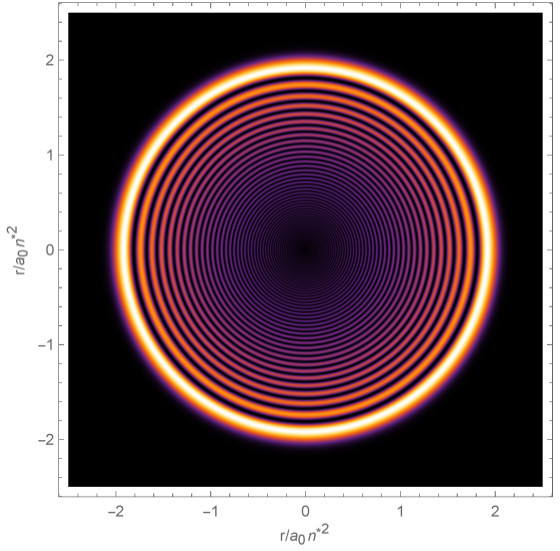
\includegraphics[width=0.6\linewidth]{figures/theory/WaveFunc_60S_}
	\caption[Fonction d'onde du niveau nS]{Probabilité de présence de l'électron dans le niveau nS : $r^2\times |R_{\mathrm{nS}}(r)|^2$, dans l'un quelconque de ses plans de symétrie.}
	\label{fig:wavefunc60S}
\end{figure}

La figure \eqref{fig:wavefunc60S} montre la probabilité de présence $r^2|R_{\mathrm{nS}}(r)|^2$ de l'électron de Rydberg dans le niveau nS du \Rb{87}.
Cela montre que la fonction d'onde se situe essentiellement loin du c\oe ur atomique et justifie donc la validité de la méthode de Numerov.

\`A partir du calcul de $R_{nl}(r)$, l'on peut aisément dériver la partie radiale de l'opérateur dipôle $\vec{d}$.
L'on apprend en particulier que la partie radiale de $\vec{d}$ entre deux niveaux de nombre quantique principal similaire varie comme $\mathcal{R} \sim a_0\cdot n^{*2}$.
Mentionnons ici que le rayon moyen de l'orbitale électronique d'un niveau de Rydberg est très similaire au calcul de la partie radiale de l'opérateur dipôle :
\begin{equation}\label{eq:orbital_size}
\braket{r_{\ket{n,l,j,m_j}}} = \int r^2dr~R_{nl}(r).r.R_{nl}(r) = \mathcal{R}(nl,nl) \propto a_0 \cdot n^{*2}.
\end{equation}
%\`A titre d'exemple, le niveau $60$S a ainsi un rayon moyen de $\braket{r} = 4850~a_0 = \numv{256.5}~\si{\nano\meter}$.
\`A titre d'exemple, l'équation \eqref{eq:orbital_size} permet d'obtenir la taille de l'orbitale électronique dans le niveau $\mathrm{60S_{1/2}}$ : son rayon moyen vaut $\braket{r} = 4850~a_0 = \numv{256.5}\si{\nano\meter}$.

	\subsection{L'effet Stark}\label{sec:Stark}
\noindent Les atomes de Rydberg étant très sensibles au champ électrique, il est important de comprendre comment celui-ci agit.
%Afin de comprendre ce phénomène plus en détail, attardons-nous à décrire l'effet Stark.
La présence d'un champ électrique constant $\vec{F}$ dans l'environnement ajoute au hamiltonien atomique un terme de couplage \og Stark \fg{}  entre le champ et l'opérateur dipolaire électrique.
En présence d'un champ électrique, le hamiltonien devient
\begin{equation}
\label{eq:hamilt_Stark}
\hat{H} = \hat{H}_0 - \vec{\hat{d} \cdot F} = \hat{H}_0 + q~\vec{\hat{r}\cdot F},
\end{equation}
où $\hat{H}_0$ est le hamiltonien libre de l'atome, dont les énergies propres sont calculées par la théorie du défaut quantique selon l'équation \eqref{eq:E_I_delta}, $\hat{\vec{r}}$ l'opérateur position de l'électron dans le potentiel atomique et $q$ la charge élémentaire, supposée positive.

Le hamiltonien Stark \eqref{eq:hamilt_Stark} perd la symétrie sphérique de $\hat{H}_0$, au profit d'une symétrie cylindrique autour de l'axe défini par le vecteur de champ électrique $\vec{F}$.
Cet axe, que nous choisirons comme étant l'axe $(Oz)$, devient alors l'axe de quantification naturel du problème.
Dans la base construite autour de cet axe, le terme d'énergie Stark prend la forme
\begin{equation}
\label{eq:dipole_Stark}
\hat{H}_S = q\hat{z}|\vec{F}| = q\hat{r} \sqrt{\frac{4\pi}{3}} Y_1^0  |\vec{F}|.
\end{equation}
où $\hat{z}$ est la composante selon $z$ de l'opérateur position, $\hat{r}$ sa norme, et $Y_
1^0$ l'harmonique sphérique $(l=1,m_l=0)$.
Ce hamiltonien ne couple que les états de même $m_l$ et vérifiant $\Delta l = \pm 1$.

Le calcul de l'effet Stark par diagonalisation du hamiltonien pour un niveau de Rydberg donné est alors simple à mener numériquement, en réduisant le sous-espace à considérer grâce à la règle de sélection $\Delta m_l = 0$.
Cette même règle de sélection permet d'imposer la condition $\Delta m_j= \Delta m_l + \Delta m_s = 0$, car l'effet Stark n'introduit aucun terme permettant de coupler des états de spins électroniques différents.
La figure \eqref{fig:Stark_60S} montre les énergies propres trouvées par diagonalisation du hamiltonien \eqref{eq:hamilt_Stark}, pour les états d'énergie proche de celle du niveau $\mathrm{60S_{1/2},m_j=1/2}$ et de même $m_j$.
%
\begin{figure}[!h]
\centering
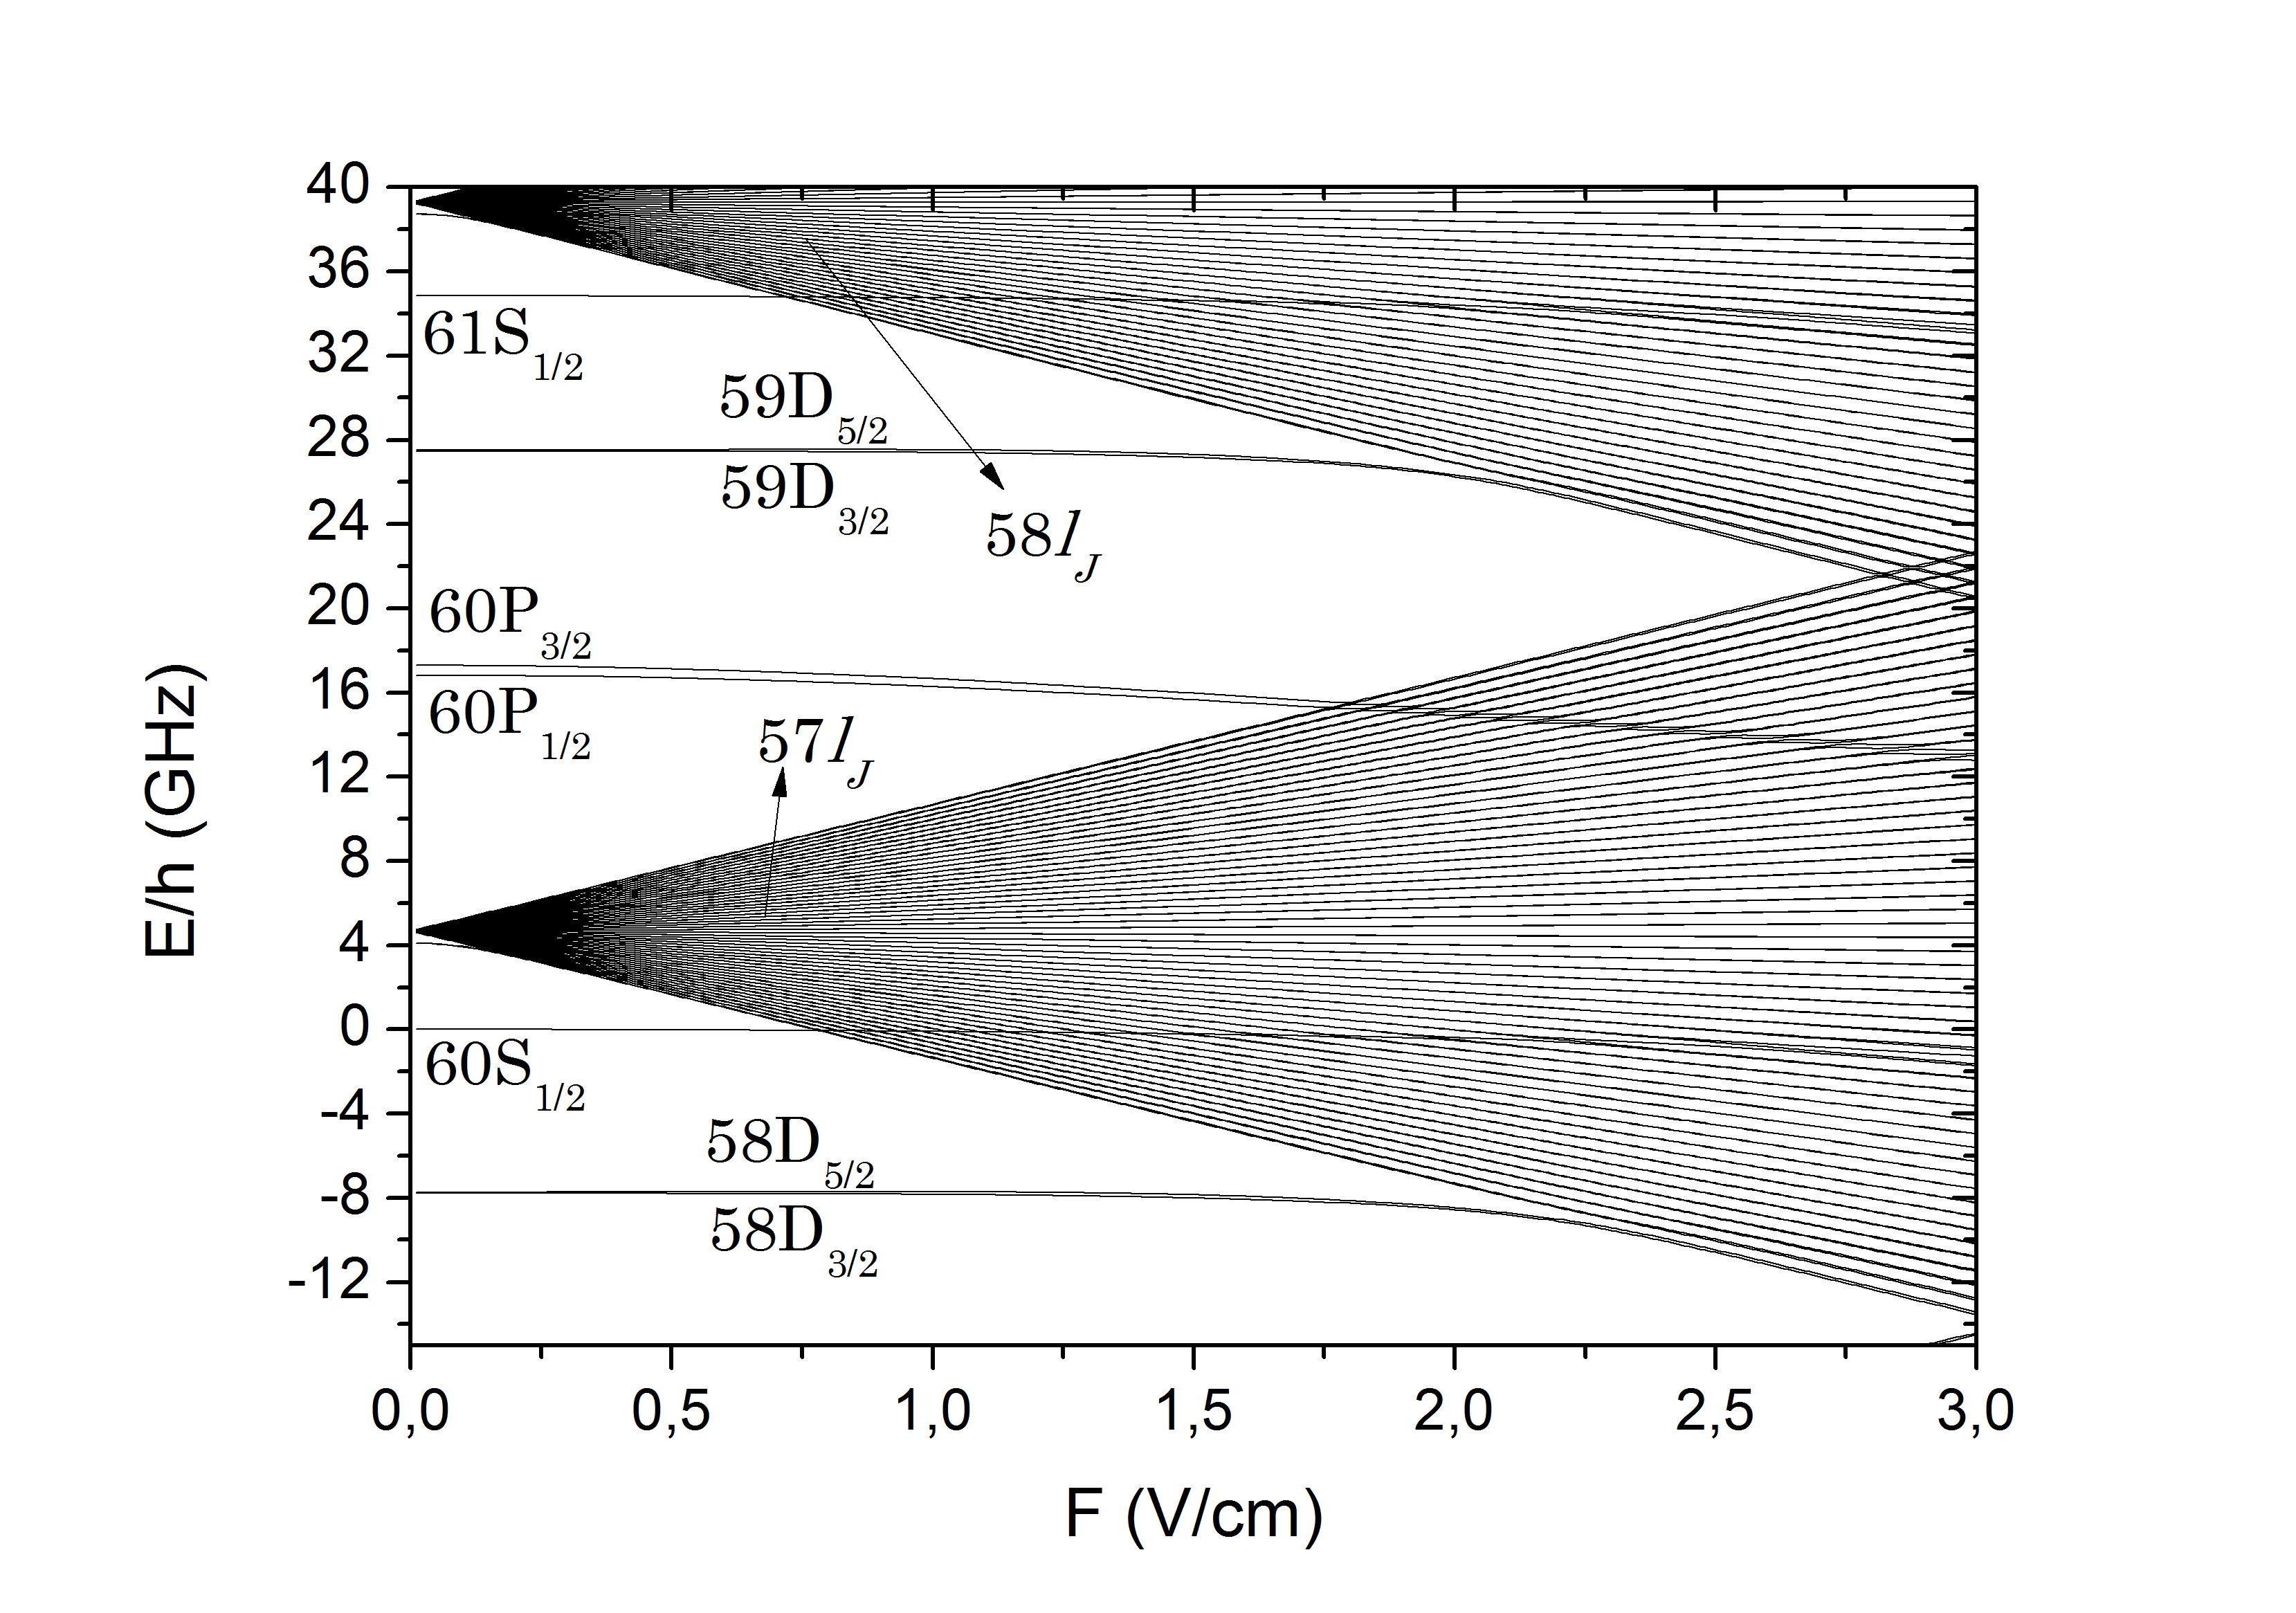
\includegraphics[width=\linewidth]{figures/setup/rydberg/Stark_60S}
\caption[Diagramme Stark autour du niveau $\mathrm{60S}$]{
Diagramme Stark autour du niveau $\mathrm{60S}$, pour les états de $m_j=1/2$.
Le défaut quantique déplace beaucoup les niveaux S,P et D.
Ces niveaux non-dégénérés ont un effet Stark quadratique en champ électrique.
Les niveaux de grand $l$ sont dégénérés et ont un effet Stark linéaire (ce sont les multiplicités qui s'ouvrent en éventail).
}
\label{fig:Stark_60S}
\end{figure}
%
Deux cas sont à distinguer. Les niveaux de faible moment orbital $l\leq 3$ sont déplacés en énergie par leur défaut quantique important.
Le terme d'interaction Stark ne couplant que des niveaux ayant la même énergie en l'absence de champ électrique, ces niveaux S,P et D ne sont perturbés qu'au second ordre par l'effet Stark.
Leur énergie varie donc de façon quadratique avec le champ électrique.
Les niveaux de grand nombre quantique orbital $l$ et de même nombre quantique principal $n$ sont, eux, dégénérés.
Le champ électrique sépare donc leurs énergies linéairement
\footnote{
Le cas de l'effet Stark pour les atomes de grand $l$ sera traité plus en détail dans le chapitre \ref{chapter:circsim}.
}.
La figure \eqref{fig:Stark_60S} montre deux telles multiplicités, $n=57$ et $n=58$.

Les niveaux de bas $l$ présentent donc tous un effet Stark quadratique que l'on exprime sous la forme
\begin{equation}
\label{eq:Stark_quad}
\Delta \nu_S = A\cdot\vec{F}^2.
\end{equation}
%On comprend mieux ainsi la forme des raies présentées en figure \eqref{fig:vieilles_raies} :
%l'effet Stark ne peut que réduire la fréquence de transition $5S-60S$ et la raie n'est donc élargie que du côté des basses fréquences.
%
La diagonalisation du hamiltonien \eqref{eq:hamilt_Stark} et l'ajustement des énergies propres ainsi calculées nous permettent d'extraire les coefficients d'effet Stark pour n'importe quel niveau.
La table \eqref{tab:Stark_60S} répertorie les coefficients d'effet Stark quadratique pour quelques niveaux autour du $\mathrm{60S}$.

\begin{table}[!h]
	\centering
	\caption[Effet Stark quadratique des niveaux proches du $\mathrm{60S}$]{Coefficients d'effet Stark quadratique des niveaux proches du $\mathrm{60S}$.
	}
	\label{tab:Stark_60S}
	\begin{tabular}{c c }
		\toprule\midrule
		Niveau de Rydberg
		& Coefficient Stark quadratique
		\\
		$\ket{n,l,j}$
		& $A_{n,l,j,m_j}$ en $\si{\MHz \per (\V \per\cm) \squared}$ \\
		\midrule
		$\mathrm{60S_{1/2}}$
		& \SI{-89.9}{} \\
		$\mathrm{61S_{1/2}}$
		& \SI{-100.9}{} \\
		$\mathrm{60P_{3/2},m_j=\pm -1/2}$
		& \SI{-676}{} \\
		$\mathrm{60P_{3/2},m_j=\pm -3/2}$
		& \SI{-569}{} \\
		\midrule
		\bottomrule
 	\end{tabular}
\end{table}

%\noindent Si l'on suppose que la largeur des spectres de la figure \eqref{fig:vieilles_raies} est due principalement à l'effet Stark causé par des gradients de champ électrique, alors ceux-ci peuvent s'estimer grâce aux coefficients données en table \eqref{tab:Stark_60S}.
%Une largeur de raie de $\SI{40}{\MHz}$ correspond à un champ électrique variant de $\SIrange{0}{0.667}{\V/\cm}$ sur l'extension du nuage.
%Or le nuage utilisé pour ces spectres était un MOT de $\sim \SI{200}{\um}$ de diamètre, ce qui nous donne une valeur de gradient de champ électrique de l'ordre de $\SI{35}{(\V/\cm)\per\cm}$.

	\subsection{Temps de vie des niveaux de Rydberg}
\noindent Avec la connaissance des dipôles de transition d'un niveau de Rydberg vers les niveaux voisins, 	il est possible de connaître le temps de vie de celui-ci.
Deux processus entrent en jeu dans la désexcitation radiative à température finie de ces niveaux atomiques :
les transitions par émission spontanée mais aussi les transitions par absorption ou émission stimulée par le rayonnement de corps noir de leur environnement.
En effet, les transitions entre niveaux de Rydberg proches en énergie sont dans le domaine des micro-ondes millimétriques.
Cela implique qu'elles seront à considérer dès les très basses températures : contrairement aux photons optiques, des photons micro-ondes sont déjà émis par le rayonnement du corps noir aux températures cryogéniques, de quelques \si{\milli\kelvin} à quelques \si{\kelvin}.

\`A titre d'exemple, la fréquence de la transition entre le niveau $\ket{60\mathrm{S}1/2}$ et le niveau $\ket{59\mathrm{P}3/2}$ vaut $\nu = E/h = \numv{18.5213}\si{\giga\hertz}$. La température de corps noir correspondant à cette fréquence est de $T=h\nu /\kb = \numv{0.89}\si{\kelvin}$.
Cette transition sera donc limitante pour le temps de vie du niveau 60S dès lors que celui-ci sera dans un environnement dépassant les $\numv{500}\si{\milli\kelvin}$.

%Or les températures de rayonnement du corps noir associées à ces gammes de fréquence se situent dans la gamme de quelques \si{\milli\kelvin} à quelques \si{\kelvin}.
\`A température nulle, le temps de vie d'un niveau excité est calculé uniquement à partir des coefficients d'Einstein pour l'émission spontanée \cite{MX_GALLAGHERBBODY}. Un électron dans un niveau excité est couplé aux niveaux de plus basse énergie par les modes électromagnétiques du vide et le taux de désexcitation d'un niveau initial $\ket{i}$ vers un niveau final $\ket{f}$ séparés d'une énergie $E_f - E_i = -\hbar \omega_{if} < 0$ est donné par :
\begin{equation}\label{eq:EinsteinAif}
A_{if} = \frac{2\omega_{if}^3}{3\epsilon_0c^3h}\cdot q^2\cdot |\bra{i}r\ket{f}|^2
\end{equation}
Ce coefficient est le produit de la densité de modes du rayonnement électromagnétique autour de la fréquence résonante $\nu_{if}=\omega_{if}/2\pi$ et du moment dipolaire de transition entre les niveaux $\ket{i}$ et $\ket{f}$ couplés par ce rayonnement.
Le temps de vie de l'état excité est alors calculé en sommant les taux d'émission spontanée vers chacun des niveaux auxquels il a accès par transition dipolaire électrique.
Les transitions dipolaires par émission d'un photon respectant la règle de sélection $\Delta l = \pm1$ et $\Delta m \leq 1$, la quantité de termes à considérer s'en trouve heureusement limitée.

\`A température finie cependant, l'absorption et l'émission stimulée vers les niveaux voisins entrent en jeu.
Le coefficient d'Einstein pour l'absorption et  l'émission stimulée s'écrit ici
\begin{equation}\label{eq:EinsteinBif}
B_{if} = A_{if} . \bar{n}(\omega_{if})
\end{equation}
Il s'agit alors de connaître, pour une température donnée, le taux d'occupation du rayonnement électromagnétique aux fréquences des transitions entre niveaux de Rydberg.
Ce taux nous est donné par la distribution de Bose-Einstein pour un gaz de bosons \cite{TXT_GORECKIPHYSTAT} :
\begin{equation}\label{eq:BoseStat}
\bar{n}(\omega) = \frac{1}{e^{\frac{\hbar\omega}{\kb T}}-1}
\end{equation}
qui devient, lorsque $\kb T \gg \hbar\omega$,
\begin{equation}\label{eq:BoseStat_blackbody}
\bar{n}(\omega) \sim \frac{\kb T}{\hbar\omega}.
\end{equation}
Le nombre de photons par mode varie alors linéairement avec la température et ces photons stimulent des transitions vers des niveaux de Rydberg proches, diminuant ainsi le temps de vie du niveau de départ.


	%\subsection{Le niveau de Rydberg 60S : $\mathbf{\ket{n=60,l=0}}$}
%\noindent Afin d'illustrer les propriétés singulières des niveaux de Rydberg, prenons un exemple qui nous sera utile par la suite : le niveau de Rydberg 60S, qui a donc un moment cinétique orbital $l=0$. Nous nous intéresserons à sa taille, à ses dipôles de transition avec les niveaux voisins, et à son temps de vie.

%Grâce à l'équation \eqref{eq:orbital_size}, nous pouvons obtenir la taille de l'orbitale électronique dans le niveau 60S : son rayon moyen vaut $\braket{r} = 4850~a_0 = \numv{256.5}\si{\nano\meter}$.
%, valeur qui paraît très grande en comparaison avec l'extension spatiale d'un atome dans le niveau fondamental qui est de l'ordre de quelques $a_0$.

\subsubsection*{Temps de vie du niveau $\mathbf{60S_{1/2}}$}
De par la règle de sélection $\Delta l=\pm1$, les termes à considérer pour les transitions dipolaires depuis le niveaux $\ket{n=60,l=0}$ sont les couplages avec les niveaux $n\mathrm{P}_j = \ket{n,l=1,j},~j\in\{1/2,3/2\}$.
La figure \eqref{fig:matrixelements} montre, pour tous les $n$, la somme des coefficients d'Einstein d'émission spontanée et d'absorption et émission stimulée à différentes températures vers les niveaux $n\mathrm{P}_j$.

\begin{figure}[th!]
	\centering
	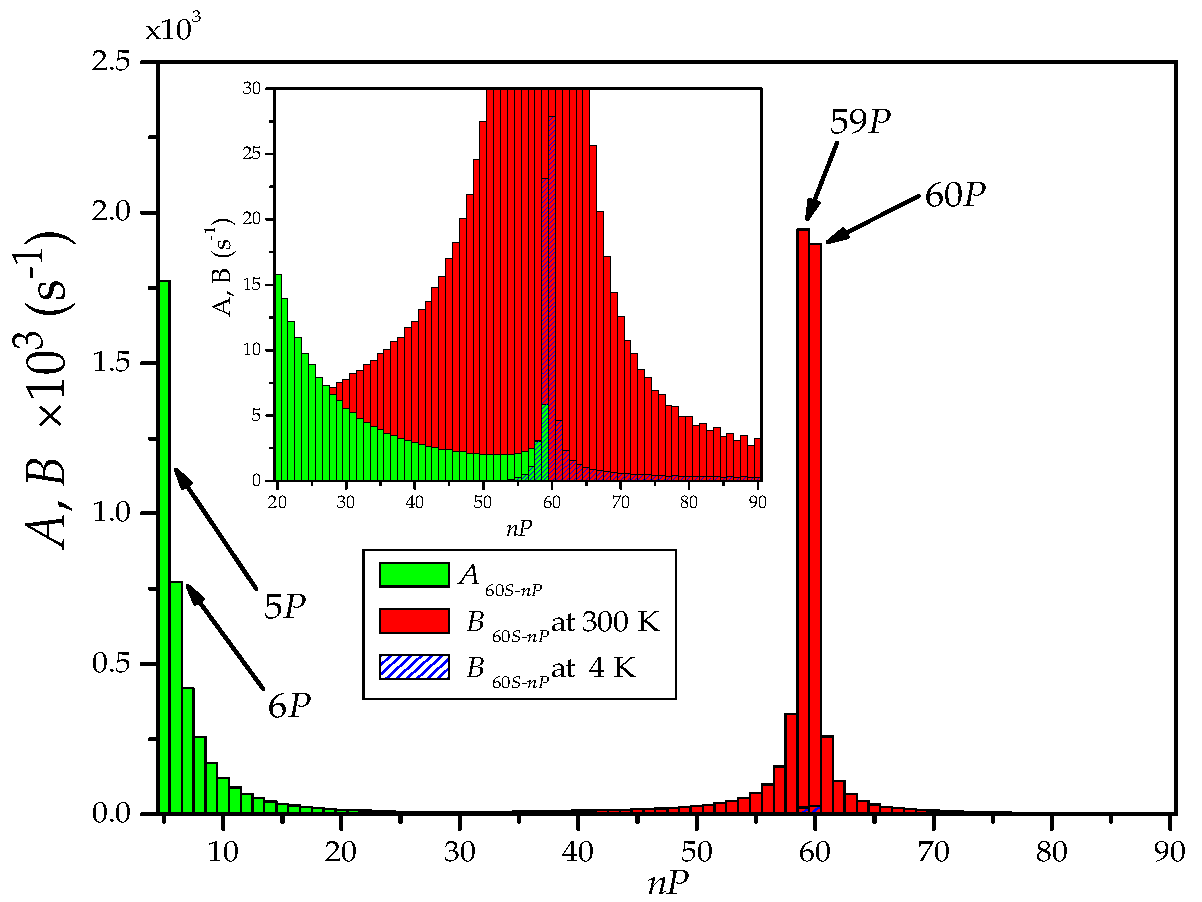
\includegraphics[width=0.7\linewidth]{figures/theory/lifetime}
	\caption[Coefficients d'Einstein de 60S vers $n\mathrm{P}_j,j\in{1/2,3/2}$]{
	Coefficients d'Einstein pour l'émission spontanée (A) et pour l'absorption et émission stimulée par le rayonnement du corps noir(B), depuis le niveau 60S vers les niveaux $n\mathrm{P}_j$.
	Pour chaque $n$, nous montrons la somme des coefficients vers $n\mathrm{P}_{j=1/2}$ et $n\mathrm{P}_{j=3/2}$.
	L'insert montre à une échelle plus adaptée la contribution du rayonnement du corps noir à $\SIv{4}{\kelvin}$.
	}
	\label{fig:matrixelements}
\end{figure}

Il est clair d'après la figure \eqref{fig:matrixelements} que le rayonnement du corps noir à $\numv{4.2}\si{\kelvin}$ contribue peu à une réduction de la durée de vie du niveau 60S par rapport à l'émission spontanée vers les niveaux de bas $n$, alors que le rayonnement du corps noir à $\numv{300}\si{\kelvin}$ aura un effet considérable, ce que confirme la table \eqref{tab:lifetime_60S}.

\begin{table}[h!]
	\centering
	\caption{Temps de vie du niveau 60S à température finie.}
	\label{tab:lifetime_60S}
	\begin{tabular}{c|c c c}
		\toprule\midrule
		\multicolumn{1}{c}{  }
		&\multicolumn{1}{c}{\text{temps de vie à }\numv{0}\si{\kelvin}}
		&\multicolumn{1}{c}{\text{temps de vie à }\numv{4.2}\si{\kelvin}}
		&\multicolumn{1}{c}{\text{temps de vie à }\numv{300}\si{\kelvin}}
		\\ 
		\midrule
		$60\mathrm{S}_{1/2}$
		&$\numv{244.5}\si{\micro\second}$
		&$\numv{239.8}\si{\micro\second}$
		&$\numv{99.4}\si{\micro\second}$\\
		\midrule
		\bottomrule
 	\end{tabular}
\end{table}

Le temps de vie du niveau 60S, de l'ordre de $\SIvv{250}{\us}$ aux températures cryogéniques, permet d'observer et manipuler celui-ci pendant des temps qui sont longs à l'échelle du mouvement d'un nuage de Rydberg.
Cependant si l'on souhaite développer une plateforme de simulation quantique, des temps d'observation beaucoup plus longs sont nécessaires.
Les atomes de Rydberg circulaires ont des durées de vie à température nulle de l'ordre de la dizaine de \si{\ms}, soit cent fois plus que le niveau 60S.
Cela fait des atomes circulaires de bons candidats pour un simulateur quantique.

\section{Les niveaux de Rydberg circulaires}\label{sec:circ_parabol}
\noindent Les niveaux de Rydberg de grand moment orbital, et en particulier les états de Rydberg circulaires, présentent une structure fine et un défaut quantique qui sont très largement négligeables.
Ils sont en cela parfaitement similaires à l'atome d'hydrogène.
On peut utiliser pour les étudier les fonctions d'onde analytiques hydrogénoïdes sans perte de précision.
Pour la même raison, le nombre quantique $j$ qui rend compte du couplage fin n'est plus nécessaire.

Les autres perturbations que peut subir le modèle de l'atome d'hydrogène, comme la présence d'un champ électrique ou magnétique extérieur en deviennent d'autant plus importantes à prendre en compte.
De plus, les niveaux circulaires étant extrêmement anisotropes, l'absence d'axe de quantification leur est préjudiciable.
Ils se mélangent alors rapidement aux niveaux voisins et il est utile de leur imposer un champ électrique, même faible, afin de pallier ce problème.
%En premier lieu, le champ extérieur définit un axe de quantification pour le moment cinétique orbital de l'atome.
%Au cours de ce paragraphe, nous considérerons qu'un axe de quantification est défini selon $(Oz)$ par un champ électrique.
%%, mais nous négligerons pour le moment l'effet Stark, par lequel la présence d'un champ électrique extérieur influence les niveaux électroniques.
%La présence d'un champ selon l'axe privilégié $(Oz)$ brise la symétrie sphérique du problème et la description des fonctions d'onde en coordonnées sphériques, donc sur la base des harmoniques sphériques, n'est plus la mieux adaptée à la situation.

\subsection{La base des états paraboliques}
\noindent	La construction de la base des harmoniques sphériques était fondée sur la conservation du moment cinétique lors du mouvement et sur l'ensemble complet d'opérateurs qui commutent (\og ECOC \fg{}) $\{\hat{H} , \hat{L}^2 , \hat{L}_z \}$
\footnote{
On a ici oublié la structure fine, qui exige lorsqu'elle est prise en compte, de remplacer $\hat{\vec{L}}$ par $\hat{\vec{J}}= \hat{\vec{L}}+\hat{\vec{S}}$.
}.%, où $\hat{J}=\hat{L}+\hat{S}$ est le moment cinétique total de l'électron.
En présence d'un champ électrique extérieur définissant l'axe $(Oz)$, le terme de couplage Stark $-\hat{\vec{d}}\cdot\vec{F} = q\hat{z}|\vec{F}|$ (cf équation \ref{eq:hamilt_Stark}) brise la symétrie sphérique du problème, de façon telle que l'opérateur $\hat{L}^2$ ne commute plus avec le hamiltonien du système.
%Rien ne contrarie cet invariant ici, mais il peut être utile d'en dégager un deuxième.
Il est alors nécessaire de trouver un nouvel invariant du mouvement, qui permettra de définir un nouvel ECOC.
Celui-ci pourra toujours contenir $\hat{L_z}$, qui reste un bon opérateur.

Dès lors que la fonction d'onde électronique reste loin du c\oe ur atomique, l'interaction entre l'électron de valence et le c\oe ur se réduit à un mouvement à force centrale.
La mécanique céleste a traité extensivement des mouvements à force centrale, et nous apprend qu'ils ont en commun l'invariance du vecteur de Runge-Lenz, qui caractérise l'excentricité des trajectoires des corps.
%
L'analogie entre l'interaction gravitationnelle des corps célestes et l'interaction coulombienne au sein des atomes permet de définir l'opérateur vectoriel :
\begin{equation}\label{eq:RungeLenz}
\hat{\vec{A}} = \frac{1}{\sqrt{-2m_e E}} \left( \frac{1}{2} (\hat{\vec{p}}\wedge\hat{\vec{L}} - \hat{\vec{L}}\wedge\hat{\vec{p}}) - m_e e^2 \frac{\vec{r}}{r} \right).
\end{equation}
Cet invariant commute avec le hamiltonien de l'atome d'hydrogène et est de même dimension que l'opérateur de moment orbital $\vec{\hat{L}}$.
Les vecteurs propres de $\hat{\vec{A}}$ prennent donc une forme similaire à ceux de $\hat{\vec{L}}$ et ses valeurs propres varient de $0$ à $\hbar(n-1)$.
%Les relations de commutation des opérateurs $\hat{L}_i$ et $\hat{a}_j$ permettent de construire un opérateur vectoriel $\{\hat{a}_x,\hat{a}_y,\hat{L}_z\}$ vérifiant les relations de commutation d'un moment cinétique :
%\begin{equation} \label{eq:commut_Leta}
%\left\{
%\begin{aligned}
%&[\hat{a}_x,\hat{a}_y]=i\hat{L}_z \\
%&[\hat{a}_y,\hat{L}_z]=i\hat{a}_x \\
%&[\hat{L}_z,\hat{a}_x]=i\hat{a}_y .\\
%\end{aligned}
%\right.
%\end{equation}
%Ce vecteur est donc un générateur des rotations dans l'espace à trois dimensions, défini par les coordonnées $\{ \text{excentricité selon }(Ox), \text{ excentricité selon }(Oy), \text{moment cinétique selon }(Oz)\}$.

Malheureusement, les opérateurs $\hat{\vec{L}}$ et $\hat{\vec{A}}$ ne commutent pas.
Il est donc nécessaire, afin d'obtenir une bonne base de description, de construire de nouveaux opérateurs qui commutent entre eux et vérifient les relations de commutation d'un moment cinétique à trois dimensions.
Les opérateurs
\begin{equation}\label{eq:defJ1J2}
\begin{aligned}
&\hat{\vec{J}}_1 = \frac{1}{2}\left( \hat{L} - \hat{A} \right)\\
\text{et} & \\
&\hat{\vec{J}}_2 = \frac{1}{2}\left( \hat{L} + \hat{A} \right).
\end{aligned}
\end{equation}
vérifient ces propriétés, et commutent avec le hamiltonien.
Au sein d'une même multiplicité, ces opérateurs vérifient 
\begin{equation}\label{eq:defJ1J2sq}
\hat{\vec{J}}_1^2 = \hat{\vec{J}}_2^2 = -\frac{\hbar^2}{4}-\frac{m_ee^4}{8E_n},
\end{equation}
ce qui s'écrit aussi
\begin{equation}\label{eq:E_j1_j2}
E=-\frac{m_ee^4}{2\hbar^2(2j_1+1)^2}=-\frac{m_ee^4}{2\hbar^2(2j_2+1)^2}~.
\end{equation}
L'on retrouve ici le fait que pour une énergie $E$ fixée et donc au sein d'une multiplicité de nombre quantique principal $n$, $\hat{\vec{J}}_1$ et $\hat{\vec{J}}_2$ définissent chacun un moment cinétique $j_{1,2}=(n-1)/2$.

Les états propres au sein d'une même multiplicité sont alors obtenus en diagonalisant $\hat{\vec{J}}_1^2$, $\hat{\vec{J}}_2^2$ et les composantes $\hat{J}_{1z}$ et $\hat{J}_{2z}$.
En notant $\hbar m_{1,2}$ les valeurs propres de $\hat{J}_{1,2~z}$, on pourra caractériser les états propres par les nombres $\{j_1,m_1,j_2,m_2\}$.
Or pour $n$ fixé, $j_1=j_2=(n-1)/2$. Ainsi, un état propre sera entièrement défini par les nombres quantiques $\ket{n,m_1,m_2}$, avec $m_1$ et $m_2$ variant entre $-(n-1)/2$ et $+(n-1)/2$.
Par construction de $\hat{\vec{J}}_{1,2}$, il est aisé de retrouver le nombre quantique magnétique $m=m_1+m_2$.
La figure \eqref{fig:parab_m1m2} propose une représentation schématique des niveaux $\ket{m_1,m_2}$ d'une même multiplicité $n$.

\begin{figure}[!h]
\centering
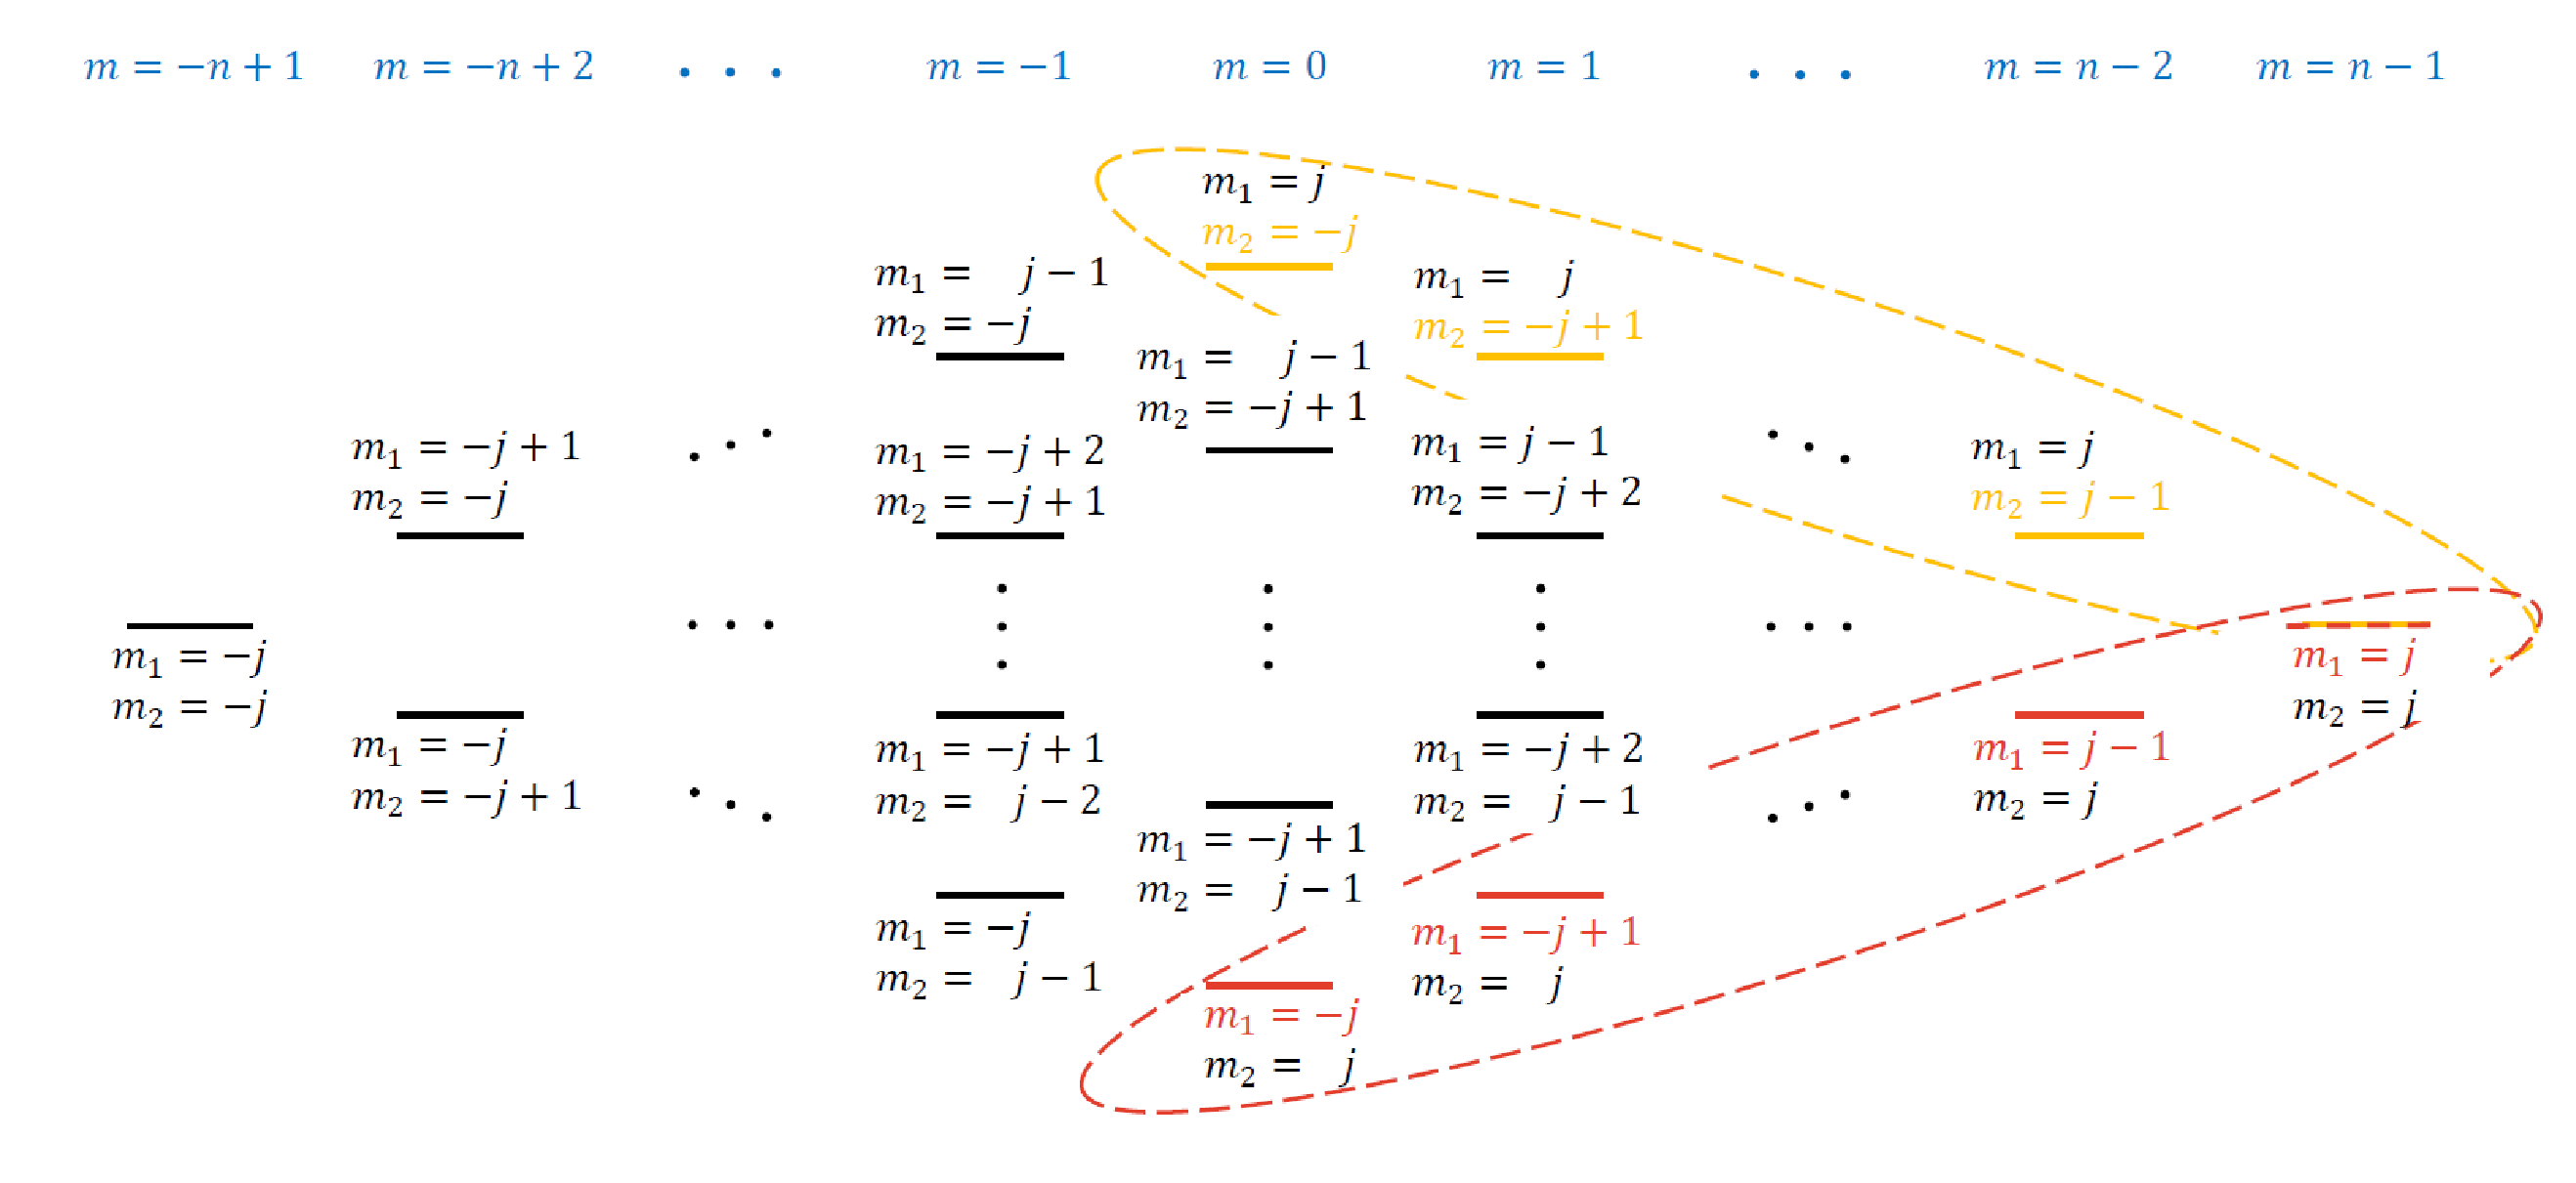
\includegraphics[width=1.\linewidth]{figures/theory/echelle_parabolique_m1m2}
\caption[Échelle des niveaux paraboliques $\ket{n,m_1,m_2}$]{
Niveaux paraboliques $\ket{n,m_1,m_2}$ de même nombre quantique principal $n$, classés horizontalement en fonction de leur nombre quantique magnétique $m=m_1+m_2$. Le nombre $j=j_1=j_2$ est la valeur des moments cinétiques $\hat{\vec{J}}_1$ et $\hat{\vec{J}}_2$ et vaut $j=(n-1)/2$.
La diagonale jaune représente la direction de variation de $m_2$ à $m_1$ fixé et la diagonale rouge la direction de variation de $m_1$ à $m_2$ fixé.
}
\label{fig:parab_m1m2}
\end{figure}


%L'équation de Schrödinger peut s'écrire dans les coordonnées paraboliques $(\xi ,\eta ,\phi )$ obtenues à partir des coordonnées sphériques $(r,\theta ,\phi)$ par la transformation :
%\begin{equation}\label{eq:coordParab}
%\hfill \xi = r(1+\cos\theta) \hfill \eta = r(1-\cos\theta)\hfill
%\end{equation}
%Dans ce système de coordonnées, l'équation de Schrödinger est séparable à condition d'introduire les nombres quantiques $n_1$ et $n2$.
%La base des états paraboliques s'obtient en introduisant les nombres quantiques paraboliques $n_1$ et $n_2$ qui sont fonction de $m_1$ et $m_2$.
%Nous préférerons ici une autre approche pour la plus grande simplicité avec laquelle elle permet de représenter les états atomiques.
%Introduisons à cet effet

Afin d'aider à la représentation des états atomiques, introduisons un nouveau nombre quantique $k=m_1-m_2$, qui quantifie l'excentricité de l'orbite électronique et permet de transformer la base $\ket{n,m_1,m_2}$ en la base $\ket{n,m,k}$ :
\begin{equation}\label{eq:base_nmk}
\left\{
\begin{aligned}
&n \text{ \begin{small}
le nombre quantique principal
\end{small}}\\
&m \text{ \begin{small}
le nombre quantique magnétique variant de
\end{small} }
-(n-1)~~ \text{ \begin{small} à \end{small}} ~~(n-1)\\
&k=m_1-m_2 \text{ \begin{small} variant de\end{small} } (|m|-(n-1))~~ \text{ \begin{small} à \end{small} } ~~(-|m|+n-1).
\end{aligned} \right.
\end{equation}
%


\begin{figure}[!h]
\centering
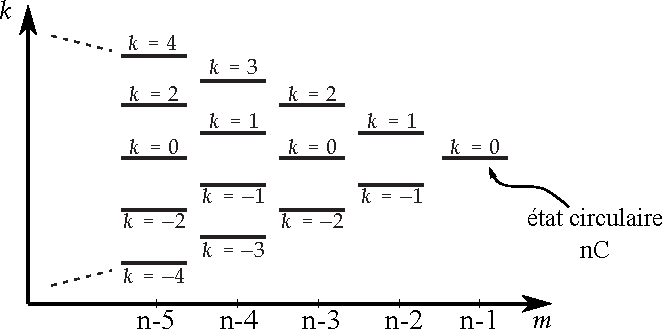
\includegraphics[width=.7\linewidth]{figures/theory/echelle_parabolique_mk}
\caption[Échelle des niveaux paraboliques $\ket{n,m,k}$]{
Niveaux paraboliques $\ket{n,m,k}$ de même nombre quantique principal $n$, classés horizontalement en fonction de leur nombre quantique magnétique $m$ et étiqueté selon le nombre quantique $k$.
Seuls les niveaux de très grand $m$ sont représentés.
}
\label{fig:parab_mk}
\end{figure}

\noindent La figure \eqref{fig:parab_mk} propose une représentation schématique des niveaux $\ket{m,k}$ de $m$ très élevé au sein d'une multiplicité $n$.

Le niveau de $m$ maximal dans une multiplicité donnée, $\ket{n,m=n-1,k=0} =\ket{n,l=n-1,m=l}$, est appelé le niveau circulaire nC.
Sa fonction d'onde électronique se réduit à un tore éloigné du c\oe ur atomique, de rayon $\sim n(n-1)a_0$, et contenu dans le plan perpendiculaire à l'axe de quantification.
La figure \eqref{fig:wavefunc50C} montre la probabilité de présence $r^2|R(r)|^2$ de l'électron dans le plan perpendiculaire à l'axe de quantification, pour le niveau de Rydberg nC. Celle-ci a une présente un rayon moyen valant
\begin{equation}\label{eq:rayon_nC}
\braket{r_{\ket{\mathrm{nC}}}}\simeq  a_0 \cdot n^2.
\end{equation}
Les niveaux de $m$ élevé mais non maximal seront appelés niveaux elliptiques en raison de la forme de leurs fonctions d'onde et seront étiquetés sur la base $\ket{n,m,k}$.
\begin{figure}[!h]
	\centering
	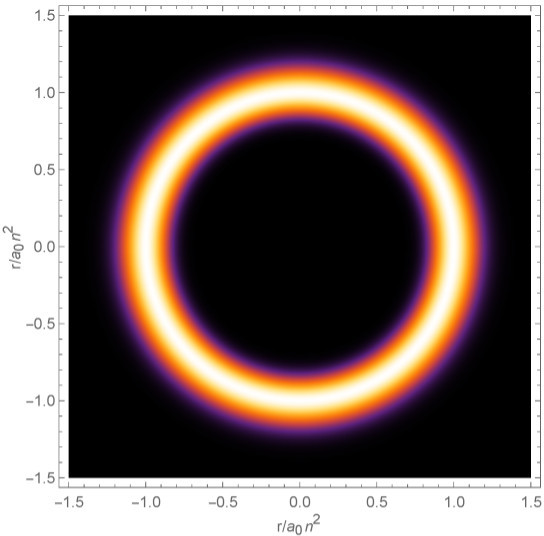
\includegraphics[width=0.5\linewidth]{figures/theory/WaveFunc_50C_}
	\caption[Fonction d'onde du niveau nC]{Probabilité de présence de l'électron dans le niveau nC : $r^2\times |R_{n\mathrm{C}}(r)|^2$, dans le plan perpendiculaire à l'axe de quantification et passant par le noyau.
	Celle-ci décrit un tore de rayon $n^2a_0$ autour du c\oe ur atomique.}
	\label{fig:wavefunc50C}
\end{figure}

%Les circulaires ont besoin d'un champ électrique pour se stabiliser.
\subsubsection*{L'effet Stark pour les atomes de grand moment cinétique}
\noindent Comme nous l'avons dit en \ref{sec:Stark}, dans la base parabolique construite autour de l'axe $(Oz)$ défini par la direction du champ électrique, le terme de couplage Stark prend une forme simple donnée par l'équation \eqref{eq:dipole_Stark} :
\begin{equation}
\label{eq:dipole_Stark2}
\hat{H}_S = q\hat{z}|\vec{F}| = q\hat{r} \sqrt{\frac{4\pi}{3}} Y_1^0  |\vec{F}|.
\end{equation}
%
Dans le cas des niveaux de Rydberg à grand moment cinétique, l'absence de défaut quantique permet de résoudre ce hamiltonien analytiquement par un traitement perturbatif de la forme \cite{TXT_BETHE_ONELECTRONATOMS} 
\begin{equation}
\label{eq:perturbative_energy}
E = E^{(0)}+E^{(1)}+E^{(2)}+\dots,
\end{equation}
où les termes du développement s'écrivent
\begin{equation}
\label{eq:Stark_circular}
\begin{aligned}
&E^{(0)}/2E_I = -\frac{1}{2n^2} \\
&E^{(1)}/2E_I = \frac{3}{2}nk|\vec{F}|*\frac{ea_0}{2E_I} \\
&E^{(2)}/2E_I = -\frac{1}{16}\cdot (19+17n^2-9m^2-3k^2) \cdot n^4|\vec{F}|^2*\left( \frac{ea_0}{2E_I}\right) ^2,
\end{aligned}
\end{equation}
%
en unités du système international.
On remarque ici que les états à $k=0$, et en particulier l'état circulaire, ne subissent l'effet Stark qu'au second ordre.

Nous pouvons désormais représenter les niveaux paraboliques $\ket{n,m,k}$ en présence d'un champ électrique qui lève leur dégénérescence.
La figure \ref{fig:parab_mk} se transforme alors en la figure \ref{fig:Stark_nmk}.
%
\begin{figure}[!h]
\centering
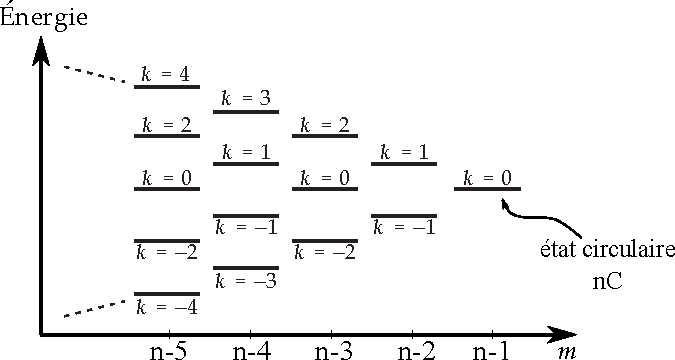
\includegraphics[width=.8\linewidth]{figures/theory/Stark_nmk}
\caption[Échelle des niveaux paraboliques $\ket{n,m,k}$]{
Énergie des niveaux paraboliques $\ket{n,m,k}$ de même nombre quantique principal $n$ en présence d'un champ électrique.
Les niveaux sont classés horizontalement en fonction de leur nombre quantique magnétique $m$ et étiqueté selon le nombre quantique $k$.
Seuls les niveaux de très grand $m$ sont représentés.
}
\label{fig:Stark_nmk}
\end{figure}
%
%Ce diagramme Stark ne ressemble pas à celui des multiplicités $n=57$ et $n=58$ de la figure \eqref{fig:Stark_60S}.
%En effet, ces multiplicités étaient définies non seulement pas leur nombre quantique principal $n$, mais aussi par leur nombre quantique magnétique $m_j = 1/2$.
%Ici au contraire, seul $n$ est fixé.

\subsection{Le niveau de Rydberg 50C : $\ket{n=50,l=49,m_l=49}$}\label{subsec:level_50C}

\noindent Parmi les niveaux de Rydberg circulaires, le niveau 50C sera d'un intérêt particulier pour nous.
Ce niveau circulaire $n=50$ a une taille valant $\braket{r}_{50C} \simeq 50^2 a_0 = 2500 a_0 = \numv{132}\si{\nano\meter}$.
	

En ce qui concerne leur temps de vie, les niveaux de Rydberg circulaires ont une différence essentielle avec les niveaux de faible $l$ : les niveaux circulaires n'ont de transition dipolaire possible que vers des niveaux eux aussi à très grand $l$, et donc à très grand $n$.
Il n'y a d'ailleurs qu'une seule transition spontanée possible depuis le niveau circulaire $\text{nC}=\ket{n,l=n-1,m_l=l}$, c'est celle vers le niveau circulaire $\text{(n-1)C}=\ket{n'=n-1,l'=n'-1,m_l'=l'}$.
En effet, il n'existe aucun niveau de plus basse énergie que $\mathrm{nC}$ mais qui aurait un $l$ qui lui soit égal ou supérieur.
La figure \eqref{fig:spontem_50C49C} représente les schémas de niveaux près de l'état circulaire $n=50$ et met en évidence l'absence de toute autre transition par émission spontanée depuis le niveau 50C.
Le niveau 50C ne peut donc se désexciter spontanément que vers le niveau 49C, ce qui réduit considérablement la contribution de l'émission spontanée à son taux de désexcitation radiative.
Le calcul du dipôle de transition $\braket{50\text{C}|\hat{\vec{d}}|49\text{C}}$ donne une valeur de $\numv{1704.71} e a_0$.
En appliquant l'équation \eqref{eq:EinsteinAif} à la fréquence de transition $\mathrm{50C}\rightarrow \mathrm{49C}$ de $\SIv{54.25955}{\giga\hertz}$, on obtient un taux de désexcitation valant $\Gamma_{50C}(\SIvv{0}{\kelvin}) = A_{i=50C-f=49C} = \SIv{34.9056}{\hertz}$.
Le temps de vie à température nulle du niveau 50C est donc de $\tau_{0,50C} = \SIv{28.65}{\ms}$, soit cent fois plus que pour le niveau 60S.
\begin{figure}[!h]
	\centering
	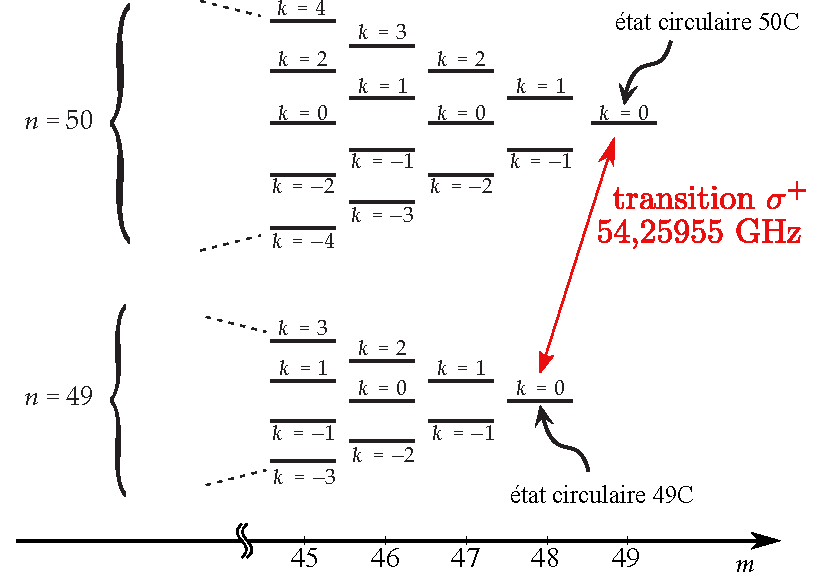
\includegraphics[width=.8\linewidth]{figures/theory/spontem_50C49C}
	\caption[Schéma de niveaux 50C-49C]{Schéma de niveaux des multiplicités $n=50$ et $n=49$ près des niveaux 50C et 49C, en présence d'un champ électrique. La seule transition possible par émission spontanée depuis le 50C est la transition vers le 49C.}
	\label{fig:spontem_50C49C}
\end{figure}

%La limitation de la durée de vie du niveau 50C provient donc en premier lieu de l'absorption et de l'émission stimulée par le rayonnement du corps noir vers les niveaux accessibles par transition dipolaire électrique.
Étant donné le faible taux de désexcitation spontanée du niveau 50C, l'effet du rayonnement du corps noir sur sa durée de vie sera important dès les très basses températures.
Le rayonnement du corps noir amplifiera non seulement le taux de désexcitation vers le niveau 49C, mais autorisera également par absorption les transitions vers les niveaux de $n$ supérieur.
Ainsi, alors que la réduction du temps de vie du niveau 60S entre $\numv{0}\si{\kelvin}$ et $\numv{4.2}\si{\kelvin}$ est faible (voir table \ref{tab:lifetime_60S}, la durée de vie du 60S est réduite de $(1-\numvv{239.8}/\numvv{244.5}) = 2\%$), la réduction du temps de vie du niveau 50C entre $\SIvv{0}{\K}$ et $\SIvv{4.2}{\K}$ est bien plus importante et se porte à $(1-\numv{8.36}/\numv{28.65}) = 71\%$.
\`A température ambiante de $\numv{300}\si{\kelvin}$, la durée de vie de 50C est même réduite à $\numv{122}\si{\micro\second}$, très similaire à celle du niveau 60S.
La figure \eqref{fig:lifetime_50C} montre l'évolution de la durée de vie du niveau 50C en fonction de la température de rayonnement du corps noir, calculée à partir des équations \eqref{eq:EinsteinBif} et \eqref{eq:BoseStat}.


\begin{figure}[!h]
	\centering
	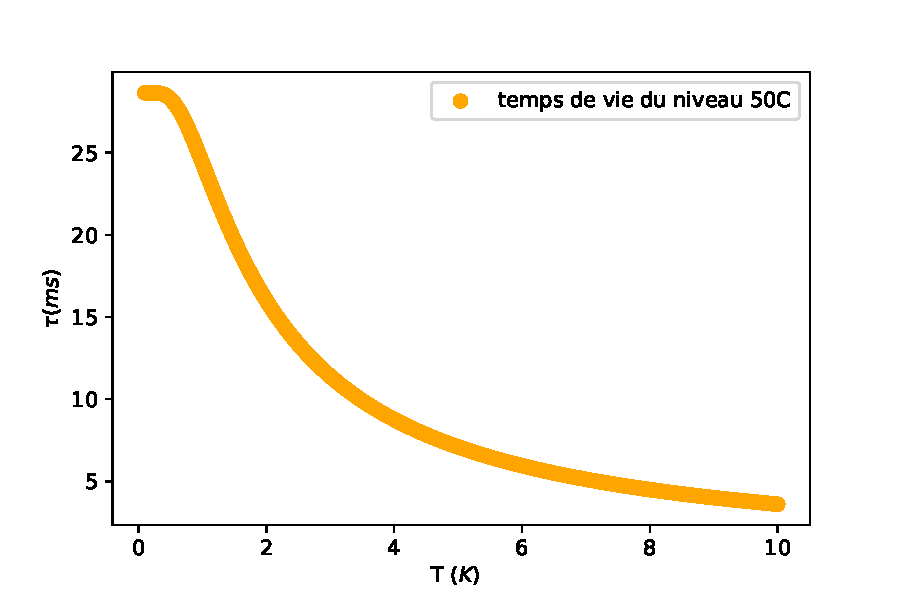
\includegraphics[width=0.8\linewidth]{figures/theory/lifetime_50C}
	\caption[Durée de vie du niveau 50C]{Durée de vie radiative du niveau de Rydberg 50C en fonction de la température de rayonnement du corps noir.}
	\label{fig:lifetime_50C}
\end{figure}

\newpage
Nous avons désormais une bonne connaissance des caractéristiques des atomes de Rydberg individuels, en particulier dans les niveaux 60S et 50C.
Ce sont de très grands atomes, avec de très grands moments dipolaires de transition, et un temps de vie très long.
Comment se comportent ces atomes de Rydberg lorsqu'ils ne sont plus isolés mais proches les uns des autres ?

%\section{Atomes de Rydberg en interaction}
%	\subsection{Deux atomes de Rydberg}
%		\noindent hamiltonien d'interaction entre deux dipôles
%		\[
%		V_{dd} = \frac{1}{4\pi\epsilon_0 r^3} \left( \mathbf{d_1}\cdot \mathbf{d_2} - 3(\mathbf{d_1}\cdot \frac{\mathbf{r}}{r})(\mathbf{d_2}\cdot\frac{\mathbf{r}}{r}) \right)
%		\]
%		\noindent de l'interaction dipole-dipole générale au terme de van der Waals en $1/r^6$ \\
%		\noindent terme d'énergie et terme d'échange
%	\subsection{les interactions entre Rydberg de bas $l$}
%		\noindent origine du $C_6$ pour 60s-60s et $C_6/A_6$ avec les voisins\\
%		reprendre Raul.figI.3 qui présente la partie radiale du dipôle 60s-ns en fonction de n\\
%		\noindent principe du blocage dipolaire et facilitation (rapide)
%	\subsection{les interactions entre Rydberg circulaires}
%		\noindent $C_6$ pour 50c-50c et $C_6/A_6$ avec les voisins \\
%		\noindent attention à l'anisotropie\\
%		équivalent de la figure ci dessus (Raul.figI.3) pour les 50c, à modifier pour l'anisotropie

\section{Atomes de Rydberg en interaction}\label{sec:interacting_rydbergs}
Dans cette thèse, nous allons nous intéresser aux interactions entre plusieurs atomes de Rydberg voisins, dans des niveaux identiques ou proches en énergie.
Le reste de ce chapitre est consacré au calcul de ces interactions et à leur application aux deux cas qui nous concernent : autour des niveaux 60S et 50C.

	\subsection{Deux atomes de Rydberg qui se parlent}
L'opérateur de moment dipolaire entre deux niveaux de Rydberg proches est grand, comme nous l'avons évoqué.
En cela, les atomes de Rydberg sont de très bonnes antennes pour le rayonnement électromagnétique lorsque celui-ci est résonant avec les fréquences de transition entre niveaux proches.
Cette caractéristique s'accentue fortement lorsque le nombre quantique principal augmente, car le moment dipolaire varie en $n^{*2}$.
Ces grands moments de transition dipolaires font aussi apparaître une interaction importante entre deux atomes de Rydberg différents : bien qu'ils restent des objets neutres électriquement, ces grands dipôles se voient très bien de loin.
En électromagnétisme classique, le terme de couplage entre deux dipôles électriques s'écrit \cite{TXT_JACKSON}
\begin{equation}\label{eq:classicDipole}
V_{dd}(\vec{r}) = \frac{1}{4\pi\epsilon_0 r^3} \left( \vec{d_1}\cdot \vec{d_2} - 3(\vec{d_1}\cdot \frac{\vec{r}}{r})(\vec{d_2}\cdot\frac{\vec{r}}{r}) \right)
\end{equation}
où $\vec{d_1}$ décrit le premier dipôle, $\vec{d_2}$ le deuxième dipôle et $\vec{r}$ le vecteur d'espace qui les sépare.
On peut alors écrire, par analogie, le hamiltonien d'interaction entre deux atomes en remplaçant les dipôles classiques par les opérateurs dipôle électrique de chaque atome.
La distance entre les atomes sera cependant traitée de façon classique, en supposant que la distance entre les atomes est très grande devant l'extension spatiale de leurs fonctions d'onde.
% C'est ce qu'on appelle l'approximation dipolaire. FAUX (commentaire Michel 15 sept
Le potentiel d'interaction dipolaire s'écrit dans ce cas
\begin{equation}\label{eq:quantDipole}
\begin{aligned}
\hat{V}_{dd}(\vec{r}) &= \frac{1}{4\pi\epsilon_0 r^3} \left( \vec{\hat{d}_1}\cdot \vec{\hat{d}_2} - 3(\vec{\hat{d}_1}\cdot \frac{\vec{r}}{r})(\vec{\hat{d}_2}\cdot\frac{\vec{r}}{r}) \right) \\
&= \frac{q^2}{4\pi\epsilon_0 r^3} \left( \vec{\hat{r}_1}\cdot \vec{\hat{r}_2} - 3(\vec{\hat{r}_1}\cdot \frac{\vec{r}}{r})(\vec{\hat{r}_2}\cdot\frac{\vec{r}}{r}) \right).
\end{aligned}
\end{equation}
%
Remarquons que ce terme dépend du produit des opérateurs de transition dipolaire électrique de chaque atome. L'interaction entre atomes de Rydberg varie donc comme $(n^{*2})^2 = n^{*4}$. 

Calculer l'interaction entre deux atomes de Rydberg revient à diagonaliser le hamiltonien total du système des deux atomes dans l'espace de Hilbert des états possibles pour la paire d'atomes.
Sans autre \textit{a priori}, une base naturelle pour cet espace est le produit tensoriel $\ket{R_1}\otimes\ket{R_2}$ des états de chaque atome.
Dans cette base, le hamiltonien du système s'écrit
\begin{equation}\label{eq:hamilt2atoms}
\hat{H} = \hat{H}_{0,1} + \hat{H}_{0,2} + \hat{V}_{dd}(\vec{r})
\end{equation}
où $\hat{H}_{0,i}$ est le hamiltonien de l'atome $i$ isolé.

En l'absence de champ électrique ou magnétique extérieur, l'axe de quantification pour les niveaux de chaque atome n'est pas déterminé.
Il semble naturel de choisir alors comme axe de quantification le vecteur qui sépare les atomes.
Dans cette géométrie, le potentiel d'interaction dipolaire prend la forme
\begin{equation}\label{eq:Vdd_rr1r2}
\begin{aligned}
\hat{V}_{dd}(\vec{r})=&
-\frac{q^2}{4\pi\epsilon_0}\frac{\hat{r}_1\hat{r}_2}{r^3}\frac{4\pi}{3} \times
\left( \hat{Y}^1_1(\theta_1,\phi_1) \hat{Y}^{-1}_1(\theta_2,\phi_2) \right. \\
&\left. + \hat{Y}^{-1}_1(\theta_1,\phi_1) \hat{Y}^{1}_1(\theta_2,\phi_2)
+ 2\hat{Y}^{0}_1(\theta_1,\phi_1) \hat{Y}^{0}_1(\theta_2,\phi_2)
\right)
\end{aligned}
\end{equation}
où les $Y^{m_l}_l$ sont les harmoniques sphériques, solutions des équations de Legendre \cite{TXT_COHEN1FR}.
Dans cette base, l'opérateur $\hat{V}_{dd}$ préserve le nombre quantique magnétique total $M=m_{j1}+m_{j2}$.
Cette condition définit un sous-espace des niveaux de même $M$ pour la paire d'atomes, sous-espace qui a une dimension infinie.
Il sera donc nécessaire, pour calculer l'interaction entre les deux atomes, de tronquer ce sous-espace.
Dans le sous-espace tronqué, nous pouvons diagonaliser le hamiltonien \eqref{eq:hamilt2atoms} pour chaque distance interatomique $r$.

\subsection{Deux atomes dans le même niveau de Rydberg}\label{subsec:interaction_same_level}
Dans le cas de deux atomes dans le même niveau de Rydberg $a$, la règle de sélection $\Delta l = \pm 1$ impose que $\braket{aa|\hat{V}_{dd}|aa} = 0$.
L'opérateur d'interaction dipolaire n'agit donc sur la paire $\ket{aa}$ que comme une perturbation de second ordre, \textit{via} le couplage à des niveaux de paire intermédiaires $\ket{cd}$.
La figure \eqref{fig:Dip_aacd} représente ce couplage au second ordre.
L'énergie d'interaction résultant de cette perturbation prend la forme
\begin{equation}\label{eq:VdW_aacd}
hC_{aa}(r)=\sum_{\ket{cd}}{\frac{\braket{aa|\hat{V}_{dd}|cd}\braket{cd|\hat{V}_{dd}|aa}}{2E_a - E_c - E_d}}  = \frac{hC_{6,aa}}{r^6}
\end{equation}
où $E_i$ est l'énergie d'un atome de Rydberg individuel dans l'état $i$.
L'interaction dipolaire prend donc la forme d'une interaction de van der Waals en $1/r^6$, avec un coefficient valant $C_{6,aa}$.

\begin{figure}[!h]
\centering

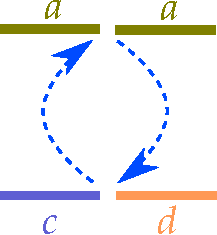
\includegraphics[width=0.3\linewidth]{figures/theory/dipole_coupling_aacd}
\caption[Couplage dipolaire entre mêmes niveaux de Rydberg]{Schéma du couplage dipolaire entre deux atomes dans des niveaux de Rydberg $a$ identiques : le couplage s'effectue au second ordre \textit{via} les niveaux $c$ et $d$.}
\label{fig:Dip_aacd}
\end{figure}

La situation se complique lorsque l'un des niveaux intermédiaires $\ket{cd}$ est quasi-dégénéré avec le niveau $\ket{aa}$, c'est-à-dire lorsque $\braket{aa|\hat{V}_{dd}|cd} \gg |2E_a-E_c-E_d|$.
Le développement perturbatif est en effet invalidé sous cette condition et il est nécessaire de traiter le problème différemment.
Si $\ket{c}=\ket{d}$, alors le sous-espace à observer est composé des deux états $\ket{aa}$ et $\ket{cc}$ et l'on a $E_c\simeq E_a$.
Le hamiltonien d'interaction s'écrit alors
\begin{equation}\label{eq:forster_aacc}
H_{aa-cc} = \bordermatrix{~ 	&\ket{aa} 	& \ket{cc} \cr
	\ket{aa}		&2E_a 		& \frac{\Braket{aa|V_{dd}|cc}}{r^3}	\cr 
	\ket{cc} 		& \frac{\Braket{aa|V_{dd}|cc}}{r^3} 		&2E_a\cr} \ .
\end{equation}
%
Les états propres de ce hamiltonien sont les combinaisons symétrique et antisymétrique $(\ket{aa}\pm\ket{cd})/\sqrt{2}$, et présentent les énergies propres
\begin{equation}\label{eq:forster_aacc_energies}
2E_a \pm \Delta E_{dd} = 2E_a \pm\frac{\braket{aa|V_{dd}|cc}}{r^3}= 2E_a \pm\frac{hC_{3,aa}}{r^3}.
\end{equation}

Si, au contraire, $\ket{c}\neq \ket{d}$, on est alors en présence de trois états dégénérés : $\ket{aa}$, $\ket{cd}$ et $\ket{dc}$.
Il est utile de réécrire ceux-ci en combinant $\ket{cd}$ et $\ket{dc}$ symétriquement et anti-symétriquement en $\ket{C}=(\ket{cd}+\ket{dc})/\sqrt{2}$ et $\ket{NC}=(\ket{cd}-\ket{dc})/\sqrt{2}$.
En effet, $\hat{V}_{dd}$ ne couple pas le niveau $\ket{aa}$ avec le niveau $\ket{NC}$.
On peut donc appliquer le traitement réservé jusqu'ici au cas $\ket{c}=\ket{d}$ en remplaçant $\ket{cc}$ par $\ket{C}$.
Nous obtenons donc deux états propres $(\ket{aa}\mp \ket{C})/\sqrt{2}$ avec les énergies
\begin{equation}\label{eq:forster_aacd_energies}
2E_a \pm \Delta E_{dd} = 2E_a \pm\frac{\braket{aa|V_{dd}|C}}{r^3}= 2E_a \pm\frac{\braket{aa|V_{dd}|cd}}{r^3}= 2E_a \pm\frac{hC_{3,aa}}{r^3}.
\end{equation}
Ces cas particuliers sont analogues à ce que l'on appelle dans d'autres contextes les résonances de Förster \cite{MX_BROWAEYSDD14}.

\subsection{Deux atomes dans des niveaux de Rydberg différents}
\label{subsec:interaction_diff_levels}
Intéressons-nous désormais aux interactions entre deux atomes de Rydberg dans les états $a$ et $b$.
Il y a alors deux états de paire dégénérés $\ket{ab}$ et $\ket{ba}$.
De même que précédemment, les termes de couplage $\braket{ab|\hat{V}|ab}=\braket{ba|\hat{V}|ba}$ sont nuls.
L'on peut tout de même introduire un opérateur potentiel effectif $V_{eff}$ pour le système à deux niveaux $\ket{ab}$ et $\ket{ba}$, qui tiendra compte du couplage éventuel au premier ordre entre $\ket{ab}$ et $\ket{ba}$ mais également des couplages de second ordre avec des états intermédiaires.
Les éléments de matrice de $V_{eff}$ sont
%
\begin{equation}\label{eq:Cab_Aab}
\begin{aligned}
&hC_{ab}=\braket{ab|V_{eff}|ab}=\braket{ba|V_{eff}|ba} \\
\text{et} &\\
&hA_{ab}=\braket{ab|V_{eff}|ba}=\braket{ab|V_{eff}|ba}.
\end{aligned}
\end{equation}
%
L'hamiltonien d'interaction s'écrit sous forme matricielle
\begin{equation}\label{eq:MatrixCab_Aab}
V_{eff}/h = \bordermatrix{~ 	&\ket{ab} 	& \ket{ba} \cr
	\bra{ab}		&C_{ab} 		&A_{ab}	\cr 
	\bra{ba} 		&A_{ab} 		&C_{ab} \cr} \ .
\end{equation}
%
Les termes diagonaux de ce hamiltonien représentent l'interaction directe d'un état de paire avec lui-même, qui se calcule donc comme une perturbation de second ordre \textit{via} les niveaux intermédiaires $\ket{cd}$.
Comme c'était le cas pour deux atomes dans le même état de Rydberg, cette interaction prend la forme de van der Waals avec un coefficient $C_{6,ab}$ :
\begin{equation}\label{eq:VdW_abab}
hC_{ab}(r)=\sum_{\ket{cd}}{\frac{\braket{ab|\hat{V}_{dd}|cd}\braket{cd|\hat{V}_{dd}|ab}}{E_a + E_b - E_c - E_d}}  = \frac{hC_{6,ab}}{r^6}.
\end{equation}

Les termes non-diagonaux $A_{ab}$ correspondent eux à une interaction au cours de laquelle les deux atomes échangent leurs états.
Si la transition $a\rightarrow b$ est autorisée par les règles de sélection dipolaires, alors cette interaction d'échange est un couplage \textit{direct} de $\ket{ab}$ et $\ket{ba}$.
Il varie donc comme un potentiel dipolaire en $1/r^3$.
Dans le cas contraire, l'interaction d'échange sera un couplage dipolaire indirect au second ordre, variant donc en $1/r^6$, voire d'ordre supérieur, comme l'illustre la figure \eqref{fig:Dip_abab}.

\begin{figure}[!h]
\centering
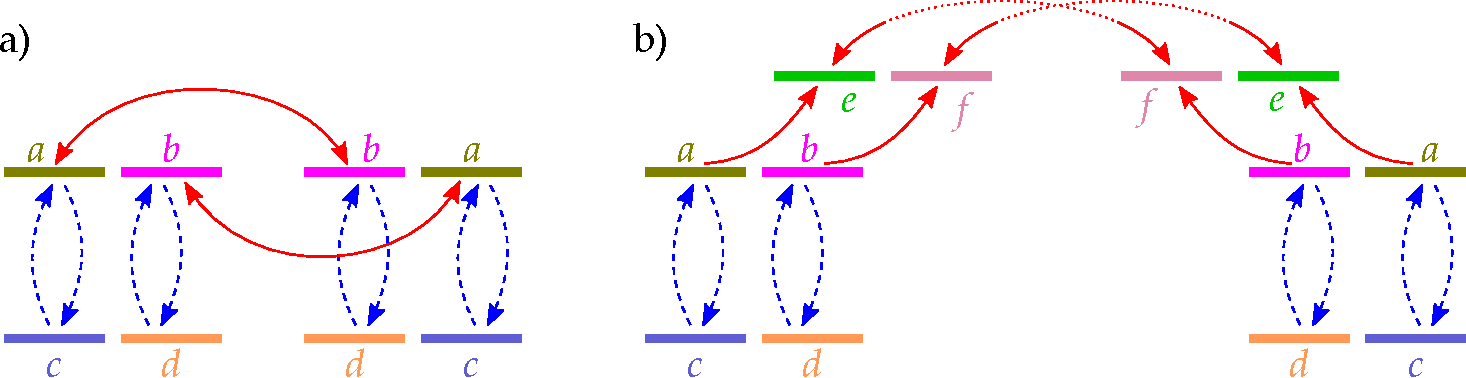
\includegraphics[width=0.9\linewidth]{figures/theory/dipole_coupling_abab}
\caption[Couplage dipolaire entre niveaux de Rydberg différents]{Schéma du couplage dipolaire entre deux atomes dans des niveaux de Rydberg différents $a$ et $b$ : le couplage $ab-ab$ s'effectue au second ordre \textit{via} les niveaux $c$ et $d$. Le couplage $ab-ba$ peut s'effectuer à l'ordre 1(\textbf{a}), à l'ordre 2 via des niveaux intermédiaires $e$ et $f$(\textbf{b}), ou plus encore.}
\label{fig:Dip_abab}
\end{figure}


Lorsque les termes d'échange $A_{ab}$ deviennent comparables aux termes d'interaction directe $C_{ab}$, il peut être judicieux de diagonaliser le hamiltonien effectif \eqref{eq:MatrixCab_Aab}.
En effet, les états propres de celui-ci, qui sont les combinaisons symétrique et anti-symérique $(\ket{ab}\pm \ket{ba})/\sqrt{2}$, ne sont plus dégénérés et présentent respectivement des déplacements d'énergie
\begin{equation}
\label{eq:shift_abab}
\Delta E_{dd} /h = C_{ab} \mp A_{ab}.
\end{equation}

Afin d'illustrer la discussion des interactions que nous venons de présenter, nous allons les appliquer à nos deux exemples que sont le niveau 60S et le niveau 50C.
Dans les deux cas, le calcul numérique consiste à diagonaliser le hamiltonien \eqref{eq:hamilt2atoms} à tous les ordres perturbatifs, en limitant l'espace de Hilbert à quelques centaines d'états de paire et en traitant la distance interatomique de façon classique.

\subsection{Les interactions dipolaires du niveau 60S}\label{subsec:inter_60Snl}

\subsubsection*{L'interaction 60S-60S}
Dans le cas de l'état $\ket{60\text{S},60\text{S}}$, le terme dominant dans la somme \eqref{eq:VdW_aacd} permettant de calculer le coefficient de van der Waals $C_{6,\text{60S60S}}$ est le coulage avec les paires $\ket{60\text{P}_j,59\text{P}_j}$.
Puisque $E_{60S}-E_{59P}>E_{60P}-E_{60S}$, le dénominateur du terme de couplage principal dans \eqref{eq:VdW_aacd} est positif.
On en déduit que l'interaction 60S-60S, et plus généralement toute interaction dipolaire nS-nS, est toujours répulsive.
%
\begin{figure}[!h]
\centering
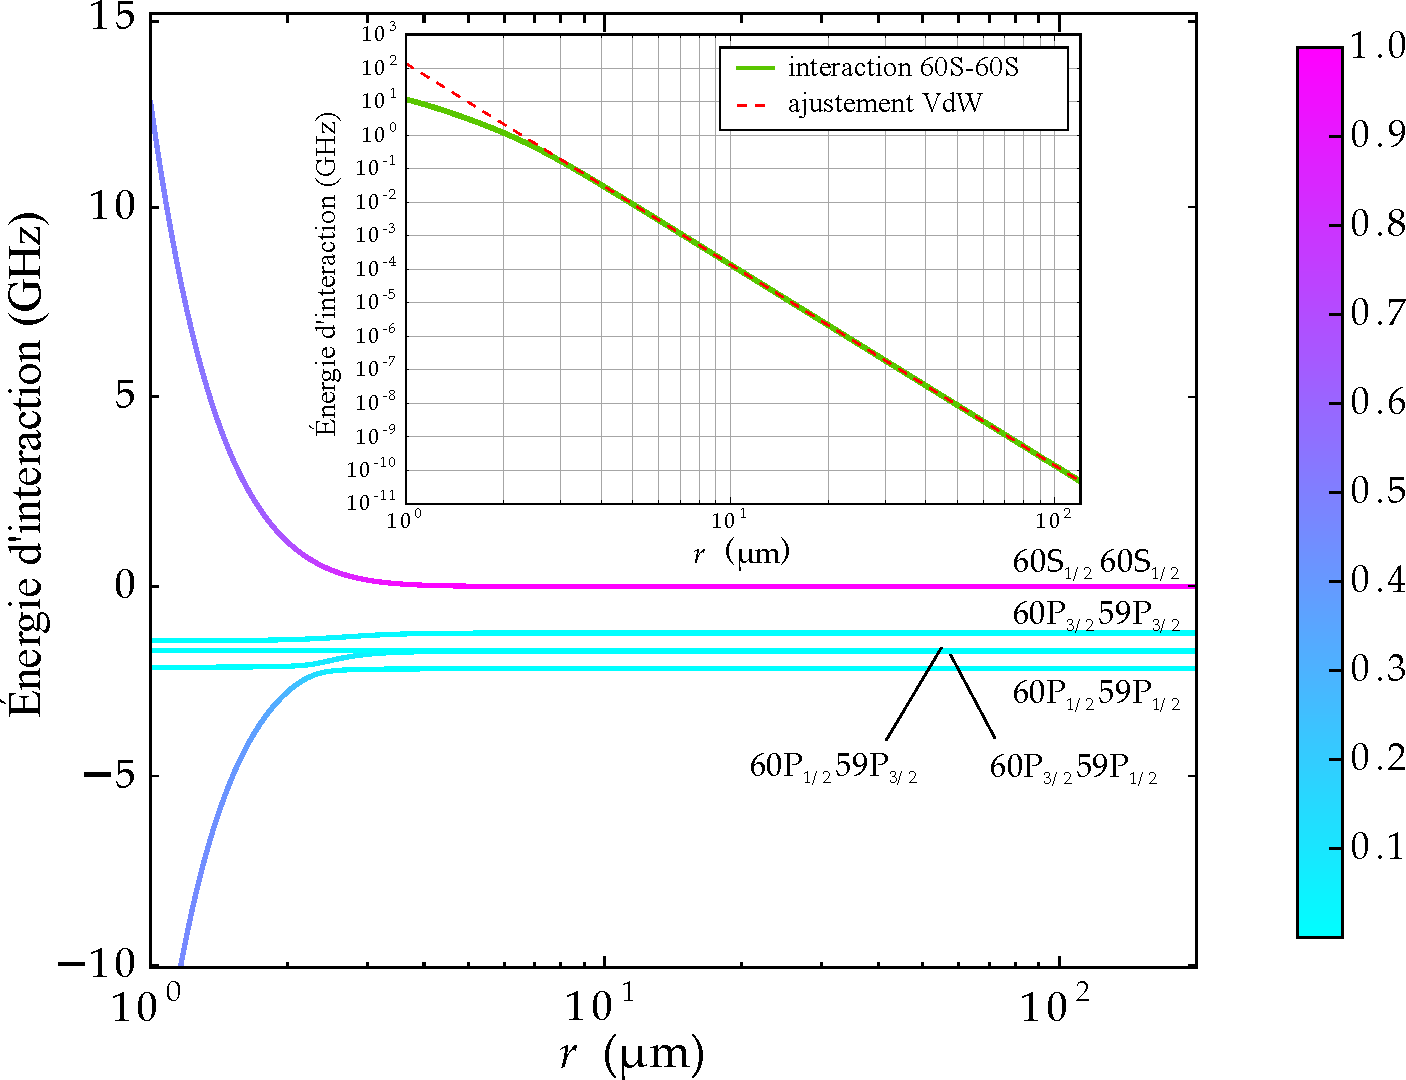
\includegraphics[width=0.8\linewidth]{figures/theory/VdW_60S60S}
\caption[Interaction dipolaire 60S-60S]{Déplacement en énergie de la paire 60S-60S par interaction de van der Waals. Les différents sous-niveaux $\ket{60\text{P}_j,59\text{P}_j}$ sont représentés. L'échelle de couleur représente le carré de la projection sur l'état non perturbé $\ket{60\text{S},60\text{S}}$.
L'insert représente le déplacement d'énergie en échelle log-log et son ajustement sous la forme de van der Waals.}
\label{fig:VdW_60s60s}
\end{figure}
%
Le calcul numérique de l'interaction 60S-60S et son ajustement sous la forme de van der Waals, représentés en figure \eqref{fig:VdW_60s60s}, donnent la valeur
\begin{equation}
\label{eq:C660S}
C_{6,60S60S} = \numv{137.6(1)}\si{\giga\hertz\raiseto{6}\micro\meter}.
\end{equation}

L'ajustement de van der Waals fonctionne très bien aux distances supérieures à $\sim\SIvv{3}{ \micro\meter}$.
Cependant, aux très courtes distances, la paire $\ket{60\text{S},60\text{S}}$ est très fortement couplée aux niveaux $\ket{60\text{P}_j,59\text{P}_j}$.
La distance critique est celle à laquelle le couplage dipolaire est aussi fort que la différence d'énergie entre les deux états de paire non perturbés, soit ici $\sim \SIv{2}{\giga\hertz}$.
En deçà de cette distance, les états propres du hamiltonien s'éloignent de plus en plus de l'état non perturbé $\ket{60\text{S},60\text{S}}$ et l'interaction évolue vers une interaction dipolaire résonante en $1/r^3$.

\subsubsection*{Les interactions 60S-$nl$}
Le niveau 60S interagit également avec des états de $n$ et $l$ différents.
Il convient alors, comme nous l'avons montré en \eqref{subsec:interaction_diff_levels}, de calculer non seulement les coefficients de van der Waals $C_{ab}$, mais aussi les éléments de matrice d'échange $A_{ab}$.
De plus, il est possible ici d'avoir des termes d'échange dûs à un couplage dipolaire direct et qui varient donc en $r^3$.

\begin{figure}[!h]
\centering
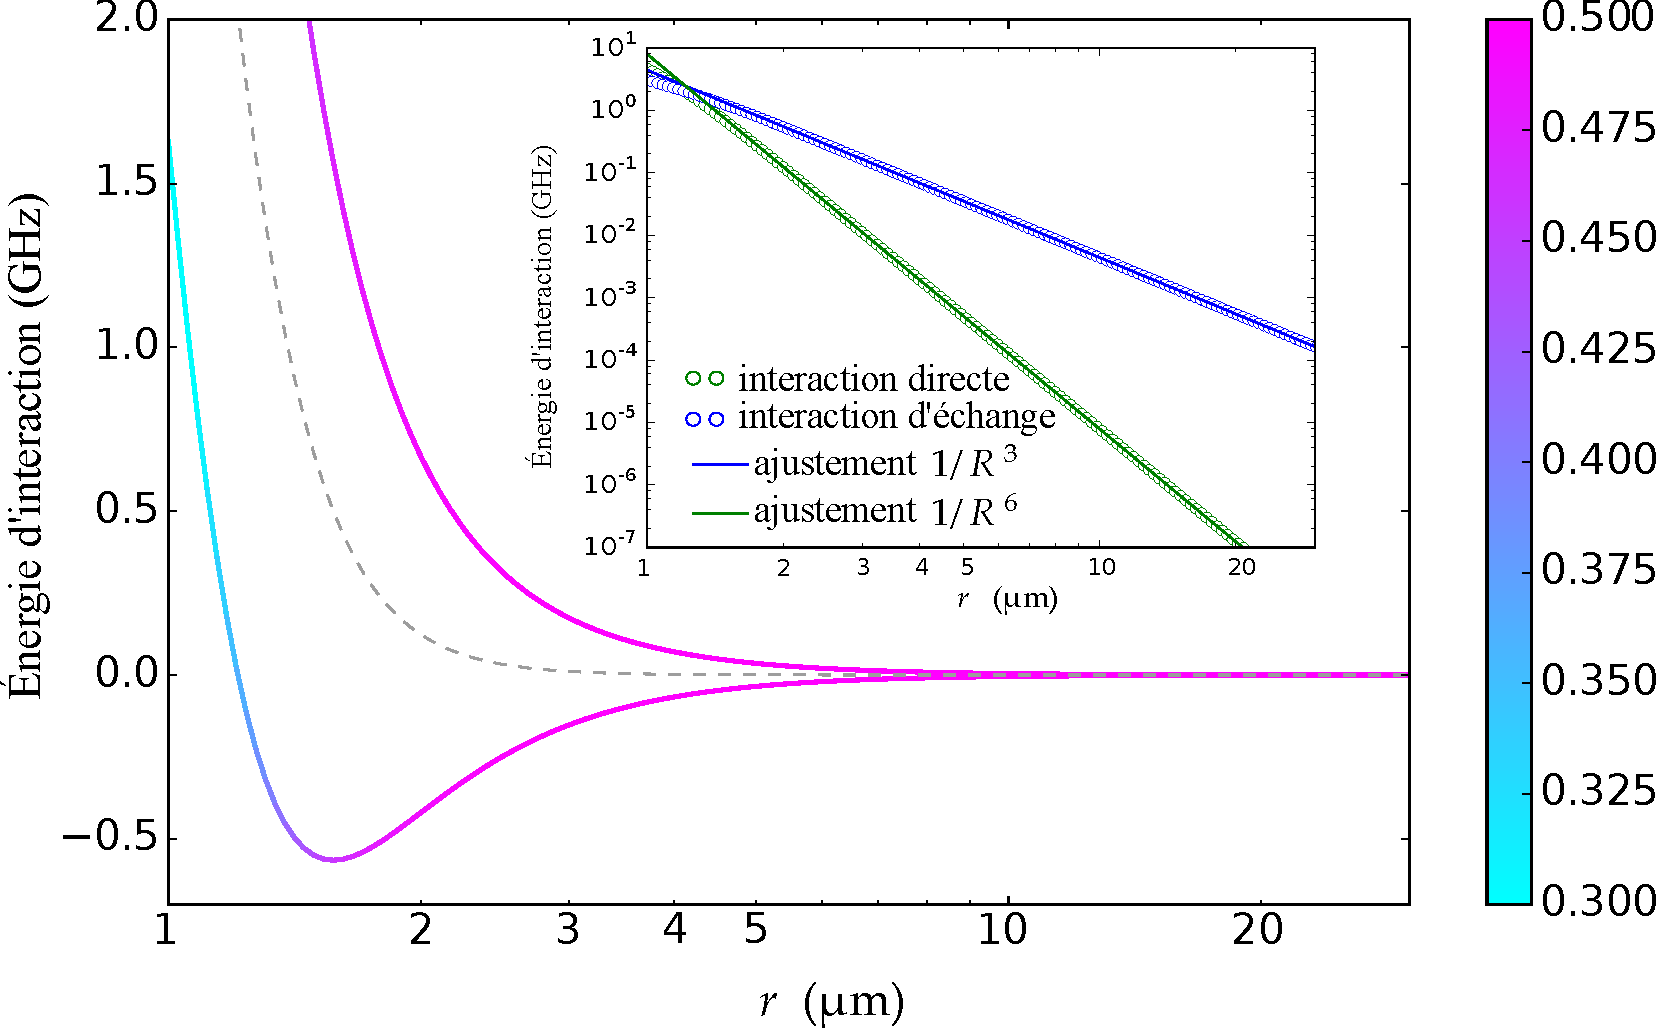
\includegraphics[width=0.8\linewidth]{figures/theory/VdW_60S60P}
\caption[Interaction dipolaire 60S-60P$_{3/2}$]{Énergie de la paire 60S-60P$_{3/2}$ en présence de l'interaction dipolaire.
Les branches inférieure et supérieure correspondent respectivement aux superpositions symétrique et antisymétrique des deux niveaux de départ.
L'échelle de couleur représente le carré de la projection sur l'état non perturbé $\ket{60\text{S},60\text{P}_{3/2}}$.
La ligne pointillée représente le déplacement en énergie dû à l'interaction directe.
L'insert représente le déplacement d'énergie ainsi que le terme d'échange en échelle log-log et leurs ajustements en $1/r^6$ et $1/r^3$ respectivement.
}
\label{fig:VdW_60S60P}
\end{figure}

La figure \eqref{fig:VdW_60S60P} montre par exemple le résultat du calcul de l'interaction dipolaire pour une paire 60S-60P$_{3/2}$.
Aux grandes distances, l'état de la paire est projeté uniformément sur les deux superpositions symétrique et anti-symétrique.
Aux plus courtes distances cependant, d'autres niveaux contaminent la paire, qui n'est plus dans une superposition de $\ket{60\text{S}}$ et $\ket{60\text{P}_{3/2}}$.

En procédant dela même façon, on peut obtenir les coefficients d'interaction dipolaire pour n'importe quelle paire 60S-$nl$. La table \eqref{tab:VdWcoef_60S_nl} synthétise les résultats des calculs numériques pour plusieurs paires contenant le niveau 60S.

\begin{table}[!h]
	\centering
	\caption[Coefficients de van der Waals 60S-nl]{Coefficients de van der Waals pour les interactions de paire entre le niveau 60S et différents niveaux voisins $nl$.}
	\label{tab:VdWcoef_60S_nl}
	\begin{tabular}{c c c c}
		\toprule\midrule
%		\multicolumn{1}{c}{  }
%		&\multicolumn{1}{c}{\text{temps de vie à }\numv{0}\si{\kelvin}}
%		&\multicolumn{1}{c}{\text{temps de vie à }\numv{4.2}\si{\kelvin}}
%		&\multicolumn{1}{c}{\text{temps de vie à }\numv{300}\si{\kelvin}}
%		\\ 
		{ }&$C_6$ (\si{\giga\hertz\raiseto{6}\micro\meter}) & $A_6$ (\si{\giga\hertz\raiseto{6}\micro\meter}) & $A_3$ (\si{\giga\hertz\raiseto{3}\micro\meter})
		\\
		\midrule
		$60\text{S}_{1/2}, 60\text{S}_{1/2}$
		&$\SIv{137.6}{}$
		&$\SIv{0}{}$
		&$\SIv{0}{}$\\
		$60\text{S}_{1/2}, 57\text{S}_{1/2}$
		&$\SIv{-43.265}{}$
		&$\SIv{0.325}{}$
		&$\SIv{0}{}$\\
		$60\text{S}_{1/2}, 61\text{S}_{1/2}$
		&$\SIv{290.125}{}$
		&$\SIv{246.475}{}$
		&$\SIv{0}{}$\\
		$60\text{S}_{1/2}, 60\text{P}_{3/2}$
		&$\SIv{7.976}{}$
		&$\SIv{0}{}$
		&$\SIv{4.411}{}$\\
		\midrule
		\bottomrule
 	\end{tabular}
\end{table}



\subsection{Les interactions dipolaires du niveau 50C}\label{subsec:interac50C_I}
	
\noindent L'interaction dipolaire entre atomes de Rydberg de très grand moment cinétique est rendue plus complexe du fait de leur forte anisotropie.
En effet, l'interaction entre deux dipôles dépend de l'orientation relative de ceux-ci.
Dans le cas des niveaux $l=0$ tel que le 60S, le problème ne se posait pas car ces niveaux sont à symétrie sphérique.
Dès lors que l'on s'intéresse à l'interaction entre des niveaux à symétrie cylindrique, il est indispensable de savoir comment les atomes s'orientent l'un par rapport à l'autre.
L'interaction dipolaire entre atomes circulaires est encore compliquée par l'introduction d'un champ électrique extérieur, qui déplace et déforme les niveaux par effet Stark.
Le détail de l'interaction dipolaire entre atomes circulaires en présence d'un champ sera discuté au chapitre \ref{chapter:circsim}, mais nous prendrons le temps ici de développer la situation la plus simple :
celle de deux atomes dans le niveau 50C dont les deux orbites sont contenues dans le même plan, comme l'illustre la figure \eqref{fig:double_torus}.
%
\begin{figure}[!h]
\centering
\vspace{1em}
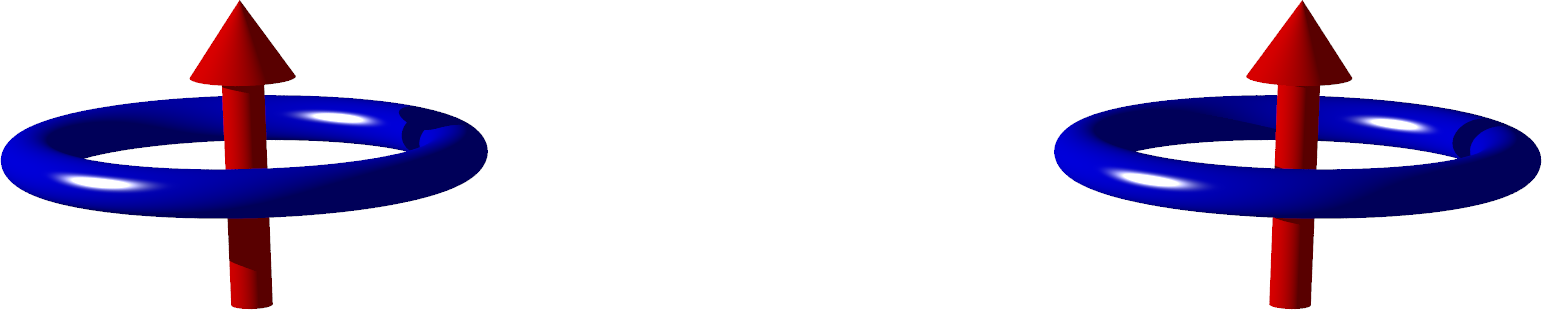
\includegraphics[width=.8\linewidth]{figures/theory/double_torus.png}
\caption[Deux atomes circulaires côte à côte]{Représentation de deux atomes de Rydberg circulaires dont les orbites sont dans le même plan.
Les tores bleus représentent les orbites électroniques et les flèches rouges la direction du moment cinétique.
Si l'on imagine que le dessin est à l'échelle, alors les atomes sont ici séparés d'une distance d'environ \SIv{660}{\nm}.}
\label{fig:double_torus}
\end{figure}
%
Comme il a été dit en \ref{sec:circ_parabol}, les atomes de Rydberg circulaires ont besoin d'un champ électrique extérieur pour se stabiliser.
Nous imposerons donc un champ de \SIvvSym{1}{\V\per\cm}, qui définit l'axe de quantification, parallèle aux flèches rouges sur la figure \eqref{fig:double_torus}.

Les règles de sélection étant toujours valides, le couplage se fait \textit{a priori} à l'ordre deux, et l'équation \eqref{eq:VdW_aacd} permet d'en extraire le coefficient de van der Waals comme nous l'avons fait pour l'interaction 60S-60S.
Cependant, l'équation \eqref{eq:Vdd_rr1r2} ne prend plus la même forme dans la base parabolique et le moment magnétique total $M$ de la paire atomique n'est plus conservé, ce que doit prendre en compte le calcul numérique.

\begin{figure}[!h]
\centering
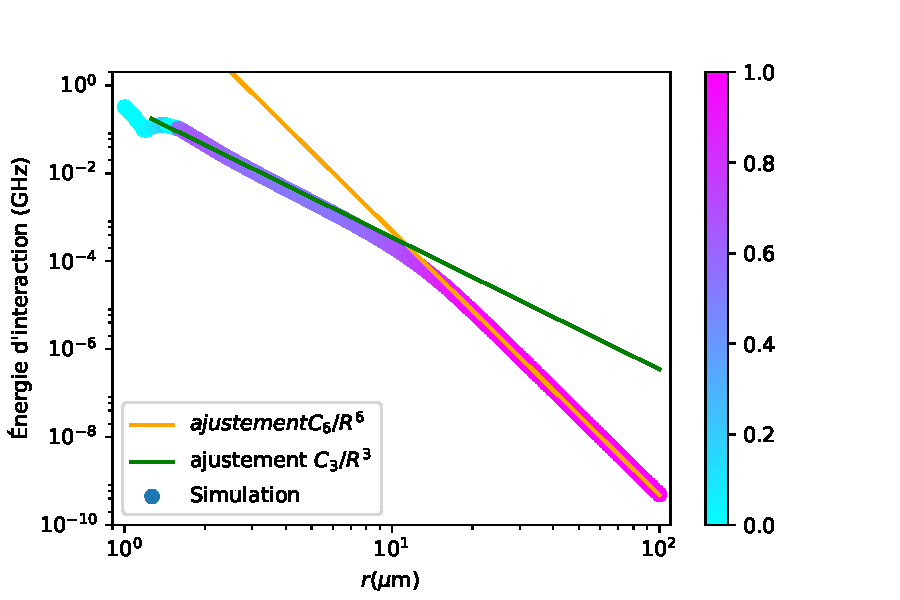
\includegraphics[width=1\linewidth]{figures/theory/VdW_50C50C_1Vcm}
\caption[Interaction dipolaire 50C-50C]{Déplacement en énergie de la paire 50C-50C placés côte à côte (cf fig\eqref{fig:double_torus}) par interaction dipolaire, sous un champ électrique de $\SIvv{1}{\V / \cm}$. L'échelle de couleur représente le carré de la projection sur l'état non perturbé $\ket{50\text{C},50\text{C}}$ de l'état propre du hamiltonien qui le suit adiabatiquement.
Le comportement dévie franchement de la forme de van der Waals en $1/r^6$ dès que la distance interatomique est inférieure à $\SIv{10}{\micro\meter}$.
%Aux très courtes distances, le couplage vers d'autres niveaux atomiques devient très fort et l'énergie d'interaction}
}
\label{fig:VdW_50C50C_1Vcm}
\end{figure}

La figure \eqref{fig:VdW_50C50C_1Vcm} présente le résultat du calcul numérique.
Aux grandes distances, l'énergie d'interaction varie bien en $1/r^6$ comme on l'attend, avec un coefficient de van der Waals 
\begin{equation}
\label{eq:C6_50C50C}
C_{6,50C50C}(\SIvv{1}{V/cm}) = \SI{489.18}{\GHz\raiseto{6}\um}.
\end{equation}
Mais dès que les atomes se rapprochent à une distance inférieure à $\SIvv{10}{\um}$, l'énergie d'interaction varie en $1/r^3$ jusqu'à très courte distance.
En effet, lorsque l'interaction dipolaire devient suffisamment forte, le champ électrique extérieur ne suffit plus à définir le plan des orbites, et le niveau de paire est perturbé.
C'est ce que l'on retrouve sur la coloration de la courbe : à une distance critique de l'ordre de $\SIvv{10}{\um}$ le niveau de la paire s'éloigne du niveau non perturbé $\ket{\mathrm{50C,50C}}$.
La paire est alors dans un état superposé de plusieurs $\ket{nmk,n'm'k'}$, entre lesquels apparaissent des couplages dipolaires résonants en $1/r^3$.
Ce problème sera traité en détail dans le chapitre \ref{chapter:circsim}, lorsque nous nous intéresserons aux conditions dans lesquelles les interactions entre atomes circulaires sont les plus avantageuses pour la simulation quantique.

Si l'on approche encore les deux atomes, à des distances inférieures à \SIvv{2}{\um}, la base des états propres du hamiltonien de paire devient très différente de la base des états non perturbés.
Il est alors très difficile de décrire simplement l'interaction dipolaire.

\section*{Conclusion}
\noindent Nous avons dans ce chapitre présenté les caractéristiques physiques principales des atomes de Rydberg alcalins.
Nous avons utilisé la théorie du défaut quantique afin de décrire les niveaux de Rydberg de faible moment cinétique.
Ceux-ci dévient en effet du modèle de l'atome d'hydrogène par les effets de pénétration et de polarisabilité du c\oe ur atomique, ce que permet de corriger le défaut quantique.
Ainsi nous avons pu décrire le niveau 60S, en donnant la forme de sa fonction d'onde, sa taille et sa durée de vie radiative à différentes températures.

Nous nous sommes ensuite intéressés aux niveaux de Rydberg circulaires, qui semblent être de meilleurs candidats pour la simulation quantique grâce à leur temps de vie plus long.
La théorie du défaut quantique n'est plus nécessaire pour décrire les niveaux circulaires.
Cependant, l'introduction de la base des états paraboliques est d'une grande aide à leur description, en particulier en présence d'un champ électrique.
Nous avons ainsi pu décrire le niveau de Rydberg circulaire 50C, qui présente un temps de vie à température nulle de presque \SIvv{30}{\ms}.

En dernier lieu, nous avons vu comment les atomes de Rydberg interagissent entre eux par interaction dipolaire.
\`A grande distance, l'interaction dipolaire entre deux atomes de Rydberg prend la forme de van der Waals avec une dépendance en $C_6/r^6$, où $r$ est la distance entre les deux atomes.
Nous avons pu déterminer les coefficients de van der Waals $C_6$ pour l'interaction entre une paire d'atomes dans les niveaux $\ket{\text{60S,60S}}$, $\ket{\text{60S,nl}}$ et $\ket{\text{50C,50C}}$, en diagonalisant à chaque fois le hamiltonien complet du système pour toutes les distances $r$.
Aux distances très courtes, lorsque l'interaction dipolaire devient comparable aux différences d'énergie entre les niveaux de Rydberg, les niveaux de Rydberg se mélangent et l'interaction dipolaire ne peut plus être traitée simplement.

Les expériences que nous avons menées portent sur l'étude de l'interaction dipolaire entre atomes de Rydberg.
Il nous a fallu pour cela mettre en \oe uvre un dispositif expérimental que nous présentons dans le prochain chapitre.% \eqref{chapter:setup_coldatoms_Rydberg} .

%Plus particulièrement, nous avons étudié l'interaction dipolaire au sein d'un nuage dense d'atomes dans le niveau 60S, et nous avons 

%Les particularités de l'interaction dipolaire entre niveaux de très grand $l$ sera traitée au chapite \ref{chapter:circsim}.
%\chapter{Atomes de Rydberg alcalins en interaction}
\label{chapter:Rydberg}
%Atomes de Rydberg : à bas $l$ ou circulaires

Un atome de Rydberg est un atome dont un électron au moins occupe un état de grand nombre quantique principal $n$.
Par là, un atome de Rydberg présente des propriétés physiques exacerbées par rapport à un atome non excité ou peu excité.
On le remarque tout d'abord sur sa taille : un atome de rubidium dans le niveau $n=110$ a une extension spatiale de l'ordre d'$1 ~\si{\micro\meter}$, vingt mille fois plus grande que le rayon de Bohr, qui représente l'ordre de grandeur caractéristique de la taille d'un atome dans son état fondamental.

Avec un électron à une telle distance du c\oe ur atomique, les atomes de Rydberg présentent de très grands moments dipolaires de transition entre états de Rydberg voisins. On comprend dès lors leur très grande sensibilité au rayonnement électromagnétique \cite{ENS_ENHANCED}.
Ces très grands moments dipolaires de transition engendrent également de très forts couplages entre atomes de Rydberg voisins, par l'intermédiaire de l'interaction dipolaire. Ces couplages sont eux aussi plusieurs ordres de grandeur plus importants que ceux qui se manifestent entre des atomes dans le niveau fondamental.
L'interaction dipolaire entre atomes de Rydberg est au c\oe ur des travaux de recherche présentés dans cette thèse. Ce premier chapitre vise à en apporter les éléments théoriques importants pour la compréhension des résultats et discussions qui seront abordés par la suite.

La première partie de ce chapitre décrit la théorie du défaut quantique \cite{TXT_GALLAGHER}, qui permet de calculer les énergies propres des états de Rydberg et leur fonction d'onde radiale loin du c\oe ur atomique positif.
Il est alors aisé de calculer les éléments de matrice de l'opérateur de dipôle électrique entre deux niveaux de Rydberg.
Connaître les dipôles de transition entre un niveau de Rydberg et les niveaux voisins permet entre autres de calculer la durée de vie des niveaux de Rydberg.
Nous introduirons ensuite la base des états paraboliques qui permet une description claire des niveaux de Rydberg circulaires en présence d'un champ extérieur.
La connaissance des dipôles de transition est également essentielle au calcul des interactions dipolaires entre deux atomes de Rydberg, ce que nous aborderons dans un troisième paragraphe.
Enfin, nous discuterons le détail de cette interaction dans deux cas particuliers  : les atomes de Rydberg en interaction autour du niveau $60$S et les atomes de Rydberg en interaction autour du niveau circulaire $50$C.
Ces deux cas particuliers seront à nouveau discutés plus en détail dans des chapitres dédiés aux expériences que nous avons menées.

\section{Les atomes de Rydberg alcalins : des hydrogénoïdes géants}\label{sec:alkalRydberg}
\noindent Un atome de Rydberg alcalin a un seul électron dans un niveau de grand nombre quantique principal $n$. L'essentiel de la fonction d'onde de cet électron est localisé dans des régions atomiques éloignées du c\oe ur, c'est-à-dire de l'ensemble du noyau atomique et des couches électroniques inférieures.
Pour cette raison, il ressemble à un atome d'hydrogène, dont l'unique électron voit un c\oe ur protonique simple de charge totale $+q=\numv{1.602176565(35)d-19}\si{\coulomb}$ \cite{MX_CODATA14}.
Dans le cas de l'hydrogène, ce c\oe ur est plusieurs ordres de grandeurs plus petit que la taille typique de l'orbite de l'électron : le niveau électronique fondamental $1$S a un \og rayon \fg{} caractéristique $a_0 = \numv{0,52917721092(17)}\si{\angstrom}$ \cite{MX_CODATA14}, alors que le proton a un rayon $r_p = \numv{0.8775(51)}\si{\femto\meter}$ \cite{MX_CODATA14}.

Les cinq ordres de grandeur séparant le rayon de l'orbite électronique et le rayon du proton permettent de considérer que le potentiel vu par l'électron est parfaitement coulombien sur tout l'espace.
Les énergies propres de l'atome d'hydrogène sont alors données par
\begin{equation}\label{eq:Hatom}
E(n,l,j)= - \frac{E_I}{n^2} ,
\end{equation}

avec
\begin{equation}\label{eq:E_I}
E_I = \frac{1}{1+\frac{m_e}{M}}\frac{m_e q^4}{32\pi^2 \epsilon _0^2 \hbar ^2}
\end{equation}
l'énergie d'ionisation pour l'électron dans le niveau $1$S de l'atome d'hydrogène, où $M$ est la masse du c\oe ur atomique (masse d'un proton pour l'atome d'hydrogène, masse atomique $m_{Rb87}$ pour l'atome de $^{87}Rb$ dans un état de Rydberg), $n$ le nombre quantique principal, $m_e$ la masse de l'électron, $\epsilon_0$ la permittivité diélectrique du vide, et $\hbar$ la constante de Planck réduite.

Les états propres de ce modèle s'écrivent en coordonnées sphériques comme le produit d'une partie radiale, fonction de $r$ qui est la distance de l'électron au c\oe ur atomique, par une partie angulaire, fonction des coordonnées angulaires $\theta$ et $\phi$ \cite{TXT_COHEN1FR} : 
\begin{equation}\label{eq:Hfonctonde}
\psi(r,\theta,\phi) = R_{nl}(r)\cdot Y_l^{m_l}(\theta,\phi).
\end{equation}
Ici, $l$ est le nombre quantique orbital et $m_l$ le nombre quantique magnétique, associé à la projection du moment angulaire orbital de l'électron sur l'axe de quantification.
Cette première description ne prend pas en compte les corrections aux énergies dues au couplage entre le moment magnétique intrinsèque de l'électron, son spin, et son moment magnétique orbital correspondant à la structure fine.
Elle néglige tout autant le couplage entre le moment magnétique total de l'électron et le moment magnétique du c\oe ur atomique, le couplage hyperfin \cite{TXT_COHEN2FR}.

Là où la structure fine est importante, les bons nombres quantiques deviennent $n,l,j,m_j$, avec $j=l+s$ où $s=1/2$ est le moment magnétique de spin de l'électron. Le couplage hyperfin étant très petit pour les niveaux de Rydberg, nous en ferons fi et continuerons d'utiliser la base avec moment cinétique total $j$ de l'électron pour décrire les niveaux électroniques.

En comparaison avec l'atome d'hydrogène, le c\oe ur positif de l'atome de Rydberg alcalin comporte une structure d'extension spatiale bien plus importante \cite{TXT_GALLAGHER}.
Dans la région des couches électroniques inférieures, le potentiel est bien plus profond que le potentiel coulombien car l'effet d'écrantage partiel de la charge totale positive du c\oe ur par les électrons internes disparaît lorsque l'on s'en approche : c'est l'effet de pénétration du c\oe ur.
Par ailleurs, la distribution spatiale des charges positives et négatives entraîne une polarisabilité du c\oe ur composé.
L'électron de Rydberg interagit avec cette distribution de charge complexe, ce qui modifie sa fonction d'onde et son énergie propre.
Afin de rendre compte de ces effets, il est nécessaire d'apporter une correction aux énergies propres de l'électron de Rydberg d'un atome alcalin : le défaut quantique.

	\subsection{Hamiltonien de l'atome de Rydberg et défaut quantique}
\noindent Les deux effets précédemment cités de pénétration du c\oe ur et de polarisabilité du c\oe ur peuvent être efficacement décrits par la théorie du défaut quantique. Celui-ci apparaît comme une correction $\delta_{nlj}$ au nombre quantique principal $n$ dans l'équation des énergies propres des niveaux électroniques \cite{TXT_GALLAGHER}, qui devient
\begin{equation}\label{eq:E_I_delta}
E(n,l,j) = \frac{- E_I}{(n-\delta_{nlj})^2} ,
\end{equation}
avec 
\begin{equation}\label{eq:deltanlj}
\delta(n,l,j)=\delta_{lj,0} + \frac{\delta_{lj,2}}{(n-\delta_{lj0})^2} + \frac{\delta_{lj,4}}{(n-\delta_{lj0})^4} + \frac{\delta_{lj,6}}{(n-\delta_{lj0})^6} + \cdots .
\end{equation}

\begin{table}[tph!]
	\centering
	\caption[Défauts quantiques du $^{87}Rb$ et $^{85}Rb$]{Défauts quantiques  du \Rb{85} extraits de \cite{MX_GALLAGHERSPECRBNSND03, MX_GALLAGHERSPECRBNF06} et du \Rb{87} extraits de \cite{MX_MACKNSNDRYD}}
	\label{tab:q_defect}
	\begin{tabular}{ c S[table-format=1.12]S[table-format=2.8]  S[table-format=1.10]S[table-format=2.6]}
		\toprule\midrule
		 &  \multicolumn{2}{c}{\Rb{85}}	&   \multicolumn{2}{c}{\Rb{87}}  \\ 
		 \midrule
				  &		$\delta_{lj,0}$				&	$\delta_{lj,2}$		&	$\delta_{lj,0}$			&	$\delta_{lj,2}$ \\ 
		\midrule
		$nS_{1/2}$&  	3.1311804(10)		&	0.1784(6) 	& 3.1311807(8)	& 0.1787(2)	\\
		$nP_{1/2}$&  	2.6548849(10)		&	0.2900(6)	&						&				\\
		$nP_{3/2}$&  	2.6416737(10)		&	0.2950(7)	&						&				\\
		$nD_{3/2}$&  	1.34809171(40)	&	-0.60286(26)&1.3480918(11)	&	-0.6054(4)	\\
		$nD_{5/2}$&  	1.34646572(30)	&	-0.59600(18)&1.3464622(11)	&-0.5940(4)		\\
		$nF_{5/2}$&  	0.0165192(9)		&	-0.085(9)	&						&				\\
		$nF_{7/2}$&  	0.0165437(7)		&	-0.086(7)	&						&				\\
%		$nG$	&0.00400(9)	&&&\\
%		$n,l>4$ & {$0.004(4/l)^5$}&&&\\
		\midrule
		\bottomrule
 	\end{tabular}
\end{table}
%
La série \eqref{eq:deltanlj} développe le défaut quantique en puissances de $1/(n-\delta_{lj,0}) = 1/n^*$ : $n^*$ est le nombre quantique principal corrigé du défaut quantique.
Ses coefficients, présentés en table \eqref{tab:q_defect}, sont extraits des mesures précises des fréquences de transition entre niveaux de Rydberg voisins \cite{ENS_SPECNA2,ENS_SPECCS,MX_MECHEDERYDSPECTRO87} et la série sous cette forme converge rapidement \cite{MX_MARTINSERIESSPECNA} :
pour les niveaux de $n>40$, les deux premiers termes suffisent à obtenir une précision meilleure que la centaine de $\si{\kilo\hertz}$ sur une large gamme de valeurs de $n$.
Les coefficients de la série sont fonction de $l$ et $j$, ainsi que de l'espèce atomique.
Nous n'avons pas connaissance de défauts quantiques mesurés pour le \Rb{87} autres que ceux présentés ici, mais l'utilisation de ceux du \Rb{85} fournit de bons résultats grâce à la grande similarité des structures électroniques de ces deux isotopes.
En ce qui concerne les niveaux de $l>3$, leurs défauts quantiques sont petits, et donc d'autant plus difficiles à mesurer. Ils seront donc négligés par la suite.
Avec les valeurs connues des défauts quantiques, nous obtenons des fréquences de transition entre niveaux de Rydberg voisins avec une précision meilleure que $\sim 50\si{\kilo\hertz}$.

Dans le cas extrême des niveaux de Rydberg circulaires, qui ont un moment orbital maximal $l=n-1$, le défaut quantique peut être considéré nul et alors on retrouve le modèle de l'atome d'hydrogène sans correction autre que la masse du c\oe ur.
		
	\subsection{Partie radiale de la fonction d'onde et calcul du dipôle de transition}
\noindent Ayant ces outils à notre disposition, nous pouvons désormais nous employer à calculer les éléments de matrice de l'opérateur de transition dipolaire $\vec{d}=q\vec{r}$ entre niveaux de Rydberg, qui apparaît de façon essentielle dans les termes de couplage des atomes avec le rayonnement électromagnétique et dans le couplage dipolaire entre deux niveaux de Rydberg $\ket{n,l,j,m_j}$ et $\ket{n',l',j',m_j'}$. Ces éléments de matrice s'écrivent

	\begin{equation}\label{eq:matrixelements}
	\begin{aligned}
	\bra{nl,l,j,m_j}q\vec{r}\ket{n',l',j',m_j'}= & ~q\bra{n,l,j,m_j} r\frac{\vec{r}}{r} \ket{n',l',j',m_j'} \\
	= & ~q\cdot \int r^2dr~R^*_{nl}(r)~r~R_{n',l'}(r)~ \bra{l,j,m_j}\frac{\vec{r}}{r}\ket{l',j',m_j'} \\
	= & ~q.\mathcal{R}(nl,n'l').\mathcal{A}(ljm_j,l'j'm_j')	 ,
	\end{aligned}
	\end{equation}
	
\noindent c'est-à-dire comme produit d'une partie radiale $\mathcal{R}$ et d'une partie angulaire $\mathcal{A}$.
Or la partie radiale $R_{n,l}(r)$ de la fonction d'onde est affectée par l'effet de pénétration du c\oe ur décrit plus haut et doit donc être corrigée \cite{TXT_GALLAGHER}.
Le calcul de $\mathcal{R}$ peut être fait numériquement par une méthode dite de Numerov \cite[pp.10-24]{TXT_GALLAGHER}.
Cette méthode s'appuie sur le fait que le potentiel à l'extérieur du c\oe ur atomique reste coulombien.
La partie radiale de la fonction d'onde peut donc y être calculée à partir de la même équation que pour l'atome d'hydrogène, avec les mêmes conditions aux limites à $r \rightarrow \infty$, mais avec une énergie totale différente qui est fixée par les défauts quantiques, et en tronquant à une distance finie du c\oe ur pour éviter la divergence du potentiel à distance nulle.

\begin{figure}[!h]
	\centering
	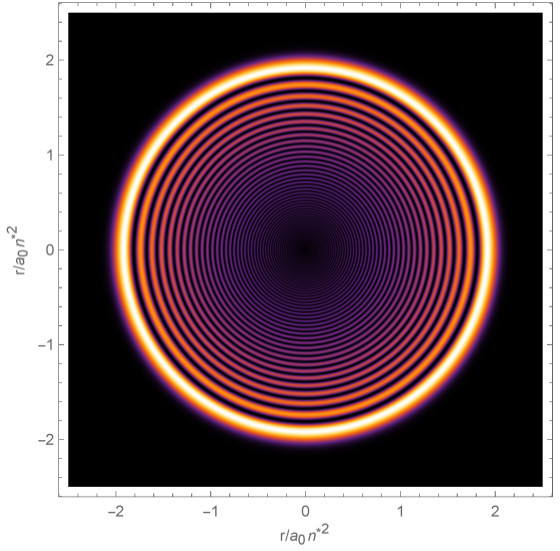
\includegraphics[width=0.6\linewidth]{figures/theory/WaveFunc_60S_}
	\caption[Fonction d'onde du niveau nS]{Probabilité de présence de l'électron dans le niveau nS : $r^2\times |R_{\mathrm{nS}}(r)|^2$, dans l'un quelconque de ses plans de symétrie.}
	\label{fig:wavefunc60S}
\end{figure}

La figure \eqref{fig:wavefunc60S} montre la probabilité de présence $r^2|R_{\mathrm{nS}}(r)|^2$ de l'électron de Rydberg dans le niveau nS du \Rb{87}.
Cela montre que la fonction d'onde se situe essentiellement loin du c\oe ur atomique et justifie donc la validité de la méthode de Numerov.

\`A partir du calcul de $R_{nl}(r)$, l'on peut aisément dériver la partie radiale de l'opérateur dipôle $\vec{d}$.
L'on apprend en particulier que la partie radiale de $\vec{d}$ entre deux niveaux de nombre quantique principal similaire varie comme $\mathcal{R} \sim a_0\cdot n^{*2}$.
Mentionnons ici que le rayon moyen de l'orbitale électronique d'un niveau de Rydberg est très similaire au calcul de la partie radiale de l'opérateur dipôle :
\begin{equation}\label{eq:orbital_size}
\braket{r_{\ket{n,l,j,m_j}}} = \int r^2dr~R_{nl}(r).r.R_{nl}(r) = \mathcal{R}(nl,nl) \propto a_0 \cdot n^{*2}.
\end{equation}
%\`A titre d'exemple, le niveau $60$S a ainsi un rayon moyen de $\braket{r} = 4850~a_0 = \numv{256.5}~\si{\nano\meter}$.
\`A titre d'exemple, l'équation \eqref{eq:orbital_size} permet d'obtenir la taille de l'orbitale électronique dans le niveau $\mathrm{60S_{1/2}}$ : son rayon moyen vaut $\braket{r} = 4850~a_0 = \numv{256.5}\si{\nano\meter}$.

	\subsection{L'effet Stark}\label{sec:Stark}
\noindent Les atomes de Rydberg étant très sensibles au champ électrique, il est important de comprendre comment celui-ci agit.
%Afin de comprendre ce phénomène plus en détail, attardons-nous à décrire l'effet Stark.
La présence d'un champ électrique constant $\vec{F}$ dans l'environnement ajoute au hamiltonien atomique un terme de couplage \og Stark \fg{}  entre le champ et l'opérateur dipolaire électrique.
En présence d'un champ électrique, le hamiltonien devient
\begin{equation}
\label{eq:hamilt_Stark}
\hat{H} = \hat{H}_0 - \vec{\hat{d} \cdot F} = \hat{H}_0 + q~\vec{\hat{r}\cdot F},
\end{equation}
où $\hat{H}_0$ est le hamiltonien libre de l'atome, dont les énergies propres sont calculées par la théorie du défaut quantique selon l'équation \eqref{eq:E_I_delta}, $\hat{\vec{r}}$ l'opérateur position de l'électron dans le potentiel atomique et $q$ la charge élémentaire, supposée positive.

Le hamiltonien Stark \eqref{eq:hamilt_Stark} perd la symétrie sphérique de $\hat{H}_0$, au profit d'une symétrie cylindrique autour de l'axe défini par le vecteur de champ électrique $\vec{F}$.
Cet axe, que nous choisirons comme étant l'axe $(Oz)$, devient alors l'axe de quantification naturel du problème.
Dans la base construite autour de cet axe, le terme d'énergie Stark prend la forme
\begin{equation}
\label{eq:dipole_Stark}
\hat{H}_S = q\hat{z}|\vec{F}| = q\hat{r} \sqrt{\frac{4\pi}{3}} Y_1^0  |\vec{F}|.
\end{equation}
où $\hat{z}$ est la composante selon $z$ de l'opérateur position, $\hat{r}$ sa norme, et $Y_
1^0$ l'harmonique sphérique $(l=1,m_l=0)$.
Ce hamiltonien ne couple que les états de même $m_l$ et vérifiant $\Delta l = \pm 1$.

Le calcul de l'effet Stark par diagonalisation du hamiltonien pour un niveau de Rydberg donné est alors simple à mener numériquement, en réduisant le sous-espace à considérer grâce à la règle de sélection $\Delta m_l = 0$.
Cette même règle de sélection permet d'imposer la condition $\Delta m_j= \Delta m_l + \Delta m_s = 0$, car l'effet Stark n'introduit aucun terme permettant de coupler des états de spins électroniques différents.
La figure \eqref{fig:Stark_60S} montre les énergies propres trouvées par diagonalisation du hamiltonien \eqref{eq:hamilt_Stark}, pour les états d'énergie proche de celle du niveau $\mathrm{60S_{1/2},m_j=1/2}$ et de même $m_j$.
%
\begin{figure}[!h]
\centering
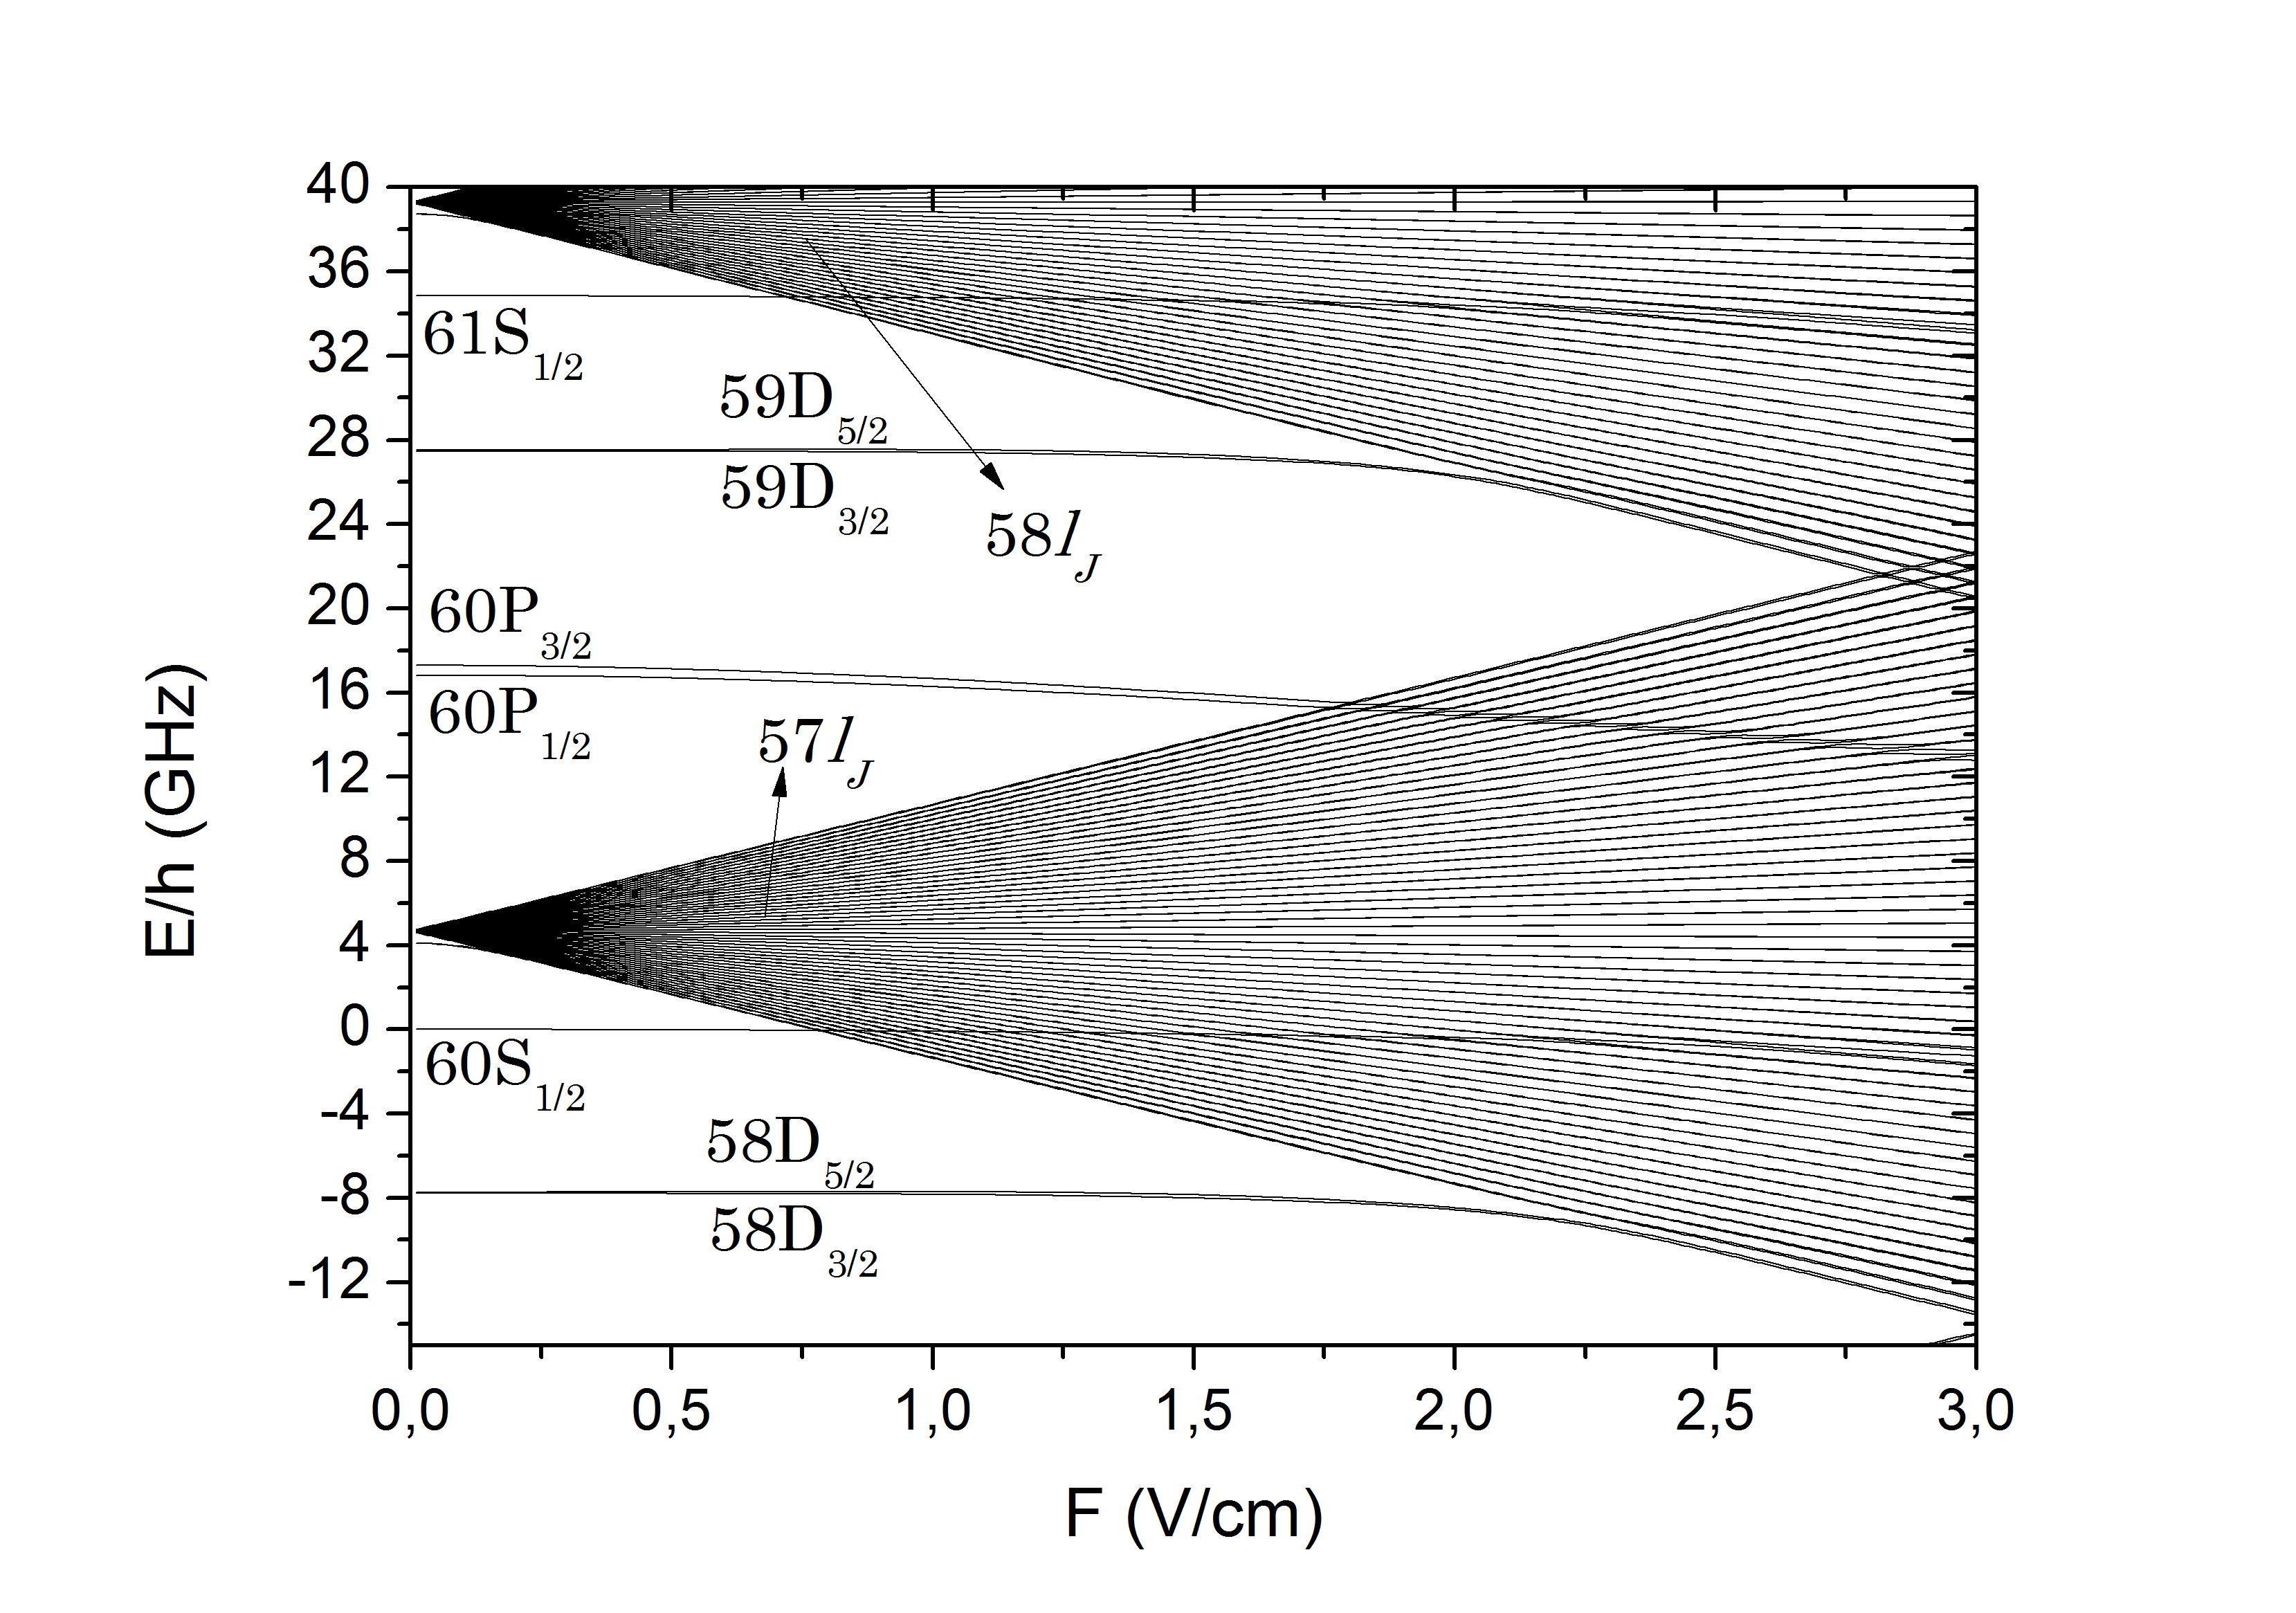
\includegraphics[width=\linewidth]{figures/setup/rydberg/Stark_60S}
\caption[Diagramme Stark autour du niveau $\mathrm{60S}$]{
Diagramme Stark autour du niveau $\mathrm{60S}$, pour les états de $m_j=1/2$.
Le défaut quantique déplace beaucoup les niveaux S,P et D.
Ces niveaux non-dégénérés ont un effet Stark quadratique en champ électrique.
Les niveaux de grand $l$ sont dégénérés et ont un effet Stark linéaire (ce sont les multiplicités qui s'ouvrent en éventail).
}
\label{fig:Stark_60S}
\end{figure}
%
Deux cas sont à distinguer. Les niveaux de faible moment orbital $l\leq 3$ sont déplacés en énergie par leur défaut quantique important.
Le terme d'interaction Stark ne couplant que des niveaux ayant la même énergie en l'absence de champ électrique, ces niveaux S,P et D ne sont perturbés qu'au second ordre par l'effet Stark.
Leur énergie varie donc de façon quadratique avec le champ électrique.
Les niveaux de grand nombre quantique orbital $l$ et de même nombre quantique principal $n$ sont, eux, dégénérés.
Le champ électrique sépare donc leurs énergies linéairement
\footnote{
Le cas de l'effet Stark pour les atomes de grand $l$ sera traité plus en détail dans le chapitre \ref{chapter:circsim}.
}.
La figure \eqref{fig:Stark_60S} montre deux telles multiplicités, $n=57$ et $n=58$.

Les niveaux de bas $l$ présentent donc tous un effet Stark quadratique que l'on exprime sous la forme
\begin{equation}
\label{eq:Stark_quad}
\Delta \nu_S = A\cdot\vec{F}^2.
\end{equation}
%On comprend mieux ainsi la forme des raies présentées en figure \eqref{fig:vieilles_raies} :
%l'effet Stark ne peut que réduire la fréquence de transition $5S-60S$ et la raie n'est donc élargie que du côté des basses fréquences.
%
La diagonalisation du hamiltonien \eqref{eq:hamilt_Stark} et l'ajustement des énergies propres ainsi calculées nous permettent d'extraire les coefficients d'effet Stark pour n'importe quel niveau.
La table \eqref{tab:Stark_60S} répertorie les coefficients d'effet Stark quadratique pour quelques niveaux autour du $\mathrm{60S}$.

\begin{table}[!h]
	\centering
	\caption[Effet Stark quadratique des niveaux proches du $\mathrm{60S}$]{Coefficients d'effet Stark quadratique des niveaux proches du $\mathrm{60S}$.
	}
	\label{tab:Stark_60S}
	\begin{tabular}{c c }
		\toprule\midrule
		Niveau de Rydberg
		& Coefficient Stark quadratique
		\\
		$\ket{n,l,j}$
		& $A_{n,l,j,m_j}$ en $\si{\MHz \per (\V \per\cm) \squared}$ \\
		\midrule
		$\mathrm{60S_{1/2}}$
		& \SI{-89.9}{} \\
		$\mathrm{61S_{1/2}}$
		& \SI{-100.9}{} \\
		$\mathrm{60P_{3/2},m_j=\pm -1/2}$
		& \SI{-676}{} \\
		$\mathrm{60P_{3/2},m_j=\pm -3/2}$
		& \SI{-569}{} \\
		\midrule
		\bottomrule
 	\end{tabular}
\end{table}

%\noindent Si l'on suppose que la largeur des spectres de la figure \eqref{fig:vieilles_raies} est due principalement à l'effet Stark causé par des gradients de champ électrique, alors ceux-ci peuvent s'estimer grâce aux coefficients données en table \eqref{tab:Stark_60S}.
%Une largeur de raie de $\SI{40}{\MHz}$ correspond à un champ électrique variant de $\SIrange{0}{0.667}{\V/\cm}$ sur l'extension du nuage.
%Or le nuage utilisé pour ces spectres était un MOT de $\sim \SI{200}{\um}$ de diamètre, ce qui nous donne une valeur de gradient de champ électrique de l'ordre de $\SI{35}{(\V/\cm)\per\cm}$.

	\subsection{Temps de vie des niveaux de Rydberg}
\noindent Avec la connaissance des dipôles de transition d'un niveau de Rydberg vers les niveaux voisins, 	il est possible de connaître le temps de vie de celui-ci.
Deux processus entrent en jeu dans la désexcitation radiative à température finie de ces niveaux atomiques :
les transitions par émission spontanée mais aussi les transitions par absorption ou émission stimulée par le rayonnement de corps noir de leur environnement.
En effet, les transitions entre niveaux de Rydberg proches en énergie sont dans le domaine des micro-ondes millimétriques.
Cela implique qu'elles seront à considérer dès les très basses températures : contrairement aux photons optiques, des photons micro-ondes sont déjà émis par le rayonnement du corps noir aux températures cryogéniques, de quelques \si{\milli\kelvin} à quelques \si{\kelvin}.

\`A titre d'exemple, la fréquence de la transition entre le niveau $\ket{60\mathrm{S}1/2}$ et le niveau $\ket{59\mathrm{P}3/2}$ vaut $\nu = E/h = \numv{18.5213}\si{\giga\hertz}$. La température de corps noir correspondant à cette fréquence est de $T=h\nu /\kb = \numv{0.89}\si{\kelvin}$.
Cette transition sera donc limitante pour le temps de vie du niveau 60S dès lors que celui-ci sera dans un environnement dépassant les $\numv{500}\si{\milli\kelvin}$.

%Or les températures de rayonnement du corps noir associées à ces gammes de fréquence se situent dans la gamme de quelques \si{\milli\kelvin} à quelques \si{\kelvin}.
\`A température nulle, le temps de vie d'un niveau excité est calculé uniquement à partir des coefficients d'Einstein pour l'émission spontanée \cite{MX_GALLAGHERBBODY}. Un électron dans un niveau excité est couplé aux niveaux de plus basse énergie par les modes électromagnétiques du vide et le taux de désexcitation d'un niveau initial $\ket{i}$ vers un niveau final $\ket{f}$ séparés d'une énergie $E_f - E_i = -\hbar \omega_{if} < 0$ est donné par :
\begin{equation}\label{eq:EinsteinAif}
A_{if} = \frac{2\omega_{if}^3}{3\epsilon_0c^3h}\cdot q^2\cdot |\bra{i}r\ket{f}|^2
\end{equation}
Ce coefficient est le produit de la densité de modes du rayonnement électromagnétique autour de la fréquence résonante $\nu_{if}=\omega_{if}/2\pi$ et du moment dipolaire de transition entre les niveaux $\ket{i}$ et $\ket{f}$ couplés par ce rayonnement.
Le temps de vie de l'état excité est alors calculé en sommant les taux d'émission spontanée vers chacun des niveaux auxquels il a accès par transition dipolaire électrique.
Les transitions dipolaires par émission d'un photon respectant la règle de sélection $\Delta l = \pm1$ et $\Delta m \leq 1$, la quantité de termes à considérer s'en trouve heureusement limitée.

\`A température finie cependant, l'absorption et l'émission stimulée vers les niveaux voisins entrent en jeu.
Le coefficient d'Einstein pour l'absorption et  l'émission stimulée s'écrit ici
\begin{equation}\label{eq:EinsteinBif}
B_{if} = A_{if} . \bar{n}(\omega_{if})
\end{equation}
Il s'agit alors de connaître, pour une température donnée, le taux d'occupation du rayonnement électromagnétique aux fréquences des transitions entre niveaux de Rydberg.
Ce taux nous est donné par la distribution de Bose-Einstein pour un gaz de bosons \cite{TXT_GORECKIPHYSTAT} :
\begin{equation}\label{eq:BoseStat}
\bar{n}(\omega) = \frac{1}{e^{\frac{\hbar\omega}{\kb T}}-1}
\end{equation}
qui devient, lorsque $\kb T \gg \hbar\omega$,
\begin{equation}\label{eq:BoseStat_blackbody}
\bar{n}(\omega) \sim \frac{\kb T}{\hbar\omega}.
\end{equation}
Le nombre de photons par mode varie alors linéairement avec la température et ces photons stimulent des transitions vers des niveaux de Rydberg proches, diminuant ainsi le temps de vie du niveau de départ.


	%\subsection{Le niveau de Rydberg 60S : $\mathbf{\ket{n=60,l=0}}$}
%\noindent Afin d'illustrer les propriétés singulières des niveaux de Rydberg, prenons un exemple qui nous sera utile par la suite : le niveau de Rydberg 60S, qui a donc un moment cinétique orbital $l=0$. Nous nous intéresserons à sa taille, à ses dipôles de transition avec les niveaux voisins, et à son temps de vie.

%Grâce à l'équation \eqref{eq:orbital_size}, nous pouvons obtenir la taille de l'orbitale électronique dans le niveau 60S : son rayon moyen vaut $\braket{r} = 4850~a_0 = \numv{256.5}\si{\nano\meter}$.
%, valeur qui paraît très grande en comparaison avec l'extension spatiale d'un atome dans le niveau fondamental qui est de l'ordre de quelques $a_0$.

\subsubsection*{Temps de vie du niveau $\mathbf{60S_{1/2}}$}
De par la règle de sélection $\Delta l=\pm1$, les termes à considérer pour les transitions dipolaires depuis le niveaux $\ket{n=60,l=0}$ sont les couplages avec les niveaux $n\mathrm{P}_j = \ket{n,l=1,j},~j\in\{1/2,3/2\}$.
La figure \eqref{fig:matrixelements} montre, pour tous les $n$, la somme des coefficients d'Einstein d'émission spontanée et d'absorption et émission stimulée à différentes températures vers les niveaux $n\mathrm{P}_j$.

\begin{figure}[th!]
	\centering
	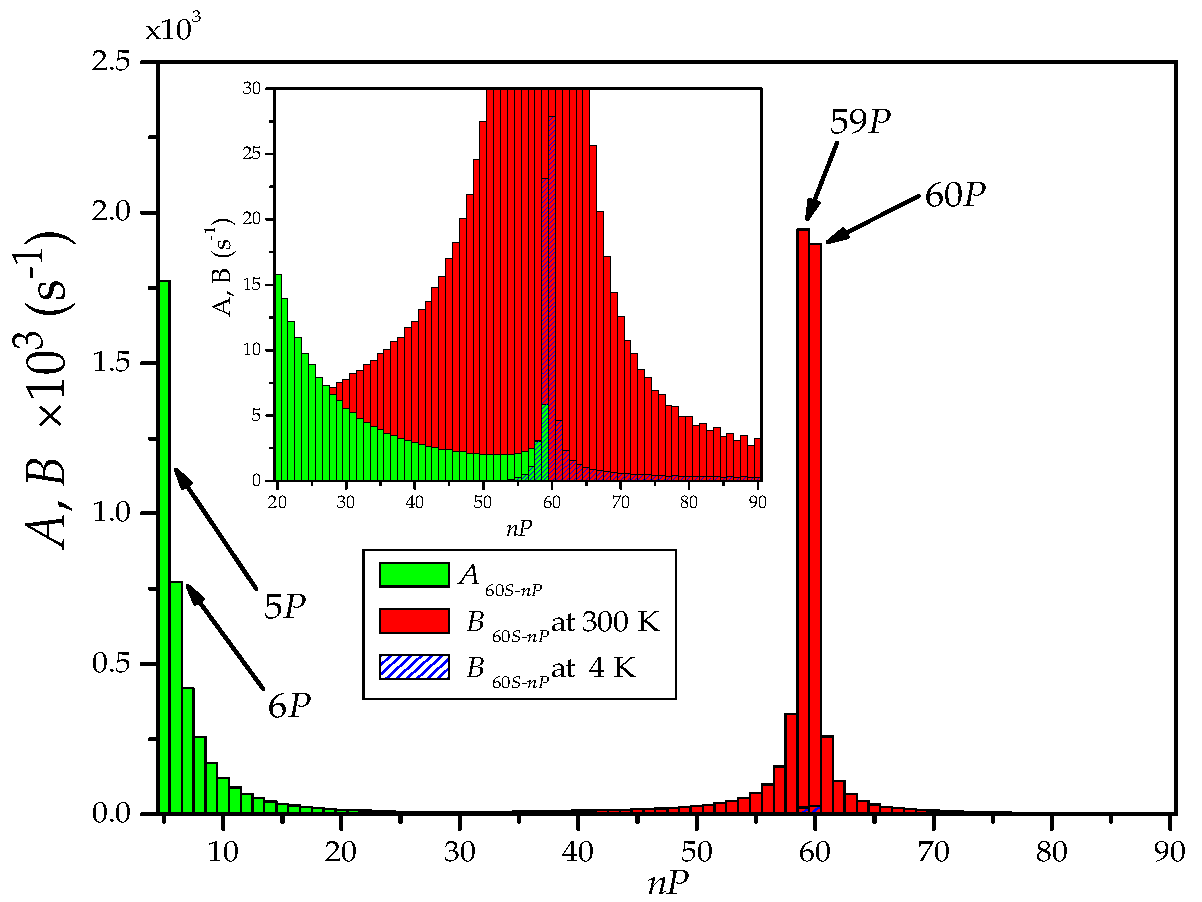
\includegraphics[width=0.7\linewidth]{figures/theory/lifetime}
	\caption[Coefficients d'Einstein de 60S vers $n\mathrm{P}_j,j\in{1/2,3/2}$]{
	Coefficients d'Einstein pour l'émission spontanée (A) et pour l'absorption et émission stimulée par le rayonnement du corps noir(B), depuis le niveau 60S vers les niveaux $n\mathrm{P}_j$.
	Pour chaque $n$, nous montrons la somme des coefficients vers $n\mathrm{P}_{j=1/2}$ et $n\mathrm{P}_{j=3/2}$.
	L'insert montre à une échelle plus adaptée la contribution du rayonnement du corps noir à $\SIv{4}{\kelvin}$.
	}
	\label{fig:matrixelements}
\end{figure}

Il est clair d'après la figure \eqref{fig:matrixelements} que le rayonnement du corps noir à $\numv{4.2}\si{\kelvin}$ contribue peu à une réduction de la durée de vie du niveau 60S par rapport à l'émission spontanée vers les niveaux de bas $n$, alors que le rayonnement du corps noir à $\numv{300}\si{\kelvin}$ aura un effet considérable, ce que confirme la table \eqref{tab:lifetime_60S}.

\begin{table}[h!]
	\centering
	\caption{Temps de vie du niveau 60S à température finie.}
	\label{tab:lifetime_60S}
	\begin{tabular}{c|c c c}
		\toprule\midrule
		\multicolumn{1}{c}{  }
		&\multicolumn{1}{c}{\text{temps de vie à }\numv{0}\si{\kelvin}}
		&\multicolumn{1}{c}{\text{temps de vie à }\numv{4.2}\si{\kelvin}}
		&\multicolumn{1}{c}{\text{temps de vie à }\numv{300}\si{\kelvin}}
		\\ 
		\midrule
		$60\mathrm{S}_{1/2}$
		&$\numv{244.5}\si{\micro\second}$
		&$\numv{239.8}\si{\micro\second}$
		&$\numv{99.4}\si{\micro\second}$\\
		\midrule
		\bottomrule
 	\end{tabular}
\end{table}

Le temps de vie du niveau 60S, de l'ordre de $\SIvv{250}{\us}$ aux températures cryogéniques, permet d'observer et manipuler celui-ci pendant des temps qui sont longs à l'échelle du mouvement d'un nuage de Rydberg.
Cependant si l'on souhaite développer une plateforme de simulation quantique, des temps d'observation beaucoup plus longs sont nécessaires.
Les atomes de Rydberg circulaires ont des durées de vie à température nulle de l'ordre de la dizaine de \si{\ms}, soit cent fois plus que le niveau 60S.
Cela fait des atomes circulaires de bons candidats pour un simulateur quantique.

\section{Les niveaux de Rydberg circulaires}\label{sec:circ_parabol}
\noindent Les niveaux de Rydberg de grand moment orbital, et en particulier les états de Rydberg circulaires, présentent une structure fine et un défaut quantique qui sont très largement négligeables.
Ils sont en cela parfaitement similaires à l'atome d'hydrogène.
On peut utiliser pour les étudier les fonctions d'onde analytiques hydrogénoïdes sans perte de précision.
Pour la même raison, le nombre quantique $j$ qui rend compte du couplage fin n'est plus nécessaire.

Les autres perturbations que peut subir le modèle de l'atome d'hydrogène, comme la présence d'un champ électrique ou magnétique extérieur en deviennent d'autant plus importantes à prendre en compte.
De plus, les niveaux circulaires étant extrêmement anisotropes, l'absence d'axe de quantification leur est préjudiciable.
Ils se mélangent alors rapidement aux niveaux voisins et il est utile de leur imposer un champ électrique, même faible, afin de pallier ce problème.
%En premier lieu, le champ extérieur définit un axe de quantification pour le moment cinétique orbital de l'atome.
%Au cours de ce paragraphe, nous considérerons qu'un axe de quantification est défini selon $(Oz)$ par un champ électrique.
%%, mais nous négligerons pour le moment l'effet Stark, par lequel la présence d'un champ électrique extérieur influence les niveaux électroniques.
%La présence d'un champ selon l'axe privilégié $(Oz)$ brise la symétrie sphérique du problème et la description des fonctions d'onde en coordonnées sphériques, donc sur la base des harmoniques sphériques, n'est plus la mieux adaptée à la situation.

\subsection{La base des états paraboliques}
\noindent	La construction de la base des harmoniques sphériques était fondée sur la conservation du moment cinétique lors du mouvement et sur l'ensemble complet d'opérateurs qui commutent (\og ECOC \fg{}) $\{\hat{H} , \hat{L}^2 , \hat{L}_z \}$
\footnote{
On a ici oublié la structure fine, qui exige lorsqu'elle est prise en compte, de remplacer $\hat{\vec{L}}$ par $\hat{\vec{J}}= \hat{\vec{L}}+\hat{\vec{S}}$.
}.%, où $\hat{J}=\hat{L}+\hat{S}$ est le moment cinétique total de l'électron.
En présence d'un champ électrique extérieur définissant l'axe $(Oz)$, le terme de couplage Stark $-\hat{\vec{d}}\cdot\vec{F} = q\hat{z}|\vec{F}|$ (cf équation \ref{eq:hamilt_Stark}) brise la symétrie sphérique du problème, de façon telle que l'opérateur $\hat{L}^2$ ne commute plus avec le hamiltonien du système.
%Rien ne contrarie cet invariant ici, mais il peut être utile d'en dégager un deuxième.
Il est alors nécessaire de trouver un nouvel invariant du mouvement, qui permettra de définir un nouvel ECOC.
Celui-ci pourra toujours contenir $\hat{L_z}$, qui reste un bon opérateur.

Dès lors que la fonction d'onde électronique reste loin du c\oe ur atomique, l'interaction entre l'électron de valence et le c\oe ur se réduit à un mouvement à force centrale.
La mécanique céleste a traité extensivement des mouvements à force centrale, et nous apprend qu'ils ont en commun l'invariance du vecteur de Runge-Lenz, qui caractérise l'excentricité des trajectoires des corps.
%
L'analogie entre l'interaction gravitationnelle des corps célestes et l'interaction coulombienne au sein des atomes permet de définir l'opérateur vectoriel :
\begin{equation}\label{eq:RungeLenz}
\hat{\vec{A}} = \frac{1}{\sqrt{-2m_e E}} \left( \frac{1}{2} (\hat{\vec{p}}\wedge\hat{\vec{L}} - \hat{\vec{L}}\wedge\hat{\vec{p}}) - m_e e^2 \frac{\vec{r}}{r} \right).
\end{equation}
Cet invariant commute avec le hamiltonien de l'atome d'hydrogène et est de même dimension que l'opérateur de moment orbital $\vec{\hat{L}}$.
Les vecteurs propres de $\hat{\vec{A}}$ prennent donc une forme similaire à ceux de $\hat{\vec{L}}$ et ses valeurs propres varient de $0$ à $\hbar(n-1)$.
%Les relations de commutation des opérateurs $\hat{L}_i$ et $\hat{a}_j$ permettent de construire un opérateur vectoriel $\{\hat{a}_x,\hat{a}_y,\hat{L}_z\}$ vérifiant les relations de commutation d'un moment cinétique :
%\begin{equation} \label{eq:commut_Leta}
%\left\{
%\begin{aligned}
%&[\hat{a}_x,\hat{a}_y]=i\hat{L}_z \\
%&[\hat{a}_y,\hat{L}_z]=i\hat{a}_x \\
%&[\hat{L}_z,\hat{a}_x]=i\hat{a}_y .\\
%\end{aligned}
%\right.
%\end{equation}
%Ce vecteur est donc un générateur des rotations dans l'espace à trois dimensions, défini par les coordonnées $\{ \text{excentricité selon }(Ox), \text{ excentricité selon }(Oy), \text{moment cinétique selon }(Oz)\}$.

Malheureusement, les opérateurs $\hat{\vec{L}}$ et $\hat{\vec{A}}$ ne commutent pas.
Il est donc nécessaire, afin d'obtenir une bonne base de description, de construire de nouveaux opérateurs qui commutent entre eux et vérifient les relations de commutation d'un moment cinétique à trois dimensions.
Les opérateurs
\begin{equation}\label{eq:defJ1J2}
\begin{aligned}
&\hat{\vec{J}}_1 = \frac{1}{2}\left( \hat{L} - \hat{A} \right)\\
\text{et} & \\
&\hat{\vec{J}}_2 = \frac{1}{2}\left( \hat{L} + \hat{A} \right).
\end{aligned}
\end{equation}
vérifient ces propriétés, et commutent avec le hamiltonien.
Au sein d'une même multiplicité, ces opérateurs vérifient 
\begin{equation}\label{eq:defJ1J2sq}
\hat{\vec{J}}_1^2 = \hat{\vec{J}}_2^2 = -\frac{\hbar^2}{4}-\frac{m_ee^4}{8E_n},
\end{equation}
ce qui s'écrit aussi
\begin{equation}\label{eq:E_j1_j2}
E=-\frac{m_ee^4}{2\hbar^2(2j_1+1)^2}=-\frac{m_ee^4}{2\hbar^2(2j_2+1)^2}~.
\end{equation}
L'on retrouve ici le fait que pour une énergie $E$ fixée et donc au sein d'une multiplicité de nombre quantique principal $n$, $\hat{\vec{J}}_1$ et $\hat{\vec{J}}_2$ définissent chacun un moment cinétique $j_{1,2}=(n-1)/2$.

Les états propres au sein d'une même multiplicité sont alors obtenus en diagonalisant $\hat{\vec{J}}_1^2$, $\hat{\vec{J}}_2^2$ et les composantes $\hat{J}_{1z}$ et $\hat{J}_{2z}$.
En notant $\hbar m_{1,2}$ les valeurs propres de $\hat{J}_{1,2~z}$, on pourra caractériser les états propres par les nombres $\{j_1,m_1,j_2,m_2\}$.
Or pour $n$ fixé, $j_1=j_2=(n-1)/2$. Ainsi, un état propre sera entièrement défini par les nombres quantiques $\ket{n,m_1,m_2}$, avec $m_1$ et $m_2$ variant entre $-(n-1)/2$ et $+(n-1)/2$.
Par construction de $\hat{\vec{J}}_{1,2}$, il est aisé de retrouver le nombre quantique magnétique $m=m_1+m_2$.
La figure \eqref{fig:parab_m1m2} propose une représentation schématique des niveaux $\ket{m_1,m_2}$ d'une même multiplicité $n$.

\begin{figure}[!h]
\centering
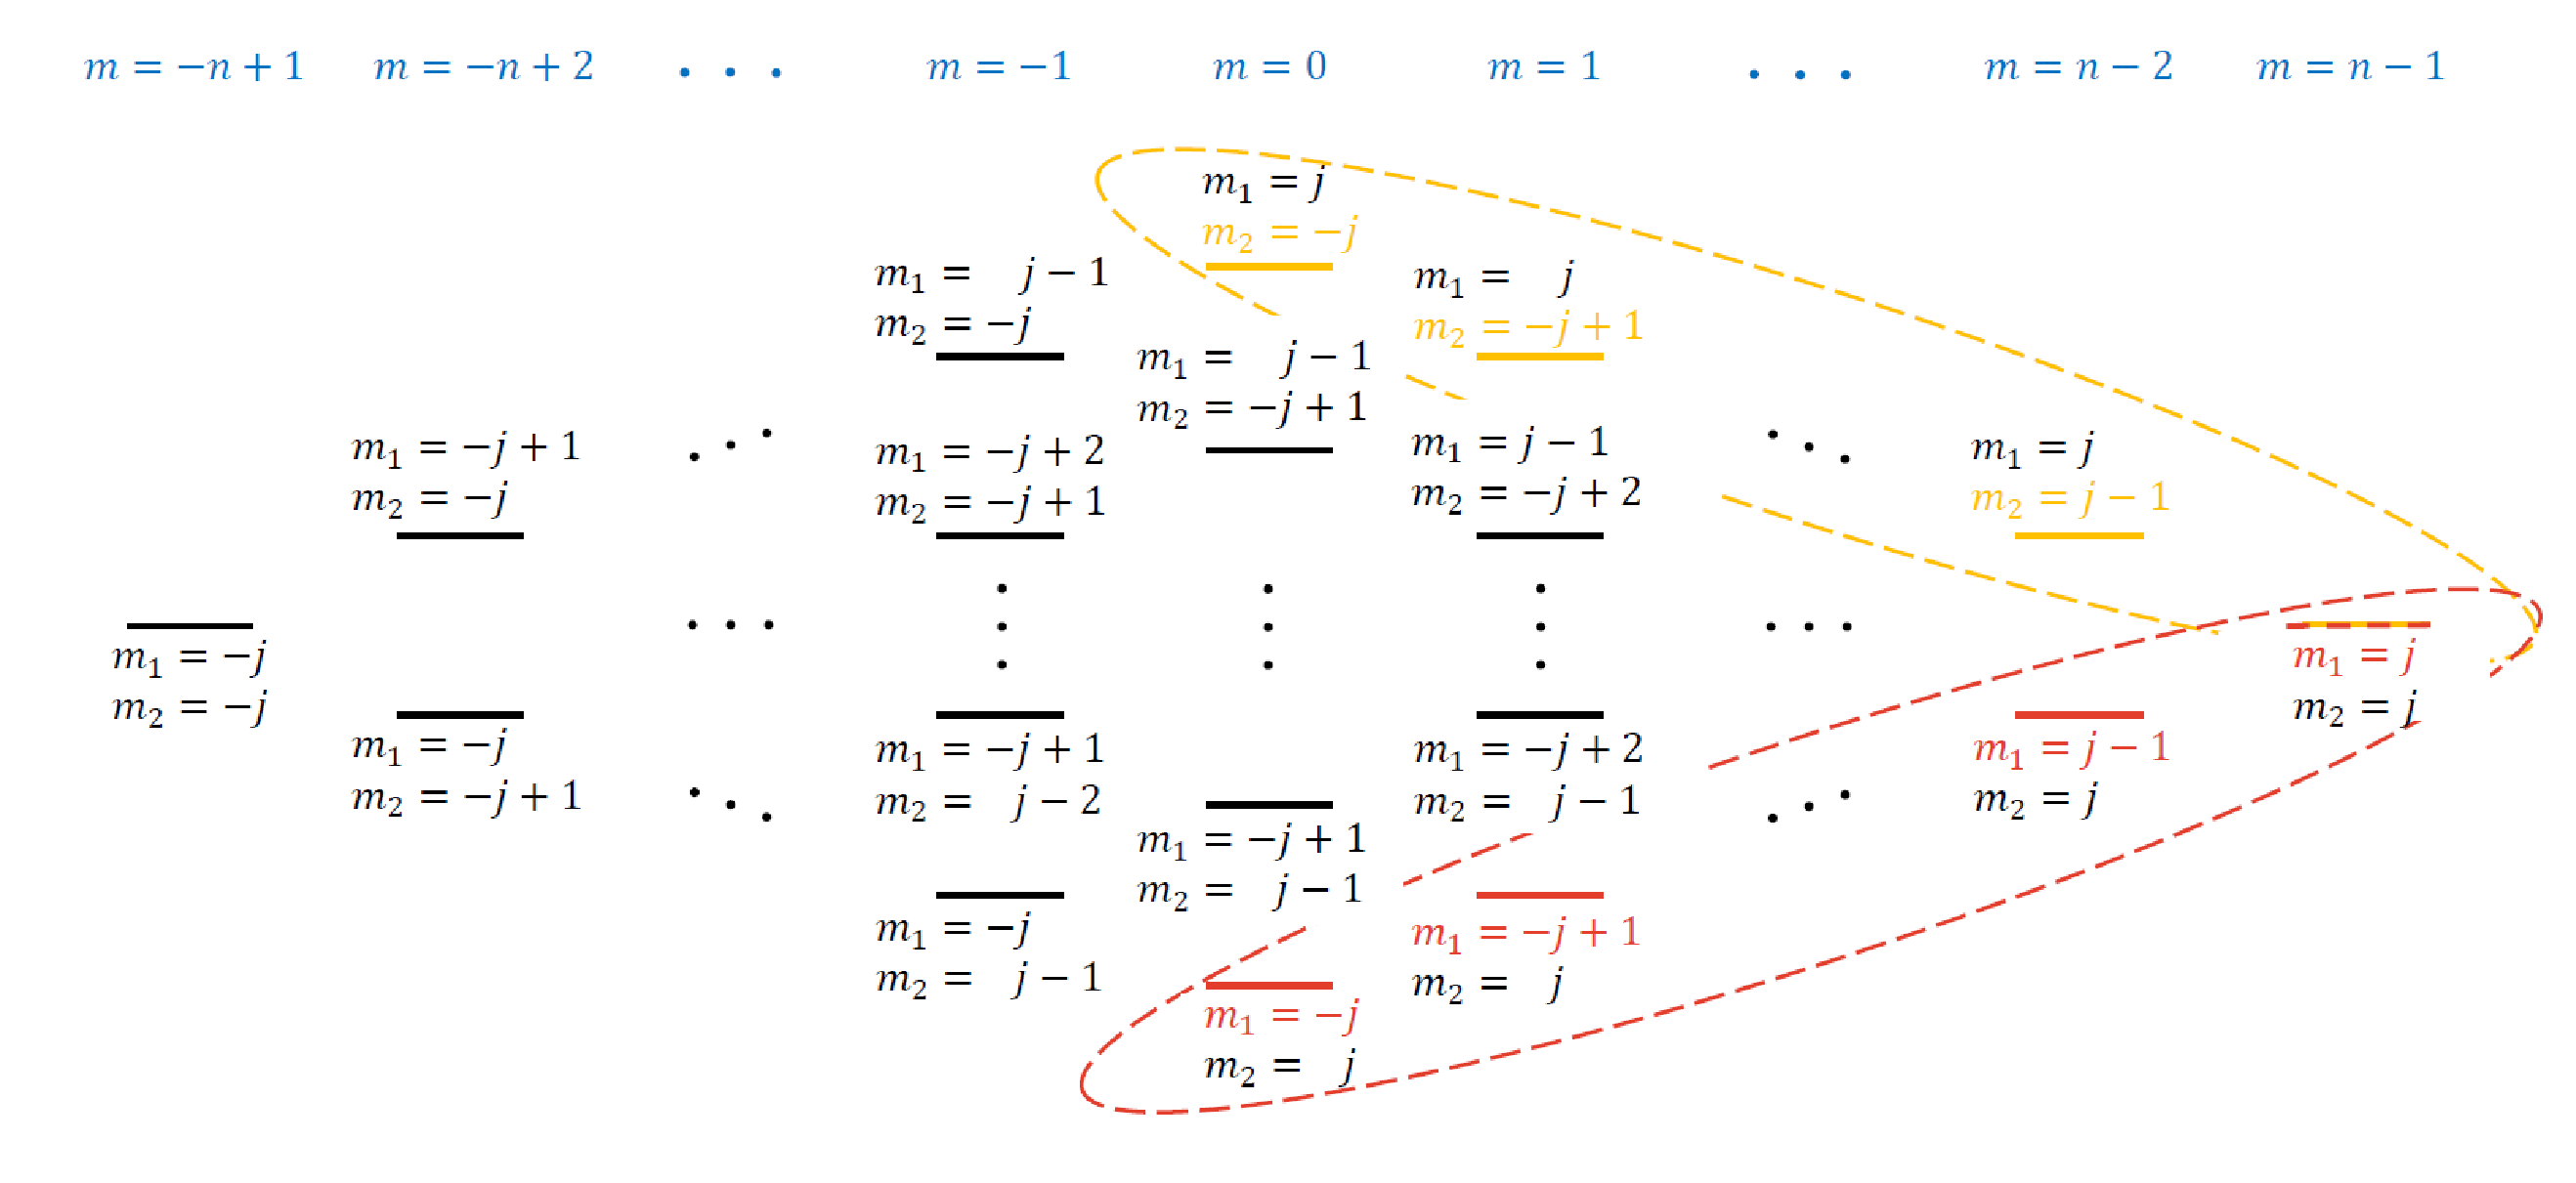
\includegraphics[width=1.\linewidth]{figures/theory/echelle_parabolique_m1m2}
\caption[Échelle des niveaux paraboliques $\ket{n,m_1,m_2}$]{
Niveaux paraboliques $\ket{n,m_1,m_2}$ de même nombre quantique principal $n$, classés horizontalement en fonction de leur nombre quantique magnétique $m=m_1+m_2$. Le nombre $j=j_1=j_2$ est la valeur des moments cinétiques $\hat{\vec{J}}_1$ et $\hat{\vec{J}}_2$ et vaut $j=(n-1)/2$.
La diagonale jaune représente la direction de variation de $m_2$ à $m_1$ fixé et la diagonale rouge la direction de variation de $m_1$ à $m_2$ fixé.
}
\label{fig:parab_m1m2}
\end{figure}


%L'équation de Schrödinger peut s'écrire dans les coordonnées paraboliques $(\xi ,\eta ,\phi )$ obtenues à partir des coordonnées sphériques $(r,\theta ,\phi)$ par la transformation :
%\begin{equation}\label{eq:coordParab}
%\hfill \xi = r(1+\cos\theta) \hfill \eta = r(1-\cos\theta)\hfill
%\end{equation}
%Dans ce système de coordonnées, l'équation de Schrödinger est séparable à condition d'introduire les nombres quantiques $n_1$ et $n2$.
%La base des états paraboliques s'obtient en introduisant les nombres quantiques paraboliques $n_1$ et $n_2$ qui sont fonction de $m_1$ et $m_2$.
%Nous préférerons ici une autre approche pour la plus grande simplicité avec laquelle elle permet de représenter les états atomiques.
%Introduisons à cet effet

Afin d'aider à la représentation des états atomiques, introduisons un nouveau nombre quantique $k=m_1-m_2$, qui quantifie l'excentricité de l'orbite électronique et permet de transformer la base $\ket{n,m_1,m_2}$ en la base $\ket{n,m,k}$ :
\begin{equation}\label{eq:base_nmk}
\left\{
\begin{aligned}
&n \text{ \begin{small}
le nombre quantique principal
\end{small}}\\
&m \text{ \begin{small}
le nombre quantique magnétique variant de
\end{small} }
-(n-1)~~ \text{ \begin{small} à \end{small}} ~~(n-1)\\
&k=m_1-m_2 \text{ \begin{small} variant de\end{small} } (-m-(n-1))~~ \text{ \begin{small} à \end{small} } ~~(-m+n-1).
\end{aligned} \right.
\end{equation}
%


\begin{figure}[!h]
\centering
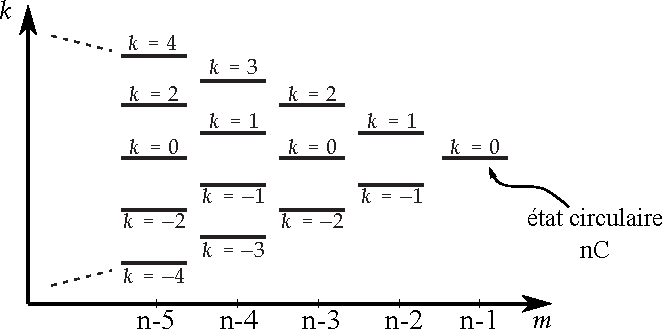
\includegraphics[width=.7\linewidth]{figures/theory/echelle_parabolique_mk}
\caption[Échelle des niveaux paraboliques $\ket{n,m,k}$]{
Niveaux paraboliques $\ket{n,m,k}$ de même nombre quantique principal $n$, classés horizontalement en fonction de leur nombre quantique magnétique $m$ et étiqueté selon le nombre quantique $k$.
Seuls les niveaux de très grand $m$ sont représentés.
}
\label{fig:parab_mk}
\end{figure}

\noindent La figure \eqref{fig:parab_mk} propose une représentation schématique des niveaux $\ket{m,k}$ de $m$ très élevé au sein d'une multiplicité $n$.

Le niveau de $m$ maximal dans une multiplicité donnée, $\ket{n,m=n-1,k=0} =\ket{n,l=n-1,m=l}$, est appelé le niveau circulaire nC.
Sa fonction d'onde électronique se réduit à un tore éloigné du c\oe ur atomique, de rayon $\sim n(n-1)a_0$, et contenu dans le plan perpendiculaire à l'axe de quantification.
La figure \eqref{fig:wavefunc50C} montre la probabilité de présence $r^2|R(r)|^2$ de l'électron dans le plan perpendiculaire à l'axe de quantification, pour le niveau de Rydberg nC. Celle-ci a une présente un rayon moyen valant
\begin{equation}\label{eq:rayon_nC}
\braket{r_{\ket{\mathrm{nC}}}}\simeq  a_0 \cdot n^2.
\end{equation}
Les niveaux de $m$ élevé mais non maximal seront appelés niveaux elliptiques en raison de la forme de leurs fonctions d'onde et seront étiquetés sur la base $\ket{n,m,k}$.
\begin{figure}[!h]
	\centering
	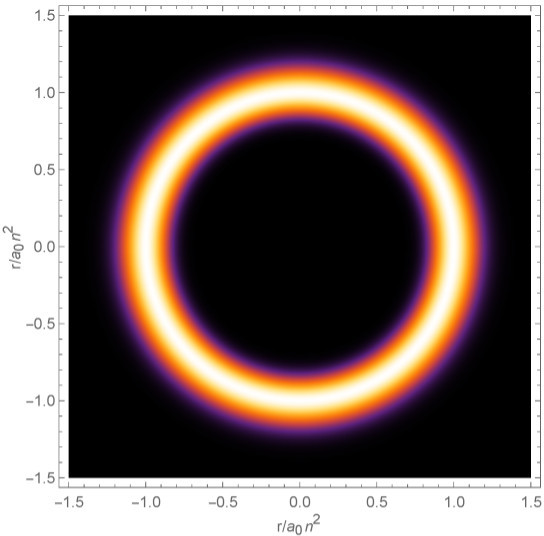
\includegraphics[width=0.5\linewidth]{figures/theory/WaveFunc_50C_}
	\caption[Fonction d'onde du niveau nC]{Probabilité de présence de l'électron dans le niveau nC : $r^2\times |R_{n\mathrm{C}}(r)|^2$, dans le plan perpendiculaire à l'axe de quantification et passant par le noyau.
	Celle-ci décrit un tore de rayon $n^2a_0$ autour du c\oe ur atomique.}
	\label{fig:wavefunc50C}
\end{figure}

%Les circulaires ont besoin d'un champ électrique pour se stabiliser.
\subsubsection*{L'effet Stark pour les atomes de grand moment cinétique}
\noindent Comme nous l'avons dit en \ref{sec:Stark}, dans la base parabolique construite autour de l'axe $(Oz)$ défini par la direction du champ électrique, le terme de couplage Stark prend une forme simple donnée par l'équation \eqref{eq:dipole_Stark} :
\begin{equation}
\label{eq:dipole_Stark2}
\hat{H}_S = q\hat{z}|\vec{F}| = q\hat{r} \sqrt{\frac{4\pi}{3}} Y_1^0  |\vec{F}|.
\end{equation}
%
Dans le cas des niveaux de Rydberg à grand moment cinétique, l'absence de défaut quantique permet de résoudre ce hamiltonien analytiquement par un traitement perturbatif de la forme \cite{TXT_BETHE_ONELECTRONATOMS} 
\begin{equation}
\label{eq:perturbative_energy}
E = E^{(0)}+E^{(1)}+E^{(2)}+\dots,
\end{equation}
où
\begin{equation}
\label{eq:Stark_circular}
\begin{aligned}
&E^{(0)} = -\frac{1}{2n^2} \\
&E^{(1)} = \frac{3}{2}nk|\vec{F}| \\
&E^{(2)} = -\frac{1}{16}\cdot (19+17n^2-9m^2-3k^2) \cdot n^4|\vec{F}|^2.
\end{aligned}
\end{equation}
%
On remarque ici que les états à $k=0$, et en particulier l'état circulaire, ne subissent l'effet Stark qu'au second ordre.

Nous pouvons désormais représenter les niveaux paraboliques $\ket{n,m,k}$ en présence d'un champ électrique qui lève leur dégénérescence.
La figure \ref{fig:parab_mk} se transforme alors en la figure \ref{fig:Stark_nmk}.
%
\begin{figure}[!h]
\centering
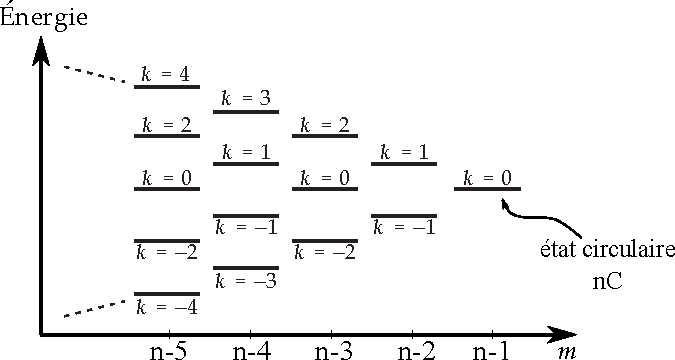
\includegraphics[width=.8\linewidth]{figures/theory/Stark_nmk}
\caption[Échelle des niveaux paraboliques $\ket{n,m,k}$]{
Énergie des niveaux paraboliques $\ket{n,m,k}$ de même nombre quantique principal $n$ en présence d'un champ électrique.
Les niveaux sont classés horizontalement en fonction de leur nombre quantique magnétique $m$ et étiqueté selon le nombre quantique $k$.
Seuls les niveaux de très grand $m$ sont représentés.
}
\label{fig:Stark_nmk}
\end{figure}
%
%Ce diagramme Stark ne ressemble pas à celui des multiplicités $n=57$ et $n=58$ de la figure \eqref{fig:Stark_60S}.
%En effet, ces multiplicités étaient définies non seulement pas leur nombre quantique principal $n$, mais aussi par leur nombre quantique magnétique $m_j = 1/2$.
%Ici au contraire, seul $n$ est fixé.

\subsection{Le niveau de Rydberg 50C : $\mathbf{\ket{n=50,l=49,m_l=49}}$}

\noindent Parmi les niveaux de Rydberg circulaires, le niveau 50C sera d'un intérêt particulier pour nous.
Ce niveau circulaire $n=50$ a une taille valant $\braket{r}_{50C} \simeq 50^2 a_0 = 2500 a_0 = \numv{132}\si{\nano\meter}$.
	

En ce qui concerne leur temps de vie, les niveaux de Rydberg circulaires ont une différence essentielle avec les niveaux de faible $l$ : les niveaux circulaires n'ont de transition dipolaire possible que vers des niveaux eux aussi à très grand $l$, et donc à très grand $n$.
Il n'y a d'ailleurs qu'une seule transition spontanée possible depuis le niveau circulaire $\text{nC}=\ket{n,l=n-1,m_l=l}$, c'est celle vers le niveau circulaire $\text{(n-1)C}=\ket{n'=n-1,l'=n'-1,m_l'=l'}$.
En effet, il n'existe aucun niveau de plus basse énergie que $\mathrm{nC}$ mais qui aurait un $l$ qui lui soit égal ou supérieur.
La figure \eqref{fig:spontem_50C49C} représente les schémas de niveaux près de l'état circulaire $n=50$ et met en évidence l'absence de toute autre transition par émission spontanée depuis le niveau 50C.
Le niveau 50C ne peut donc se désexciter spontanément que vers le niveau 49C, ce qui réduit considérablement la contribution de l'émission spontanée à son taux de désexcitation radiative.
Le calcul du dipôle de transition $\braket{50\text{C}|\hat{\vec{d}}|49\text{C}}$ donne une valeur de $\numv{1704.71} e a_0$.
En appliquant l'équation \eqref{eq:EinsteinAif} à la fréquence de transition $\mathrm{50C}\rightarrow \mathrm{49C}$ de $\SIv{54.25955}{\giga\hertz}$, on obtient un taux de désexcitation valant $\Gamma_{50C}(\SIvv{0}{\kelvin}) = A_{i=50C-f=49C} = \SIv{34.9056}{\hertz}$.
Le temps de vie à température nulle du niveau 50C est donc de $\tau_{0,50C} = \SIv{28.65}{\ms}$, soit cent fois plus que pour le niveau 60S.
\begin{figure}[!h]
	\centering
	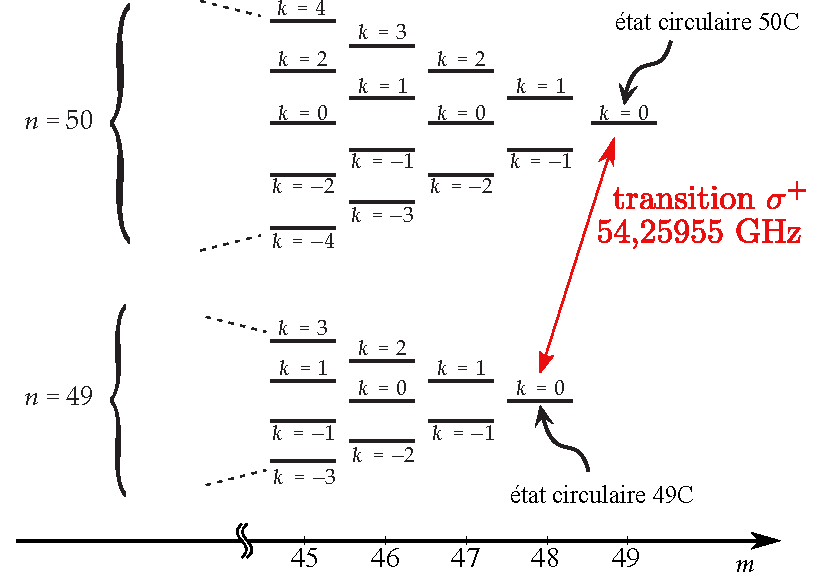
\includegraphics[width=.8\linewidth]{figures/theory/spontem_50C49C}
	\caption[Schéma de niveaux 50C-49C]{Schéma de niveaux des multiplicités $n=50$ et $n=49$ près des niveaux 50C et 49C, en présence d'un champ électrique. La seule transition possible par émission spontanée depuis le 50C est la transition vers le 49C.}
	\label{fig:spontem_50C49C}
\end{figure}

%La limitation de la durée de vie du niveau 50C provient donc en premier lieu de l'absorption et de l'émission stimulée par le rayonnement du corps noir vers les niveaux accessibles par transition dipolaire électrique.
Étant donné le faible taux de désexcitation spontanée du niveau 50C, l'effet du rayonnement du corps noir sur sa durée de vie sera important dès les très basses températures.
Le rayonnement du corps noir amplifiera non seulement le taux de désexcitation vers le niveau 49C, mais autorisera également par absorption les transitions vers les niveaux de $n$ supérieur.
Ainsi, alors que la réduction du temps de vie du niveau 60S entre $\numv{0}\si{\kelvin}$ et $\numv{4.2}\si{\kelvin}$ est faible (voir table \ref{tab:lifetime_60S}, la durée de vie du 60S est réduite de $(1-\numvv{239.8}/\numvv{244.5}) = 2\%$), la réduction du temps de vie du niveau 50C entre $\SIvv{0}{\K}$ et $\SIvv{4.2}{\K}$ est bien plus importante et se porte à $(1-\numv{8.36}/\numv{28.65}) = 71\%$.
\`A température ambiante de $\numv{300}\si{\kelvin}$, la durée de vie de 50C est même réduite à $\numv{122}\si{\micro\second}$, très similaire à celle du niveau 60S.
La figure \eqref{fig:lifetime_50C} montre l'évolution de la durée de vie du niveau 50C en fonction de la température de rayonnement du corps noir, calculée à partir des équations \eqref{eq:EinsteinBif} et \eqref{eq:BoseStat}.


\begin{figure}[!h]
	\centering
	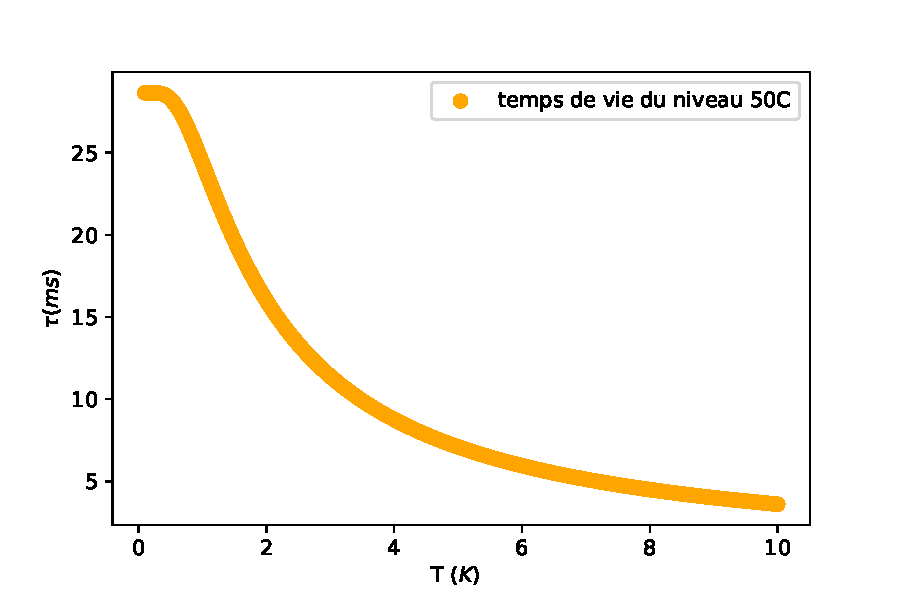
\includegraphics[width=0.8\linewidth]{figures/theory/lifetime_50C}
	\caption[Durée de vie du niveau 50C]{Durée de vie radiative du niveau de Rydberg 50C en fonction de la température de rayonnement du corps noir.}
	\label{fig:lifetime_50C}
\end{figure}

\newpage
Nous avons désormais une bonne connaissance des caractéristiques des atomes de Rydberg individuels, en particulier dans les niveaux 60S et 50C.
Ce sont de très grands atomes, avec de très grands moments dipolaires de transition, et un temps de vie très long.
Comment se comportent ces atomes de Rydberg lorsqu'ils ne sont plus isolés mais proches les uns des autres ?

%\section{Atomes de Rydberg en interaction}
%	\subsection{Deux atomes de Rydberg}
%		\noindent hamiltonien d'interaction entre deux dipôles
%		\[
%		V_{dd} = \frac{1}{4\pi\epsilon_0 r^3} \left( \mathbf{d_1}\cdot \mathbf{d_2} - 3(\mathbf{d_1}\cdot \frac{\mathbf{r}}{r})(\mathbf{d_2}\cdot\frac{\mathbf{r}}{r}) \right)
%		\]
%		\noindent de l'interaction dipole-dipole générale au terme de Van der Waals en $1/r^6$ \\
%		\noindent terme d'énergie et terme d'échange
%	\subsection{les interactions entre Rydberg de bas $l$}
%		\noindent origine du $C_6$ pour 60s-60s et $C_6/A_6$ avec les voisins\\
%		reprendre Raul.figI.3 qui présente la partie radiale du dipôle 60s-ns en fonction de n\\
%		\noindent principe du blocage dipolaire et facilitation (rapide)
%	\subsection{les interactions entre Rydberg circulaires}
%		\noindent $C_6$ pour 50c-50c et $C_6/A_6$ avec les voisins \\
%		\noindent attention à l'anisotropie\\
%		équivalent de la figure ci dessus (Raul.figI.3) pour les 50c, à modifier pour l'anisotropie

%\section{Atomes de Rydberg en interaction}
Dans cette thèse, nous allons nous intéresser aux interactions entre plusieurs atomes de Rydberg voisins, dans des niveaux identiques ou proches en énergie.
Le reste de ce chapitre est consacré au calcul de ces interactions et à leur application aux deux cas qui nous concernent : autour des niveaux 60S et 50C.

	\subsection{Deux atomes de Rydberg qui se parlent}
L'opérateur de moment dipolaire entre deux niveaux de Rydberg proches est grand, comme nous l'avons évoqué.
En cela, les atomes de Rydberg sont de très bonnes antennes pour le rayonnement électromagnétique lorsque celui-ci est résonant avec les fréquences de transition entre niveaux proches.
Cette caractéristique s'accentue fortement lorsque le nombre quantique principal augmente, car le moment dipolaire varie en $n^{*2}$.
Ces grands moments de transition dipolaires font aussi apparaître une interaction importante entre deux atomes de Rydberg différents : bien qu'ils restent des objets neutres électriquement, ces grands dipôles se voient très bien de loin.
En électromagnétisme classique, le terme de couplage entre deux dipôles électriques s'écrit \cite{TXT_JACKSON}
\begin{equation}\label{eq:classicDipole}
V_{dd}(\vec{r}) = \frac{1}{4\pi\epsilon_0 r^3} \left( \vec{d_1}\cdot \vec{d_2} - 3(\vec{d_1}\cdot \frac{\vec{r}}{r})(\vec{d_2}\cdot\frac{\vec{r}}{r}) \right)
\end{equation}
où $\vec{d_1}$ décrit le premier dipôle, $\vec{d_2}$ le deuxième dipôle et $\vec{r}$ le vecteur d'espace qui les sépare.
On peut alors écrire, par analogie, le hamiltonien d'interaction entre deux atomes en remplaçant les dipôles classiques par les opérateurs dipôle électrique de chaque atome.
La distance entre les atomes sera cependant traitée de façon classique, en supposant que la distance entre les atomes est très grande devant l'extension spatiale de leurs fonctions d'onde.
% C'est ce qu'on appelle l'approximation dipolaire. FAUX (commentaire Michel 15 sept
Le potentiel d'interaction dipolaire s'écrit dans ce cas
\begin{equation}\label{eq:quantDipole}
\begin{aligned}
\hat{V}_{dd}(\vec{r}) &= \frac{1}{4\pi\epsilon_0 r^3} \left( \vec{\hat{d}_1}\cdot \vec{\hat{d}_2} - 3(\vec{\hat{d}_1}\cdot \frac{\vec{r}}{r})(\vec{\hat{d}_2}\cdot\frac{\vec{r}}{r}) \right) \\
&= \frac{q^2}{4\pi\epsilon_0 r^3} \left( \vec{\hat{r}_1}\cdot \vec{\hat{r}_2} - 3(\vec{\hat{r}_1}\cdot \frac{\vec{r}}{r})(\vec{\hat{r}_2}\cdot\frac{\vec{r}}{r}) \right).
\end{aligned}
\end{equation}
%
Remarquons que ce terme dépend du produit des opérateurs de transition dipolaire électrique de chaque atome. L'interaction entre atomes de Rydberg varie donc comme $(n^{*2})^2 = n^{*4}$.

\bigskip
Calculer l'interaction entre deux atomes de Rydberg revient à diagonaliser le hamiltonien total du système des deux atomes dans l'espace de Hilbert des états possibles pour la paire d'atomes.
Sans autre \textit{a priori}, une base naturelle pour cet espace est le produit tensoriel $\ket{R_1}\otimes\ket{R_2}$ des états de chaque atome.
Dans cette base, le hamiltonien du système s'écrit
\begin{equation}\label{eq:hamilt2atoms}
\hat{H} = \hat{H}_{0,1} + \hat{H}_{0,2} + \hat{V}_{dd}(\vec{r})
\end{equation}
où $\hat{H}_{0,i}$ est le hamiltonien de l'atome $i$ isolé.

En l'absence de champ électrique ou magnétique extérieur, l'axe de quantification pour les niveaux de chaque atome n'est pas déterminé.
Il semble naturel de choisir alors comme axe de quantification le vecteur qui sépare les atomes.
Dans cette géométrie, le potentiel d'interaction dipolaire prend la forme
\begin{equation}\label{eq:Vdd_rr1r2}
\begin{aligned}
\hat{V}_{dd}(\vec{r})=&
-\frac{q^2}{4\pi\epsilon_0}\frac{\hat{r}_1\hat{r}_2}{r^3}\frac{4\pi}{3} \times
\left( \hat{Y}^1_1(\theta_1,\phi_1) \hat{Y}^{-1}_1(\theta_2,\phi_2) \right. \\
&\left. + \hat{Y}^{-1}_1(\theta_1,\phi_1) \hat{Y}^{1}_1(\theta_2,\phi_2)
+ 2\hat{Y}^{0}_1(\theta_1,\phi_1) \hat{Y}^{0}_1(\theta_2,\phi_2)
\right)
\end{aligned}
\end{equation}
où les $Y^{m_l}_l$ sont les harmoniques sphériques, solutions des équations de Legendre \cite{TXT_COHEN1FR}.
Dans cette base, l'opérateur $\hat{V}_{dd}$ préserve le nombre quantique magnétique total $M=m_{j1}+m_{j2}$.
Cette condition définit un sous-espace des niveaux de même $M$ pour la paire d'atomes, sous-espace qui a une dimension infinie.
Il sera donc nécessaire, pour calculer l'interaction entre les deux atomes, de tronquer ce sous-espace.
Dans le sous-espace tronqué, nous pouvons diagonaliser le hamiltonien \eqref{eq:hamilt2atoms} pour chaque distance interatomique $r$.

\subsection{Deux atomes dans le même niveau de Rydberg}
Dans le cas de deux atomes dans le même niveau de Rydberg $a$, la règle de sélection $\Delta l = \pm 1$ impose que $\braket{aa|\hat{V}_{dd}|aa} = 0$.
L'opérateur d'interaction dipolaire n'agit donc sur la paire $\ket{aa}$ que comme une perturbation de second ordre, \textit{via} le couplage à des niveaux de paire intermédiaires $\ket{cd}$.
La figure \eqref{fig:Dip_aacd} représente ce couplage au second ordre.
L'énergie d'interaction résultant de cette perturbation prend la forme
\begin{equation}\label{eq:VdW_aacd}
C_{aa}(r)=\sum_{\ket{cd}}{\frac{\braket{aa|\hat{V}_{dd}|cd}\braket{cd|\hat{V}_{dd}|aa}}{2E_a - E_c - E_d}}  = \frac{C_{6,aa}}{r^6}
\end{equation}
où $E_i$ est l'énergie d'un atome de Rydberg individuel dans l'état $i$.
L'interaction dipolaire prend donc la forme d'une interaction de Van der Waals en $1/r^6$, avec un coefficient valant $C_{6,aa}$.

\begin{figure}[!h]
\centering

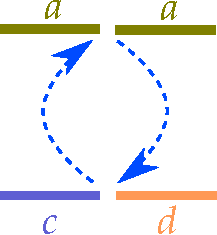
\includegraphics[width=0.3\linewidth]{figures/theory/dipole_coupling_aacd}
\caption[Couplage dipolaire entre mêmes niveaux de Rydberg]{Schéma du couplage dipolaire entre deux atomes dans des niveaux de Rydberg $a$ identiques : le couplage s'effectue au second ordre \textit{via} les niveaux $c$ et $d$.}
\label{fig:Dip_aacd}
\end{figure}

La situation se complique lorsque l'un des niveaux intermédiaires $\ket{cd}$ est quasi-dégénéré avec le niveau $\ket{aa}$, c'est-à-dire lorsque $\braket{aa|\hat{V}_{dd}|cd} \gg |2E_a-E_c-E_d|$.
Le développement perturbatif est en effet invalidé sous cette condition et il est nécessaire de traiter le problème différemment.
Si $\ket{c}=\ket{d}$, alors le sous-espace à observer est composé des deux états $\ket{aa}$ et $\ket{cc}$ et l'on a $E_c\simeq E_a$.
Le hamiltonien d'interaction s'écrit alors
\begin{equation}\label{eq:forster_aacc}
H_{aa-cc} = \bordermatrix{~ 	&\ket{aa} 	& \ket{cc} \cr
	\ket{aa}		&2E_a 		& \frac{\Braket{aa|V_{dd}|cc}}{r^3}	\cr 
	\ket{cc} 		& \frac{\Braket{aa|V_{dd}|cc}}{r^3} 		&2E_a\cr} \ .
\end{equation}
%
Les états propres de ce hamiltonien sont les combinaisons symétrique et antisymétrique $(\ket{aa}\pm\ket{cd})/\sqrt{2}$, et présentent les énergies propres
\begin{equation}\label{eq:forster_aacc_energies}
2E_a \pm \Delta E_{dd} = 2E_a \pm\frac{\braket{aa|V_{dd}|cc}}{r^3}= 2E_a \pm\frac{C_{3,aa}}{r^3}.
\end{equation}

Si, au contraire, $\ket{c}\neq \ket{d}$, on est alors en présence de trois états dégénérés : $\ket{aa}$, $\ket{cd}$ et $\ket{dc}$.
Il est utile de réécrire ceux-ci en combinant $\ket{cd}$ et $\ket{dc}$ symétriquement et anti-symétriquement en $\ket{C}=(\ket{cd}+\ket{dc})/\sqrt{2}$ et $\ket{NC}=(\ket{cd}-\ket{dc})/\sqrt{2}$.
En effet, $\hat{V}_{dd}$ ne couple pas le niveau $\ket{aa}$ avec le niveau $\ket{NC}$.
On peut donc appliquer le traitement réservé jusqu'ici au cas $\ket{c}=\ket{d}$ en remplaçant $\ket{cc}$ par $\ket{C}$.
Nous obtenons donc deux états propres $(\ket{aa}\mp \ket{C})/\sqrt{2}$ avec les énergies
\begin{equation}\label{eq:forster_aacd_energies}
2E_a \pm \Delta E_{dd} = 2E_a \pm\frac{\braket{aa|V_{dd}|C}}{r^3}= 2E_a \pm\frac{\braket{aa|V_{dd}|cd}}{r^3}= 2E_a \pm\frac{C_{3,aa}}{r^3}.
\end{equation}
Ces cas particuliers sont analogues à ce que l'on appelle dans d'autres contextes les résonances de Förster \cite{MX_BROWAEYSDD14}.

\subsection{Deux atomes dans des niveaux de Rydberg différents}
\label{subsec:interaction_diff_levels}
Intéressons-nous désormais aux interactions entre deux atomes de Rydberg dans les états $a$ et $b$.
Il y a alors deux états de paire dégénérés $\ket{ab}$ et $\ket{ba}$.
De même que précédemment, les termes de couplage $\braket{ab|\hat{V}|ab}=\braket{ba|\hat{V}|ba}$ sont nuls.
L'on peut tout de même introduire un opérateur potentiel effectif $V_{eff}$ pour le système à deux niveaux $\ket{ab}$ et $\ket{ba}$, qui tiendra compte du couplage éventuel au premier ordre entre $\ket{ab}$ et $\ket{ba}$ mais également des couplages de second ordre avec des états intermédiaires.
Les éléments de matrice de $V_{eff}$ sont
%
\begin{equation}\label{eq:Cab_Aab}
\begin{aligned}
&C_{ab}=\braket{ab|V_{eff}|ab}=\braket{ba|V_{eff}|ba} \\
\text{et} &\\
&A_{ab}=\braket{ab|V_{eff}|ba}=\braket{ab|V_{eff}|ba}.
\end{aligned}
\end{equation}
%
L'hamiltonien d'interaction s'écrit sous forme matricielle
\begin{equation}\label{eq:MatrixCab_Aab}
V_{eff} = \bordermatrix{~ 	&\ket{ab} 	& \ket{ba} \cr
	\ket{ab}		&C_{ab} 		&A_{ab}	\cr 
	\ket{ba} 		&A_{ab} 		&C_{ab} \cr} \ .
\end{equation}
%
Les termes diagonaux de ce hamiltonien représentent l'interaction directe d'un état de paire avec lui-même, qui se calcule donc comme une perturbation de second ordre \textit{via} les niveaux intermédiaires $\ket{cd}$.
Comme c'était le cas pour deux atomes dans le même état de Rydberg, cette interaction prend la forme de Van der Waals avec un coefficient $C_{6,ab}$ :
\begin{equation}\label{eq:VdW_abab}
C_{ab}(r)=\sum_{\ket{cd}}{\frac{\braket{ab|\hat{V}_{dd}|cd}\braket{cd|\hat{V}_{dd}|ab}}{E_a + E_b - E_c - E_d}}  = \frac{C_{6,ab}}{r^6}.
\end{equation}

Les termes non-diagonaux $A_{ab}$ correspondent eux à une interaction au cours de laquelle les deux atomes échangent leurs états.
Si la transition $a\rightarrow b$ est autorisée par les règles de sélection dipolaires, alors cette interaction d'échange est un couplage \textit{direct} de $\ket{ab}$ et $\ket{ba}$.
Il varie donc comme un potentiel dipolaire en $1/r^3$.
Dans le cas contraire, l'interaction d'échange sera un couplage dipolaire indirect au second ordre, variant donc en $1/r^6$, voire d'ordre supérieur, comme l'illustre la figure \eqref{fig:Dip_abab}.

\begin{figure}[!h]
\centering
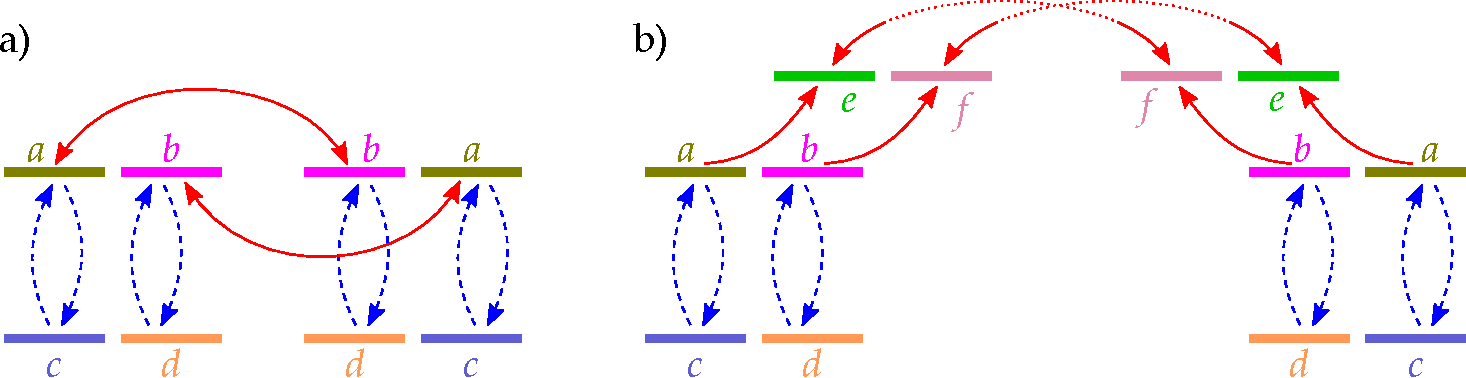
\includegraphics[width=0.9\linewidth]{figures/theory/dipole_coupling_abab}
\caption[Couplage dipolaire entre niveaux de Rydberg différents]{Schéma du couplage dipolaire entre deux atomes dans des niveaux de Rydberg différents $a$ et $b$ : le couplage $ab-ab$ s'effectue au second ordre \textit{via} les niveaux $c$ et $d$. Le couplage $ab-ba$ peut s'effectuer à l'ordre 1(\textbf{a}), à l'ordre 2 via des niveaux intermédiaires $e$ et $f$(\textbf{b}), ou plus encore.}
\label{fig:Dip_abab}
\end{figure}


Lorsque les termes d'échange $A_{ab}$ deviennent comparables aux termes d'interaction directe $C_{ab}$, il peut être judicieux de diagonaliser le hamiltonien effectif \eqref{eq:MatrixCab_Aab}.
En effet, les états propres de celui-ci, qui sont les combinaisons symétrique et anti-symérique $(\ket{ab}\pm \ket{ba})/\sqrt{2}$, ne sont plus dégénérés et présentent respectivement des déplacements d'énergie
\begin{equation}
\label{eq:shift_abab}
\Delta E_{dd} = C_{ab} \mp A_{ab}.
\end{equation}

Afin d'illustrer la discussion des interactions que nous venons de présenter, nous allons les appliquer à nos deux exemples que sont le niveau 60S et le niveau 50C.
Dans les deux cas, le calcul numérique consiste à diagonaliser le hamiltonien \eqref{eq:hamilt2atoms} à tous les ordres perturbatifs, en limitant l'espace de Hilbert à quelques centaines d'états de paire et en traitant la distance interatomique de façon classique.

\subsection{Les interactions dipolaires du niveau 60S}

\subsubsection*{L'interaction 60S-60S}
Dans le cas de l'état $\ket{60\text{S},60\text{S}}$, le terme dominant dans la somme \eqref{eq:VdW_aacd} permettant de calculer le coefficient de Van der Waals $C_{6,\text{60S60S}}$ est le coulage avec les paires $\ket{60\text{P}_j,59\text{P}_j}$.
Puisque $E_{60S}-E_{59P}>E_{60P}-E_{60S}$, le dénominateur du terme de couplage principal dans \eqref{eq:VdW_aacd} est positif.
On en déduit que l'interaction 60S-60S, et plus généralement toute interaction dipolaire nS-nS, est toujours répulsive.
%
\begin{figure}[!h]
\centering
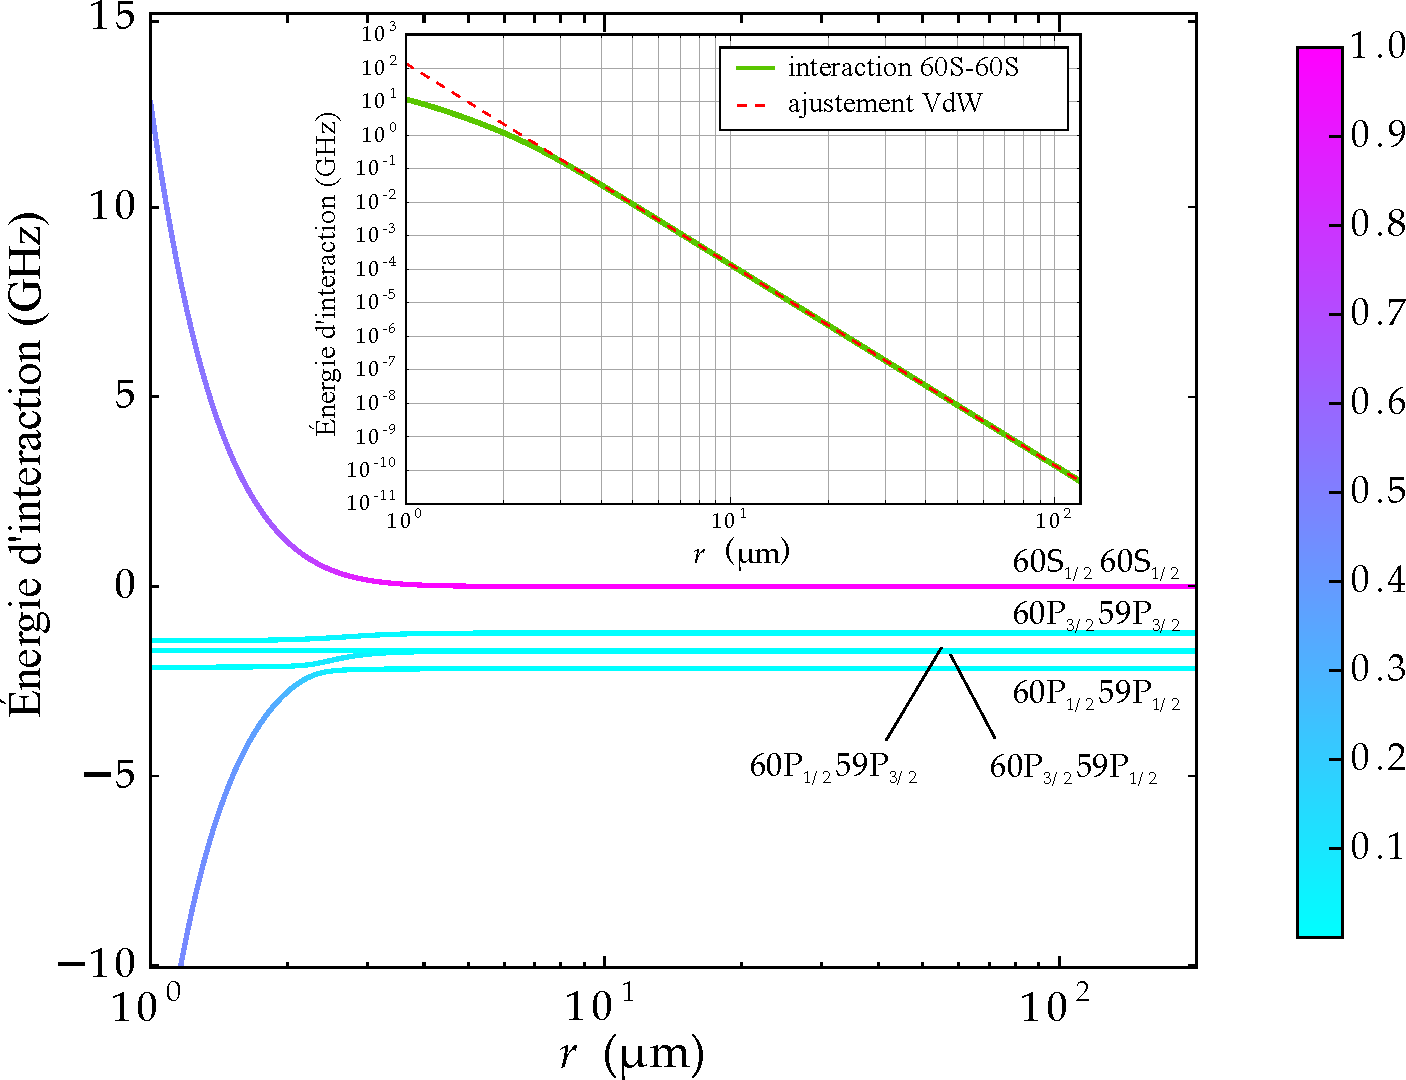
\includegraphics[width=0.8\linewidth]{figures/theory/VdW_60S60S}
\caption[Interaction dipolaire 60S-60S]{Déplacement en énergie de la paire 60S-60S par interaction de Van der Waals. Les différents sous-niveaux $\ket{60\text{P}_j,59\text{P}_j}$ sont représentés. L'échelle de couleur représente le carré de la projection sur l'état non perturbé $\ket{60\text{S},60\text{S}}$.
L'insert représente le déplacement d'énergie en échelle log-log et son ajustement sous la forme de Van der Waals.}
\label{fig:VdW_60s60s}
\end{figure}
%
Le calcul numérique de l'interaction 60S-60S et son ajustement sous la forme de Van der Waals, représentés en figure \eqref{fig:VdW_60s60s}, donnent la valeur
\begin{equation}
\label{eq:C660S}
C_{6,60S60S} = \numv{137.6(1)}\si{\giga\hertz\raiseto{6}\micro\meter}.
\end{equation}

L'ajustement de Van der Waals fonctionne très bien aux distances supérieures à $\sim\SIvv{3}{ \micro\meter}$.
Cependant, aux très courtes distances, la paire $\ket{60\text{S},60\text{S}}$ est très fortement couplée aux niveaux $\ket{60\text{P}_j,59\text{P}_j}$.
La distance critique est celle à laquelle le couplage dipolaire est aussi fort que la différence d'énergie entre les deux états de paire non perturbés, soit ici $\sim \SIv{2}{\giga\hertz}$.
En deçà de cette distance, les états propres du hamiltonien s'éloignent de plus en plus de l'état non perturbé $\ket{60\text{S},60\text{S}}$ et l'interaction évolue vers une interaction dipolaire résonante en $1/r^3$.

\subsubsection*{Les interactions 60S-$nl$}
Le niveau 60S interagit également avec des états de $n$ et $l$ différents.
Il convient alors, comme nous l'avons montré en \eqref{subsec:interaction_diff_levels}, de calculer non seulement les coefficients de Van der Waals $C_{ab}$, mais aussi les éléments de matrice d'échange $A_{ab}$.
De plus, il est possible ici d'avoir des termes d'échange dûs à un couplage dipolaire direct et qui varient donc en $r^3$.

\begin{figure}[h]
\centering
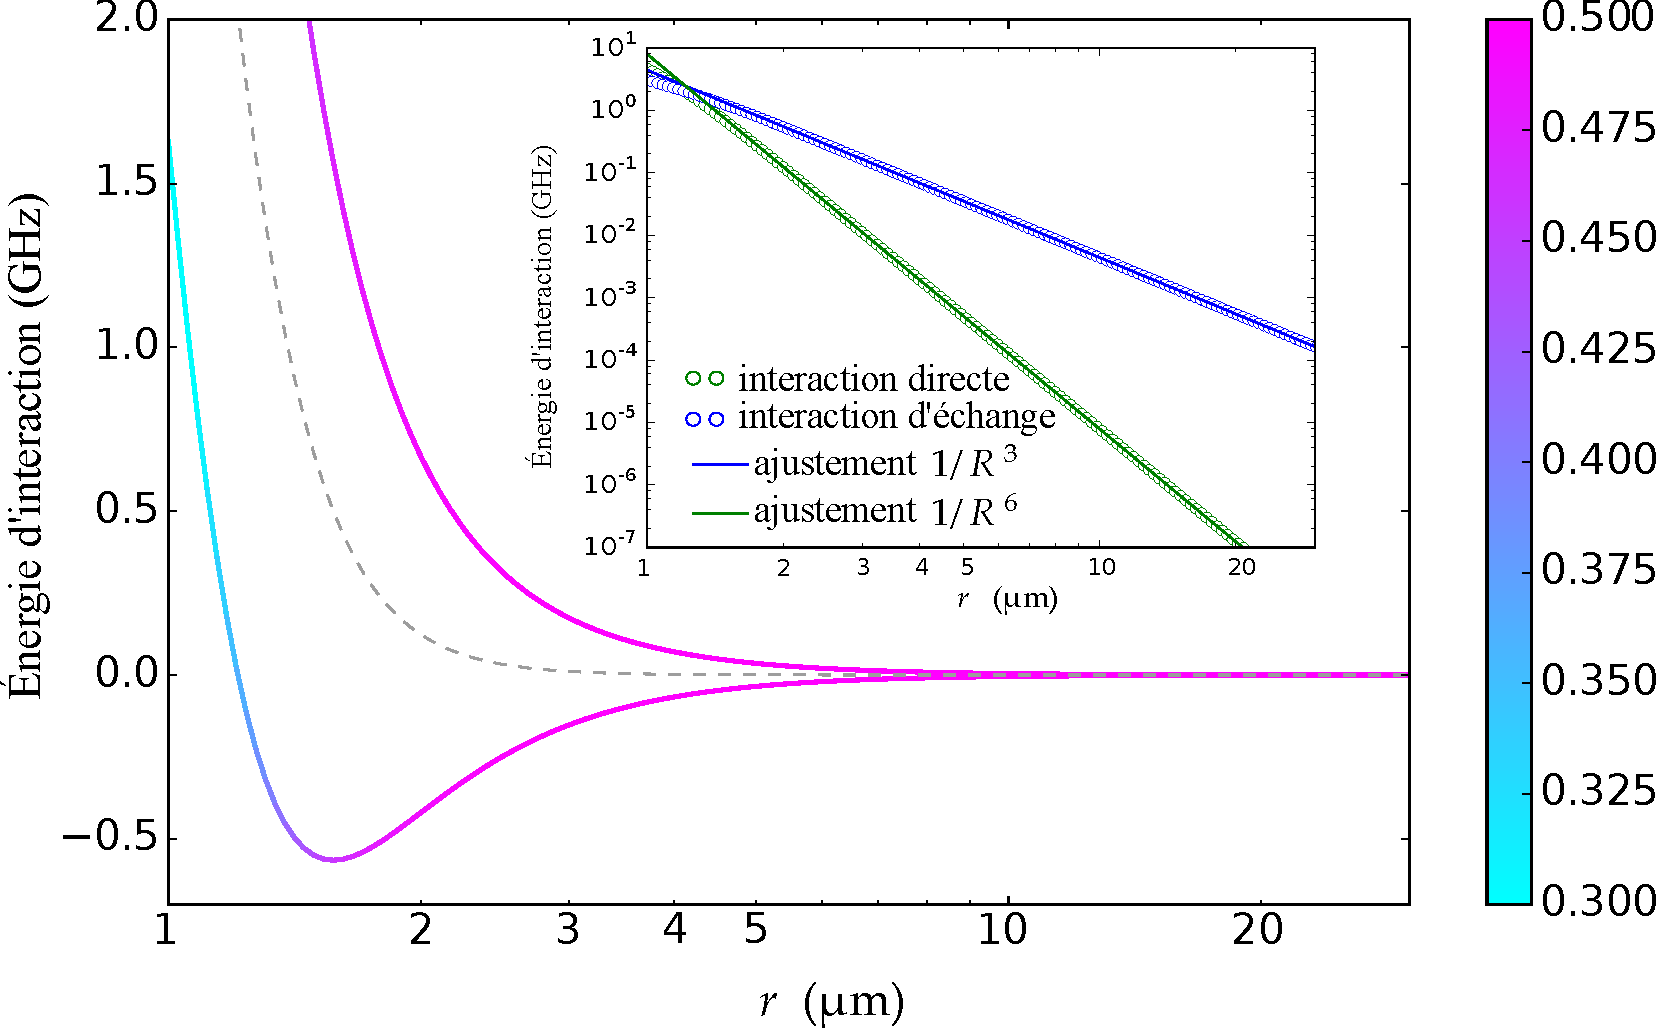
\includegraphics[width=0.8\linewidth]{figures/theory/VdW_60S60P}
\caption[Interaction dipolaire 60S-60P$_{3/2}$]{Énergie de la paire 60S-60P$_{3/2}$ en présence de l'interaction dipolaire.
Les branches inférieure et supérieure correspondent respectivement aux superpositions symétrique et antisymétrique des deux niveaux de départ.
L'échelle de couleur représente le carré de la projection sur l'état non perturbé $\ket{60\text{S},60\text{P}_{3/2}}$.
La ligne pointillée représente le déplacement en énergie dû à l'interaction directe.
L'insert représente le déplacement d'énergie ainsi que le terme d'échange en échelle log-log et leurs ajustements en $1/r^6$ et $1/r^3$ respectivement.
}
\label{fig:VdW_60S60P}
\end{figure}

La figure \eqref{fig:VdW_60S60P} montre par exemple le résultat du calcul de l'interaction dipolaire pour une paire 60S-60P$_{3/2}$.
Aux grandes distances, l'état de la paire est projeté uniformément sur les deux superpositions symétrique et anti-symétrique.
Aux plus courtes distances cependant, d'autres niveaux contaminent la paire, qui n'est plus dans une superposition de $\ket{60\text{S}}$ et $\ket{60\text{P}_{3/2}}$.

En procédant dela même façon, on peut obtenir les coefficients d'interaction dipolaire pour n'importe quelle paire 60S-$nl$. La table \eqref{tab:VdWcoef_60S_nl} synthétise les résultats des calculs numériques pour plusieurs paires contenant le niveau 60S.

\begin{table}[h!]
	\centering
	\caption[Coefficients de Van der Waals 60S-nl]{Coefficients de Van der Waals pour les interactions de paire entre le niveau 60S et différents niveaux voisins $nl$.}
	\label{tab:VdWcoef_60S_nl}
	\begin{tabular}{c c c c}
		\toprule\midrule
%		\multicolumn{1}{c}{  }
%		&\multicolumn{1}{c}{\text{temps de vie à }\numv{0}\si{\kelvin}}
%		&\multicolumn{1}{c}{\text{temps de vie à }\numv{4.2}\si{\kelvin}}
%		&\multicolumn{1}{c}{\text{temps de vie à }\numv{300}\si{\kelvin}}
%		\\ 
		{ }&$C_6$ (\si{\giga\hertz\raiseto{6}\micro\meter}) & $A_6$ (\si{\giga\hertz\raiseto{6}\micro\meter}) & $A_3$ (\si{\giga\hertz\raiseto{3}\micro\meter})
		\\
		\midrule
		$60\text{S}_{1/2}, 60\text{S}_{1/2}$
		&$\SIv{137.6}{}$
		&$\SIv{0}{}$
		&$\SIv{0}{}$\\
		$60\text{S}_{1/2}, 57\text{S}_{1/2}$
		&$\SIv{-43.265}{}$
		&$\SIv{0.325}{}$
		&$\SIv{0}{}$\\
		$60\text{S}_{1/2}, 61\text{S}_{1/2}$
		&$\SIv{290.125}{}$
		&$\SIv{246.475}{}$
		&$\SIv{0}{}$\\
		$60\text{S}_{1/2}, 60\text{P}_{3/2}$
		&$\SIv{7.976}{}$
		&$\SIv{0}{}$
		&$\SIv{4.411}{}$\\
		\midrule
		\bottomrule
 	\end{tabular}
\end{table}



\subsection{Les interactions dipolaires du niveau 50C}
	
\noindent L'interaction dipolaire entre atomes de Rydberg de très grand moment cinétique est rendue plus complexe du fait de leur forte anisotropie.
En effet, l'interaction entre deux dipôles dépend de l'orientation relative de ceux-ci.
Dans le cas des niveaux $l=0$ tel que le 60S, le problème ne se posait pas car ces niveaux sont à symétrie sphérique.
Dès lors que l'on s'intéresse à l'interaction entre des niveaux à symétrie cylindrique, il est indispensable de savoir comment les atomes s'orientent l'un par rapport à l'autre.
L'interaction dipolaire entre atomes circulaires est encore compliquée par l'introduction d'un champ électrique extérieur, qui déplace et déforme les niveaux par effet Stark.
Le détail de l'interaction dipolaire entre atomes circulaires en présence d'un champ sera discuté au chapitre \ref{chapter:circsim}, mais nous prendrons le temps ici de développer la situation la plus simple :
celle de deux atomes dans le niveau 50C dont les deux orbites sont contenues dans le même plan, comme l'illustre la figure \eqref{fig:double_torus}.
%
\begin{figure}[!h]
\centering
\vspace{1em}
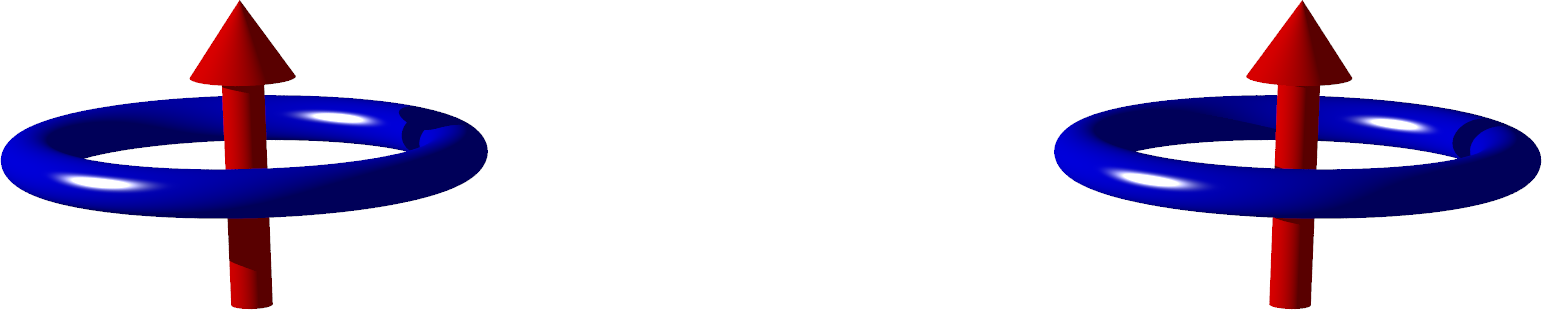
\includegraphics[width=.8\linewidth]{figures/theory/double_torus.png}
\caption[Deux atomes circulaires côte à côte]{Représentation de deux atomes de Rydberg circulaires dont les orbites sont dans le même plan.
Les tores bleus représentent les orbites électroniques et les flèches rouges la direction du moment cinétique.
Si l'on imagine que le dessin est à l'échelle, alors les atomes sont ici séparés d'une distance d'environ \SIv{660}{\nm}.}
\label{fig:double_torus}
\end{figure}
%
Comme il a été dit en \ref{sec:circ_parabol}, les atomes de Rydberg circulaires ont besoin d'un champ électrique extérieur pour se stabiliser.
Nous imposerons donc un champ de \SIvvSym{1}{\V\per\cm}, qui définit l'axe de quantification, parallèle aux flèches rouges sur la figure \eqref{fig:double_torus}.

Les règles de sélection étant toujours valides, le couplage se fait \textit{a priori} à l'ordre deux, et l'équation \eqref{eq:VdW_aacd} permet d'en extraire le coefficient de Van der Waals comme nous l'avons fait pour l'interaction 60S-60S.
Cependant, l'équation \eqref{eq:Vdd_rr1r2} ne prend plus la même forme dans la base parabolique et le moment magnétique total $M$ de la paire atomique n'est plus conservé, ce que doit prendre en compte le calcul numérique.

\begin{figure}[!h]
\centering
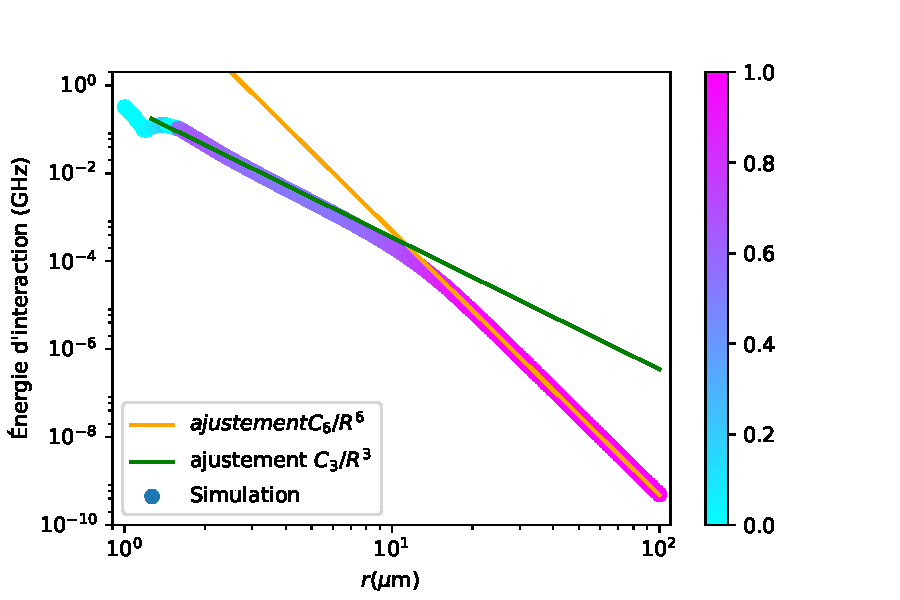
\includegraphics[width=1\linewidth]{figures/theory/VdW_50C50C_1Vcm}
\caption[Interaction dipolaire 50C-50C]{Déplacement en énergie de la paire 50C-50C placés côte à côte (cf fig\eqref{fig:double_torus}) par interaction dipolaire, sous un champ électrique de $\SIvv{1}{\V / \cm}$. L'échelle de couleur représente le carré de la projection sur l'état non perturbé $\ket{50\text{C} 50\text{C}}$ de l'état propre du hamiltonien qui le suit adiabatiquement.
Le comportement dévie franchement de la forme de Van der Waals en $1/r^6$ dès que la distance interatomique est inférieure à $\SIv{10}{\micro\meter}$.
%Aux très courtes distances, le couplage vers d'autres niveaux atomiques devient très fort et l'énergie d'interaction}
}
\label{fig:VdW_50C50C_1Vcm}
\end{figure}

La figure \eqref{fig:VdW_50C50C_1Vcm} présente le résultat du calcul numérique.
Aux grandes distances, l'énergie d'interaction varie bien en $1/r^6$ comme on l'attend, avec un coefficient de Van der Waals 
\begin{equation}
\label{eq:C6_50C50C}
C_{6,50C50C}(\SIvv{1}{V/cm}) = \SIv{483.17}{\GHz\raiseto{6}\um}.
\end{equation}
Mais dès que les atomes se rapprochent à une distance inférieure à $\SIvv{10}{\um}$, l'énergie d'interaction varie en $1/r^3$ jusqu'à très courte distance.
En effet, lorsque l'interaction dipolaire devient suffisamment forte, le champ électrique extérieur ne suffit plus à définir le plan des orbites, et le niveau de paire est perturbé.
C'est ce que l'on retrouve sur la coloration de la courbe : à une distance critique de l'ordre de $\SIvv{10}{\um}$ le niveau de la paire s'éloigne du niveau non perturbé $\ket{\mathrm{50C,50C}}$.
La paire est alors dans un état superposé de plusieurs $\ket{nmk,n'm'k'}$, entre lesquels apparaissent des couplages dipolaires résonants en $1/r^3$.
Ce problème sera traité en détail dans le chapitre \ref{chapter:circsim}, lorsque nous nous intéresserons aux conditions dans lesquelles les interactions entre atomes circulaires sont les plus avantageuses pour la simulation quantique.

Si l'on approche encore les deux atomes, à des distances inférieures à \SIvv{2}{\um}, la base des états propres du hamiltonien de paire devient très différente de la base des états non perturbés.
Il est alors très difficile de décrire simplement l'interaction dipolaire.

\section*{Conclusion}
\noindent Nous avons dans ce chapitre présenté les caractéristiques physiques principales des atomes de Rydberg alcalins.
Nous avons utilisé la théorie du défaut quantique afin de décrire les niveaux de Rydberg de faible moment cinétique.
Ceux-ci dévient en effet du modèle de l'atome d'hydrogène par les effets de pénétration et de polarisabilité du c\oe ur atomique, ce que permet de corriger le défaut quantique.
Ainsi nous avons pu décrire le niveau 60S, en donnant la forme de sa fonction d'onde, sa taille et sa durée de vie radiative à différentes températures.

Nous nous sommes ensuite intéressés aux niveaux de Rydberg circulaires, qui semblent être de meilleurs candidats pour la simulation quantique grâce à leur temps de vie plus long.
La théorie du défaut quantique n'est plus nécessaire pour décrire les niveaux circulaires.
Cependant, l'introduction de la base des états paraboliques est d'une grande aide à leur description, en particulier en présence d'un champ électrique.
Nous avons ainsi pu décrire le niveau de Rydberg circulaire 50C, qui présente un temps de vie à température nulle de presque \SIvv{30}{\ms}.

En dernier lieu, nous avons vu comment les atomes de Rydberg interagissent entre eux par interaction dipolaire.
\`A grande distance, l'interaction dipolaire entre deux atomes de Rydberg prend la forme de Van der Waals avec une dépendance en $C_6/r^6$, où $r$ est la distance entre les deux atomes.
Nous avons pu déterminer les coefficients de Van der Waals $C_6$ pour l'interaction entre une paire d'atomes dans les niveaux $\ket{\text{60S,60S}}$, $\ket{\text{60S,nl}}$ et $\ket{\text{50C,50C}}$, en diagonalisant à chaque fois le hamiltonien complet du système pour toutes les distances $r$.
Aux distances très courtes, lorsque l'interaction dipolaire devient comparable aux différences d'énergie entre les niveaux de Rydberg, les niveaux de Rydberg se mélangent et l'interaction dipolaire ne peut plus être traitée simplement.

Les expériences que nous avons menées portent sur l'étude de l'interaction dipolaire entre atomes de Rydberg.
Il nous a fallu pour cela mettre en \oe uvre un dispositif expérimental que nous présentons dans le prochain chapitre.% \eqref{chapter:setup_coldatoms_Rydberg} .

%Plus particulièrement, nous avons étudié l'interaction dipolaire au sein d'un nuage dense d'atomes dans le niveau 60S, et nous avons 

%Les particularités de l'interaction dipolaire entre niveaux de très grand $l$ sera traitée au chapite \ref{chapter:circsim}.

%------------------------------------------------
%\chapter{Dispositif expérimental : une puce atomique pour des atomes de Rydberg}
%\label{chapter:setup}
\chapter{Des atomes de Rydberg froids en environnement cryogénique}
\label{chapter:setup_coldatoms_Rydberg}
%
%INTRODUCTION DU CHAPITRE\\
%entre autres, longue vie aux Rydberg en environnement cryogénique
\vfill
\minitoc
\newpage

\noindent L'observation d'atomes de Rydberg en interaction sur des temps longs, tant pour la question du mouvement d'un gaz de Rydberg ultra-froids que dans l'optique de la simulation quantique, requiert des conditions expérimentales spécifiques.
D'une part, il est souhaitable que la durée de vie des niveaux de Rydberg soit la plus longue possible, ce qui nous pousse à travailler en environnement cryogénique.
Les calculs menés dans le chapitre \ref{chapter:Rydberg} nous montrent l'importance de la température de l'environnement sur la durée de vie des atomes de Rydberg, plus cruciale encore si l'on souhaite travailler avec des atomes de Rydberg circulaires.

D'autre part, il est nécessaire, étant donnés nos objectifs, que nos atomes de Rydberg soient aussi froids que possible.
L'on pourrait imaginer piéger et refroidir des atomes qui auraient été préalablement excités dans des niveaux de Rydberg à partir d'un jet atomique chaud.
Cependant, il n'y a pas de technique connue à ce jour qui permette cela, et la durée de vie des niveaux de Rydberg en limiterait très certainement les possibilités.
Or les techniques de piégeage et de refroidissement des atomes alcalins non excités sont des outils bien maîtrisés.
Voilà donc une piste bien plus prometteuse.

Une première difficulté se présente ici : les techniques d'atomes ultra-froids sont pour la plupart développées au sein de dispositifs à température ambiante.
Il s'agira donc ici de les concilier avec un environnement cryogénique.
Avec cette contrainte à l'esprit, et dans l'optique d'obtenir des nuages atomiques très confinés, il a été choisi de centrer le dispositif autour d'une puce à atomes supraconductrice.
Prenons note dès maintenant d'une deuxième difficulté technique posée par un tel dispositif :
les atomes de Rydberg sont extrêmement sensibles au champ électromagnétique, et nous souhaitons les exciter et les observer au voisinage de la surface conductrice qu'est notre puce atomique.

Ce chapitre sera donc dédié à la description du dispositif expérimental sur lequel nous avons effectué nos travaux.
Nous nous intéresserons d'abord à l'aspect du dispositif qui nous sert à piéger et refroidir des atomes de \Rb{87} sur une puce atomique supraconductrice.
Nous nous attacherons ensuite à décrire comment nous excitons, manipulons et détectons les atomes de Rydberg au sein de ce dispositif.

%\clearpage
\section{Un nuage d'atomes ultra-froids sur puce, du MOT de capture au condensat de Bose-Einstein}
\noindent Le développement de notre plateforme d'atomes froids autour d'une puce supraconductrice a été l'objet de plusieurs thèse de doctorat précédant celle-ci.
Les thèses de Thomas Nirrengarten \cite{PHD_NIRRENGARTEN}, de Cédric Roux \cite{PHD_ROUX} et d'Andreas Emmert \cite{PHD_EMMERT} sont dédiées à la question du piégeage et du refroidissement jusqu'au BEC d'atomes de \Rb{87} près d'une surface à l'aide de fils supraconducteurs.
La thèse de Raul Celistrino Teixeira \cite{PHD_CELISTRINO} détaille la fabrication et les caractéristiques de la puce atomique que nous avons utilisée pour nos expériences.

Nous ferons donc ici une présentation rapide du cryostat et de la puce à atomes que nous utilisons, puis nous détaillerons la suite d'étapes que nécessite le piégeage et le refroidissement des atomes de rubidium au sein de notre dispositif.
Enfin, après avoir présenté la technique d'imagerie atomique par absorption, nous présenterons quelques chiffres typiques de nos nuages atomiques.


\subsection{L'environnement cryogénique : cryostat et puce à atomes supraconductrice}\label{subsec:cryopuce}
\noindent L'environnement cryogénique présente un avantage incomparable pour la durée de vie des atomes de Rydberg, mais impose aussi quelques spécificités à notre dispositif d'atomes froids.
Le piégeage d'atomes froids pendant des durées suffisantes à leur manipulation exige un vide très poussé dans l'enceinte expérimentale, car les collisions avec les molécules de gaz résiduel éjectent les atomes hors de leur piège.
Les chambres de piégeage d'atomes neutres à température ambiante sont généralement étuvées pendant plusieurs semaines afin d'atteindre des pressions de gaz résiduel suffisamment faibles.
Dans un environnement cryogénique au contraire, les parois froides de l'enceinte adsorbent une grande partie du gaz résiduel, et des pressions très inférieures à \SIvv{1e-10}{\milli\bar} sont obtenues sans étuvage.
Travailler en environnement cryogénique permet en outre l'utilisation de fils et de bobines supraconducteurs pour le passage des courants électriques qui génèrent les champs magnétiques nécessaires au piégeage des atomes.
Des courants de quelques Ampères sont ainsi passés sans dissipation et à proximité des atomes piégés, alors qu'une expérience d'atomes froids à température ambiante nécessite des bobines qui soient placées en-dehors de la chambre et refroidies par des circuits d'eau dédiés.

L'environnement cryogénique pour les atomes froids a cependant quelques inconvénients :
en premier lieu, l'accès optique est limité car les parois de l'enceinte doivent être opaques pour le rayonnement du corps noir et donc métalliques, chaque hublot de verre réduisant l'isolation thermique du c\oe ur de l'expérience.
En second lieu, l'utilisation d'hélium et d'azote liquide à proximité d'un vide poussé présente une lourdeur technique supplémentaire au quotidien.

\subsubsection*{Le cryostat}
\noindent Notre expérience est placée au c\oe ur du cryostat représenté en figure \eqref{fig:cryo}.
%
\begin{figure}
\centering
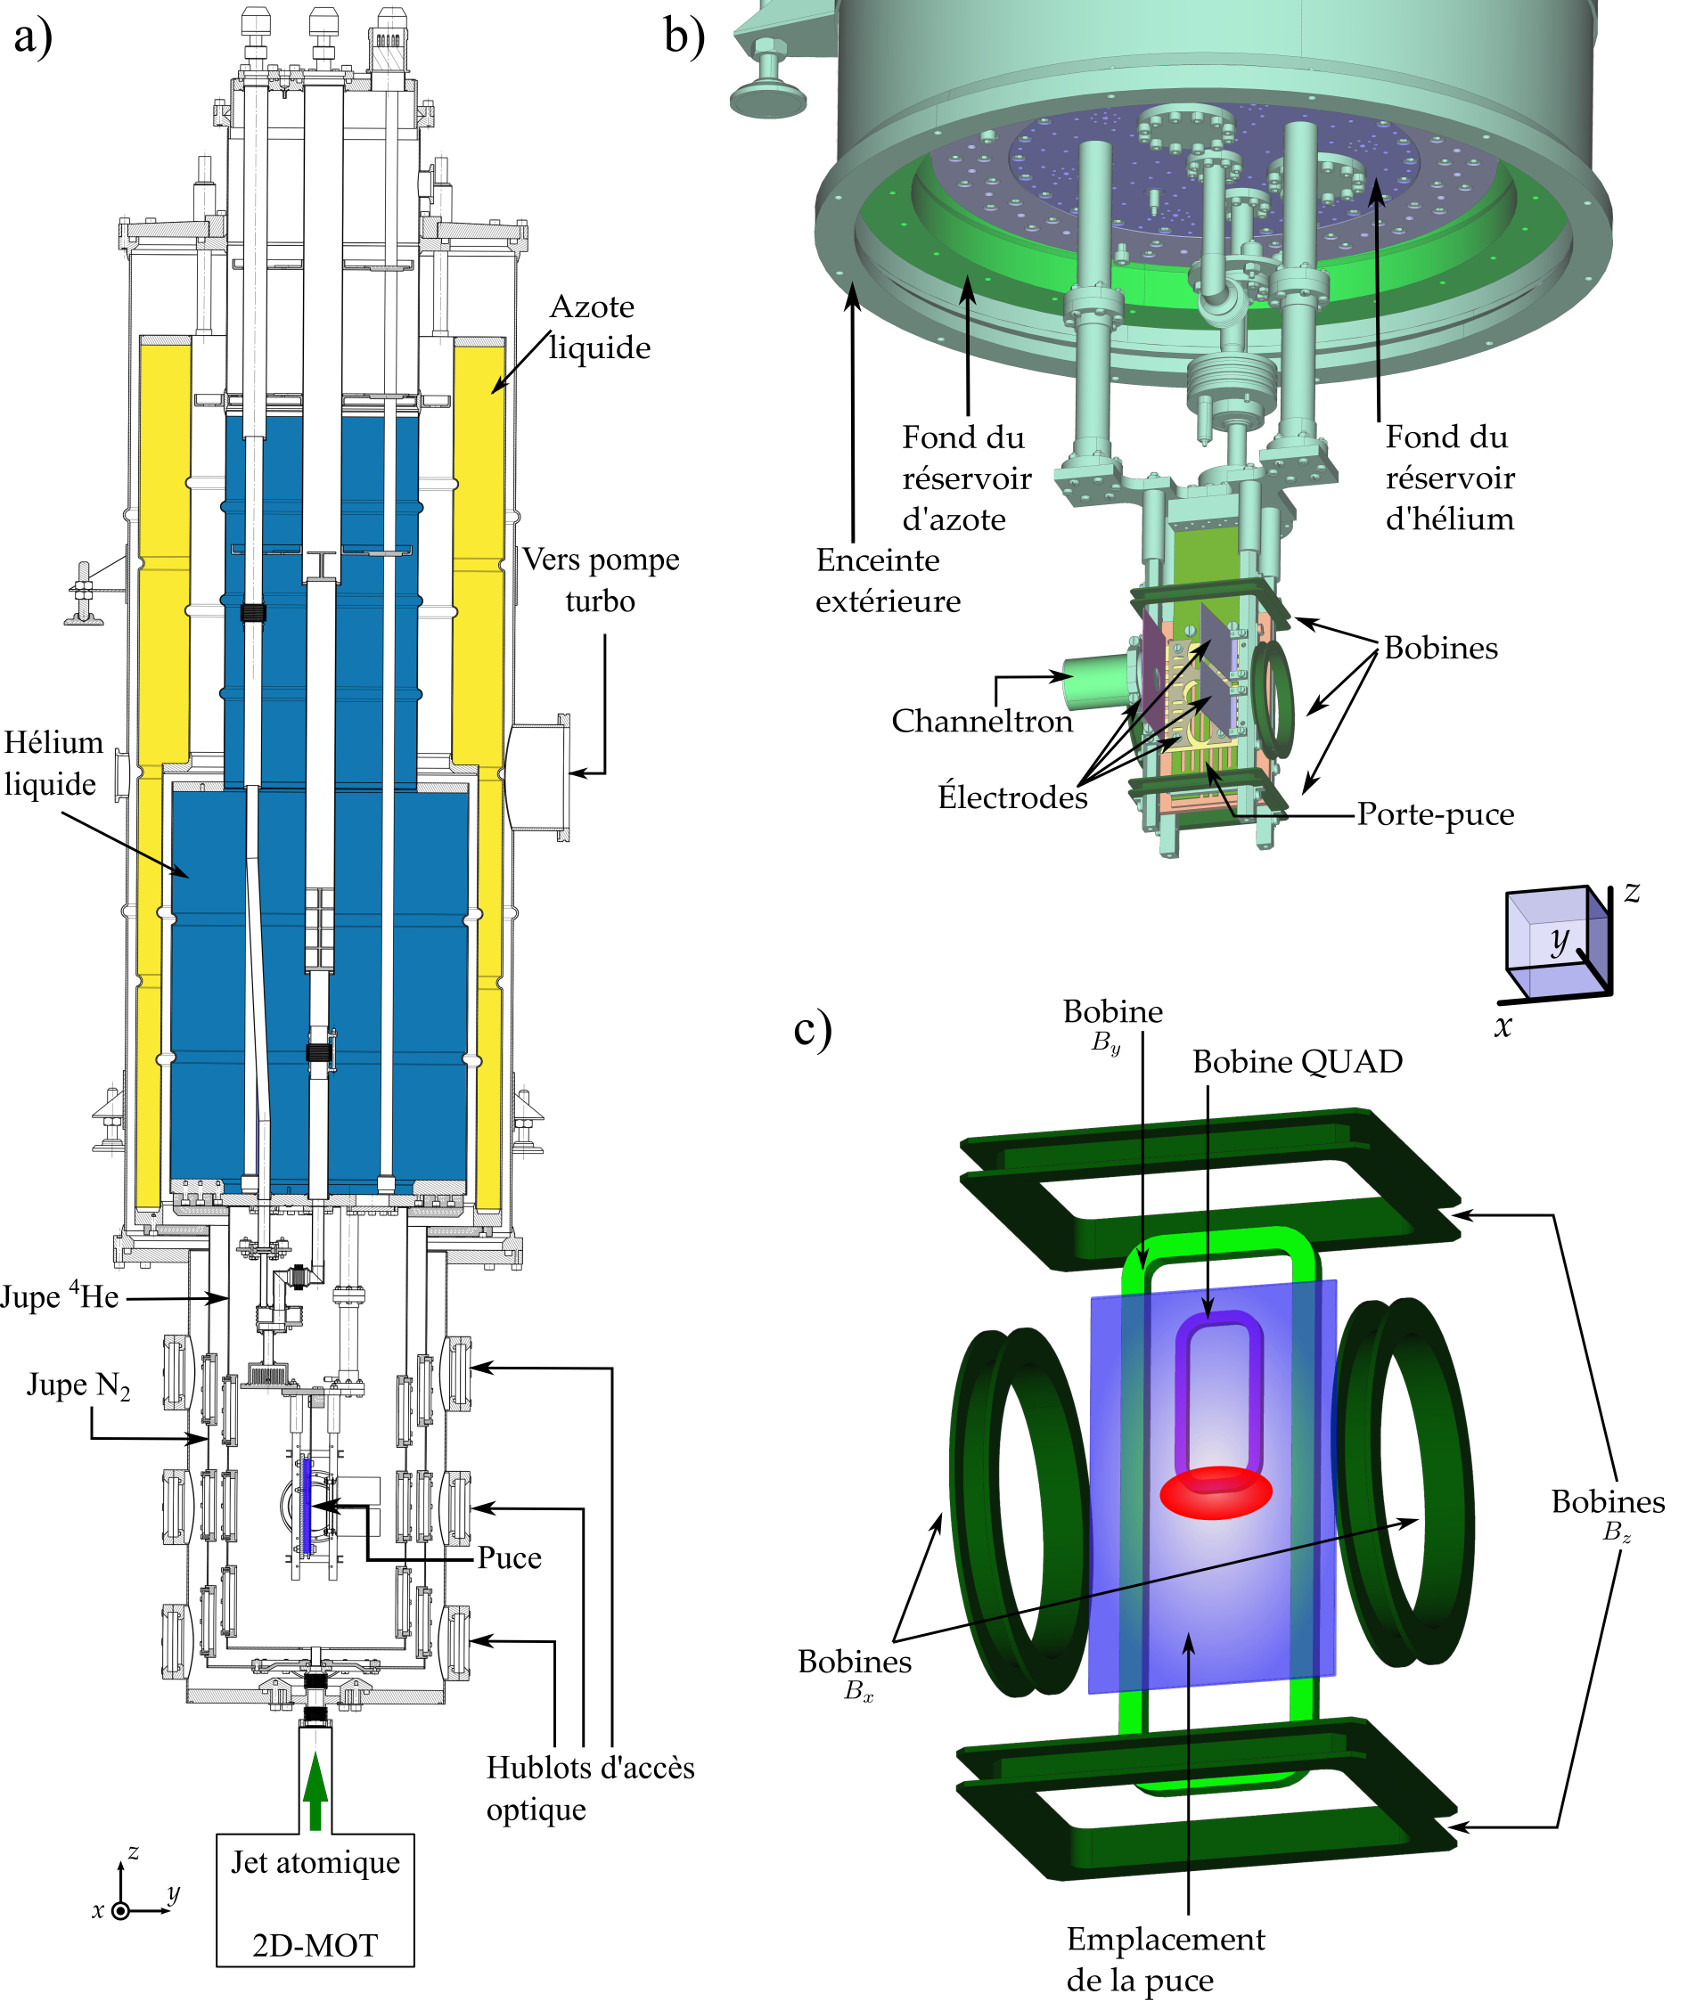
\includegraphics[width=\linewidth]{figures/setup/coldatoms/cryo_vect2.jpg}
\caption[Schéma du cryostat]{Schéma du dispositif cryogénique :
\textbf{a)} Coupe du du cryostat, avec la puce (colorée en violet) tournée vers le côté droit.
Le réservoir d'azote liquide est indiqué en jaune, le réservoir d'hélium liquide en bleu.
Le c\oe ur de l'expérience est visible, ainsi que les deux \og jupes \fg{} et l'enceinte extérieure à température ambiante.
Cinq hublots, trois en face de la puce et un sur chaque côté, sont installés sur chacune de ces jupes pour l'accès optiques.
Derrière la puce, du côté gauche du schéma, les hublots optiques sont remplacés par des disques métalliques.
Les atomes proviennent du \og 2D-MOT \fg{}, une enceinte externe située sous le cryostat, où l'on réalise un piège magnéto-optique à deux dimensions.
\textbf{b)} Vue schématique du c\oe ur de l'expérience. La puce est fixée sur le porte-puce et fait face à la direction $y$. Les bobines (vert foncé) servent à créer des champs magnétiques pour le piégeage des atomes de rubidium.
Le channeltron et les différentes électrodes représentées servent à la détection des atomes de Rydberg. On ne voit pas les \og jupes \fg{} d'azote et d'hélium, ni l'enceinte extérieure.
\textbf{c)} Vue de près des bobines : la bobine QUAD (mauve) génère un champ quadrupolaire pour faire un MOT sur puce. L'emplacement de la puce est représenté par le rectangle bleu devant la bobine QUAD et la bobine $B_y$ (vert clair).
La zone rouge indique l'endroit où les atomes de rubidium sont piégés, devant la puce.
Les axes sont les mêmes qu'en \textbf{b)}.
}
\label{fig:cryo}
\end{figure}
%
La conception de ce cryostat a été évoquée dans la thèse de Raul Celistrino Teixeira \cite{PHD_CELISTRINO}  et discutée plus en détail dans les thèses de Thomas Nirrengarten \cite{PHD_NIRRENGARTEN} et Cédric Roux \cite{PHD_ROUX}.
Le c\oe ur de l'expérience est protégé de la radiation extérieure par des écrans thermiques (\og jupes \fg{}) en cuivre doré. Ce sont des cylindres ouverts en haut et vissés sur le fond des réservoirs de liquides cryogéniques.
La jupe $^4 \text{He}$ est vissée sur le fond du réservoir d'hélium 4 et la jupe $\text{N}_2$ est vissée au fond du réservoir d'azote liquide.
Elles sont donc respectivement thermalisées à \SIvv{4.2}{\K} et \SIvv{77}{\K}.
Sur chaque jupe, cinq hublots sont installés pour l'accès optique à la zone de piégeage :
deux sur les directions $\pm x$, un dans la direction $+y$ qui fait face à la puce, et deux  dans le plan $yz$, de part et d'autre du hublot de face sur les bissectrices des axes $+y$ et $\pm z$, appelées direction $\pm\SIvv{45}{\degree}$ respectivement.
Par ces hublots, tous les faisceaux laser atteignent la zone de piégeage au c\oe ur de l'expérience.
Tous les éléments qui sont installés à l'intérieur de la jupe hélium sont thermalisés à \SIvv{4.2}{K} par contact thermique avec le réservoir d'hélium liquide.

L'intérieur de la jupe hélium est revêtu d'une couche de plomb, supraconducteur à \Khe. Cette couche de plomb écrante les champs magnétiques extérieurs par effet Meissner \cite{MX_MEISSNEREFFECT}, et évite les courants de Foucault qui se créeraient dans les jupes en cuivre à l'allumage ou à l'extinction des courants dans les bobines. 
Il reste nécessaire cependant d'imposer un champ extérieur de compensation au moment du refroidissement, afin que la couche de plomb ne piège pas de lignes de champ magnétique provenant de l'environnement.
Cette compensation du champ constant de l'environnement est réalisée à l'aide de grandes bobines placées à l'extérieur du crysotat.

Enfin, bien que les jupes ne soient pas parfaitement étanches, elles garantissent un vide différentiel entre la partie du cryostat à \SIvv{300}{\K}, où la pression vaut \SIvv{1.5e-7}{\milli\bar}, et la partie à \Khe, où la pression est inférieure à \SIvv{1e-10}{\milli\bar}\footnote{
Cette valeur n'est pas mesurée en raison de l'absence de sonde de pression dans cette région du cryostat, mais inférée à partir du temps de vie des nuages d'atomes piégés, qui est de l'ordre de la minute \cite{ENS_CHIPLIFETIME}.}.

%\clearpage
\subsubsection*{La puce à atomes}
\noindent La puce à atome qui siège au c\oe ur de notre expérience est représentée en figure \eqref{fig:chip}.
C'est une puce assez simple, conçue autour de trois fils supraconducteurs : le fil (LJ), en forme de \mcal{U}, le fil (LG) en forme de \mcal{Z}, et le fil (KM) droit.
Ces fils sont fabriqués par dépôt de niobium d'une épaisseur de \SIvv{2}{\um} sur un substrat de silicium recouvert d'une couche d'oxyde SiO$_2$.
Le dépôt de niobium est ensuite gravé, et l'ensemble de la puce est recouvert d'une couche d'or de \SIvv{200}{\nm} d'épaisseur afin de rendre la surface réfléchissante.
Le niobium étant supraconducteur à $\SI{4.2}{\K}$, les courants électrique pourront toujours passer par les fils de la puce et non par la couche d'or qui reste dans un de état conducteur normal.
Les détails de la fabrication de la puce sont présentés en annexe dans la thèse de Raul Celistrino Teixeira \cite{PHD_CELISTRINO}.
%
\begin{figure}[!h]
\centering
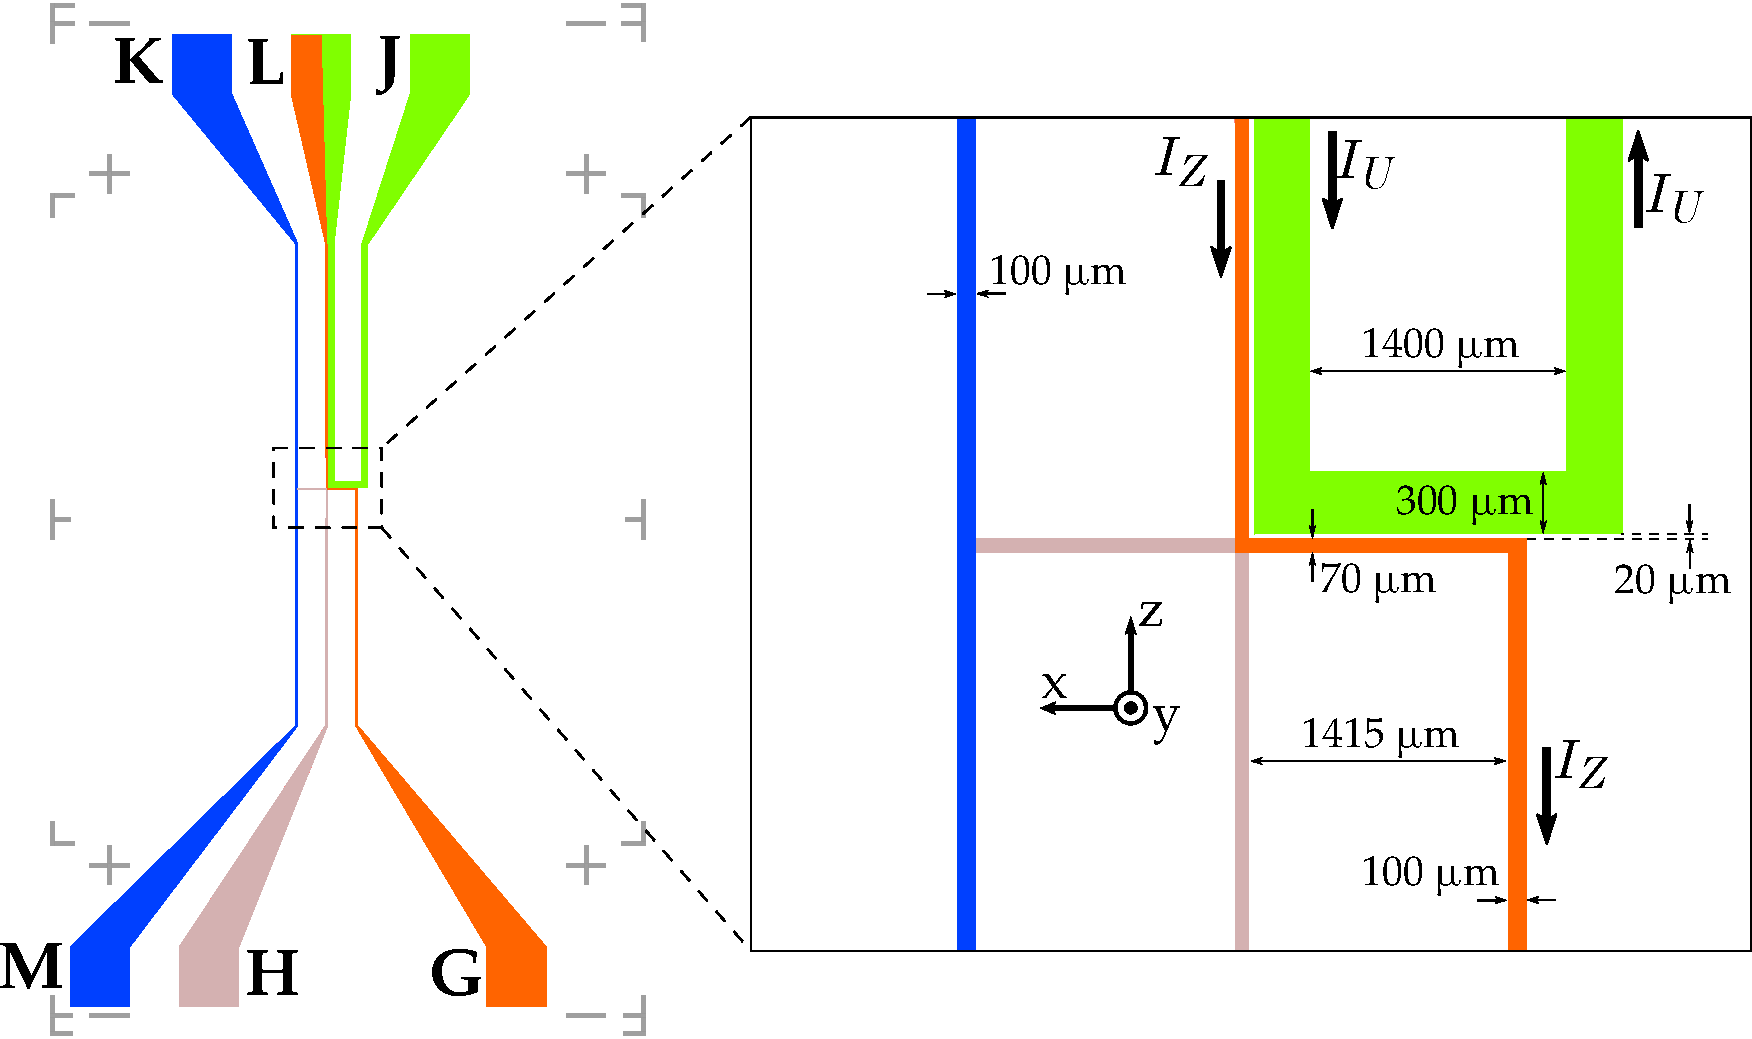
\includegraphics[width=\linewidth]{figures/setup/coldatoms/chip}
\caption[Schéma de la puce à atomes supraconductrice]{Schéma de la puce supraconductrice.
Les lettres étiquettent les pattes d'entrée/sortie des courants électriques sur la puce.
Les couleurs sont une aide visuelle pour mieux suivre les fils : en vert, le \og fil \mcal{U}\fg{}, en orange le \og fil \mcal{Z}\fg{} et en bleu le \og fil RF \fg{}.
\`A droite, vue de près du centre de la puce, qui détaille la largeur des fils, la distance entre eux et le sens de circulation des courants.
Les axes $x,y$ et $z$ coïncident avec ceux de la figure \eqref{fig:cryo}.
}
\label{fig:chip}
\end{figure}
%

Les fils en \mcal{U} et en \mcal{Z} sont la simplification d'un dispositif en forme de $\mathcal{H}$ qui repose sur la circulation d'un premier courant perpendiculairement à deux autres courants qui sont parallèles entre eux.
La figure \eqref{fig:magfields_chip} représente les différentes configurations de champ magnétique créées par les fils \mcal{U} et \mcal{Z} de la puce.

Le passage d'un courant dans la partie horizontale du fil \mcal{U}(segment parallèle à l'axe $x$) crée un champ contenu orienté dans le plan $yz$, que l'on peut approximer au champ créé par un fil infini.
L'ajout d'un champ de biais $B_z$ selon l'axe $z$ permet alors de créer un zéro de champ, là où le champ de biais compense exactement le champ créé par le fil.
Autour de ce zéro, le champ magnétique est quadrupolaire dans le plan $yz$ (cf figure \ref{fig:magfields_chip}b)).
Afin de compléter ce champ quadrupolaire dans la direction $x$, un courant parcourt les bras verticaux du fil en \mcal{U} : le sens opposé de circulation dans ces deux bras crée directement un champ quadrupolaire dans la direction $x$ avec un minimum nul (cf figure \ref{fig:magfields_chip}d)).
La composante de champ résiduelle selon $y$ est compensée par un champ de biais $B_y$.
En fin de compte, le champ magnétique présente un comportement quadrupolaire dans les trois directions, autour d'un minimum nul dans les trois directions.
Le champ total permet ici la réalisation d'un piège magnéto-optique sur puce en trois dimensions (\og 3D-MOT miroir\fg{}).

Lors du passage d'un courant $I$ dans le fil \mcal{Z}, le champ créé dans le plan $yz$ est similaire au cas du fil en \mcal{U}.
Cependant, le courant dans les deux bras verticaux circule dans le même sens et crée ainsi un champ quadrupolaire dans le plan $xy$.
Le champ magnétique présente donc aussi un comportement quadrupolaire dans les trois directions, mais autour d'un minimum qui est cette fois non-nul (cf figure \ref{fig:magfields_chip}c)).
Le champ total forme alors un piège magnétique de Ioffe-Pritchard.

\begin{figure}[!h]
\centering
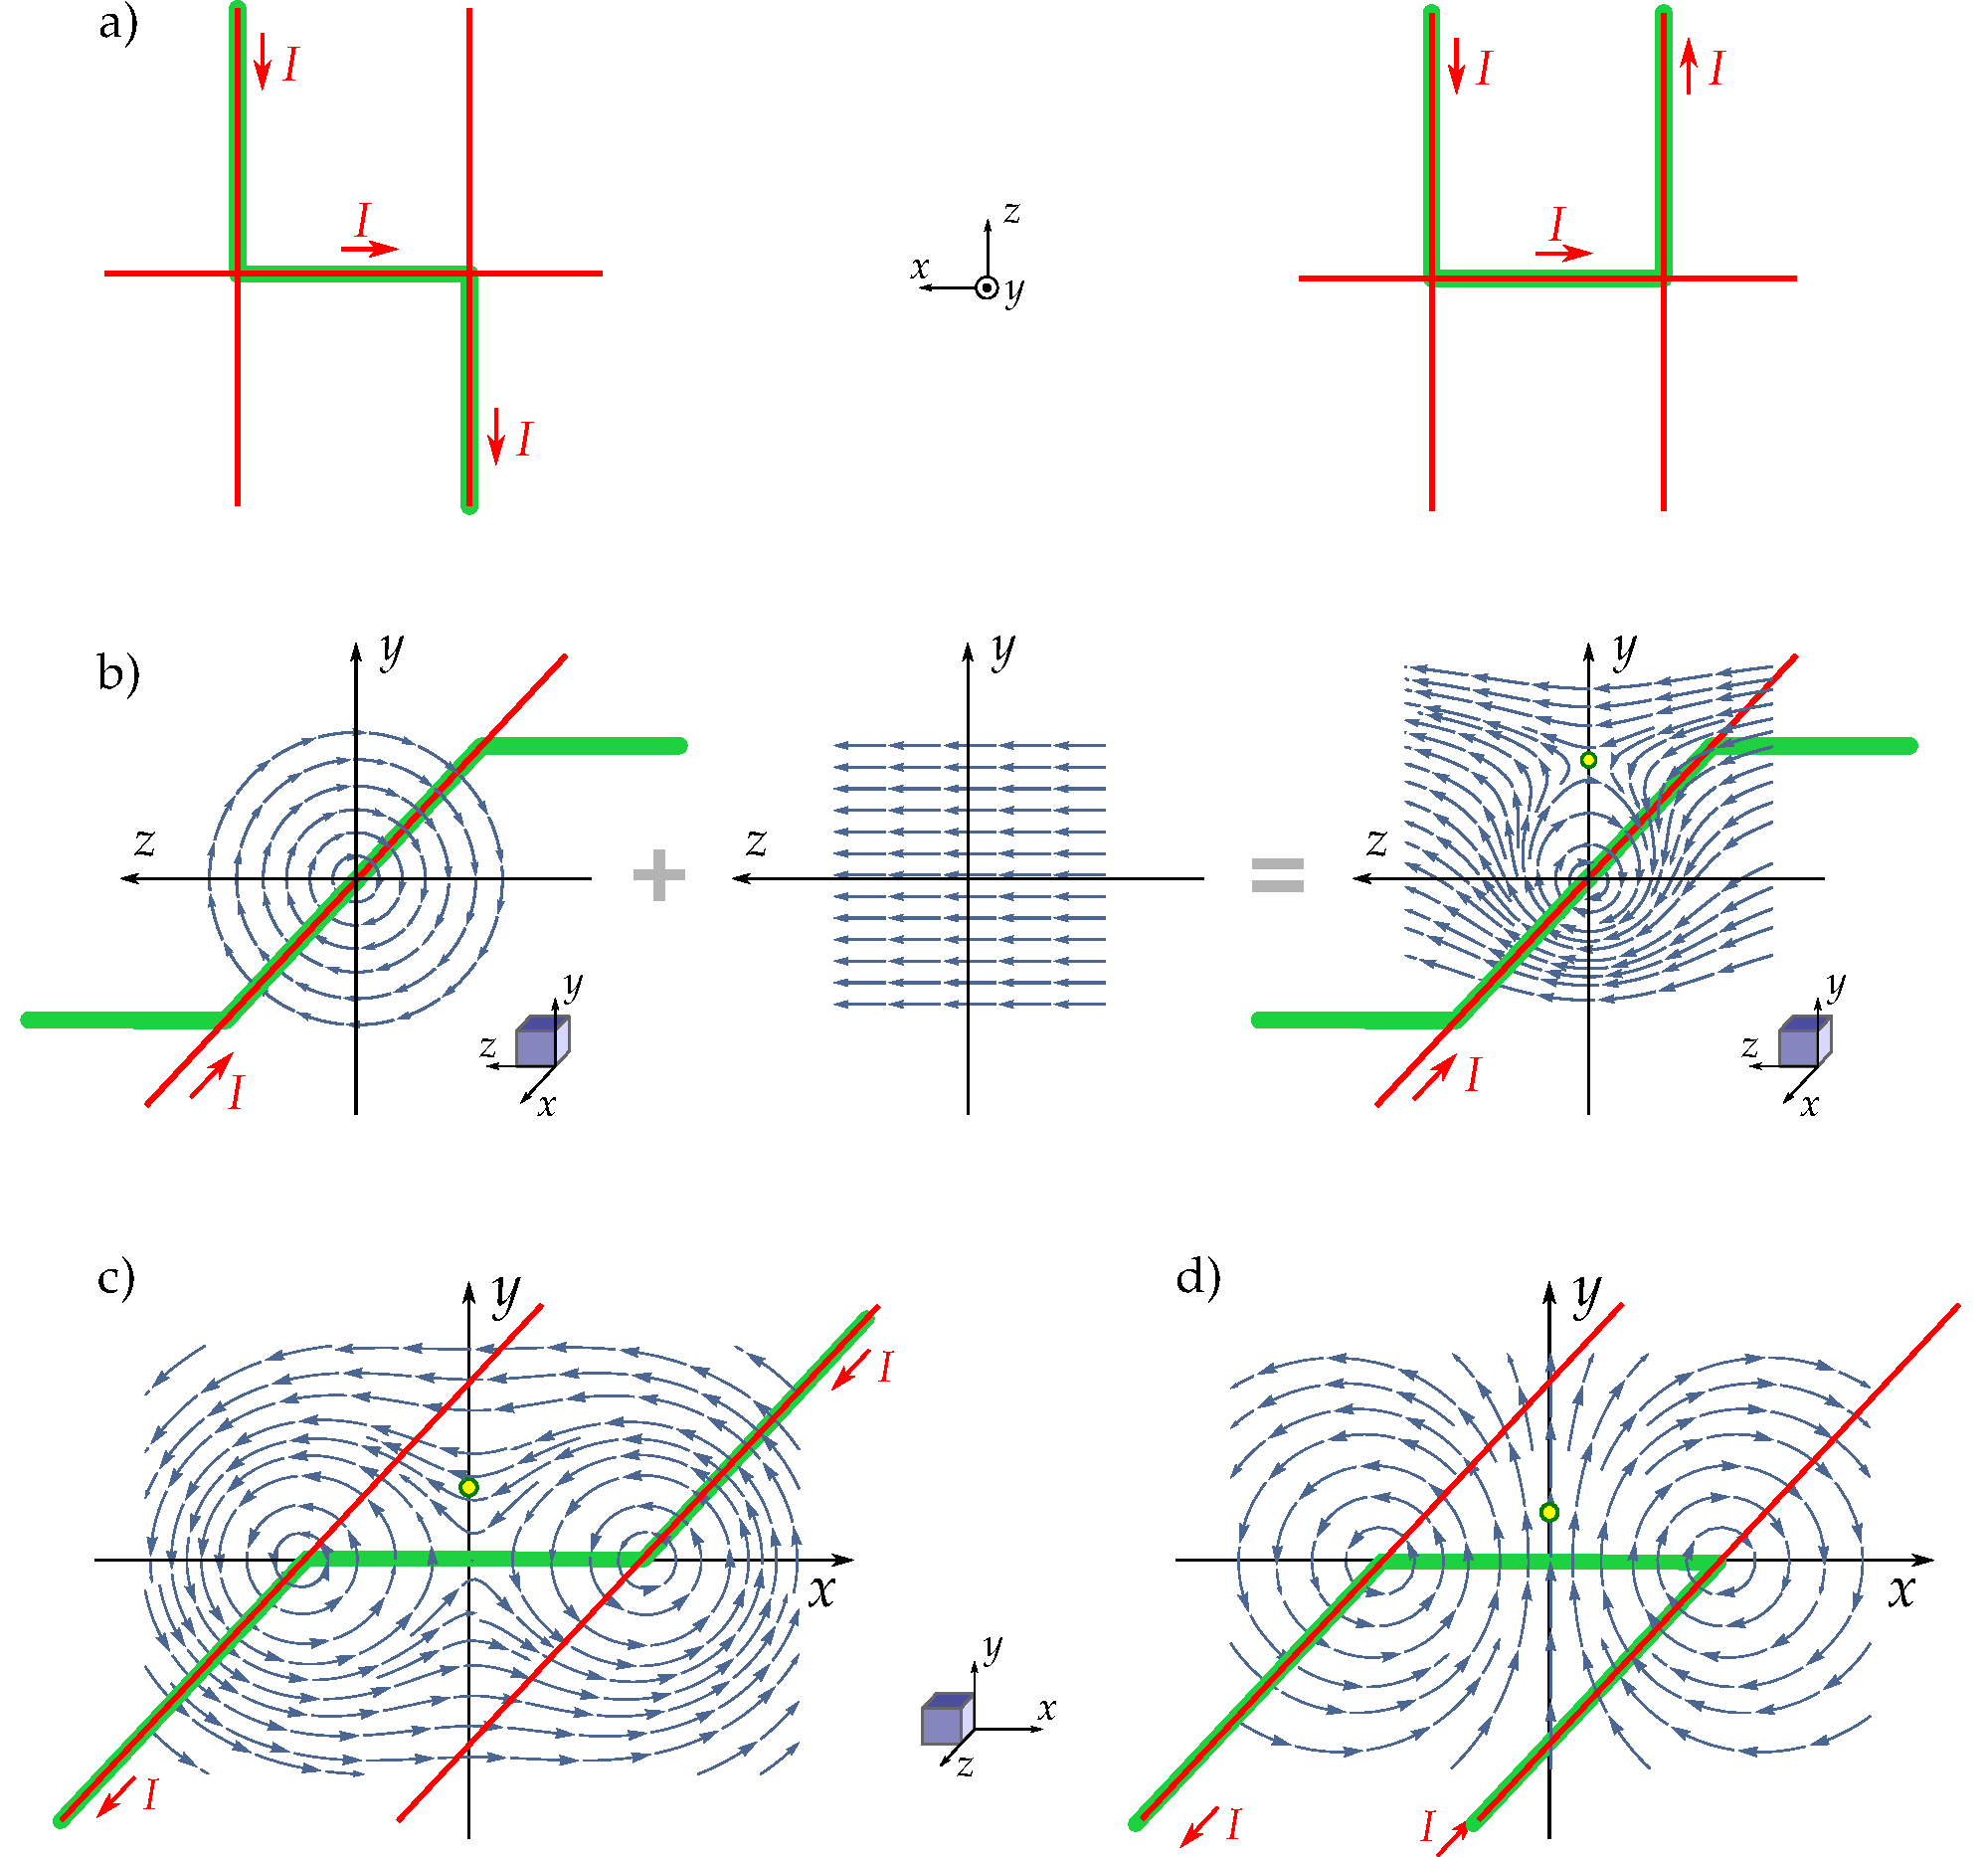
\includegraphics[width=\linewidth]{figures/setup/coldatoms/magfields_chip}
\caption[Champs magnétiques créés par la puce]{
Champs magnétiques créés par la puce.
\textbf{a)} Les fils \mcal{U} et \mcal{Z} portent un courant dans la direction $x$ et une paire de courants parallèles dans la direction $z$.
\textbf{b)} Un champ quadrupolaire est créé par la superposition du courant selon $x$ et d'un champ de biais $B_Z$.
Les courants verticaux peuvent circuler soit (\textbf{c)}) dans le même sens,  soit (\textbf{d)}) dans des sens opposés.
Le module du champ total présente alors respectivement un minimum non-nul ou nul aux positions marquées par les points jaunes.
}
\label{fig:magfields_chip}
\end{figure}

Pour le fil en \mcal{Z} comme pour le fil en \mcal{U}, le centre du piège se situe à une distance de la puce valant approximativement
\begin{equation}
\label{eq:trap_center}
r_0 \simeq \frac{\mu _0}{2\pi}\frac{I}{B_Z}
\end{equation}
et le gradient de champ magnétique à cet endroit vaut
\begin{equation}
\label{eq:trap_center_grad}
|B'(r_0)|=\frac{2\pi}{\mu _0} \frac{B_Z^2}{I} = \frac{B_Z}{r_0} = \frac{\mu _0}{2\pi}\frac{I}{r_0^2}~.
\end{equation}
%
C'est là une caractéristique importante de la géométrie des pièges : plus le centre du piège est proche de la puce, plus le piège sera confinant dans le plan $yz$.
Le piège s'allonge alors dans la direction $x$, prenant une forme de cigare de plus en plus anisotrope.

\clearpage
Comme nous l'avons mentionné, notre dispositif nous permet de mettre en \oe uvre des pièges magnéto-optiques en trois dimensions.
Dans beaucoup d'expériences d'atomes froids, ceux-ci sont réalisés à l'aide de trois paires de faisceaux laser contra-propageants, une dans chaque direction de l'espace.
Il nous est impossible d'envisager cette configuration, puisque l'axe $y$ est rendu inaccessible par la présence de la puce.
L'on peut cependant, avec deux paires de faisceaux laser seulement, simuler une configuration à six faisceaux, en utilisant la surface réfléchissante de la puce.
Deux faisceaux sont alors envoyés parallèlement à la surface de la puce, selon l'axe $x$.
Deux autres faisceaux sont envoyés dans le plan $yz$ et viennent se réfléchir sur la puce avec un angle de $\SI{45}{\degree}$.
Ces réflexions sont équivalentes aux deux faisceaux manquants, réalisant ainsi la configuration à six faisceaux souhaitée.
Le schéma de cette configuration, appelée \og MOT miroir \fg{}, est donné en figure \eqref{fig:mirror_MOT}.

\begin{figure}[h]
\centering
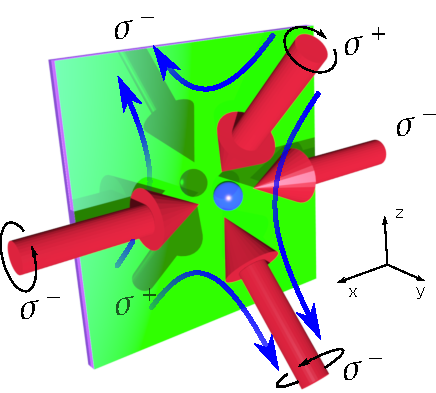
\includegraphics[width=0.6\linewidth]{figures/setup/coldatoms/mirror_MOT}
\caption[Schéma de principe du MOT miroir]{Schéma de principe du MOT miroir :
Deux faisceaux contra-propageants sont envoyés parallèlement à la puce réfléchissante, selon l'axe $x$.
Les deux autres faisceaux dans le plan $yz$ viennent frapper la puce avec un angle de \SIvv{45}{\degree}.
Leur réflexion sur la puce équivaut à deux faisceaux supplémentaires d'hélicité inversée, représentés en ombre derrière la puce.
On obtient bien ainsi une configuration de MOT à six faisceaux, avec les polarisations adaptées, représentées par des flèches tournant autour des faisceaux.
}
\label{fig:mirror_MOT}
\end{figure}


%\clearpage
\subsection{Séquence de piégeage et refroidissement}\label{subsec:exp_seq}
\noindent Grâce à ce dispositif, nous pouvons piéger des nuages d'atomes froids sur puce.
Nous donnons dans ce paragraphe le détail des différentes étapes de piégeage et de refroidissement des atomes.
Les atomes sont envoyés dans le cryostat à partir d'un piège magnéto-optique à deux-dimensions externe, puis ils sont capturés dans deux pièges magnéto-optiques sur puce successifs.
Enfin, les atomes sont transférés dans un piège magnétique pour y être refroidis par évaporation.
L'ensemble de cette séquence est représentée en figure \ref{fig:exp_sequence}.
%	
\begin{sidewaysfigure}
\centering
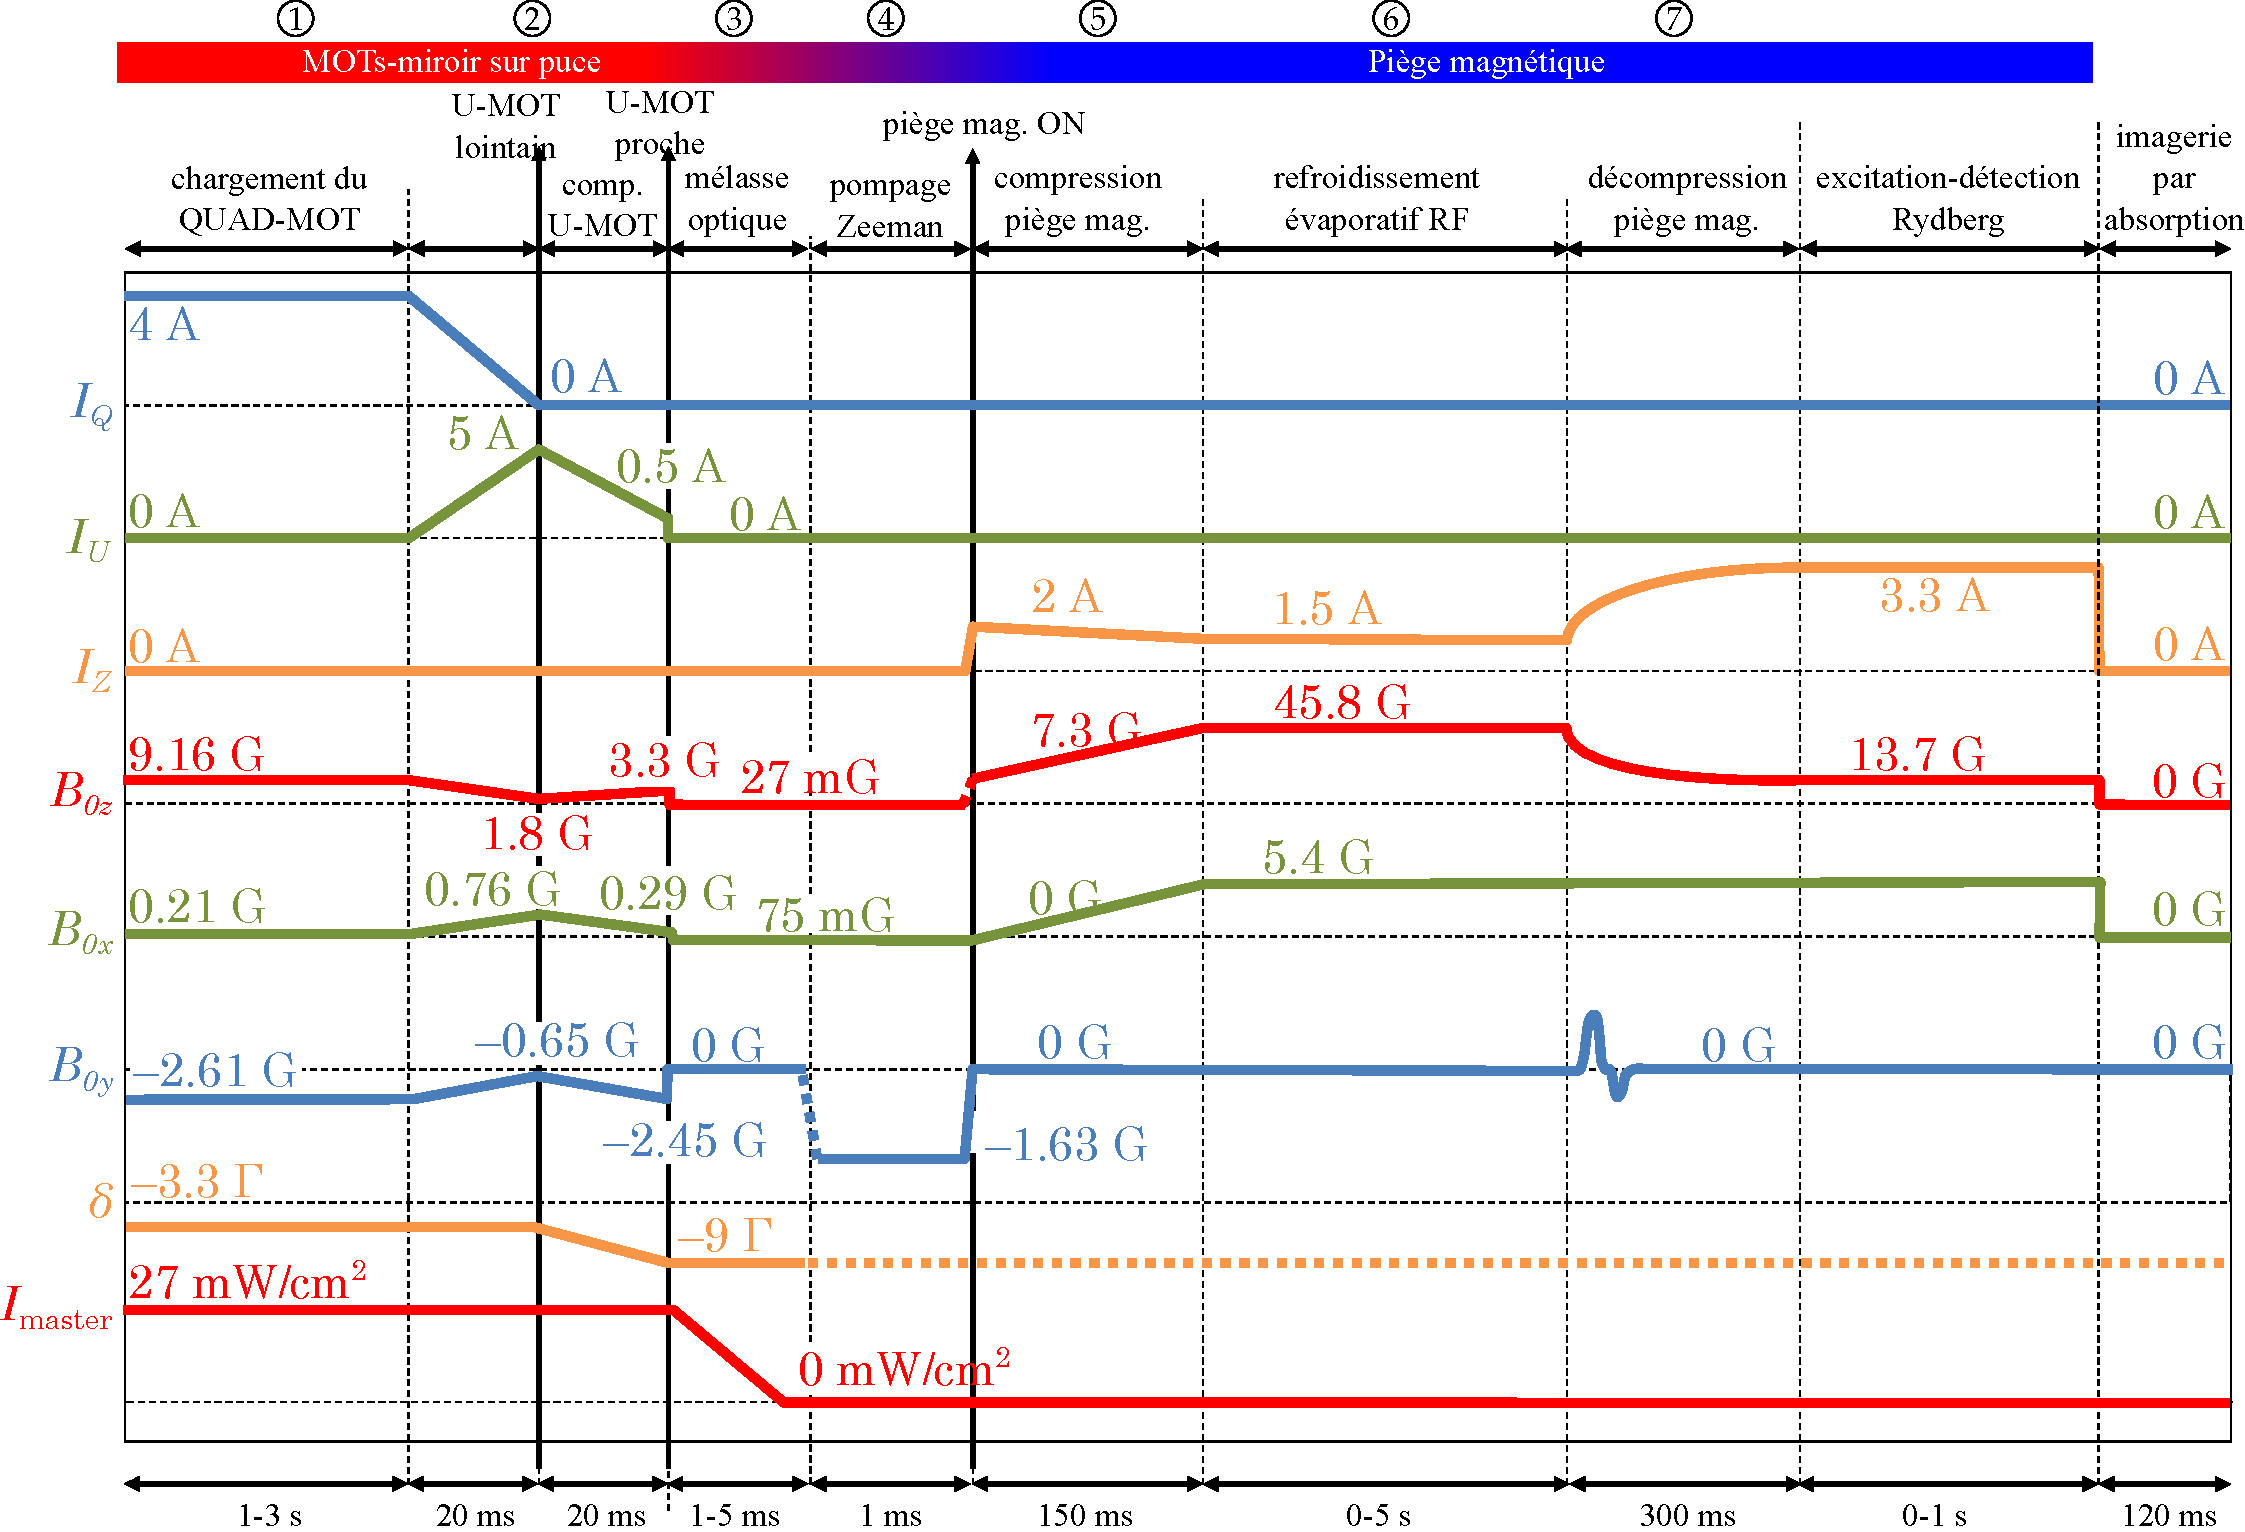
\includegraphics[width=\linewidth]{figures/setup/coldatoms/exp_sequence}
\caption[Séquence expérimentale typique]{Séquence expérimentale typique.% : la durée et les valeurs des paramètres à chaque étape sont précautionneusement optimisés.
Les étapes de piégeage et de refroidissement sont %numérotées de \numrange{1}{7} et 
discutées dans le texte.
Les étapes ultérieures seront décrites par la suite.
$I_{Q,U,Z}$ sont les courants dans la bobine QUAD, le fil \mcal{U} et le fil \mcal{Z}, en Ampères.
$B_{0~x,y,z}$ sont les champs de biais générés par les bobines dans les directions $x,y,z$, en Gauss.
$\delta$ est le désaccord du laser en unité de la largeur de raie $\Gamma=\SI{6.065}{\MHz}$, et $I_{master}$ son intensité en \si[per-mode=symbol]{\milli\watt \per\squared\cm}.
}
\label{fig:exp_sequence}
\end{sidewaysfigure}


\clearpage
\subsubsection*{Système laser}
\noindent Le piégeage magnéto-optique du rubidium 87 exploite la raie D2 de celui-ci.
La raie D2 est représentée en figure \eqref{fig:D2lineRb87} avec le détail des sous-niveaux hyperfins des niveaux $\mathrm{5S_{1/2}}$ et $\mathrm{5P_{3/2}}$ du \Rb{87}.
%	
\begin{figure}[t]
\centering
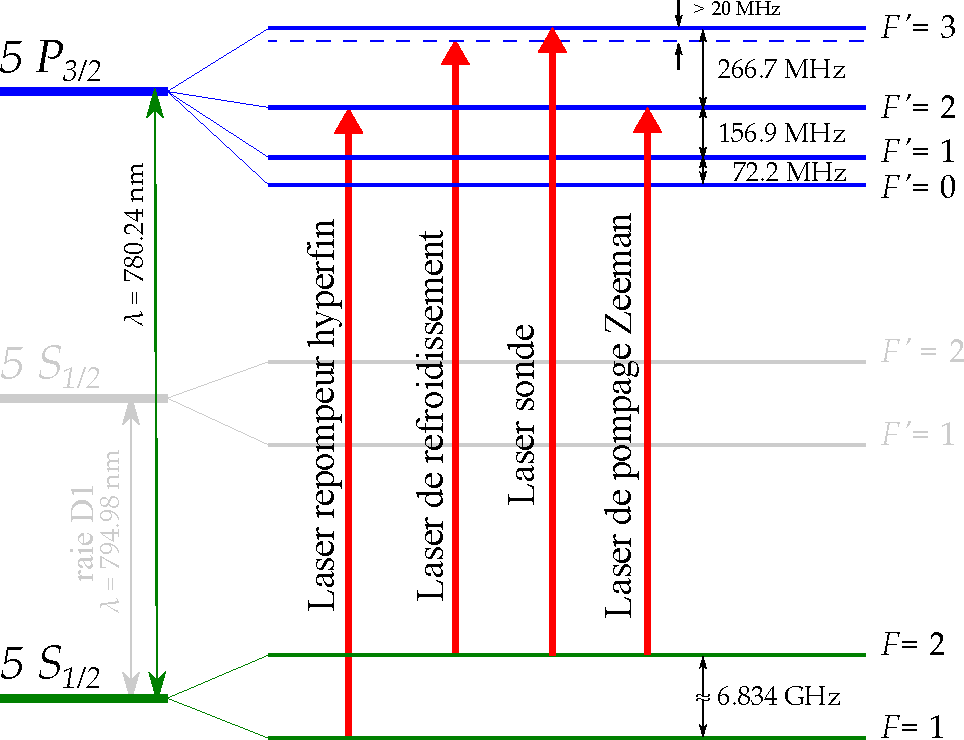
\includegraphics[width=0.8\linewidth]{figures/setup/coldatoms/D2lineRb87}
\caption[Raie D2 du \Rb{87}]{Structure hyperfine de la raie D2 du \Rb{87}.
Les transitions cyclantes sont montrées pour le laser de refroidissement, le laser repompeur, le laser sonde et le laser de pompage Zeeman.
}
\label{fig:D2lineRb87}
\end{figure}
%
Nous utilisons la transition $\ket{F=2} \rightarrow \ket{F'=3}$ de la raie D2 pour piéger et refroidir les atomes.
Cette transition a une largeur naturelle $\Gamma = 2\pi \times \SI{6.065}{\MHz}$ \cite{DATA_STECKRB87}.
Le laser de refroidissement est généré par un système commercial de diode laser amplifiée TOPTICA TA 100.
La fréquence de ce laser est asservie par battement (\og beatlock \fg{}) à un laser maître, lui-même stabilisé par une cavité Fabry-Pérot.
Cette cavité est verrouillée en fréquence sur la transition de refroidissement par absorption saturée dans une cellule de \Rb{87}.
Une commande de tension permet de définir la fréquence du battement et ainsi de contrôler le désaccord du laser de refroidissement par rapport à la transition $\ket{F=2}\rightarrow\ket{F'=3}$.
Le système de stabilisation et de distribution des faisceaux laser de piégeage et de refroidissement est détaillé en annexe \ref{app:laserlock}.

Il arrive qu'un photon du laser de refroidissement excite un atome du niveau $\ket{F=2}$ vers le niveau $\ket{F'=2}$ au lieu de $\ket{F'=3}$.
Cet atome peut alors se désexciter non pas vers le niveau $\ket{F=2}$ mais vers le niveau $\ket{F=1}$, qui est un niveau noir pour le laser de refroidissement.
Afin d'éviter le pompage des atomes vers ce niveau $\ket{F=1}$, il est nécessaire d'envoyer, avec le laser de refroidissement, un laser \og repompeur\fg{} accordé sur la transition $\ket{F=1}\rightarrow \ket{F'=2}$.
Ce laser repompeur est généré par une troisième diode laser, et indépendamment verrouillé en fréquence par absorption saturée.

Deux autres fréquences laser sont utilisées dans notre expérience : les lasers de sonde, qui servent à l'imagerie atomique, et le laser de pompage Zeeman, qui sert à réaliser un pompage optique vers le niveau $\ket{F=2,m_F=+2}$.
Ces faisceaux sont prélevés sur le laser de refroidissement et décalés en fréquence par modulation acousto-optique.
L'ensemble des faisceaux est transporté de la table optique de préparation au cryostat par des fibres optiques mono-modes à maintien de polarisation.
Ils sont enfin mis en forme à proximité immédiate du cryostat. 


%\clearpage
\subsubsection*{Piégeage magnéto-optique}
\noindent	Notre dispositif repose sur trois stades de piégeage magnéto-optique successifs.
Les atomes de rubidium sont stockés dans une cellule en verre, ouverte vers une enceinte sous ultra-vide (UHV) située à l'extérieur du cryostat.
Le travail en environnement cryogénique nous oblige en effet à utiliser une source externe : l'adsorption sur les surfaces froides à l'intérieur du cryostat interdit la présence d'une vapeur de rubidium à partir de laquelle capturer les atomes.
Dans cette enceinte, les atomes sont piégés le long de l'axe $z$ par un piège magnéto-optique à deux dimensions (\og 2D-MOT \fg{}).
Celui-ci est schématisé en figure \eqref{fig:2DMOT}.
L'ensemble du 2D-MOT a été conçu et fabriqué par le laboratoire SYRTE de l'Observatoire de Paris.
%	
\begin{figure}[h]
\centering
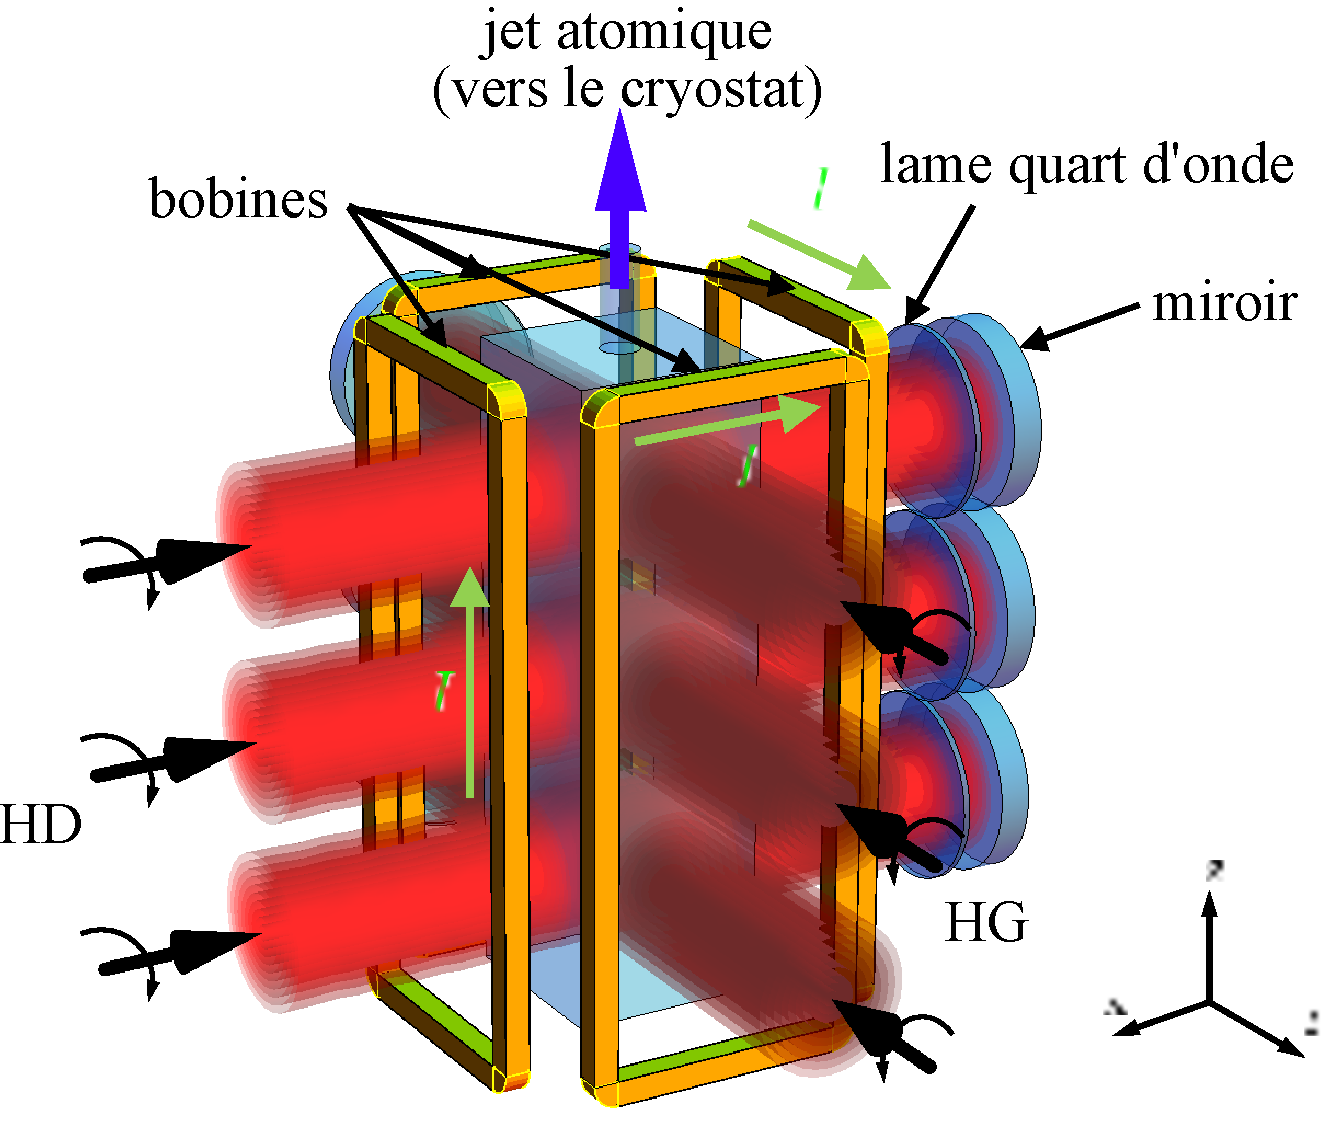
\includegraphics[width=0.6\linewidth]{figures/setup/coldatoms/2DMOT_2}
\caption[Schéma du 2D-MOT]{Schéma du 2D-MOT avec ses trois étages de piégeage.
Les polarisations des faisceaux incidents sont indiquées par les lettres HD (pour hélicité droite) et HG (hélicité gauche).%, relativement à la direction de propagation des faisceaux.
Le sens des courants dans les bobines est indiqué par les flèches vertes et la lettre $I$.
Chaque faisceau est rétro-réfléchi par un miroir, et le double passage par une lame quart d'onde permet de garantir la bonne polarisation du faisceau réfléchi.
Le jet atomique produit par le 2D-MOT est représenté par une flèche violette qui pointe vers le cryostat.
}
\label{fig:2DMOT}
\end{figure}
%

Les atomes piégés dans le 2D-MOT se propagent librement selon l'axe $z$, formant un jet vertical qui arrive jusqu'à la puce atomique à l'intérieur du cryostat.
Les atomes sont alors capturés dans un MOT de grand volume créé par les bobines de biais et le bas de la bobine \og QUAD \fg{}, représentée en figure \eqref{fig:cryo}.
Le bas de la bobine QUAD permet de créer un champ quadrupolaire similaire à celui du fil \mcal{U}, adapté au piégeage magnéto-optique.
Le nombre de spires $n=19$ de la bobine permet de multiplier par autant le courant générateur de champ dans l'équation \eqref{eq:trap_center}.
Le grand volume du champ quadrupolaire ainsi créé permet de capturer efficacement les atomes du jet.
Le chargement de ce gros \og QUAD-MOT \fg{} dure de \SIvv{1}{} à \SIvv{3}{\s}, pendant lesquels on peut y collecter quelques \SIvv{e8} atomes à une température de l'ordre de \SIvv{400}{\uK}.

Le nuage atomique est alors transféré vers un second MOT, créé cette fois par les bobines de biais et le fil \mcal{U}, comme nous l'avons mentionné en \ref{subsec:cryopuce}.
Ce \og U-MOT lointain\fg{} présente des gradients similaires au QUAD-MOT mais un volume plus petit.
Le taux de transfert entre les deux est estimé entre $\num{10}$ et $\SI{40}{\percent}$ par des observations en fluorescence du nuage.
Nous pouvons à ce moment réduire le courant dans le fil \mcal{U}, ce qui d'après les équations \eqref{eq:trap_center} et \eqref{eq:trap_center_grad} rapproche le piège de la surface de la puce et le comprime en augmentant les gradients de champ magnétique.
Les gradients de champ étant plus forts, la force de rappel de la lumière s'en trouve grandie.
On peut alors se permettre d'augmenter le désaccord des faisceaux lasers afin de refroidir le nuage atomique.
Les températures atteintes dans ce \og U-MOT proche\fg{} sont de l'ordre de $\SI{40}{\uK}$, pour un nuage d'environ $\numrange{e7}{e8}$ atomes.

%\clearpage
\subsubsection*{Les étapes intermédiaires : mélasse optique et pompage Zeeman}
\noindent L'objectif, après les étapes de piégeage magnéto-optique, est de transférer les atomes dans le piège de Ioffe-Pritchard créé par le fil \mcal{Z}.
Cela sera d'autant plus efficace que le nuage atomique sera froid, et que les atomes seront bien polarisés dans le sous-niveau Zeeman $m_F=+2$ du niveau hyperfin $\mathrm{5S1/2,F=2}$.
Avant de les transférer vers le \og piège Z \fg{}, nous faisons donc subir aux atomes deux étapes supplémentaires.

Tout d'abord, nous éteignons les champs magnétiques du U-MOT en laissant les faisceaux lasers allumés.
Cela initie une étape de mélasse optique d'une durée comprise entre $\num{1}$ et $\SI{5}{\ms}$, au cours de laquelle le désaccord laser est augmenté alors que la puissance lumineuse est graduellement diminuée jusqu'à zéro.
Cette mélasse optique nous permet de refroidir quelques $\numrange{e6}{e7}$ atomes à des températures inférieures à $\SIvv{10}{\uK}$.

Après l'extinction des lasers de mélasse, un champ magnétique de \SIrange{1}{2}{\gauss} est rapidement allumé sur la direction $-y$, qui lève la dégénérescence des sous-niveaux Zeeman.
Un laser de pompage optique polarisé $\sigma ^+$ se propageant selon $-y$ pompe alors les atomes dans le sous-niveau $m_F=+2$.
Après réflexion sur la puce ce faisceau laser repasse à travers le nuage atomique.
Son hélicité a certes été inversée par la réflexion, mais sa polarisation du point de vue des atomes est restée la même.
Les atomes sont donc encore pompés vers le sous-niveau $m_F=+2$.

%\clearpage
\subsubsection*{Le piégeage magnétique et le refroidissement évaporatif}
\noindent Lorsque le nuage atomique est bien refroidi et polarisé par les étapes de mélasse et de pompage optique, le piège magnétique est allumé.
Pour cela, un courant est imposé dans le fil \mcal{Z}.
Un champ $B_z$ est généré par les bobines, qui permet d'obtenir un champ quadrupolaire comme nous l'avons évoqué en \ref{subsec:cryopuce}, centré sur la position du nuage atomique.
Le champ au centre du piège est alors orienté selon la direction $x$ et le minimum de champ, strictement supérieur à $0$, permet d'éviter les pertes de Majorana par retournement du spin.
Un second champ de biais, $B_x$, permet en outre de limiter les pertes atomiques dues à la présence d'un bruit radio-fréquence dans notre expérience.
Ce bruit peut en effet causer des transitions atomiques vers les états non piégés $m_F<1$ et il s'agit d'ajuster $B_x$ afin d'éviter que les transitions ne soient résonantes avec la fréquence du bruit \cite{PHD_NIRRENGARTEN}.

Une fois allumé, le piège magnétique est immédiatement comprimé afin d'augmenter le taux de collision entre les atomes en vue du refroidissement évaporatif.
La compression du piège est réalisée adiabatiquement en \SI{150}{\ms}.
Le piège comprimé a des fréquences de piégeage de l'ordre de $(\omega_x,\omega_y,\omega_z) \simeq 2\pi \times (\num{24},\num{3400},\num{3400})~\si{\hertz}$ à une distance de \SI{80}{\um} de la puce.
Nous pouvons alors mettre en \oe uvre une séquence de refroidissement évaporatif radio-fréquence :
les atomes les plus chauds sont transférés vers les sous-niveaux Zeeman non piégés par des transitions radio-fréquence (RF), et ainsi sont éjectés du piège.
La fréquence de ces transitions dépend du champ magnétique vu par chaque atome, et donc de sa position dans le potentiel de piégeage.
La fréquence du signal RF, envoyé dans le fil vertical (KM) de la puce (cf figure \ref{fig:chip}), est progressivement diminuée afin d'évaporer les atomes les plus chauds en premier, puis de plus en plus froids.
Le reste du nuage thermalise vite grâce au taux de collision élevé et se trouve ainsi refroidi.
Plusieurs rampes de fréquence successives sont optimisées en durée et en puissance RF, afin d'obtenir le meilleur refroidissement du nuage atomique.
L'étape de refroidissement évaporatif dure jusqu'à \SI{5}{\second} au total.
Le schéma de principe du refroidissement évaporatif RF est donné en figure \eqref{fig:evapRF}.
%
\begin{figure}[!h]
\centering
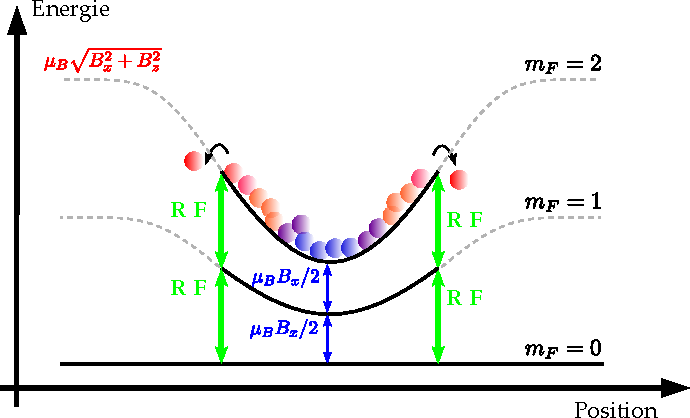
\includegraphics[width=.7\linewidth]{figures/setup/coldatoms/evapRF}
\caption[Refroidissement évaporatif RF]{Refroidissement évaporatif radio-fréquence :
le \og couteau \fg{} RF induit les transitions entre sous-niveaux Zeeman.
Une fois dans les sous-niveaux $m_F<1$, les atomes ne sont plus piégés et sont éjectés du piège.
L'aile chaude de la distribution de Boltzmann est évacuée et les atomes restant sont thermalisés à une température plus faible.
}
\label{fig:evapRF}
\end{figure}

Cette étape de refroidissement nous permet d'abaisser la température du nuage sous le seuil de condensation de Bose-Einstein.
Nous pouvons ainsi produire de façon reproductible des condensats sur puce contenant de \SIrange{10000}{20000}{} atomes.
La séquence de refroidissement peut également être interrompue avant la condensation, et en choisissant la fréquence finale de la rampe RF, nous pouvons choisir la température du nuage atomique.
La figure \eqref{fig:BEC} montre des images du nuage atomique après temps de vol pour différentes valeurs de la fréquence finale de la rampe RF.
%
\begin{figure}[!h]
\centering
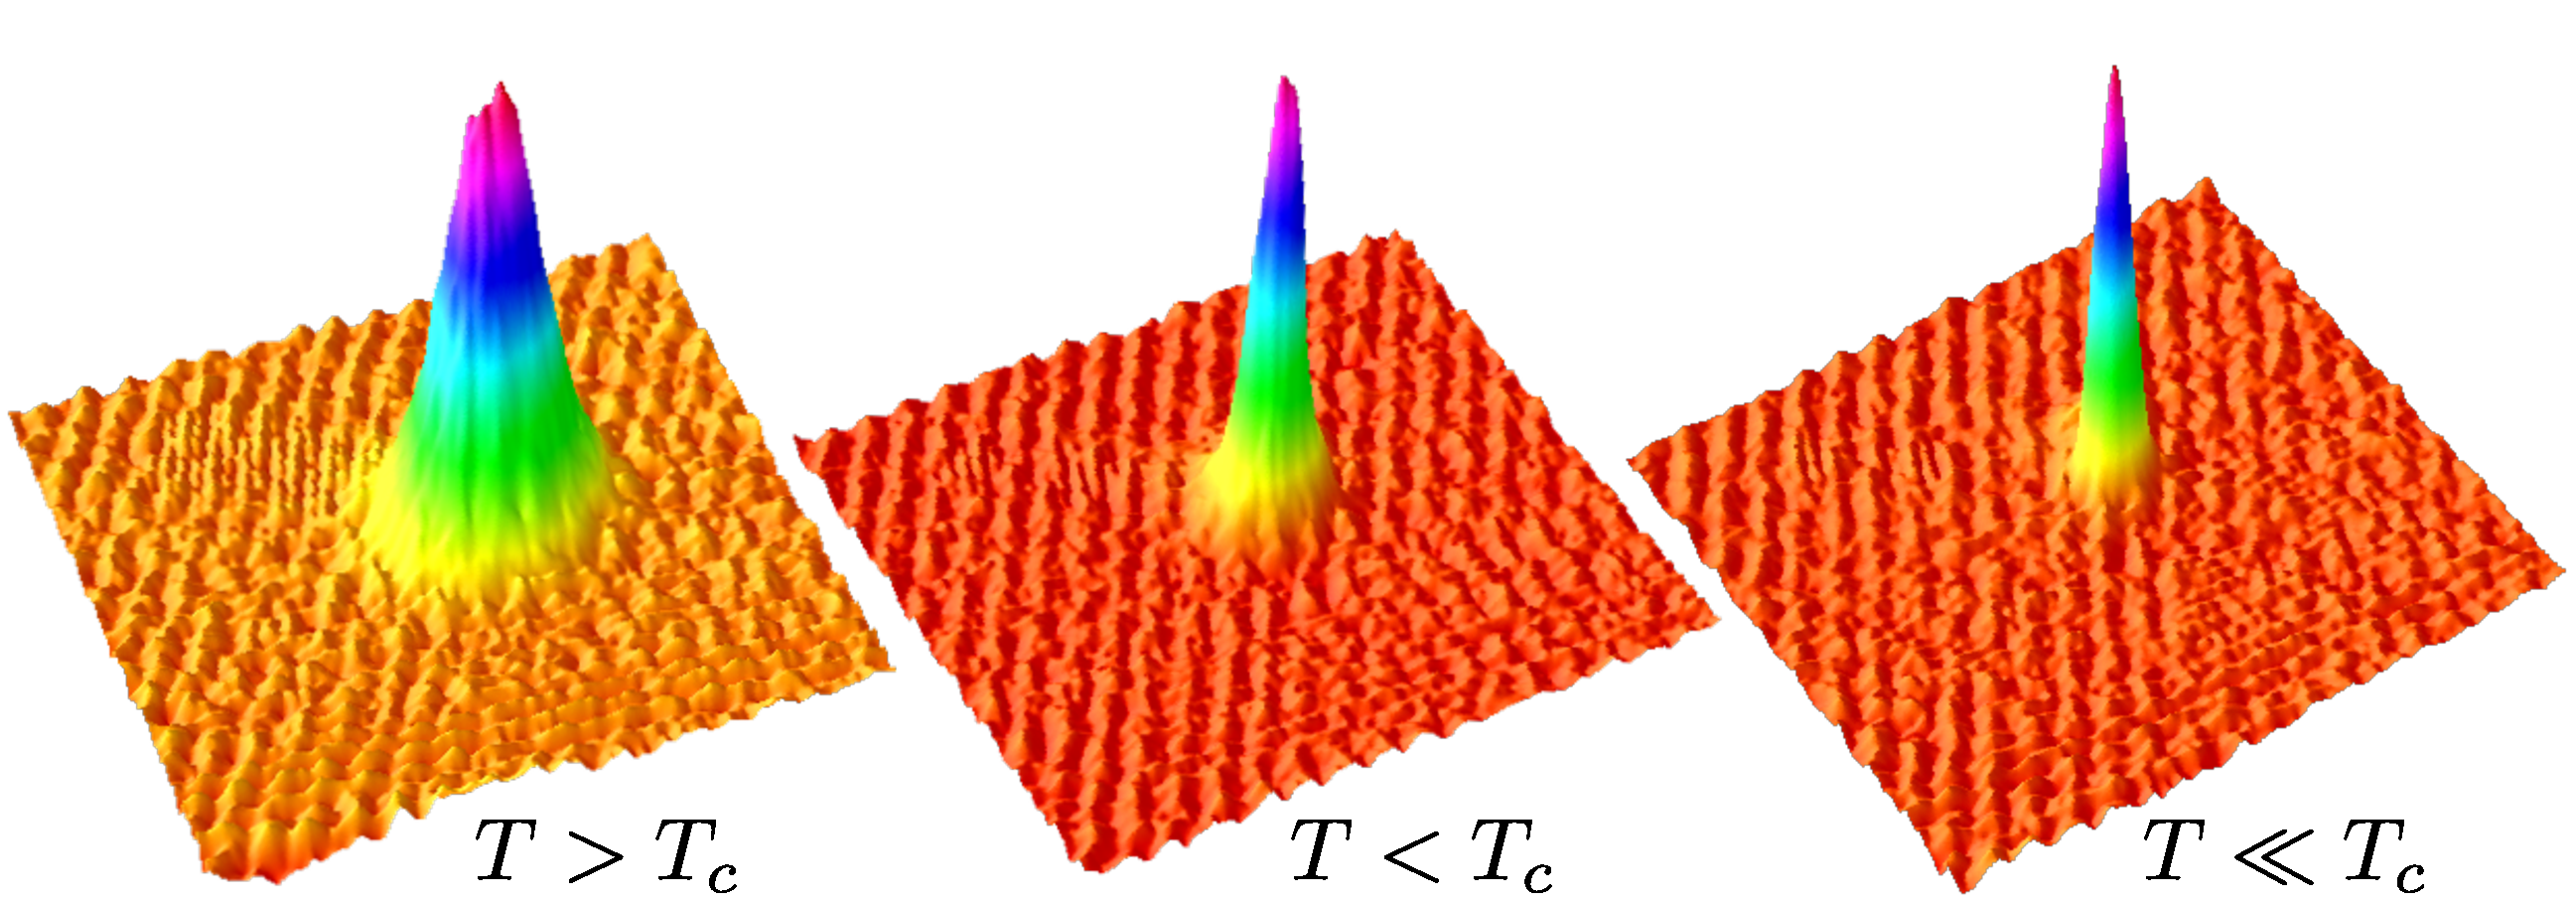
\includegraphics[width=.8\linewidth]{figures/setup/coldatoms/BEC}
\caption[Condensat de Bose-Einstein sur puce]{
Trois nuages de \Rb{87} évaporés jusqu'à des valeurs différentes de fréquence RF, imagés après un temps de vol de \SI{16.5}{\ms}.
Les images donnent directement la distribution d'impulsion au sein du nuage.
Le nuage contient environ $\SI{e4}{}$ atomes, et la tepérature critique de condensation est de l'ordre de $T_C = \SI{100}{\nano\K}$.
\`A gauche, la température est supérieure à $T_C$: le nuage est purement thermique et montre une distribution gaussienne d'impulsion.
Au milieu, la température est inférieure à $T_C$, le nuage montre un double profil en impulsion : un condensat de Bose-Einstein au centre et les atomes du nuage thermique autour.
\`A droite, la température est très petite devant $T_C$ et le condensat est quasi-pur : le nuage présente un profil de Thomas-Fermi dans l'espace des impulsions.
}
\label{fig:BEC}
\end{figure}
%

Enfin, une fois le nuage refroidi à la température souhaitée, le piège magnétique est décomprimé.
Cela permet de choisir soit une distance particulière du nuage atomique à la puce, soit la taille du nuage atomique final.

Les atomes qui seraient restés dans le sous-niveau $m_F=+1$ peuvent à leur tour être éliminés du piège en envoyant sur le nuage un signal micro-onde à \SI{6.8}{\GHz} adressant la transition hyperfine $\ket{F=2,m_F=1} \rightarrow \ket{F=1,m_F=0}$.
En présence d'un champ magnétique, les sous-niveaux Zeeman sont suffisamment résolus pour adresser uniquement cette transition, sans affecter les atomes dans le niveau $\ket{F=2,m_F=+2}$.

%\clearpage	
\subsection{Imagerie atomique par absorption}
\noindent Dans une expérience d'atomes froids, il est essentiel de pouvoir imager et dénombrer correctement le nuage atomique.
L'imagerie par absorption est une technique précise et efficace pour cela.
%Elle consiste à envoyer sur les atomes un faisceau laser, résonnant avec une transition atomique choisie, et à mesurer quelle fraction de la lumière le nuage atomique a absorbé.
Lorsqu'une telle expérience est menée au c\oe ur d'un cryostat, la tâche est rendue plus difficile en raison des accès optiques limités qui contraignent fortement l'optique d'imagerie.

\subsubsection*{Dispositif optique}
\noindent Nous pouvons imager notre nuage atomique de deux façons différentes.
Le dispositif optique d'imagerie est représenté en figure \eqref{fig:probes_CdF}.

Un premier faisceau sonde (\og sonde face \fg{})  entre dans le cryostat et en ressort perpendiculairement à la puce après réflexion sur celle-ci, par le hublot de face.
Un miroir percé permet de laisser passer le faisceau d'entrée et de collecter le faisceau de sortie, qui est ensuite envoyé vers une caméra CCD.
Grâce à l'installation d'une lentille de focale $f=\SI{100}{\mm}$ à la place du hublot de face sur la jupe hélium du cryostat, soit à environ $\SI{100}{\mm}$ de la puce, cet axe d'imagerie peut collecter beaucoup de lumière, avec une limite de résolution de $\SI{1.6}{\um}$.

Un deuxième faisceau sonde (\og sonde côté \fg{}) est envoyé par un hublot de côté ($+x$), se réfléchit sur la puce avec un angle de \SIrange{5}{10}{\degree}, et ressort par l'autre hublot de côté ($-x$). Il est ensuite envoyé vers une autre caméra CCD.
Cet axe d'imagerie ne dispose pas d'une lentille interne au cryostat. Ainsi, la lumière collectée et la résolution optique sont limitées par le diamètre du hublot de sortie du cryostat.
%le diamètre de la première lentille après la sortie du cryostat.
Cette lentille est donc placée le plus près possible de l'enceinte du cryostat.
En raison de cette géométrie, l'imagerie des atomes par la sonde côté forme deux images du nuage atomique : celui absorbe à la fois le faisceau incident et le faisceau réfléchi sur la puce.
Cela nous permet d'évaluer précisément la distance du nuage atomique à la puce : elle vaut la moitié de la distance entre les deux images du même nuage.
La figure \eqref{fig:double_cloud} montre une image d'absorption de la sonde côté par un nuage froid (piégé magnétiquement et refroidi), après un temps de vol de \SI{16.5}{\ms}.

\begin{figure}[h]
\centering
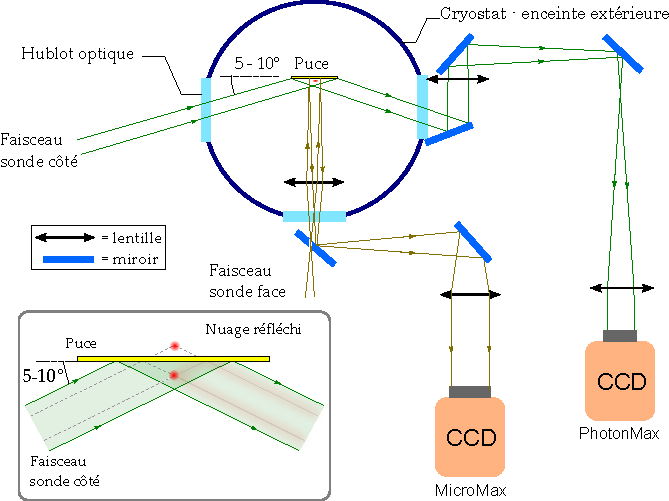
\includegraphics[width=.7\linewidth]{figures/setup/coldatoms/probes_CdF}
\caption[Faisceaux sonde]{Schéma optique des faisceaux sonde dans le cryostat.
L'insert montre de plus près la réflexion du faisceau sonde côté sur la puce et la formation des deux images du nuage.
}
\label{fig:probes_CdF}
\end{figure}

\begin{figure}[h]
\centering
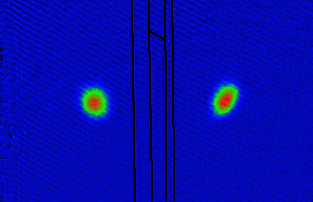
\includegraphics[width=.6\linewidth]{figures/setup/coldatoms/double_cloud_withWires}
\caption[Image par absorption du nuage par la sonde côté]{Image par absorption d'un nuage froid après temps de vol, éclairé par la sonde de côté. Les deux images du nuage sont dues à la réflexion du faisceau sur la puce.
Les ombres portées des fils de la puce sont tracées en surimpression entre les deux images du nuage.
}
\label{fig:double_cloud}
\end{figure}

%\clearpage
\subsubsection*{Principe de l'imagerie par absorption}
\noindent Les atomes peuvent être observés en temps réel par la collecte des photons qu'ils émettent par fluorescence, mais l'imagerie par absorption permet une meilleure précision sur l'estimation du nombre d'atome dans le nuage.
Elle consiste à envoyer sur les atomes un faisceau laser, résonant avec une transition atomique choisie, et à mesurer quelle fraction de la lumière le nuage atomique a absorbé.

Lorsque l'intensité lumineuse reçue par les atomes est largement inférieure à l'intensité de saturation, l'absorption de celle-ci est bien décrite par la loi de Beer-Lambert :
\begin{equation}
\label{eq:Beer-Lambert}
\frac{dI(x,y,z)}{dx} = -\sigma n(x,y,z) I(x,y,z),
\end{equation}
où $I(x,y,z)$ est l'intensité lumineuse au point de coordonnées $(x,y,z)$, $n$ la densité atomique en ce point, $x$ la direction de propagation du faisceau lumineux et $\sigma$ la section efficace de diffusion de la lumière par un atome unique.
L'optique d'imagerie nous oblige cependant à intégrer cette équation dans la direction de propagation $x$.
On obtient alors 
\begin{equation}
\label{eq:Beer-Lambert_integ}
I_f(y,z) = I_i (y,z)\cdot e^{-\int dx~\sigma~n(x,y,z)}
\end{equation}
où $I_i$ est l'intensité du faisceau incident et $I_f$ l'intensité du faisceau à la sortie du nuage atomique.

Les images enregistrées par les caméras permettent d'obtenir les quantités $I_i(y,z)$ et $I_f(y,z)$.
On peut alors calculer la densité optique du nuage , définie comme $OD(y,z) = \int dx~\sigma~n(x,y,z)$, et qui d'après l'équation \eqref{eq:Beer-Lambert_integ} est égale à
\begin{equation}
\label{eq:OD}
OD(y,z) = \int dx~\sigma~n(x,y,z) = -\ln \frac{I_f(y,z)}{I_i(y,z)}.
\end{equation}
L'on en extrait ensuite la densité atomique intégrée le long de l'axe de propagation du laser à partir de l'équation \eqref{eq:OD} :
\begin{equation}
\label{eq:atomic_density}
n(y,z) = \int{dx~n(x,y,z)} = -\frac{1}{\sigma} \ln \frac{I_f(y,z)}{I_i(y,z)} = \frac{OD(y,z)}{\sigma}.
\end{equation}
		
Dans le cas simple d'une lumière résonante avec la transition non-dégénérée d'un système à deux niveaux, la section efficace de diffusion $\sigma$ est donnée directement par la section efficace de diffusion résonante 
\begin{equation}
\sigma = \sigma_0 = \frac{3\lambda^2}{2\pi} = \frac{\Gamma \hbar\omega}{2I_{sat,0}},
\end{equation}
où $\lambda$ est la longueur d'onde de la lumière résonante et $I_{sat,0}$ l'intensité de saturation de la transition dans ce cas idéal.
Les atomes dans notre piège magnétique sont préparés dans l'état $\ket{5S1/2,F=2,m_F=+2}$, et la lumière de sonde est préparée de façon à adresser la transition $\sigma^+$ vers le niveau $\ket{5P3/2,F=3,m_F=+3}$.

\clearpage
\subsubsection*{Corrections et améliorations de l'imagerie par absorption}
\noindent Malgré l'apparente simplicité du dispositif d'imagerie par absorption, plusieurs effets perturbent les mesures du nombre d'atomes et méritent d'être corrigés.

Premièrement, la section efficace de diffusion $\sigma$ dans notre expérience n'est pas égale à la section efficace de diffusion résonante $\sigma_0$.
En effet, la lumière des faisceaux sonde n'est pas parfaitement polarisée $\sigma^+$.
De plus, les atomes ne sont pas tous dans le sous-niveau $m_F=+2$, en particulier lorsque l'on souhaite imager le nuage dans le MOT ou après l'étape de mélasse optique sans le charger dans le piège magnétique.
Enfin, l'interférence entre le faisceau sonde de côté et sa réflexion sur la puce module l'intensité de la lumière vue par le nuage atomique.
La combinaison de ces effets réduit peut être décrite en corrigeant la section efficace de diffusion d'un facteur $\alpha$ \cite{PHD_CELISTRINO,MX_GUERYODELIN_SATABSIM}.
On obtient alors une section efficace de diffusion effective $\sigma = \sigma_0 / \alpha$, ou, de façon équivalente, une intensité de saturation effective $I_{sat} = \alpha\cdot I_{sat,0}$.
La calibration expérimentale de ce paramètre $\alpha$ est effectuée par la mesure de l'intensité de saturation effective $I_{sat}$.
Pour l'absorption de la sonde de côté par un nuage dans le piège magnétique, nous obtenons une valeur $\alpha_{magn} = \num{2.06} \pm \num{0.1}$.
Pour l'absorption de la sonde de côté par un nuage juste après la mélasse optique, nous obtenons une valeur $\alpha_{melasse} = \SI{2.27}{} \pm \SI{0.1}{}$.
Le nombre d'atomes évalué à partir des images par absorption dépend directement de la valeur de ce paramètre $\alpha$.
Les valeurs expérimentales proches de $\alpha=2$ sont tout à fait cohérentes avec le fait que notre faisceau sonde est polarisé linéairement : seule la composante $\sigma^+$ de la lumière résonante avec la transition sonde peut être absorbée.
Cette composante représente la moitié de l'intensité totale envoyée, et seule cette moitié contribue à la saturation de la transition.
Pour un même paramètre de saturation, l'intensité totale du faisceau doit donc être deux fois plus grande que si le faisceau était polarisé $\sigma^+$.
	
Deuxièmement, l'acquisition du signal d'imagerie se fait en trois temps.
Une première image est enregistrée où les atomes absorbent le faisceau sonde, ce qui nous donne l'intensité $I_f$.
Puis une deuxième image est enregistrée après que les atomes sont tombés par gravité, qui nous donne l'intensité du faisceau sonde non absorbé $I_i$.
Enfin, une troisième image est enregistrée sans aucun laser allumé, qui permet de soustraire la lumière de fond
%et le bruit électronique
des deux images précédentes.
Les délais de quelques dizaines de \si{\ms} entre les différentes images ont un effet délétère sur le signal.
En effet, le signal enregistré par la caméra subit un bruit d'imagerie sous la forme de franges, dues à la diffraction et aux interférences du faisceau laser le long de son chemin optique et lors de sa réflexion sur la surface de la puce.
Des vibrations et déformations de petite amplitude des éléments optiques et des variations d'indice de l'air le long du chemin optique décalent ces franges d'une image à l'autre.
L'opération de traitement des images (équation \ref{eq:atomic_density}) ne permet pas de d'affranchir des fluctuations de ces franges, qui viennent ainsi brouiller le signal d'imagerie.
%génèrent des franges dans les images traitées par l'équation \eqref{eq:atomic_density}, semblables à des franges d'interférence.
Ce problème se présente principalement sur l'imagerie par la sonde de face en raison des plus grands délais exigés par la caméra et de la plus grande sensibilité mécanique du chemin optique.
Afin d'y remédier, nous avons implémenté un algorithme de réduction des franges qui, à partir d'une base de plusieurs images du faisceau sonde seul, reconstitue la meilleure combinaison linéaire de celles-ci pour chaque image où le nuage atomique est présent. Cet algorithme est décrit en détail dans \cite{MX_WHITLOCK_FRINGEREDUCTION}.
La figure \eqref{fig:Fringe_Reduction} montre une image d'un nuage froid par absorption de la sonde face, non traitée et après traitement par cet algorithme.

\begin{figure}[h]
\centering
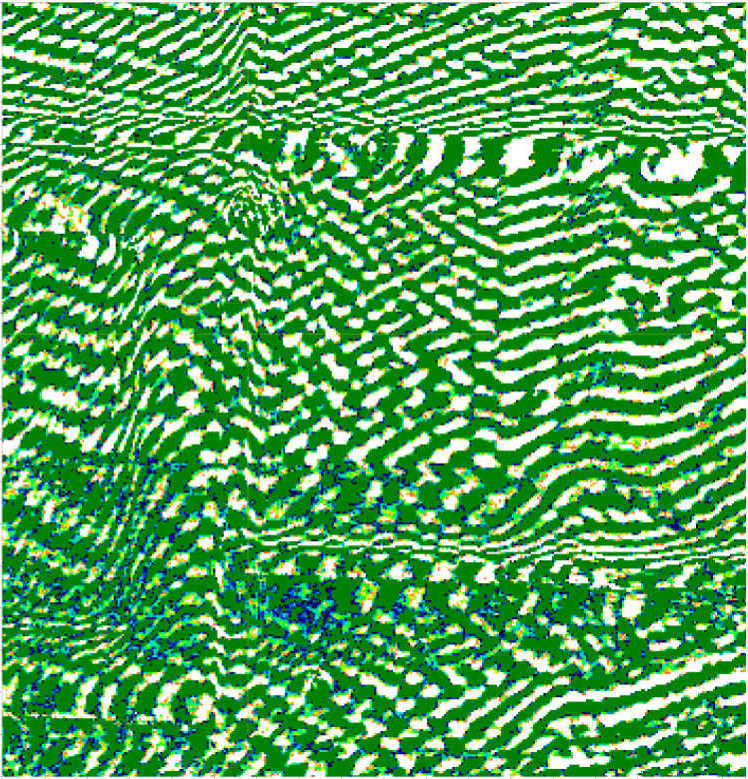
\includegraphics[width=0.35\linewidth]{figures/setup/coldatoms/Normal_abs2_onlyPic}
\hspace{.15\linewidth}
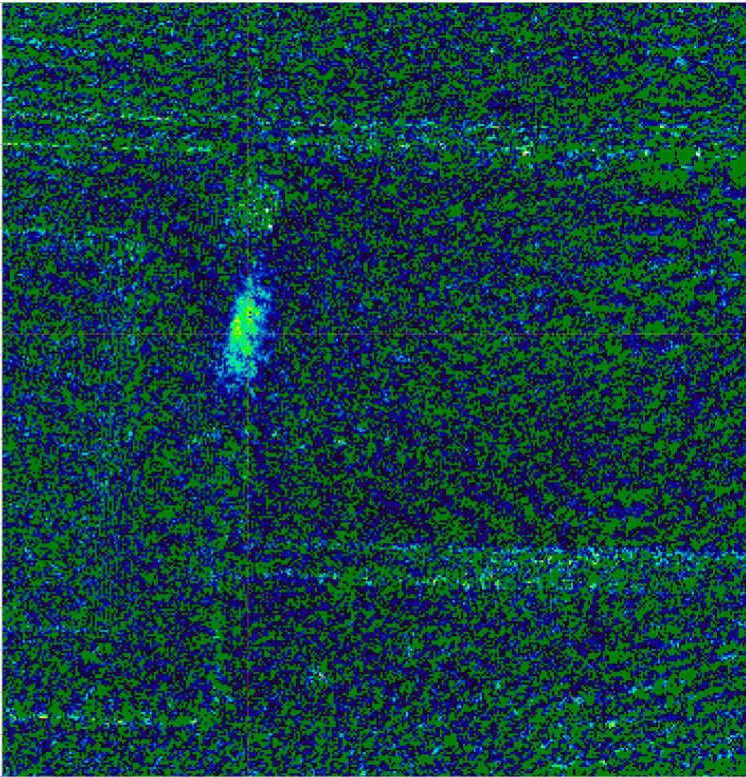
\includegraphics[width=0.35\linewidth]{figures/setup/coldatoms/RF_abs2_onlyPic}
\caption[Effet de l'algorithme de réduction des franges]{
Images du nuage atomique froid par absorption du faisceau sonde face.
\`A gauche, l'image est traitée selon l'équation \eqref{eq:atomic_density}.
\`A droite, la même image après traitement par l'algorithme de réduction des franges.
Les graphes sous les images sont les profils de densité du nuage en coupe horizontale.
L'échelle de couleur est la même pour les deux images et a été optimisée pour l'image de droite.
}
\label{fig:Fringe_Reduction}
\end{figure}

\newpage
Troisièmement, %il peut être intéressant, pour caractériser des nuages très denses, de ne pas calculer la densité optique $OD$ comme à l'équation \eqref{eq:Beer-Lambert_integ}.
%En effet, 
dans le cas d'un nuage très dense optiquement, comme par exemple pour les mélasses optiques, le centre du nuage où la densité atomique est très haute peut absorber l'intégralité de l'intensité incidente $I_i$.
Le rapport des intensités $I_f/I_i$ est alors très faible et dominé par le bruit.
Le signal $I_f/I_i$ au centre du nuage peut ainsi présenter des valeurs négatives, qui seront problématiques lorsque l'on souhaitera en prendre le logarithme.
%Or la valeur de la densité optique au centre du nuage est cruciale à l'ajustement de la densité à un profil gaussien.
Afin de remédier à cela, il peut être intéressant de ne pas calculer la densité optique $OD$ comme à l'équation \eqref{eq:Beer-Lambert_integ}, mais de s'arrêter à l'opération 
\begin{equation}
\label{eq:nolog_abs}
\frac{I_f(y,z)}{I_i(y,z)} = e^{-OD(x,y)} = e^{-\sigma .n(y,z)}.
\end{equation}
Nous appellerons cette opération \og absorption no-log \fg{}.
%Si le nuage présente un profil de densité gaussien, cela permet de se concentrer sur les ailes de ce profil.
Ce traitement du signal permet de s'affranchir de \og l'amplification \fg{} du bruit au centre par le logarithme et du problème des valeurs négatives, en se concentrant sur le signal aux bords du nuage.
Le profil de densité est alors ajusté à l'exponentielle d'un profil gaussien.
%L'ajustement du profil de densité est alors meilleur sur les bords du nuages.
La figure \eqref{fig:nolog_abs} montre l'image d'une mélasse optique par absorption de la sonde de côté, traitée d'après l'équation \eqref{eq:Beer-Lambert_integ} et d'après l'équation \eqref{eq:nolog_abs}.
		

\begin{figure}[h]
\centering
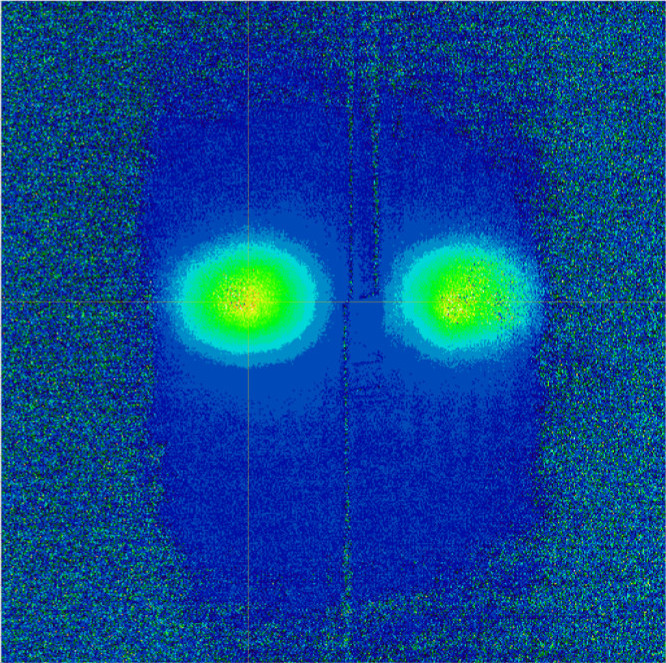
\includegraphics[width=0.35\linewidth]{figures/setup/coldatoms/log_abs_onlyPic}
\hspace{.15\linewidth}
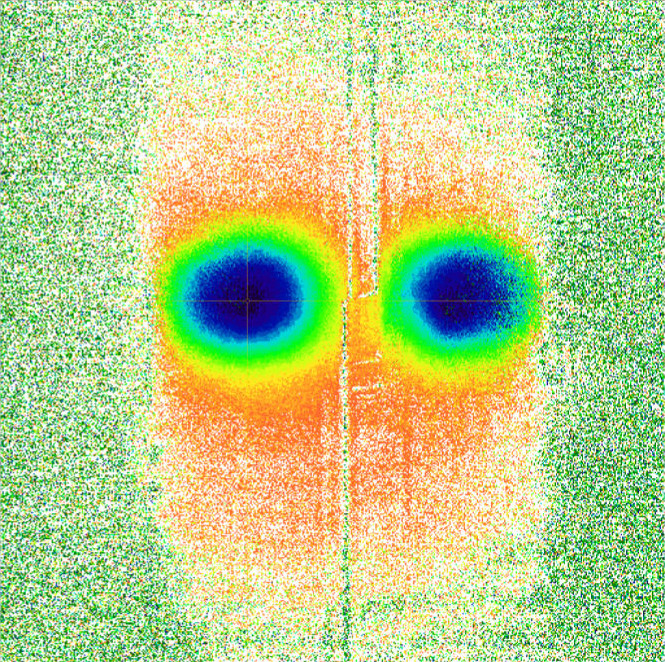
\includegraphics[width=0.35\linewidth]{figures/setup/coldatoms/nolog_abs_onlyPic}
\caption[Absorption \og no-log \fg{} ]{
Images du nuage atomique de mélasse optique par absorption du faisceau sonde côté.
\`A gauche, l'image est traitée par absorption selon l'équation \eqref{eq:Beer-Lambert_integ}.
\`A droite, l'image est traitée selon l'équation \eqref{eq:nolog_abs}.
Les graphes sous les images sont les profils de densité du nuage en coupe horizontale.
L'échelle de couleur est différente pour les deux images, adaptée à l'échelle des profils en coupe représentés.
Les zones bruitées à gauche et à droite ne sont pas éclairées par le faisceau sonde. 
En absorption \og no-log \fg{}, le bruit est plus important dans les zones sombres, mais réduit au centre et sur les bords du nuage.
%Le bruit y est beaucoup plus important si l'on ne prend pas le logarithme du signal (image de droite).
%Cependant, le bruit y est fortement réduit au centre du nuage.
}
\label{fig:nolog_abs}
\end{figure}	

%\clearpage
\subsubsection*{Estimation de la température}
\noindent L'imagerie par absorption permet facilement d'estimer la température du nuage atomique.
En effet, la distribution des impulsions dans le nuage suit la distribution de Maxwell-Boltzmann tant que celui-ci n'est pas condensé.
L'évolution de la taille gaussienne du nuage après extinction du piège, dictée par l'impulsion moyenne dans le nuage,  nous renseigne alors sur sa température par l'équation de propagation balistique
\begin{equation}
\label{eq:tempfit}
\Delta x^2 (t) = \Delta x^2(t_0) + \frac{\kb T}{m} \cdot (t-t_0)^2,
\end{equation}
où $\Delta x$ est l'extension spatiale du nuage dans la direction $x$, $t$ le temps et $t_0$ la référence de temps, $\kb$ la constante de Boltzmann, $m$ la masse d'un atome et $T$ la température du nuage.
En imageant le nuage à différents moments de son expansion (\og temps de vol \fg{}) et en ajustant la largeur gaussienne du profil à l'équation \eqref{eq:tempfit}, on accède à la fois à la température $T$ du nuage et à sa taille initiale dans le piège $\Delta x(t=0)$.
La figure \ref{fig:Tempfit} représente un ajustement de l'évolution de la taille du nuage après relâchement du piège.
%
\begin{figure}[!h]
\centering
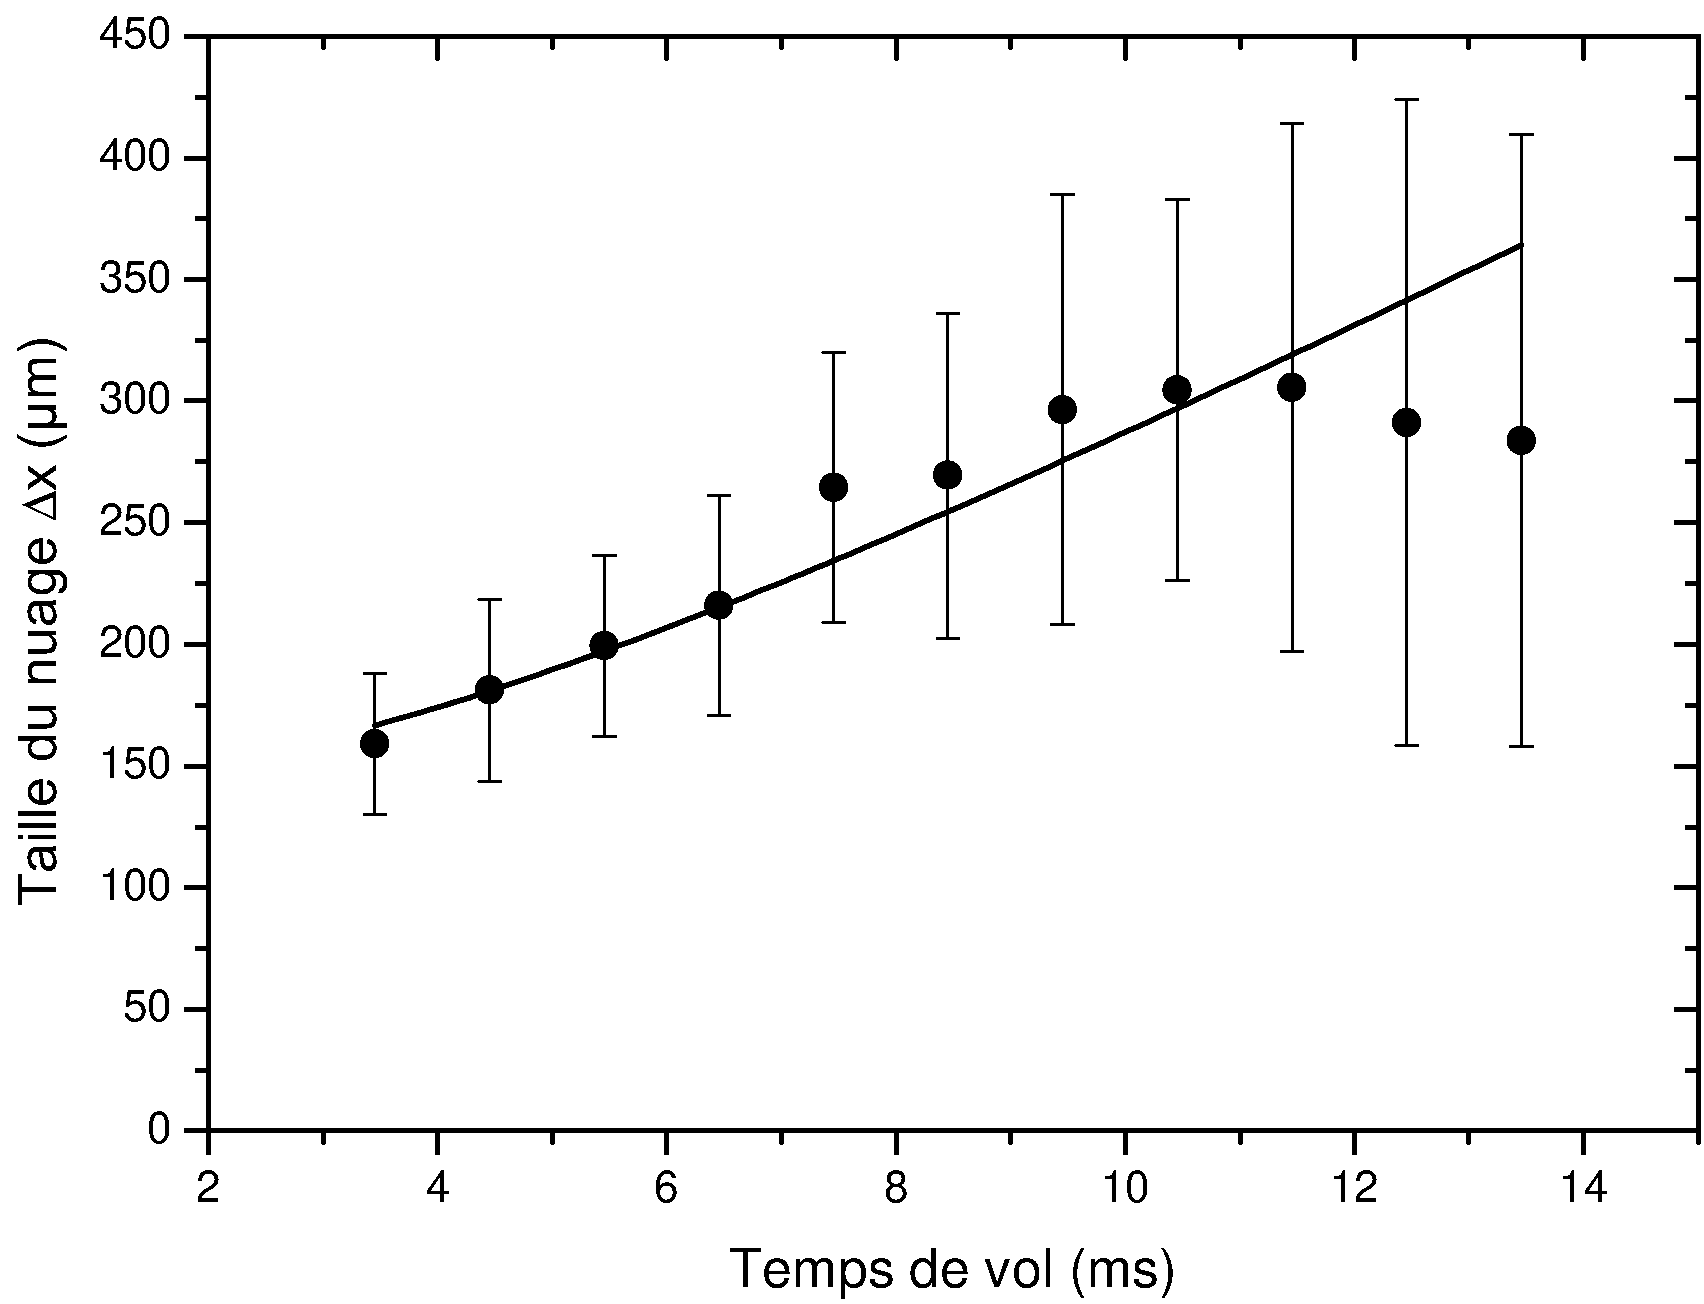
\includegraphics[width=.6\linewidth]{figures/setup/coldatoms/Tempfit}
%donnees du 1er sept 2017
\caption[Estimation de la température d'un nuage par temps de vol]{
Estimation de la température d'un nuage par temps de vol.
Le graphe représente l'évolution de la taille d'un nuage de mélasse optique, en fonction du temps écoulé depuis l'extinction des lasers.
L'ajustement selon l'équation \eqref{eq:tempfit} permet d'estimer la température du nuage à $\SI{6.43}{} \pm\SI{1}{\uK}$, et sa taille initiale à $\SI{142}{} \pm \SI{13}{\um}$.
}
\label{fig:Tempfit}
\end{figure}
	
\clearpage	
\subsection{Quelques nuages typiques}
\noindent Nous avons décrit ici les éléments de notre dispositif qui servent à produire et caractériser des nuages d'atomes ultra-froids.
Le tableau \ref{tab:nuages} présente les caractéristiques principales des différents types de nuages atomiques que nous utiliserons pour y exciter des atomes de Rydberg.

\begin{table}[h!]
	\centering
	\caption[Quelques nuages typiques]{Quelques nuages typiques de notre expérience.
	Pour chacun, nous donnons les caractéristiques suivantes : nombre d'atomes $N$, taille $\Delta x$ du nuage selon $x$, taille $\Delta y,z$ du nuage selon $y$ et $z$, température $T$ est distance à la puce $d$.
	}
	\label{tab:nuages}
	\begin{tabular}{c | c c c c c}
		\toprule\midrule
		{nuage}
		&N 
		&$\Delta x$
		&$\Delta y,z$
		&T
		&d
		\\
		\midrule
		QUAD-MOT
		&quelques \num{e8}
		&
		&
		&\SI{400}{\uK}
		&\SIrange{1}{3}{\mm}
		\\
%		U-MOT lointain
%		&
%		&
%		&
%		&idem
%		&idem
%		\\
		U-MOT proche
		&\SI{e7}
		&\SI{200}{\um}
		&\SI{200}{\um}
		&\SI{40}{\uK}
		&\SI{600}{\um}
		\\
		mélasse optique
		&\SI{5e6}
		&\SI{80}{\um}
		&\SI{80}{\um}
		&\SI{10}{\uK}
		&\SI{600}{\um}
		\\
		piège mag. chaud
		&\SI{1.5e6}
		&
		&
		&\SI{40}{\uK}
		&
		\\
		piège mag. froid
		&\SI{1.2e4}
		&\SI{45}{\um}
		&\SI{4.5}{\um}
		&\SI{0.75}{\uK}
		&\SI{450}{\um}
		\\
		BEC
		&\SIrange{8000}{20000}
		&
		&
		&\SIrange{30}{80}{\nano\K}
		&
		\\
		\midrule
		\bottomrule
 	\end{tabular}
\end{table}

\noindent Ces différents nuages d'atomes froids, ou ultra-froids, vont nous permettre d'explorer l'excitation d'atomes de Rydberg dans différentes conditions.

\clearpage
\section{Excitation et détection d'atomes de Rydberg près d'une puce}

\noindent Cette diversité de nuages atomiques nous permet d'exciter des atomes de Rydberg dans différentes conditions de densité atomique, de température et de distance à la puce.
Nous présentons dans le reste de ce chapitre la partie de notre dispositif expérimental servant à exciter, détecter et manipuler les atomes de Rydberg.
Notre dispositif est particulier dans la mesure où tout ce qui concerne les niveaux de Rydberg a lieu près d'une surface, la puce atomique.
Des champs parasites électriques parasites étant inévitables à proximité d'une surface, la grande sensibilité électromagnétique des atomes de Rydberg sera mise à rude épreuve.

Après avoir donné le principe de l'excitation à deux photons des niveaux de Rydberg et de la détection par ionisation sélective, nous ferons une présentation de rapide de l'effet Stark et de ses conséquences sur nos expériences.
Nous décrirons ensuite les techniques mises en place afin de contrôler les champs électriques près de la puce.
Nous finirons ce chapitre par une présentation de la technique de spectroscopie microonde des niveaux de Rydberg et de son utilisation pour mesurer les champs électriques résiduels.

%\clearpage
\subsection{L'excitation à deux photons des atomes de Rydberg}\label{subsec:2photon_excite}
\noindent Les atomes de rubidium piégés dans un nuage près de la puce sont excités vers les niveaux de Rydberg par une transition laser à deux photons désaccordée par rapport au niveau intermédiaire.
Dans nos expériences, deux niveaux de Rydberg différents ont été excités par laser à partir de l'état fondamental 5S$_{1/2}$ : le niveau 60S$_{1/2}$ et le niveau 50D$_{3/2}$.
Nous décrivons ici l'excitation d'un nuage d'atomes de Rydberg au sein d'un nuage froid dans le piège magnétique, en négligeant les interactions entre atomes de Rydberg et en nous concentrant sur le niveau $\mathrm{60S_{1/2}}$.

La transition du niveau fondamental au niveau de Rydberg est faite par l'absorption d'un photon rouge à $\lambda = \SI{780}{\nano\meter}$, désaccordé de $\delta=+2\pi\times\SI{540}{\MHz}$ par rapport à la transition $\mathrm{5S_{1/2},F=2 \rightarrow 5P_{3/2},F'=3}$, et d'un photon bleu à $\lambda = \SI{480}{\nano\meter}$, accordé pour satisfaire la condition de résonance vers le niveau choisi.
La figure \eqref{fig:2photons} représente le schéma de niveaux de l'excitation du niveau $\mathrm{60S_{1/2}}$.
Les deux faisceaux d'excitation sont superposés et se propagent selon la direction $+x$. Leurs polarisations sont définies par rapport à l'axe de quantification des niveaux atomiques, déterminé par le champ magnétique de biais $B_x$ dans le fond du piège.
La figure \eqref{fig:lasers_excit} représente la géométrie des faisceaux laser d'excitation.
Dans cette configuration, seul le sous-niveau $m_j=+1/2$ du niveau 60S est excité.
%
\begin{figure}[!h]
\centering
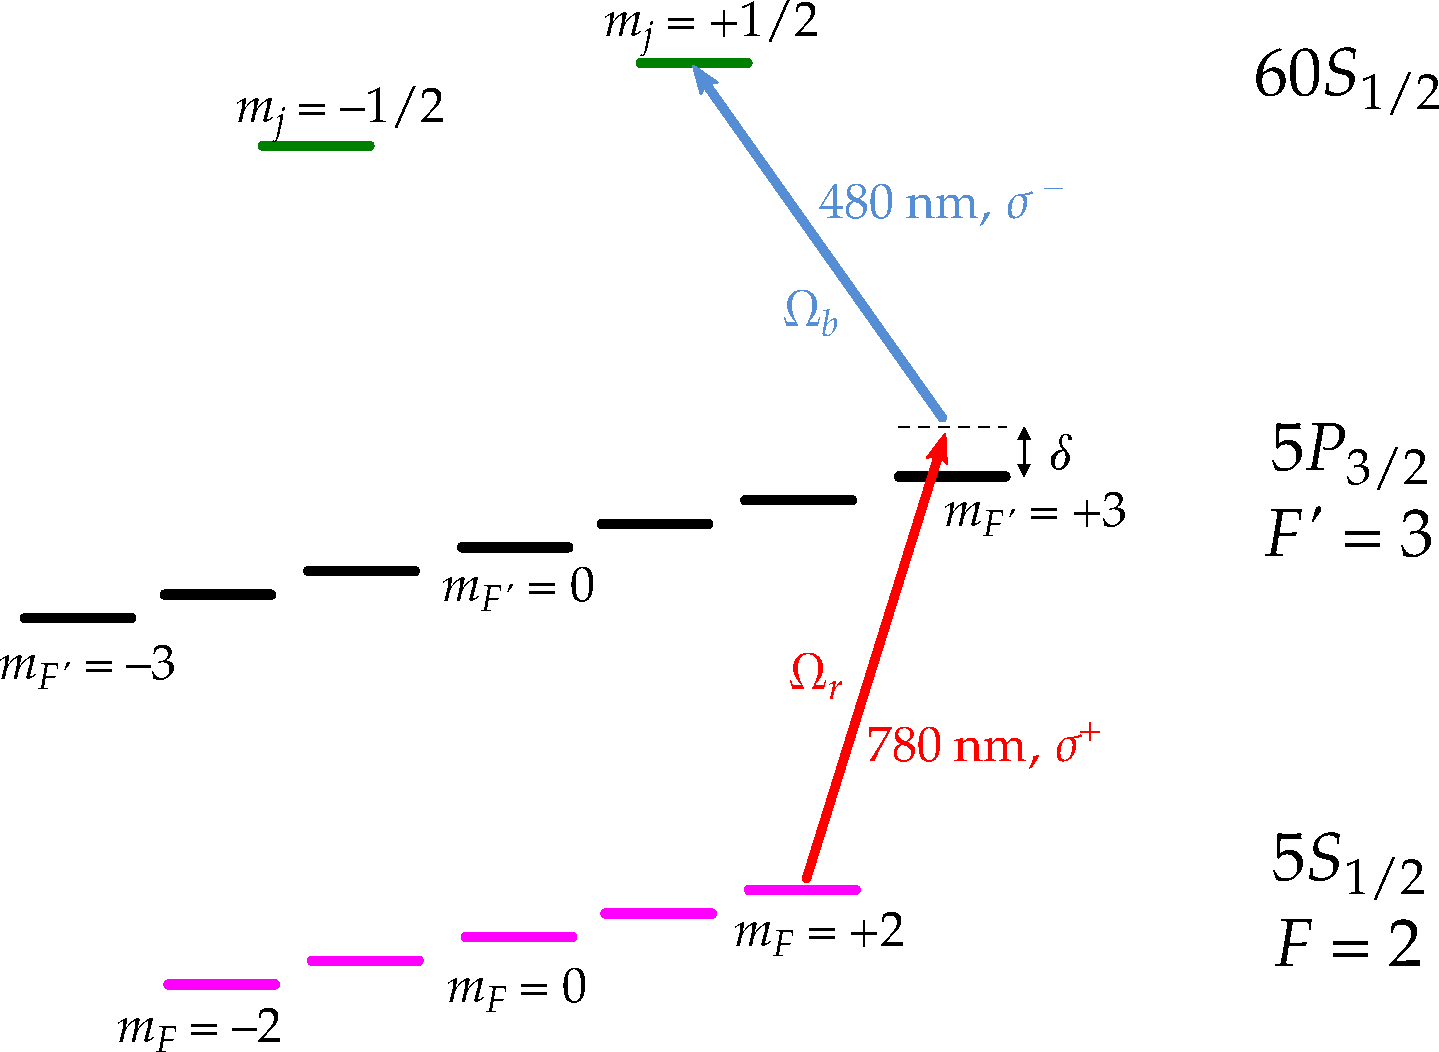
\includegraphics[width=.7\linewidth]{figures/setup/rydberg/2photons}
\caption[Excitation du niveau 60S]{Schéma de l'excitation laser du niveau 60S, à partir d'atomes de \Rb{87} dans le niveau fondamental dans le piège magnétique.
La polarisation de chaque laser est indiquée.
$\Omega_r$ et $\Omega_b$ sont les fréquences de Rabi des transitions à \num{780} et \SI{480}{\nano\meter} respectivement.
$\delta=+2\pi\times\SI{540}{\MHz}$ est le désaccord par rapport au niveau intermédiaire.
}
\label{fig:2photons}
\end{figure}

Le laser rouge d'excitation est extrait du laser maître, mentionné en \ref{subsec:exp_seq}, puis décalé en fréquence par un modulateur acousto-optique.
Le laser bleu à $\SI{480}{\nm}$ est généré par un système commercial TOPTICA TA-SHG 110 de diode laser amplifiée puis doublée en fréquence.
La lumière laser à $\SI{960}{\nm}$ est asservie en fréquence à la même cavité de Fabry-Pérot que le laser maître.
Un modulateur acousto-optique intervient entre la diode et la cavité Fabry-Pérot, qui nous permet de contrôler la fréquence de la diode sur une plage d'environ $\SI{75}{\MHz}$.
%Le laser à $\SI{960}{\nm}$ est ensuite amplifié puis doublé en fréquence grâce à un cristal non-linéaire placé dans une cavité.
Après doublage de la fréquence, cela correspond à un balayage de la fréquence du laser bleu sur une plage de $\SI{150}{\MHz}$.
Le système de stabilisation et de distribution des faisceaux laser d'excitation des niveaux de Rydberg est détaillé en annexe \ref{app:laserlock}.

Le faisceau rouge a typiquement un col de $\SI{150}{\um}$ et une puissance de $\SI{50}{\micro\watt}$ au niveau des atomes.
Le laser rouge est désaccordé de $\delta=+\SI{540}{\MHz}$ par rapport à la transition $ \ket{\mathrm{5S_{1/2},F=2,m_F=+2}} \rightarrow \ket{\mathrm{5P_{3/2},F'=3,m_F'=+3}}$, dont le moment de transition dipolaire vaut $\SI{2.98931 (62)} ea_0$ \cite{DATA_STECKRB87}.
D'après les caractéristiques du faisceau, la fréquence de Rabi correspondant à cette transition est de l'ordre de $\Omega_r \simeq 2\pi\times \SI{40}{\MHz}$.
Le taux d'émission spontanée de photons rouge par le niveau intermédiaire, de durée de vie $\Gamma^{-1} \simeq \SI{26}{\ns}$, est donné par
\begin{equation}
\label{eq:scattering_5P3/2}
\Gamma_{sp} = \frac{1}{2} \frac{\Omega_r^2 \Gamma}{\delta^2 + \Omega_r^2 + \Gamma^2}
\simeq \frac{\Omega_r^2}{2\delta^2} \Gamma,
\end{equation}
où $\Gamma = 2\pi \times \SI{6.065}{\MHz}$ est la largeur naturelle du niveau $\mathrm{5P_{3/2}}$.
La dernière égalité est vérifiée dans l'approximation $\delta^2 \gg \Omega_r^2, \Gamma^2$, qui est ici valide.
Avec nos valeurs d'intensité et de désaccord du laser, on obtient $\Gamma_{sp} \simeq \num{2.74e-3} \Gamma = 2\pi\times \SI{0.0166}{\MHz}$, ce qui correspond à l'émission d'un photon  toutes les $\Gamma_{sp}^{-1} = \SI{9.565}{\us}$.
Or lorsqu'un atome absorbe et ré-émet un tel photon, il gagne une énergie moyenne
$\Delta E = p^2/(2m_{Rb87}) = h^2/(2m_{Rb87} \lambda^2) = \frac{3}{2}\kb\times\SI{120}{\nano\kelvin}$.
Étant données nos valeurs d'intensité et de désaccord, cela implique un taux de chauffage de $\Gamma_{sp}\,\Delta E /\kb = \SI{12.6}{\nano\K/\us}$.
Le piège est ainsi chauffé par le laser rouge d'excitation, %\footnote{
%Le problème du chauffage du nuage est discuté plus en détail en \ref{subsec:rate_equation}.}
ce qui limite à la fois la puissance que l'on peut envoyer sur le nuage, et le nombre d'impulsions laser d'excitation que l'on peut faire subir à un même nuage sans l'altérer.

Le faisceau bleu a typiquement un col de $\SI{22}{\um}$ et une puissance estimée à $\SI{4}{\milli\watt}$ au niveau des atomes.
Le moment dipolaire de la transition $ \ket{\mathrm{5P_{3/2},F'=3,m_F'=+3}} \rightarrow \ket{\mathrm{60S_{1/2},m_j=+1/2}}$ est cependant bien plus faible que le précédent, et vaut $\SI{9.9e-3} ea_0$
\footnote{Nous rappelons ici que, comme nous l'avons mentionné en \ref{sec:alkalRydberg}, le bon nombre quantique magnétique pour les niveaux de Rydberg est $m_j$ et non pas $m_F$.}.
La fréquence de Rabi pour cette transition est alors de $\Omega_b = 2\pi\times \SI{8}{\MHz}$.
Les fréquences de Rabi des deux transitions satisfont l'approximation $\Omega_{r,b} \ll \delta$, ce qui nous permet de négliger l'occupation du niveau intermédiaire, et donc de l'éliminer adiabatiquement \cite{TXT_ASPECTFABRE_QUANTOPT}.
Le système à trois niveaux se ramène alors à un système effectif à deux niveaux, couplés par une fréquence de Rabi
\begin{equation}
\label{eq:Rabi_2photons}
\Omega = \frac{\Omega_r \Omega_b}{\delta}.
\end{equation}
Avec nos paramètres, on obtient une fréquence de Rabi $\Omega = 2\pi \times \SI{296}{\kHz}$ pour la transition $\ket{\mathrm{5S_{1/2},F=2,m_F=+2}} \rightarrow \ket{\mathrm{60S_{1/2},m_j=+1/2}}$.
Ce paramètre peut être varié simplement en ajustant la puissance du laser rouge ou la puissance du laser bleu.

%
\begin{figure}[!h]
\centering
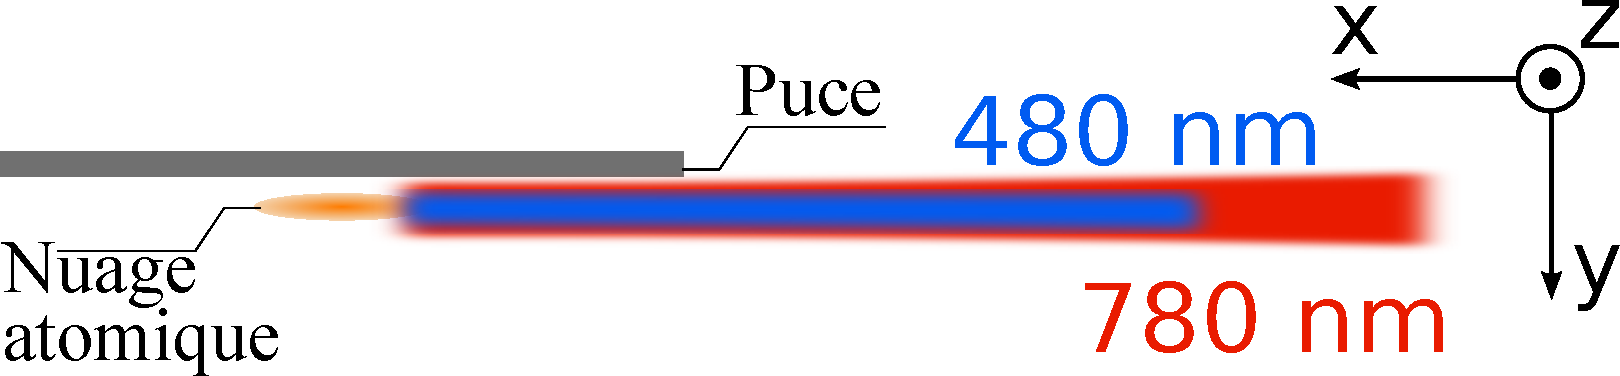
\includegraphics[width=.6\linewidth]{figures/setup/rydberg/lasers_excit}
\caption[Faisceaux laser pour l'excitation des Rydberg]{Schéma représentant la géométrie des faisceaux laser d'excitation.
}
\label{fig:lasers_excit}
\end{figure}

%\clearpage	
\subsection{La détection par ionisation des atomes de Rydberg}\label{subsec:detection}
\noindent L'électron de valence d'un atome de Rydberg alcalin est très proche du seuil d'ionisation.
Il est donc très facile de l'arracher au noyau en appliquant un champ électrique.
Nous exploitons cette caractéristique pour détecter les atomes de Rydberg par ionisation en champ électrique :
une fois l'atome ionisé, le c\oe ur atomique est accéléré par des électrodes vers un détecteur à avalanche (Channeltron).


%
\begin{figure}[h]
\centering
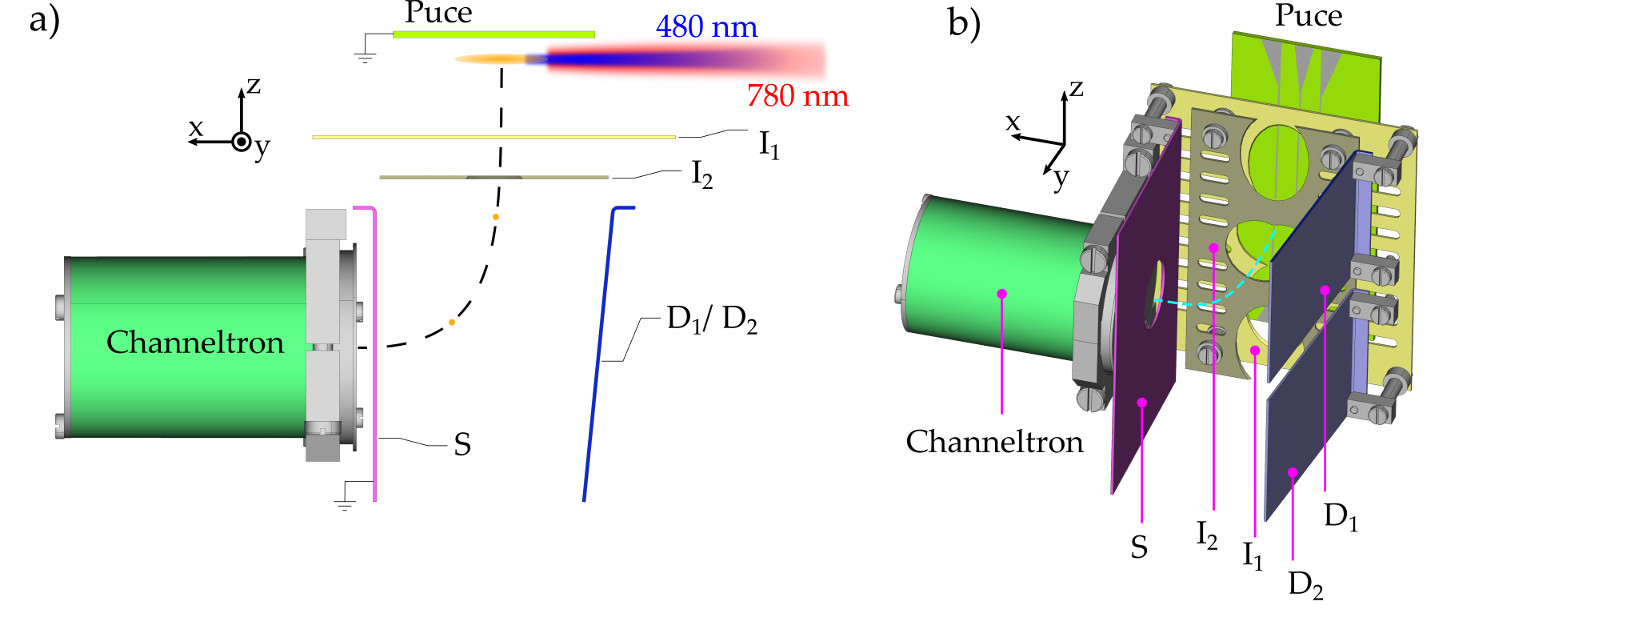
\includegraphics[width=\linewidth]{figures/setup/rydberg/schema_detect}
\caption[Système de détection des atomes de Rydberg]{Schéma représentant le système de détection des atomes de Rydberg.
\textbf{a)} vu de dessus et \textbf{b)} en projection axonométrique.
Après excitation, les atomes de Rydberg sont ionisés par les élctrodes $I_1$ et $I_2$.
Les ions ainsi créés et accélérés sont défléchis par les électrodes $D_1$ et $D_2$, en direction du détecteur Channeltron.
L'électrode $S$ est mise à la masse et sert à écranter la tension présente à l'entrée du Channeltron.
La trajectoire des ions est indiquée en lignes pointillées et les faisceaux lasers d'excitation sont représentés en \textbf{a)}.
}
\label{fig:schema_detect}
\end{figure}
%
La figure \eqref{fig:schema_detect} présente un schéma détaillé du système de détection par ionisation.
Au moment de la détection, une tension négative est appliquée sur les électrodes d'ionisation $I_1$ et $I_2$.
La tension sur ces électrodes crée un champ électrique de l'ordre de quelques $\SI{100}{\V/\cm}$ au niveau des atomes, la puce étant mise à la masse.
Ce champ électrique ionise les atomes de Rydberg et accélère les ions positifs ainsi créés.
Ces ions sont ensuite défléchis en direction du Channeltron par les électrodes $D_1$ et $D_2$, mises en permanence à un potentiel $V_{defl} = +\SI{150}{\V}$.
Une grille placée à l'entrée du Channeltron est alimentée par une tension de $\SI{-3000}{\V}$.
Une électrode trouée mise à la masse est placée devant cette grille afin d'écranter les $\SI{-3000}{\V}$ pour la région de piégeage des atomes.
Lorsque les ions arrivent dans le Channeltron, celui-ci génère par avalanche un signal électronique qui est envoyé vers un amplificateur et un discriminateur permettant de décompter les ions détectés.
Le Channeltron est isolé thermiquement et chauffé à une température de $\SI{42}{\K}$ afin d'augmenter son efficacité.

\newpage
\subsubsection*{Sélectivité de niveau de la détection par ionisation}
\noindent Chaque atome de Rydberg présente une énergie différente, telle que discutée en \ref{sec:alkalRydberg}.
Cela signifie qu'ils sont tous à une distance différente du seuil d'ionisation, et \textit{in fine} que chaque niveau de Rydberg sera ionisé pour une valeur de champ électrique spécifique.
On peut ainsi appliquer une rampe de tension sur les électrodes d'ionisation, afin que chaque niveau de Rydberg soit ionisé à un instant différent.
Alors, les ions correspondants seront détectés à des instants différents par le Channeltron et pourront être distingués.
Des fenêtres temporelles de détection peuvent alors être définies, qui permettent de compter les atomes détectés dans chacun des différents niveaux.
La figure \eqref{fig:arrTimes6057} montre un signal de détection sélective des niveaux de Rydberg $\mathrm{60S_{1/2}}$ et $\mathrm{57S_{1/2}}$.
La rampe de tension et les fenêtres temporelles de détection sont optimisées afin de distinguer au mieux les différents niveaux de Rydberg détectés.
L'efficacité de détection de notre dispositif a été mesurée à $\SI{90}{} \pm \SI{10}{\percent}$, en comparant le nombre d'atomes de Rydberg détectés par ionisation à la réduction du nombre d'atomes dans l'état fondamental mesuré par absorption \cite{PHD_CELISTRINO}.
%
\begin{figure}[!h]
\centering
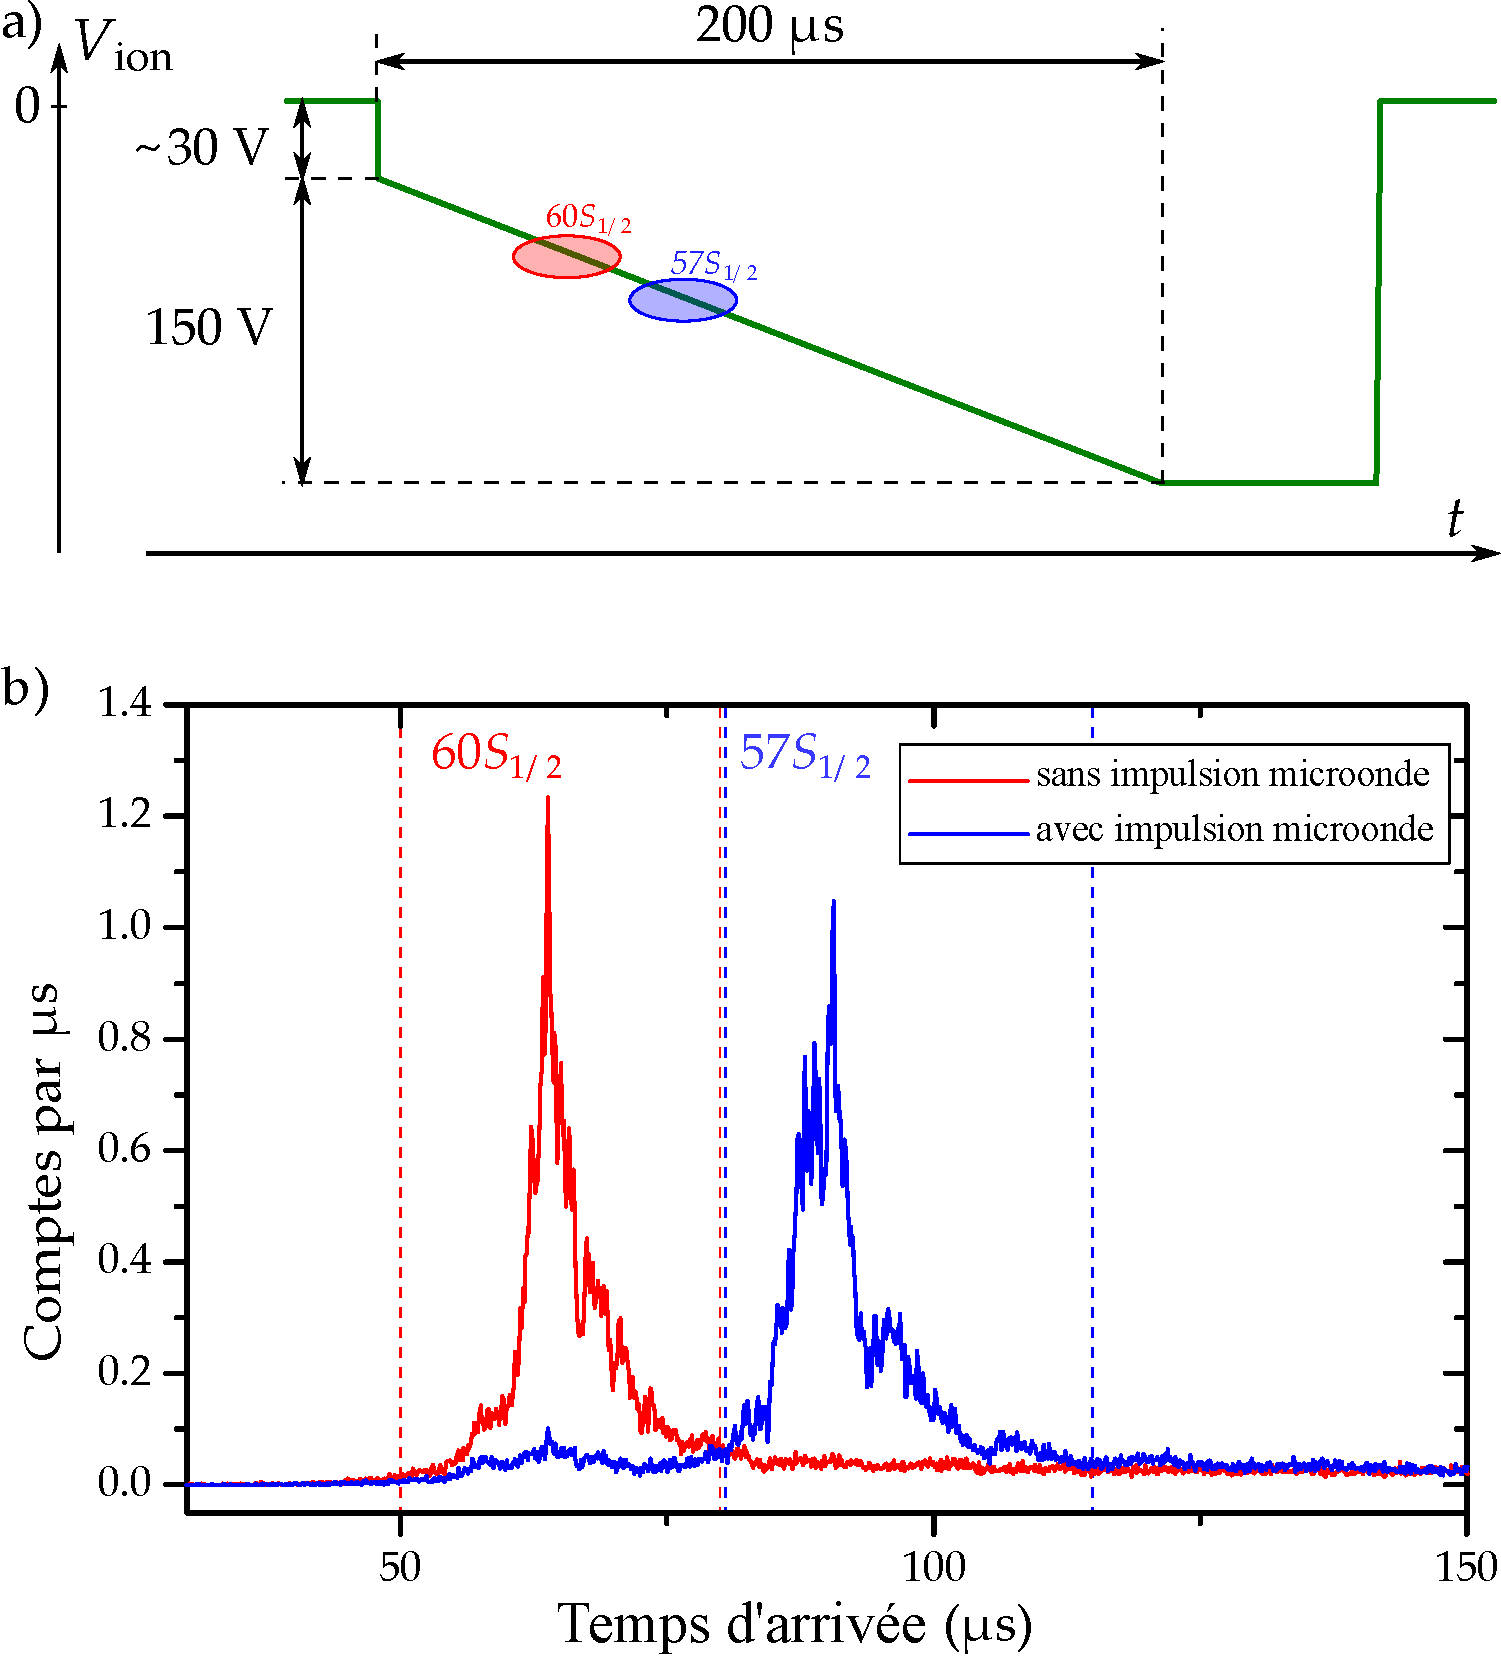
\includegraphics[width=.7\linewidth]{figures/setup/rydberg/arrTimes6057}
\caption[Détection sélective des niveaux $\mathrm{60S_{1/2}}$ et $\mathrm{57S_{1/2}}$]{
Détection sélective des atomes de Rydberg.
\textbf{a)} Une rampe de tension $V_{ion}$ typique appliquée sur les électrodes d'ionisation.
Les seuils d'ionisation des niveaux $\mathrm{60S_{1/2}}$ et $\mathrm{57S_{1/2}}$ sont indiqués en rouge et bleu respectivement.
\textbf{b)} Temps d'arrivée des ions correspondants. Des fenêtres temporelles de détection, représentées en pointillés, sont définies pour compter sélectivement les atomes dans les niveaux $\mathrm{60S_{1/2}}$ et $\mathrm{57S_{1/2}}$.
Les atomes sont préparés dans l'état $\mathrm{60S_{1/2}}$ et le niveau $\mathrm{57S_{1/2}}$ est peuplé par une impulsion $\pi$ de la transition microonde adéquate.
Les échelles de temps sont différentes en \textbf{a)} et \textbf{b)}.
}
\label{fig:arrTimes6057}
\end{figure}
%


\newpage		
\subsection{Les champs électriques parasites, défi des atomes de Rydberg sur puce}\label{subsec:flashRb}
	%problème des champs électriques et flash de Rb}
\noindent Comme nous l'avons dit au chapitre \ref{chapter:Rydberg}, les atomes de Rydberg sont des objets extrêmement sensibles au champ électromagnétique.
Or, dans notre expérience, nous souhaitons exciter et manipuler des atomes de Rydberg à proximité immédiate d'une surface, la puce à atomes.
Les champs électriques parasites étant inévitables près d'une surface, la présence de la puce va rendre difficile l'excitation et la manipulation des atomes de Rydberg.

\subsubsection*{Premiers spectres}
\noindent Ce problème est très clair sur les premiers spectres optiques que nous avons fait de la transition $\ket{\mathrm{5S_{1/2}}} \rightarrow \ket{\mathrm{60S_{1/2}}}$, présentés en figure \eqref{fig:vieilles_raies}.
%
\begin{figure}[!h]
\centering
\includegraphics[width=.8\linewidth]{figures/setup/rydberg/vieilles_raies}
\caption[Spectres d'excitation laser 5S-60S avant le dépôt de rubidium sur la puce]{
Deux spectres laser de la transition $5\mathrm{S}\rightarrow60\mathrm{S}$, avant correction des inhomogénéités et de la dérive du champ électrique.
Leurs largeurs sont de $\SI{30}{\MHz}$ et $\SI{40}{\MHz}$ respectivement, et ils sont décalés en fréquence de $\SI{12}{\MHz}$ l'un par rapport à l'autre.
Les deux spectres ont été pris dans les mêmes conditions, à \SI{1}{\hour} d'intervalle, pendant laquelle un MOT était piégé devant la puce.
L'origine de l'axe des abscisses correspond à la fréquence résonante de la transition $\mathrm{5S}\rightarrow\mathrm{60S}$ en l'absence de champ électrique.
}
\label{fig:vieilles_raies}
\end{figure}
%
Ces premiers spectres présentent des largeurs de raie de plusieurs dizaines de $\si{\MHz}$, et une forme asymétrique caractéristique d'un élargissement Stark inhomogène.
De plus, une heure de fonctionnement de l'expérience cause un déplacement en fréquence de la raie de \SI{12}{\MHz}.

Cet effet est causé par la variation spatiale et temporelle du champ électrique dans la région du nuage atomique :
%L'énergie des niveaux de Rydberg dépend fortement du champ électrique extérieur au niveau de chaque atome.Ainsi, 
si les atomes dans différentes régions du nuage voient des champs électriques différents, la fréquence de la transition $\mathrm{5S}\rightarrow\mathrm{60S}$ sera déplacée différemment dans chaque région par l'effet Stark, et la raie spectrale s'en trouvera élargie.
Une largeur de raie de $\SI{40}{\MHz}$ correspond à un champ électrique variant de $\SIrange{0}{0.667}{\V/\cm}$ sur l'extension du nuage, d'après les coefficients Stark donnés en table \ref{tab:Stark_60S}.
Or le nuage utilisé pour ces spectres était un MOT de $\sim \SI{200}{\um}$ de diamètre, ce qui nous donne une valeur de gradient de champ électrique de l'ordre de $\SI{35}{(\V/\cm)\per\cm}$.


%\clearpage
\subsubsection*{Potentiel de contact du rubidium sur l'or et dépôt contrôlé}
\noindent La cause principale de l'inhomogénéité spatiale et temporelle des champs électriques est l'accumulation d'un dépôt d'atomes de rubidium sur la surface en or de la puce :
lorsque les atomes du piège sont relâchés à la fin de chaque séquence, une partie d'entre eux entre en contact avec la surface froide de la puce et s'y dépose.
Des dépôts volontaires d'atomes sur la puce, à partir de nuages piégés, nous ont confirmé l'importance de ce phénomène et de ses effets sur les spectres d'excitation laser.

L'accumulation d'atomes de rubidium sur la puce forme d'importants dipôles électriques.
En effet, les niveaux de Fermi de l'or et du rubidium étant différents, lorsque les deux métaux sont mis en contact les électrons se déplacent de l'un à l'autre pour équilibrer les niveaux de Fermi.
Un potentiel électrostatique de contact est alors créé entre l'or et le rubidium.
La surface de la puce étant mise à la masse, ce sont les plaques de rubidium déposé qui se chargent à $\SI{2.5}{\V}$ environ.
Or le dépôt de rubidium depuis les nuages piégés est un processus lent et non contrôlé, sur des échelles de longueur de l'ordre du $\si{\mm}$.
Cela a pour conséquence un champ électrique variant dans le temps et inhomogène à une distance de la puce inférieure à quelques $\si{\mm}$.
C'est justement là que se trouvent les atomes piégés que l'on souhaite exciter.

La solution que nous avons mise en \oe uvre fut de saturer le dépôt de rubidium sur la puce, en faisant un dépôt contrôlé macroscopique sur une surface grande devant la région de piégeage.
Pour que cela fonctionne, il est important que le rubidium déposé reste métallique, non oxydé, et ne migre pas dans le cryostat en raison de différences de températures.
Ces contraintes nous ont décidés à faire le dépôt de rubidium à froid, lorsque le cryostat est sous vide et thermiquement stable.
Le dépôt contrôlé a été réalisé grâce à l'installation de dispenseurs de rubidium dans le cryostat, orientés de façon à pouvoir couvrir la puce de rubidium métallique.
La figure \eqref{fig:depotRb} illustre qualitativement la structure des champs électriques au voisinage de la puce avant et après le dépôt de rubidium.
Les dispenseurs nous ont permis de déposer une couche de rubidium, estimée à environ $\SI{80}{\nano\meter}$ d'épaisseur, sur une partie importante de la surface de la puce.

%
\begin{figure}[h]
\centering
\includegraphics[width=\linewidth]{figures/setup/rydberg/depotRb}
\caption[Dépôt contrôlé de rubidium sur la puce]{
Schéma illustrant les dépôts de rubidium sur la puce et les champs électriques qui en résultent.
Les dépôts de rubidium sont représentés en rouge et les traits gris fléchés représentent les lignes de champ électrique.
Les surfaces représentées en jaune (puce et électrode d'ionisation) sont mise à la masse.
L'ovale orange représente la position du nuage atomique (les échelles ne sont pas respéctées).
\textbf{a)} Dépôt non-contrôlé dû aux atomes piégés : le champ électrique est inhomogène et varie dans le temps.
\textbf{b)} Dépôt contrôlé réalisé grâce aux dispenseurs de rubidium (indiqués par les cercles rouges) : le champ électrique créé par le potentiel de contact rubidium-or est homogène et stable dans le temps.
}
\label{fig:depotRb}
\end{figure}
%

\clearpage
Un spectre d'excitation laser enregistré juste après ce dépôt de rubidium dans un MOT à $\SI{500}{\um}$ de la puce est présenté en figure \eqref{fig:raiefine_depot}.
Les conditions d'excitation sont similaires à celles des spectres présentés en figure \eqref{fig:vieilles_raies}, mais la largeur de raie spectrale est de seulement $\Delta\nu=\SI{1.7}{\MHz}$.
Le dépôt de rubidium a donc eu un effet extrêmement bénéfique sur l'excitation d'atomes de Rydberg au voisinage de la puce.

Des optimisations ultérieures des conditions d'excitation nous ont permis d'obtenir des raies spectrales d'une largeur de $\Delta\nu \simeq \SI{625}{\kHz}$, que nous attribuons majoritairement à une fluctuation lente de la fréquence des lasers \cite{PHD_CELISTRINO}.

\begin{figure}[h]
\centering
\includegraphics[width=\linewidth]{figures/setup/rydberg/avant-apres-coating}
%setup/rydberg/raiefine_depot}
\caption[Spectres d'excitations laser 5S-60S avant et après le dépôt de rubidium sur la puce]{
Spectres d'excitations laser 5S-60S d'atomes piégés dans un MOT, juste avant (noir et rouge) et juste après (bleu) le dépôt de rubidium sur la puce.
L'insert reprend le spectre bleu à une échelle plus adaptée.
L'ajustement gaussien donne une largeur de $\Delta\nu=\SI{1.7}{MHz}$ :
la largeur de raie a été considérablement réduite par le dépôt contrôlé de rubidium.
}
\label{fig:raiefine_depot}
\end{figure}


%\clearpage	
\subsection{Contrôle du champ électrique perpendiculaire à la puce}\label{subsec:compensation}
\noindent Le dépôt saturé de rubidium sur la puce nous a permis de réduire considérablement les inhomogénéités de champ électrique.
% mais ne garantit en rien un champ nul
Nous souhaitons néanmoins pouvoir contrôler la valeur moyenne du champ à la position du nuage atomique, dans deux optiques.
La première est la réduction de l'effet des inhomogénéités résiduelles.
En effet, en raison de la forme quadratique de l'effet Stark, plus la valeur moyenne du champ électrique est élevée, plus la raie spectrale sera élargie par une même variation autour de la valeur moyenne.
Pour des valeurs de champ électrique comprises entre $F-\Delta F$ et $F + \Delta F$, l'élargissement de la raie spectrale vaut
%
\begin{equation}
\label{eq:Stark_broadening}
\begin{aligned}
\nu(F-\Delta F) - \nu(F+\Delta F) &= A (F-\Delta F)^2 - A (F-\Delta F)^2 \\
&= A\cdot [(F-\Delta F)^2 - (F+\Delta F)^2] \\
&= -4A \cdot F\cdot \Delta F
\end{aligned}
\end{equation}
%Cela se conçoit fort bien à l'observation de la figure \eqref{fig:Stark_60S}.

La seconde optique d'un contrôle plus fin du champ électrique est de pouvoir déplacer en fréquence %la transition laser vers les niveaux de Rydberg ainsi que 
les transitions microonde entre niveaux de Rydberg voisins.
Cet aspect du contrôle des champs électriques nous sera surtout utile lorsque nous nous intéresserons aux niveaux de Rydberg circulaires, dans les chapitres \ref{chapter:circsim} et \ref{chapter:50c}.
	
Le moyen le plus direct dont nous disposons pour le contrôle du champ électrique est l'application d'une tension sur les électrodes d'ionisation $I_1$ et $I_2$ représentées en figure \eqref{fig:schema_detect}.
Il est raisonnable de supposer, étant donnée la grande surface de ces électrodes, que le champ créé entre celles-ci et la puce est homogène spatialement, au moins là où se situe le nuage atomique.
Le contrôle de la tension appliquée à ces électrodes présente une exigence technique particulière :
%demande un certain raffinement technique :
nous voulons contrôler le champ électrique vu par les atomes à l'échelle de la dizaine de $\si{\mV/\cm}$, tout en étant capable d'appliquer une tension de quelques centaines de Volts sur les mêmes électrodes afin d'ioniser et détecter les atomes de Rydberg.

Nous avons pour cela conçu un circuit électronique permettant de commuter rapidement la tension appliquée aux électrodes, entre une voie basse tension à bas bruit pendant l'excitation des atomes de Rydberg et une voie haute tension servant à leur détection.
Ce circuit est schématisé en figure \eqref{fig:detectionbox_ENS}.
%
\begin{figure}[!h]
\centering
\includegraphics[width=.8\linewidth]{figures/setup/rydberg/detectionbox_ENS}
\caption[Circuit de contrôle de la tension des électrodes d'ionisation]{
Circuit de contrôle de la tension des électrodes d'ionisation.
Les tensions sont fournies par un générateur de fonctions arbitraires contrôlé par ordinateur, puis amplifiées par un amplificateur haute tension de gain $\times \num{50}$, délvrant jusqu'à $\pm \SI{150}{\V}$.
Pendant l'excitation des atomes de Rydberg, l'optocoupleur est bloquant.
Le pont diviseur de tension créé par la résistance de $\SI{50}{\kilo\ohm}$ d'une part et de $\SI{2.5}{} + \SI{4.7}{\kilo\ohm}$ divise par un facteur $\num{8}$ le bruit électronique au niveau des électrodes, au prix d'une réduction d'autant du signal.
Pendant la phase de détection, l'optocoupleur est passant et le pont diviseur est ainsi court-circuité.
La tension appliquée aux électrodes est alors directement la tension en sortie de l'amplificateur.
}
\label{fig:detectionbox_ENS}
\end{figure}
%

%\clearpage
\subsection{Manipulation cohérente des états de Rydberg}\label{subsec:mw_spectro}

\noindent Nous avons jusqu'ici limité notre exposé à l'excitation laser d'atomes vers un niveau de Rydberg déterminé.
Or nos expériences reposent sur la manipulation des atomes de Rydberg entre plusieurs états, en vue de deux objectifs.
Le premier est la caractérisation des interactions entre niveaux de Rydberg et le second est le développement d'un système quantique pouvant servir de plateforme pour la simulation quantique.

Les différences d'énergie entre niveaux de Rydberg voisins, comme nous l'avons évoqué au chapitre \ref{chapter:Rydberg}, sont dans le domaine des microondes millimétriques.
Cela correspond grossièrement à des fréquences de transition de l'ordre de $\SI{10}{}$ à $\SI{100}{\GHz}$.
La spectroscopie de ces transitions (\og spectroscopie microonde \fg{}) est l'outil majeur dont nous disposons pour caractériser les atomes de Rydberg au-delà de la spectroscopie laser de la transition depuis le niveau fondamental.
Son application pour l'étude du mouvement d'un nuage dense d'atomes de Rydberg sera discutée à la fin du chapitre \ref{chapter:60s}.
Son application à l'étude des atomes de Rydberg circulaires et à leur manipulation cohérente sera discutée aux chapitres \ref{chapter:circsim} et \ref{chapter:50c}.

Ici, nous évoquerons la manipulation cohérente d'un \og qubit de Rydberg \fg{} réalisé entre les états $\mathrm{60S}$ et $\mathrm{61S}$, ainsi que l'utilisation de la spectroscopie de la transition $\mathrm{60S} \rightarrow \mathrm{60P}$ pour mesurer les champs électriques résiduels.
Ces deux expériences 
%ont été menées avant l'installation des électrodes RF, et avec le premier circuit de contrôle du champ électrique (cf. \ref{subsec:compensation}). Elles 
sont décrites en détail dans la thèse de Carla Hermann Avigliano \cite{PHD_HERMANN}.

%\clearpage
\subsubsection*{Un qubit de Rydberg d'une grande longévité}
\noindent Au sein de notre dispositif, la cohérence d'un système quantique à deux niveaux réalisé entre deux niveaux de Rydberg est limitée en premier lieu par l'inhomogénéité du champ électrique résiduel.
De bons candidats à la réalisation d'un tel qubit seront donc des niveaux dont la sensibilité au champ sera la plus faible possible ou, à défaut, la plus similaire possible.
Les coefficients d'effet Stark quadratique synthétisés en table \eqref{tab:Stark_60S} nous éclairent dans notre choix : nous utiliserons les niveaux $\mathrm{60S_{1/2}}$ et $\mathrm{61S_{1/2}}$.
La quantité pertinente ici est le décalage en fréquence de la transition par l'effet Stark différentiel entre ces deux niveaux.
Celui-ci vaut $A_{\mathrm{60S1/2,61S1/2}} = \SI{-11}{\MHz \per (\V \per\cm) \squared}$.
La spectroscopie de la transition $\ket{g}=\ket{\mathrm{60S_{1/2},m_j=1/2}} \rightarrow \ket{e}=\ket{\mathrm{61S_{1/2},m_j=1/2}}$ est présentée en figure \eqref{fig:spectro_60S61S}.

La largeur de raie de $\Delta\nu=\SI{6.6}{\kHz}$ est de bon augure pour la manipulation cohérente de ce qubit.
Afin d'estimer son temps de cohérence de façon plus précise, nous avons effectué une spectroscopie Ramsey avec écho de spin entre les deux niveaux, dont le principe est schématisé en figure \eqref{fig:spinEcho_60S61S}.

\begin{figure}[h]
\centering
\vspace{1em}
\includegraphics[width=.8\linewidth]{figures/setup/rydberg/spectro_60S61S}
\caption[Spectroscopie de la transition 60S-61S]{
Spectroscopie de la transition 60S-61S.
\textbf{a)} Diagramme de niveaux de la transition microonde à deux photons.
\textbf{b)} Spectre micro-onde de la transition, pour une durée d'excitation de $\SI{300}{\us}$. La courbe rouge est un ajustement lorentzien.
}
\label{fig:spectro_60S61S}
\end{figure}

\begin{figure}[!h]
\centering
\vspace{1em}
\includegraphics[width=.8\linewidth]{figures/setup/rydberg/spinEcho_60S61S}
\caption[Écho de spin 60S-61S]{
Spectroscopie Ramsey avec écho de spin sur la transition 60S-61S.
\textbf{a)} Principe de l'écho de spin représenté sur la sphère de Bloch. $\ket{g}$ et $\ket{e}$ représentent les états $\mathrm{60S_{1/2}}$ et $\mathrm{61S_{1/2}}$ respectivement.
\textbf{b)} Contraste des franges de Ramsey avec écho de spin, en fonction de la durée de $T$ de l'intervalle d'évolution. La courbe rouge est un ajustement gaussien.
}
\label{fig:spinEcho_60S61S}
\end{figure}

\newpage
La technique d'écho de spin permet de se libérer des sources de décohérence stables dans le temps, telles que l'inhomogénéité spatiale du champ électrique.
L'impulsion $\pi$ intercalée à la moitié de l'évolution de la superposition d'état agit comme un renversement du temps.
Les effets de déphasage de la superposition ne variant pas dans le temps sont ainsi compensés dans la deuxième moitié de son évolution.
L'ajustement gaussien du contraste des franges de Ramsey en fonction du temps total d'évolution permet d'extraire un temps de cohérence à $1/e$ de la superposition de $T_2 = \SI{631}{\us}$.
Ce temps de cohérence est trois fois supérieur à la durée de vie des niveaux de Rydberg, qui est de l'ordre de $\SI{200}{\us}$.
Cela signifie que, alors que la plupart des atomes de Rydberg ont été perdus par désexcitation radiative, ceux qui ne l'ont pas été, donc ceux que nous détectons, gardent leur cohérence pendant une durée $T_2$.

%\clearpage
\subsubsection*{Mesure des champs électriques résiduels}
\noindent La même technique de spectroscopie microonde nous a permis de mesurer les champs électriques résiduels.
Pour cela, à l'inverse de l'expérience précédente, nous voulions une transition aussi sensible que possible à l'effet Stark.
Nous avons donc choisi la transition $\mathrm{60S}\rightarrow\mathrm{60P}$., qui présente un effet Stark quadratique de .
Celle-ci se sépare par effet Zeeman entre les transitions $\mathrm{60S_{1/2},m_j=1/2} \rightarrow \mathrm{60P_{3/2},m_j=-1/2}$ %, présentant un effet Stark différentiel de $\SI{586.1}{\MHz \per (\V \per\cm) \squared}$ 
et $\mathrm{60S_{1/2},m_j=1/2} \rightarrow \mathrm{60P_{3/2},m_j=+3/2}$, qui présentent des effets Stark différentiels de $\SI{586.1}{}$ et $\SI{479.1}{\MHz \per (\V \per\cm) \squared}$ respectivement.
%Les atomes étant piégés dans le piège magnétique, l'effet Zeeman est ici important.
%En particulier, c'est le champ magnétique qui détermine l'axe de quantification, et donc l'axe de symétrie de la fonction d'onde des niveaux $P$.
%Pour cette raison, un champ électrique parallèle au champ magnétique produira un déplacement d'énergie par effet Stark différent d'un champ électrique perpendiculaire au champ magnétique.
L'anistropie des niveaux $P$ en présence d'un champ magnétique, ici celui qui sert à piéger les atomes, nous a permis d'estimer indépendamment le champ électrique résiduel perpendiculairement et parallèlement à la puce.
Le champ résiduel perpendiculaire à la puce a été mesuré à $\SI{0.09}{\V/cm}$, cette valeur pouvant être compensée par l'application d'une tension sur les électrodes d'ionisation.
Le champ parallèle à la puce a été mesuré à $\SI{0.09}{\V/cm}$ à $\SI{150}{\um}$ de la puce, décroissant jusqu'à des valeur comprise entre $\SI{0.05}{}$ et $\SI{0.06}{\V/\cm}$ pour des distances à la puce supérieures à $\SI{300}{\um}$.
Ce champ résiduel parallèle à la puce ne pourra être compensé qu'après installation des électrodes RF.

Enfin, cette expérience nous a permis d'estimer les gradients résiduels du champ électrique au voisinage de la puce, à partir de la taille du nuage et de la largeur des raies spectrales de transition, principalement due à un élargissement Stark inhomogène, tel que présenté en \ref{subsec:flashRb}.
Ces estimations ont été faites dans l'approximation d'un gradient de champ constant et principalement situé sur la composante $F_x$.
La table \ref{tab:fieldGrad} synthétise ces mesures.
%
\begin{table}[!h]
	\centering
	\caption[Estimation des gradients de champ électrique près de la puce]{Gradient de champ électrique au voisinage de la puce, à différentes distances.%, selon les directions $x$ et $z$.
	}
	\label{tab:fieldGrad}
	\begin{tabular}{c c c}
		\toprule\midrule
		Distance à la puce
		& $\partial |F| / \partial x$
		& $\partial |F| / \partial z$\\		
		$\si{\um}$
		& $\si{(\V/\cm\squared)}$
		& $\si{(\V/\cm\squared)}$\\
		\midrule
		\SI{150}{} & \SI{1.428}{} & \SI{21.714}{} \\
		\SI{245}{} & \SI{1.504}{} & \SI{9.023}{} \\
		\SI{338}{} & \SI{2.166}{} & \SI{11.597}{} \\
		\SI{455}{} & \SI{1.566}{} & \SI{9.011}{} \\
		\SI{555}{} & \SI{0.9}{} & \SI{5.088}{} \\
		\SI{675}{} & \SI{0.76}{} & \SI{4.277}{} \\
		\midrule
		\bottomrule
 	\end{tabular}
\end{table}
%

Nous pouvons en déduire que la distance à la puce à laquelle nous choisissons de placer les atomes de Rydberg aura une influence déterminante sur leur exposition à un effet Stark inhomogène.

\subsection{Temps de vie des atomes de Rydberg et température effective}\label{subsec:lifetime}
\noindent Nous avons calculé, au chapitre \ref{chapter:Rydberg}, la durée de vie du niveau $\mathrm{60S}$ à différentes températures.
La figure \ref{fig:lifetime_60S} montre une mesure expérimentale du nombre d'atomes de Rydberg détectés dans le nuage atomique, en fonction du délai entre l'excitation et la détection des atomes de Rydberg.

L'ajustement exponentiel de cette mesure donne un temps de vie de $\tau_{\mathrm{60S}} = \SI{210}{} \pm \SI{4}{\us}$, alors que le temps de vie théorique calculé à la température de l'hélium liquide vaut $\SI{239.8}{\us}$ (cf table \ref{tab:lifetime_60S}).
La différence de temps de vie peut s'expliquer par différents effets :
les atomes sont exposés au rayonnement du corps noir à température ambiante et à la température de l'azote liquide, qui peut entrer par les hublots d'accès optique.
De plus, la géométrie complexe des surfaces conductrices au voisinage des atomes (puce et électrodes) changent la densité de mode du rayonnement électromagnétique par rapport à celle du vide.

Afin de rendre compte simplement de ces effets, nous calculons une température effective.
C'est la température pour laquelle le calcul du temps de vie théorique présenté au chapitre \ref{chapter:Rydberg} donnerait la valeur de temps de vie mesurée.
Cette température effective pour le niveau $\mathrm{60S}$ dans notre cryostat est de $\SI{36}{\kelvin}$.

\begin{figure}[h]
\centering
\includegraphics[width=0.8\linewidth]{figures/setup/rydberg/lifetime_60S}
\caption[Durée de vie du niveau 60S]{
Nombre d'atomes de Rydberg dans le niveau $\mathrm{60S}$ détectés, en fonction du délai entre l'impulsion laser d'excitation et la rampe d'ionisation servant à leur détection.
L'ajustement exponentielle donne un temps de vie de $\SI{210}{} \pm \SI{4}{\us}$.
}
\label{fig:lifetime_60S}
\end{figure}

\section*{Conclusion}
\noindent Nous avons, dans le présent chapitre, décrit le fonctionnement du dispositif expérimental sur lequel nous avons effectué nos travaux.
Le dispositif cryogénique et la puce à atomes nous permettent de piéger et refroidir des nuages d'atomes de \Rb{87} jusqu'à la condensation de Bose-Einstein.
Un second aspect du dispositif nous permet d'exciter, manipuler et détecter des atomes de Rydberg au sein de ces nuages d'atomes ultra-froids.

La difficulté particulière que présente la manipulation d'atomes de Rydberg près d'une surface, due à leur très grande sensibilité au champ électromagnétique, a été surmontée par le dépôt contrôlé d'une couche macroscopique de rubidium sur la surface de la puce atomique.
Ce dépôt garantit en effet une bonne homogénéité des champs électriques résiduels, mise en évidence par l'étroitesse des raies de transition optique et par la longévité du qubit de Rydberg réalisé entre les niveaux $\mathrm{60S}$ et $\mathrm{61S}$.

Nous disposons ainsi 
%, malgré ses fortes exigences techniques,
d'un dispositif performant et prometteur pour l'étude des interactions entre atomes de Rydberg.
% froids.
%\chapter{Des atomes de Rydberg froids en environnement cryogénique}
\label{chapter:setup_coldatoms_Rydberg}
%
%INTRODUCTION DU CHAPITRE\\
%entre autres, longue vie aux Rydberg en environnement cryogénique

\noindent L'observation d'atomes de Rydberg en interaction sur des temps longs, tant pour la question du mouvement d'un gaz de Rydberg ultra-froids que dans l'optique de la simulation quantique, requiert des conditions expérimentales spécifiques.
D'une part, il est souhaitable que la durée de vie des niveaux de Rydberg soit la plus longue possible, ce qui nous pousse à travailler en environnement cryogénique.
Les calculs menés dans le chapitre \ref{chapter:Rydberg} nous montrent l'importance de la température de l'environnement sur la durée de vie des atomes de Rydberg, plus cruciale encore si l'on souhaite travailler avec des atomes de Rydberg circulaires.

D'autre part, il est nécessaire, étant donnés nos objectifs, que nos atomes de Rydberg soient aussi froids que possible.
L'on pourrait imaginer piéger et refroidir des atomes qui auraient été préalablement excités dans des niveaux de Rydberg à partir d'un jet atomique chaud.
Cependant, il n'y a pas de technique connue à ce jour qui permette cela, et la durée de vie des niveaux de Rydberg en limiterait très certainement les possibilités.
Or les techniques de piégeage et de refroidissement des atomes alcalins non excités sont des outils bien maîtrisés.
Voilà donc une piste bien plus prometteuse.

Une première difficulté se présente ici : les techniques d'atomes ultra-froids sont pour la plupart développées au sein de dispositifs à température ambiante.
Il s'agira donc ici de les concilier avec un environnement cryogénique.
Avec cette contrainte à l'esprit, et dans l'optique d'obtenir des nuages atomiques très confinés, il a été choisi de centrer le dispositif autour d'une puce à atomes supraconductrice.
Prenons note dès maintenant d'une deuxième difficulté technique posée par un tel dispositif :
les atomes de Rydberg sont extrêmement sensibles au champ électromagnétique, et nous souhaitons les exciter et les observer au voisinage de la surface conductrice qu'est notre puce atomique.

Ce chapitre sera donc dédié à la description du dispositif expérimental sur lequel nous avons effectué nos travaux.
Nous nous intéresserons d'abord à l'aspect du dispositif qui nous sert à piéger et refroidir des atomes de \Rb{87} sur une puce atomique supraconductrice.
Nous nous attacherons ensuite à décrire comment nous excitons, manipulons et détectons les atomes de Rydberg au sein de ce dispositif.

\section{Un nuage d'atomes ultra-froids sur puce, du MOT de capture au condensat de Bose-Einstein}

\noindent Le développement de notre plateforme d'atomes froids autour d'une puce supraconductrice a été l'objet de plusieurs thèse de doctorat précédant celle-ci.
Les thèses de Thomas Nirrengarten \cite{PHD_NIRRENGARTEN}, de Cédric Roux \cite{PHD_ROUX} et d'Andreas Emmert \cite{PHD_EMMERT} sont dédiées à la question du piégeage et du refroidissement jusqu'au BEC d'atomes de \Rb{87} près d'une surface à l'aide de fils supraconducteurs.
La thèse de Raul Celistrino Teixeira \cite{PHD_CELISTRINO} détaille la fabrication et les caractéristiques de la puce atomique que nous avons utilisée pour nos expériences.

Nous ferons donc ici une présentation rapide du cryostat et de la puce à atomes que nous utilisons, puis nous détaillerons la suite d'étapes que nécessite le piégeage et le refroidissement des atomes de rubidium au sein de notre dispositif.
Enfin, après avoir présenté la technique d'imagerie atomique par absorption, nous présenterons quelques chiffres typiques de nos nuages atomiques.


	\subsection{L'environnement cryogénique : cryostat et puce à atomes supraconductrice}\label{subsec:cryopuce}
	
\noindent L'environnement cryogénique présente un avantage incomparable pour la durée de vie des atomes de Rydberg, mais impose aussi quelques spécificités à notre dispositif d'atomes froids.
Le piégeage d'atomes froids pendant des durées suffisantes à leur manipulation exige un vide très poussé dans l'enceinte expérimentale, car les collisions avec les molécules de gaz résiduel éjectent les atomes hors de leur piège.
Les chambres de piégeage d'atomes neutres à température ambiante sont généralement étuvées pendant plusieurs semaines afin d'atteindre des pressions de gaz résiduel suffisamment faibles.
Dans un environnement cryogénique au contraire, les parois froides de l'enceinte adsorbent une grande partie du gaz résiduel, et des pressions très inférieures à \SIvv{1e-10}{\milli\bar} sont obtenues sans étuvage.
Travailler en environnement cryogénique permet en outre l'utilisation de fils et de bobines supraconducteurs pour le passage des courants électriques qui génèrent les champs magnétiques nécessaires au piégeage des atomes.
Des courants de quelques Ampères sont ainsi passés sans dissipation et à proximité des atomes piégés, alors qu'une expérience d'atomes froids à température ambiante nécessite des bobines qui soient placées en-dehors de la chambre et refroidies par des circuits d'eau dédiés.

L'environnement cryogénique pour les atomes froids a cependant quelques inconvénients :
en premier lieu, l'accès optique est limité car les parois de l'enceinte doivent être opaques pour le rayonnement du corps noir et donc métalliques, chaque hublot de verre réduisant l'isolation thermique du c\oe ur de l'expérience.
En second lieu, l'utilisation d'hélium et d'azote liquide à proximité d'un vide poussé présente une lourdeur technique supplémentaire au quotidien.

	\subsubsection*{Le cryostat}
\noindent Notre expérience est placée au c\oe ur du cryostat représenté en figure \eqref{fig:cryo}.
%
\begin{figure}
\centering
\includegraphics[width=\linewidth]{figures/setup/coldatoms/cryo_vect.jpg}
\caption[Schéma du cryostat]{Schéma du dispositif cryogénique :
\textbf{a)} Coupe du du cryostat, avec la puce tournée vers le côté gauche.
Le réservoir d'azote liquide est indiqué en jaune, le réservoir d'hélium liquide en bleu.
Le c\oe ur de l'expérience est visible, ainsi que les deux \og jupes \fg{} et l'enceinte extérieure à température ambiante.
Cinq hublots, trois en face de la puce et un sur chaque côté, sont installés sur chacune de ces jupes pour l'accès optiques.
\textbf{b)} Vue schématique du c\oe ur de l'expérience. La puce fait face à la direction $y$. Les bobines (vert foncé), le channeltron et les différentes électrodes sont représentées. On ne voit pas les \og jupes \fg{} d'azote et d'hélium, ni l'enceinte extérieure.
\textbf{c)} Vue de près des bobines : la bobine QUAD (mauve) génère un champ quadrupolaire pour faire un MOT sur puce. L'emplacement de la puce est représenté par le rectangle bleu devant la bobine QUAD et la bobine $B_y$ (vert clair).
La zone rouge indique l'endroit où les atomes de rubidium sont piégés.
}
\label{fig:cryo}
\end{figure}
%
La conception de ce cryostat a été évoquée dans la thèse de Raul Celistrino Teixeira \cite{PHD_CELISTRINO}  et discutée plus en détail dans les thèses de Thomas Nirrengarten \cite{PHD_NIRRENGARTEN} et Cédric Roux \cite{PHD_ROUX}.
Le c\oe ur de l'expérience est protégé de la radiation extérieure par des écrans thermiques (\og jupes \fg{}) en cuivre doré. Ce sont des cylindres ouverts en haut et vissés sur le fond des réservoirs de liquides cryogéniques.
La jupe $^4 \text{He}$ est vissée sur le fond du réservoir d'hélium 4 et la jupe $\text{N}_2$ est vissée au fond du réservoir d'azote liquide.
Elles sont donc respectivement thermalisées à \SIvv{4.2}{\K} et \SIvv{77}{\K}.
Sur chaque jupe, cinq hublots sont installés pour l'accès optique à la zone de piégeage :
deux sur les directions $\pm x$, un dans la direction $+y$ qui fait face à la puce, et deux  dans le plan $yz$, de part et d'autre du hublot de face sur les bissectrices des axes $+y$ et $\pm z$, appelées direction $\pm\SIvv{45}{\degree}$ respectivement.
Par ces hublots, tous les faisceaux laser atteignent la zone de piégeage au c\oe ur de l'expérience.
Tous les éléments qui sont installés à l'intérieur de la jupe hélium sont thermalisés à \SIvv{4.2}{K} par contact thermique avec le réservoir d'hélium liquide.

L'intérieur de la jupe hélium est revêtu d'une couche de plomb, supraconducteur à \Khe. Cette couche de plomb écrante les champs magnétiques extérieurs par effet Meissner \cite{MX_MEISSNEREFFECT}, et évite les courants de Foucault qui se créeraient dans les jupes en cuivre à l'allumage ou à l'extinction des courants dans les bobines. 
Il reste nécessaire cependant d'imposer un champ extérieur de compensation au moment du refroidissement, afin que la couche de plomb ne piège pas de lignes de champ magnétique provenant de l'environnement.
Cette compensation du champ constant de l'environnement est réalisée à l'aide de grandes bobines placées à l'extérieur du crysotat.

Enfin, bien que les jupes ne soient pas parfaitement étanches, elles garantissent un vide différentiel entre la partie du cryostat à \SIvv{300}{\K}, où la pression vaut \SIvv{1.5e-7}{\milli\bar}, et la partie à \Khe, où la pression est inférieure à \SIvv{1e-10}{\milli\bar}\footnote{
Cette valeur n'est pas mesurée en raison de l'absence de sonde de pression dans cette région du cryostat, mais inférée à partir du temps de vie des nuages d'atomes piégés, qui est de l'ordre de la minute \cite{ENS_CHIPLIFETIME}.}.

	\subsubsection*{La puce à atomes}
\noindent La puce à atome qui siège au c\oe ur de notre expérience est représentée en figure \eqref{fig:chip}.
C'est une puce assez simple, conçue autour de trois fils supraconducteurs : le fil (LJ), en forme de \mcal{U}, le fil (LG) en forme de \mcal{Z}, et le fil (KM) droit.
Ces fils sont fabriqués par dépôt de niobium d'une épaisseur de \SIvv{2}{\um} sur un substrat de silicium recouvert d'une couche d'oxyde SiO$_2$.
Le dépôt de niobium est ensuite gravé, et l'ensemble de la puce est recouvert d'une couche d'or de \SIvv{200}{\nm} d'épaisseur afin de rendre la surface réfléchissante.
Le niobium étant supraconducteur à $\SI{4.2}{\K}$, les courants électrique pourront toujours passer par les fils de la puce et non par la couche d'or qui reste dans un de état conducteur normal.
Les détails de la fabrication de la puce sont présentés en annexe dans la thèse de Raul Celistrino Teixeira \cite{PHD_CELISTRINO}.
%
\begin{figure}[!h]
\centering
\includegraphics[width=\linewidth]{figures/setup/coldatoms/chip}
\caption[Schéma de la puce à atomes supraconductrice]{Schéma de la puce supraconductrice.
Les lettres étiquettent les pattes d'entrée/sortie des courants électriques sur la puce.
Les couleurs sont une aide visuelle pour mieux suivre les fils : en vert, le \og fil \mcal{U}\fg{}, en orange le \og fil \mcal{Z}\fg{} et en bleu le \og fil RF \fg{}.
\`A droite, vue de près du centre de la puce, qui détaille la largeur des fils, la distance entre eux et le sens de circulation des courants.
Les axes $x,y$ et $z$ coïncident avec ceux de la figure \eqref{fig:cryo}.
}
\label{fig:chip}
\end{figure}
%

Les fils en \mcal{U} et en \mcal{Z} sont la simplification d'un dispositif en forme de $\mathcal{H}$ qui repose sur la circulation d'un courant perpendiculairement à deux autres courants parallèles entre eux.
La figure \eqref{fig:magfields_chip} représente les différentes configurations de champ magnétique créées par les fils \mcal{U} et \mcal{Z} de la puce.
Lors du passage d'un courant $I$ dans le fil \mcal{Z}, le segment parallèle à l'axe $x$ crée un champ qui, superposé avec un champ de biais $B_Z$ selon l'axe $z$, forme un champ quadrupolaire dans le plan $yz$.
Le courant dans les deux bras verticaux circule dans le même sens et crée un champ selon $x$, avec un  minimum non-nul au voisinage du centre du champ quadrupolaire.
Le champ total forme alors un piège magnétique de Ioffe-Pritchard (cf figure \ref{fig:magfields_chip}c)).

De façon similaire, le fil en \mcal{U} crée aussi, avec l'aide d'un champ de biais $B_Z$, un champ quadrupolaire dans le plan $yz$.
Les courants dans les bras verticaux circulent cette fois dans des sens opposés, ce qui résulte en la présence d'un zéro de champ près du centre du champ quadrupolaire.
Le champ total permet ici la réalisation d'un piège magnéto-optique sur puce en trois dimensions (\og 3D-MOT miroir\fg{}, cf figure \ref{fig:magfields_chip}d)).

\begin{figure}[]
\centering
\includegraphics[width=\linewidth]{figures/setup/coldatoms/magfields_chip}
\caption[Champs magnétiques créés par la puce]{
Champs magnétiques créés par la puce.
\textbf{a)} Les fils \mcal{U} et \mcal{Z} portent un courant dans la direction $x$ et une paire de courants parallèles dans la direction $z$.
\textbf{b)} Un champ quadrupolaire est créé par la superposition du courant selon $x$ et d'un champ de biais $B_Z$.
Les courants verticaux peuvent circuler soit (\textbf{c)}) dans le même sens,  soit (\textbf{d)}) dans des sens opposés.
Le module du champ total présente alors respectivement un minimum non-nul ou nul aux positions marquées par les points jaunes.
}
\label{fig:magfields_chip}
\end{figure}

Pour le fil en \mcal{Z} comme pour le fil en \mcal{U}, le centre du piège se situe à une distance de la puce valant approximativement
\begin{equation}
\label{eq:trap_center}
r_0 \simeq \frac{\mu _0}{2\pi}\frac{I}{B_Z}
\end{equation}
et le gradient de champ magnétique à cet endroit vaut
\begin{equation}
\label{eq:trap_center_grad}
|B'(r_0)|=\frac{2\pi}{\mu _0} \frac{B_Z^2}{I} = \frac{B_Z}{r_0} = \frac{\mu _0}{2\pi}\frac{I}{r_0^2}~.
\end{equation}
%
C'est là une caractéristique importante de la géométrie des pièges : plus le centre du piège est proche de la puce, plus le piège sera confinant dans le plan $yz$.
Le piège s'allonge alors dans la direction $x$, prenant une forme de cigare de plus en plus anisotrope.

Comme nous l'avons mentionné, notre dispositif nous permet de mettre en \oe uvre des pièges magnéto-optiques en trois dimensions.
Dans beaucoup d'expériences d'atomes froids, ceux-ci sont réalisés à l'aide de trois paires de faisceaux laser contra-propageants, une dans chaque direction de l'espace.
Il nous est impossible d'envisager cette configuration, puisque l'axe $y$ est rendu inaccessible par la présence de la puce.
L'on peut cependant, avec deux paires de faisceaux laser seulement, simuler une configuration à six faisceaux, en utilisant la surface réfléchissante de la puce.
Le schéma de cette configuration, appelée \og MOT miroir \fg{}, est donné en figure \eqref{fig:mirror_MOT}.

\begin{figure}[!h]
\centering
\includegraphics[width=0.6\linewidth]{figures/setup/coldatoms/mirror_MOT}
\caption[Schéma de principe du MOT miroir]{Schéma de principe du MOT miroir :
Deux faisceaux contra-propageants sont envoyés parallèlement à la puce réfléchissante, selon l'axe $x$.
Les deux autres faisceaux dans le plan $yz$ viennent frapper la puce avec un angle de \SIvv{45}{\degree}.
Leur réflexion sur la puce équivaut à deux faisceaux supplémentaires d'hélicité inversée, représentés en ombre derrière la puce.
On obtient bien ainsi une configuration de MOT à six faisceaux.
}
\label{fig:mirror_MOT}
\end{figure}


	\subsection{Séquence de piégeage et refroidissement}
	
\noindent Grâce à ce dispositif, nous pouvons piéger des nuages d'atomes froids sur puce.
Nous donnons dans ce paragraphe le détail des différentes étapes de piégeage et de refroidissement des atomes.

	\subsubsection*{Système laser}
\noindent Le piégeage magnéto-optique du rubidium 87 exploite la raie D2 de celui-ci.
La raie D2 est représentée en figure \eqref{fig:D2lineRb87} avec le détail des sous-niveaux hyperfins des niveaux $\mathrm{5S_{1/2}}$ et $\mathrm{5P_{3/2}}$ du \Rb{87}.
%	
\begin{figure}[!h]
\centering
\includegraphics[width=0.8\linewidth]{figures/setup/coldatoms/D2lineRb87}
\caption[Raie D2 du \Rb{87}]{Structure hyperfine de la raie D2 du \Rb{87}.
Les transitions cyclantes sont montrées pour le laser de refroidissement, le laser repompeur, le laser sonde et le laser de pompage Zeeman.
}
\label{fig:D2lineRb87}
\end{figure}
%
Nous utilisons la transition $\ket{F=2} \rightarrow \ket{F'=3}$ de la raie D2 pour piéger et refroidir les atomes.
Cette transition a une largeur naturelle $\Gamma = 2\pi \times \SI{6.065}{\MHz}$ \cite{DATA_STECKRB87}.
Le laser de refroidissement est généré par un système commercial de diode laser amplifiée TOPTICA TA-110.
La fréquence de ce laser est asservie par battement (\og beatlock \fg{}) à un laser maître, lui-même stabilisé par une cavité Fabry-Pérot.
Cette cavité est verrouillée en fréquence sur la transition de refroidissement par absorption saturée dans une cellule de \Rb{87}.
Une commande de tension permet de définir la fréquence du battement et ainsi de contrôler le désaccord du laser de refroidissement par rapport à la transition $\ket{F=2}\rightarrow\ket{F'=3}$.

Il arrive qu'un photon du laser de refroidissement excite un atome du niveau $\ket{F=2}$ vers le niveau $\ket{F'=2}$ au lieu de $\ket{F'=3}$.
Cet atome peut alors se désexciter non pas vers le niveau $\ket{F=2}$ mais vers le niveau $\ket{F=1}$, qui est un niveau noir pour le laser de refroidissement.
Afin d'éviter le pompage des atomes vers ce niveau $\ket{F=1}$, il est nécessaire d'envoyer, avec le laser de refroidissement, un laser \og repompeur\fg{} accordé sur la transition $\ket{F=1}\rightarrow \ket{F'=2}$.
Ce laser repompeur est généré par une troisième diode laser, et indépendamment verrouillé en fréquence par absorption saturée.

Deux autres fréquences laser sont utilisées dans notre expérience : les lasers de sonde, qui servent à l'imagerie atomique, et le laser de pompage Zeeman, qui sert à réaliser un pompage optique vers le niveau $\ket{F=2,m_F=+2}$.
Ces faisceaux sont prélevés sur le laser de refroidissement et décalés en fréquence par modulation acousto-optique.
L'ensemble des faisceaux est transporté de la table optique de préparation au cryostat par des fibres optiques mono-modes à maintien de polarisation.
Ils sont enfin mis en forme à proximité immédiate du cryostat. 




	\subsubsection*{Piégeage magnéto-optique}
\noindent	Notre dispositif repose sur trois stades de piégeage magnéto-optique successifs.
Les atomes de rubidium sont stockés dans une cellule en verre, ouverte vers une enceinte sous ultra-vide (UHV) située à l'extérieur du cryostat.
Le travail en environnement cryogénique nous oblige en effet à utiliser une source externe : l'adsorption sur les surfaces froides à l'intérieur du cryostat interdit la présence d'une vapeur de rubidium à partir de laquelle capturer les atomes.
Dans cette enceinte, les atomes sont piégés le long de l'axe $z$ par un piège magnéto-optique à deux dimensions (\og 2D-MOT \fg{}).
Celui-ci est schématisé en figure \eqref{fig:2DMOT}.
%	
\begin{figure}[!h]
\centering
\includegraphics[width=0.6\linewidth]{figures/setup/coldatoms/2DMOT}
\caption[Schéma du 2D-MOT]{Schéma du 2D-MOT avec ses trois étages de piégeage.
Les polarisations des faisceaux incidents sont indiquées par les lettres HD (pour hélicité droite) et HG (hélicité gauche).%, relativement à la direction de propagation des faisceaux.
Le sens des courants dans les bobines est indiqué par les flèches vertes et la lettre $I$.
Chaque faisceau est rétro-réfléchi par un miroir, et le double passage par une lame quart d'onde permet de garantir la bonne polarisation du faisceau réfléchi.
Le jet atomique produit par le 2D-MOT est représenté par une flèche qui pointe vers le cryostat.
}
\label{fig:2DMOT}
\end{figure}
%
L'ensemble du 2D-MOT a été conçu et fabriqué par la laboratoire SYRTE de l'Observatoire de Paris.

Les atomes piégés dans le 2D-MOT se propagent librement selon l'axe $z$, formant un jet vertical qui arrive jusqu'à la puce atomique à l'intérieur du cryostat.
Les atomes sont alors capturés dans un MOT de grand volume créé par les bobines de biais et le bas de la bobine \og QUAD \fg{}, représentée en figure \eqref{fig:cryo}.
Le bas de la bobine QUAD permet de créer un champ quadrupolaire similaire à celui du fil \mcal{U}, adapté au piégeage magnéto-optique.
Le nombre de spires $n=19$ de la bobine permet de multiplier par autant le courant générateur de champ dans l'équation \eqref{eq:trap_center}.
Le grand volume du champ quadrupolaire ainsi créé permet de capturer efficacement les atomes du jet.
Le chargement de ce gros \og QUAD-MOT \fg{} dure de \SIvv{1}{} à \SIvv{3}{\s}, pendant lesquels on peut y collecter quelques \SIvv{e8} atomes à une température de l'ordre de \SIvv{400}{\uK}.

Le nuage atomique est alors transféré vers un second MOT, créé cette fois par les bobines de biais et le fil \mcal{U}, comme nous l'avons mentionné en \ref{subsec:cryopuce}.
Ce \og U-MOT lointain\fg{} présente des gradients similaires au QUAD-MOT mais un volume plus petit.
Le taux de transfert entre les deux est estimé entre $\num{10}$ et $\SI{40}{\percent}$ par des observations en fluorescence du nuage.
Nous pouvons à ce moment réduire le courant dans le fil \mcal{U}, ce qui d'après les équations \eqref{eq:trap_center} et \eqref{eq:trap_center_grad} rapproche le piège de la surface de la puce et le comprime en augmentant les gradients de champ magnétique.
Les gradients de champ étant plus forts, la force de rappel de la lumière s'en trouve grandie.
On peut alors se permettre d'augmenter le désaccord des faisceaux lasers afin de refroidir le nuage atomique.
Les températures atteintes dans ce \og U-MOT proche\fg{} sont de l'ordre de $\SI{40}{\uK}$, pour un nuage d'environ $\numrange{e7}{e8}$ atomes.

	\subsubsection*{Les étapes intermédiaires : mélasse optique et pompage Zeeman}
\noindent L'objectif, après les étapes de piégeage magnéto-optique, est de transférer les atomes dans le piège de Ioffe-Pritchard créé par le fil \mcal{Z}.
Cela sera d'autant plus efficace que le nuage atomique sera froid, et que les atomes seront bien polarisés dans le sous-niveau Zeeman $m_F=+2$ du niveau hyperfin $\mathrm{5S1/2,F=2}$.
Avant de les transférer vers le \og piège Z \fg{}, nous faisons donc subir aux atomes deux étapes supplémentaires.

Tout d'abord, nous éteignons les champs magnétiques du U-MOT en laissant les faisceaux lasers allumés.
Cela initie une étape de mélasse optique d'une durée comprise entre $\num{1}$ et $\SI{5}{\ms}$, au cours de laquelle le désaccord laser est augmenté alors que la puissance lumineuse est graduellement diminuée jusqu'à zéro.
Cette mélasse optique nous permet de refroidir quelques $\numrange{e6}{e7}$ atomes à des températures inférieures à $\SIvv{10}{\uK}$.

Après l'extinction des lasers de mélasse, un champ magnétique de \SIrange{1}{2}{\gauss} est rapidement allumé sur la direction $-y$, qui lève la dégénérescence des sous-niveaux Zeeman.
Un laser de pompage optique polarisé $\sigma ^+$ se propageant selon $-y$ pompe alors les atomes dans le sous-niveau $m_F=+2$.
Après réflexion sur la puce ce faisceau laser repasse à travers le nuage atomique.
Son hélicité a certes été inversée par la réflexion, mais sa polarisation du point de vue des atomes est restée la même.
Les atomes sont donc encore pompés vers le sous-niveau $m_F=+2$.

	\subsubsection*{Le piégeage magnétique et le refroidissement évaporatif}
\noindent Lorsque le nuage atomique est bien refroidi et polarisé par les étapes de mélasse et de pompage optique, le piège magnétique est allumé.
Pour cela, un courant est imposé dans le fil \mcal{Z}.
Un champ $B_z$ est généré par les bobines, qui permet d'obtenir un champ quadrupolaire comme nous l'avons évoqué en \ref{subsec:cryopuce}, centré sur la position du nuage atomique.
Le champ au centre du piège est alors orienté selon la direction $x$ et le minimum de champ, strictement supérieur à $0$, permet d'éviter les pertes de Majorana par retournement du spin.
Un second champ de biais, $B_x$, permet en outre de limiter les pertes atomiques dues à la présence d'un bruit radio-fréquence dans notre expérience.
Ce bruit peut en effet causer des transitions atomiques vers les états non piégés $m_F<1$ et il s'agit d'ajuster $B_x$ afin d'éviter que les transitions ne soient résonantes avec la fréquence du bruit \cite{PHD_NIRRENGARTEN}.

Une fois allumé, le piège magnétique est immédiatement comprimé afin d'augmenter le taux de collision entre les atomes en vue du refroidissement évaporatif.
La compression du piège est réalisée adiabatiquement en \SI{150}{\ms}.
Le piège comprimé a des fréquences de piégeage de l'ordre de $(\omega_x,\omega_y,\omega_z) \simeq 2\pi \times (\num{24},\num{3400},\num{3400})~\si{\hertz}$ à une distance de \SI{80}{\um} de la puce.
Nous pouvons alors mettre en \oe uvre une séquence de refroidissement évaporatif radio-fréquence :
les atomes les plus chauds sont transférés vers les sous-niveaux Zeeman non piégés par des transitions radio-fréquence (RF), et ainsi sont éjectés du piège.
La fréquence de ces transitions dépend du champ magnétique vu par chaque atome, et donc de sa position dans le potentiel de piégeage.
La fréquence du signal RF, envoyé dans le fil vertical (KM) de la puce (cf figure \ref{fig:chip}), est progressivement diminuée afin d'évaporer les atomes les plus chauds en premier, puis de plus en plus froids.
Le reste du nuage thermalise vite grâce au taux de collision élevé et se trouve ainsi refroidi.
Plusieurs rampes de fréquence successives sont optimisées en durée et en puissance RF, afin d'obtenir le meilleur refroidissement du nuage atomique.
L'étape de refroidissement évaporatif dure jusqu'à \SI{5}{\second} au total.
Le schéma de principe du refroidissement évaporatif RF est donné en figure \eqref{fig:evapRF}.
%
\begin{figure}[!h]
\centering
\includegraphics[width=.7\linewidth]{figures/setup/coldatoms/evapRF}
\caption[Refroidissement évaporatif RF]{Refroidissement évaporatif radio-fréquence :
le \og couteau \fg{} RF induit les transitions entre sous-niveaux Zeeman.
Une fois dans les sous-niveaux $m_F<1$, les atomes ne sont plus piégés et sont éjectés du piège.
L'aile chaude de la distribution de Boltzmann est évacuée et les atomes restant sont thermalisés à une température plus faible.
}
\label{fig:evapRF}
\end{figure}

Cette étape de refroidissement nous permet d'abaisser la température du nuage sous le seuil de condensation de Bose-Einstein.
Nous pouvons ainsi produire de façon reproductible des condensats sur puce contenant de \SIrange{10000}{20000}{} atomes.
La séquence de refroidissement peut également être interrompue avant la condensation, et en choisissant la fréquence finale de la rampe RF, nous pouvons choisir la température du nuage atomique.
La figure \eqref{fig:BEC} montre des images du nuage atomique après temps de vol pour différentes valeurs de la fréquence finale de la rampe RF.
%
\begin{figure}[!h]
\centering
\includegraphics[width=1\linewidth]{figures/setup/coldatoms/BEC}
\caption[Condensat de Bose-Einstein sur puce]{
Trois nuages de \Rb{87} évaporés jusqu'à des valeurs différentes de fréquence RF, imagés après un temps de vol de \SI{16.5}{\ms}.
Les images donnent directement la distribution d'impulsion au sein du nuage.
\`A gauche, la température est supérieure à la température critique de condensation $T_C$: le nuage est purement thermique et montre une distribution gaussienne d'impulsion.
Au milieu, la température est inférieure à $T_C$, le nuage montre un double profil en impulsion : un condensat de Bose-Einstein au centre et les atomes du nuage thermique autour.
\`A droite, la température est très petite devant $T_C$ et le condensat est quasi-pur : le nuage présente un profil de Thomas-Fermi dans l'espace des impulsions.
}
\label{fig:BEC}
\end{figure}
%

Enfin, une fois le nuage refroidi à la température souhaitée, le piège magnétique est décomprimé.
Cela permet de choisir soit une distance particulière du nuage atomique à la puce, soit la taille du nuage atomique final.

Les atomes qui seraient restés dans le sous-niveau $m_F=+1$ peuvent à leur tour être éliminés du piège en envoyant sur le nuage un signal micro-onde à \SI{6.8}{\GHz} adressant la transition hyperfine $\ket{F=2,m_F=1} \rightarrow \ket{F=1,m_F=0}$.
En présence d'un champ magnétique, les sous-niveaux Zeeman sont suffisamment résolus pour adresser uniquement cette transition, sans affecter les atomes dans le niveau $\ket{F=2,m_F=+2}$.

Une séquence expérimentale typique est présentée en figure \eqref{fig:exp_sequence}.
Cette figure détaille les paramètres expérimentaux à chaque étape du piégeage et du refroidissement des atomes.
L'étape d'élimination des atomes restant en $m_F=+1$ n'est pas représentée.
Les étapes d'excitation et détection Rydberg et d'imagerie atomique seront discutées dans la suite de ce chapitre.

%	
\begin{sidewaysfigure}
\centering
\includegraphics[width=\linewidth]{figures/setup/coldatoms/exp_sequence}
\caption[Séquence expérimentale typique]{Séquence expérimentale typique.% : la durée et les valeurs des paramètres à chaque étape sont précautionneusement optimisés.
Les étapes de piégeage et de refroidissement sont %numérotées de \numrange{1}{7} et 
discutées dans le texte.
Les étapes ultérieures seront décrites par la suite.
$I_{Q,U,Z}$ sont les courants dans la bobine QUAD, le fil \mcal{U} et le fil \mcal{Z}, en Ampères.
$B_{0~x,y,z}$ sont les champs de biais générés par les bobines dans les directions $x,y,z$, en Gauss.
$\delta$ est le désaccord du laser en unité de la largeur de raie $\Gamma=\SI{6.065}{\MHz}$, et $I_{master}$ son intensité en \si[per-mode=symbol]{\milli\watt \per\squared\cm}.
}
\label{fig:exp_sequence}
\end{sidewaysfigure}

		
	\subsection{Imagerie atomique par absorption}
	
\noindent Dans une expérience d'atomes froids, il est essentiel de pouvoir imager et dénombrer correctement le nuage atomique.
L'imagerie par absorption est une technique précise et efficace pour cela.
%Elle consiste à envoyer sur les atomes un faisceau laser, résonnant avec une transition atomique choisie, et à mesurer quelle fraction de la lumière le nuage atomique a absorbé.
Lorsqu'une telle expérience est menée au c\oe ur d'un cryostat, la tâche est rendue plus difficile en raison des accès optiques limités qui contraignent fortement l'optique d'imagerie.

	\subsubsection*{Dispositif optique}

Nous pouvons imager notre nuage atomique de deux façons différentes.
Le dispositif optique d'imagerie est représenté en figure \eqref{fig:probes_CdF}.
%
\begin{figure}[!h]
\centering
\includegraphics[width=.7\linewidth]{figures/setup/coldatoms/probes_CdF}
\caption[Faisceaux sonde]{Schéma optique des faisceaux sonde dans le cryostat.
L'insert montre de plus près la réflexion du faisceau sonde côté sur la puce et la formation des deux images du nuage.
}
\label{fig:probes_CdF}
\end{figure}
%
Un premier faisceau sonde (\og sonde face \fg{})  entre dans le cryostat et en ressort perpendiculairement à la puce après réflexion sur celle-ci, par le hublot de face.
Un miroir percé permet de laisser passer le faisceau d'entrée et de collecter le faisceau de sortie, qui est ensuite envoyé vers une caméra CCD.
Grâce à l'installation d'une lentille de focale $f=\SI{100}{\mm}$ à la place du hublot de face sur la jupe hélium du cryostat, soit à environ $\SI{100}{\mm}$ de la puce, cet axe d'imagerie peut collecter beaucoup de lumière, avec une limite de résolution de $\SI{1.6}{\um}$.
%l'ordre du $\si{\um}$.% intéressante.

Un deuxième faisceau sonde (\og sonde côté \fg{}) est envoyé par un hublot de côté ($+x$), se réfléchit sur la puce avec un angle de \SIrange{5}{10}{\degree}, et ressort par l'autre hublot de côté ($-x$). Il est ensuite envoyé vers une autre caméra CCD.
Cet axe d'imagerie ne dispose pas d'une lentille interne au cryostat. Ainsi, la lumière collectée et la résolution optique sont limitées par le diamètre du hublot de sortie du cryostat.
%le diamètre de la première lentille après la sortie du cryostat.
Cette lentille est donc placée le plus près possible de l'enceinte du cryostat.
En raison de cette géométrie, l'imagerie des atomes par la sonde côté forme deux images du nuage atomique : celui absorbe à la fois le faisceau incident et le faisceau réfléchi sur la puce.
Cela nous permet d'évaluer précisément la distance du nuage atomique à la puce : elle vaut la moitié de la distance entre les deux images du même nuage.
La figure \eqref{fig:double_cloud} montre une image d'absorption de la sonde côté par un nuage froid (piégé magnétiquement et refroidi), après un temps de vol de \SI{16.5}{\ms}.
%Le dispositif optique d'imagerie est représenté en figure \eqref{fig:probes_CdF}.
%	
\begin{figure}[!h]
\centering
\includegraphics[width=.6\linewidth]{figures/setup/coldatoms/double_cloud_withWires}
\caption[Image par absorption du nuage par la sonde côté]{Image par absorption d'un nuage froid après temps de vol, éclairé par la sonde de côté. Les deux images du nuage sont dues à la réflexion du faisceau sur la puce.
Les ombres portées des fils de la puce sont tracées en surimpression entre les deux images du nuage.
}
\label{fig:double_cloud}
\end{figure}

	\subsubsection*{Principe de l'imagerie par absorption}
	
Les atomes peuvent être observés en temps réel par la collecte des photons qu'ils émettent par fluorescence, mais l'imagerie par absorption permet une meilleure précision sur l'estimation du nombre d'atome dans le nuage.
Elle consiste à envoyer sur les atomes un faisceau laser, résonant avec une transition atomique choisie, et à mesurer quelle fraction de la lumière le nuage atomique a absorbé.

Lorsque l'intensité lumineuse reçue par les atomes est largement inférieure à l'intensité de saturation, l'absorption de celle-ci est bien décrite par la loi de Beer-Lambert :
\begin{equation}
\label{eq:Beer-Lambert}
\frac{dI(x,y,z)}{dx} = -\sigma n(x,y,z) I(x,y,z),
\end{equation}
où $I(x,y,z)$ est l'intensité lumineuse au point de coordonnées $(x,y,z)$, $n$ la densité atomique en ce point, $x$ la direction de propagation du faisceau lumineux et $\sigma$ la section efficace de diffusion de la lumière par un atome unique.
L'optique d'imagerie nous oblige cependant à intégrer cette équation dans la direction de propagation $x$.
On obtient alors 
\begin{equation}
\label{eq:Beer-Lambert_integ}
I_f(y,z) = I_i (y,z)\cdot e^{-\int dx~\sigma~n(x,y,z)}
\end{equation}
où $I_i$ est l'intensité du faisceau incident et $I_f$ l'intensité du faisceau à la sortie du nuage atomique.

Les images enregistrées par les caméras permettent d'obtenir les quantités $I_i(y,z)$ et $I_f(y,z)$.
On peut alors calculer la densité optique du nuage , définie comme $OD(y,z) = \int dx~\sigma~n(x,y,z)$, et qui d'après l'équation \eqref{eq:Beer-Lambert_integ} est égale à
\begin{equation}
\label{eq:OD}
OD(y,z) = \int dx~\sigma~n(x,y,z) = -\ln \frac{I_f(y,z)}{I_i(y,z)}.
\end{equation}
L'on en extrait ensuite la densité atomique intégrée le long de l'axe de propagation du laser à partir de l'équation \eqref{eq:OD} :
\begin{equation}
\label{eq:atomic_density}
n(y,z) = \int{dx~n(x,y,z)} = -\frac{1}{\sigma} \ln \frac{I_f(y,z)}{I_i(y,z)} = \frac{OD(y,z)}{\sigma}.
\end{equation}
		
Dans le cas simple d'une lumière résonante avec la transition non-dégénérée d'un système à deux niveaux, la section efficace de diffusion $\sigma$ est donnée directement par la section efficace de diffusion résonante 
\begin{equation}
\sigma = \sigma_0 = \frac{3\lambda^2}{2\pi},
\end{equation}
où $\lambda$ est la longueur d'onde de la lumière résonante.
Les atomes dans notre piège magnétique sont préparés dans l'état $\ket{5S1/2,F=2,m_F=+2}$, et la lumière de sonde est préparée de façon à adresser la transition $\sigma^+$ vers le niveau $\ket{5P3/2,F=3,m_F=+3}$.

\subsubsection*{Corrections et améliorations de l'imagerie par absorption}
\noindent Malgré l'apparente simplicité du dispositif d'imagerie par absorption, plusieurs effets perturbent les mesures du nombre d'atomes et méritent d'être corrigés.

Premièrement, la section efficace de diffusion $\sigma$ dans notre expérience n'est pas égale à la section efficace de diffusion résonante $\sigma_0$.
En effet, la lumière des faisceaux sonde n'est pas parfaitement polarisée $\sigma^+$.
De plus, les atomes ne sont pas tous dans le sous-niveau $m_F=+2$, en particulier lorsque l'on souhaite imager le nuage dans le MOT ou après l'étape de mélasse optique sans le charger dans le piège magnétique.
Enfin, l'interférence entre le faisceau sonde de côté et sa réflexion sur la puce module l'intensité de la lumière vue par le nuage atomique.
La combinaison de ces effets réduit la section efficace de diffusion d'un facteur $\alpha$, que l'on sait calibrer expérimentalement \cite{PHD_CELISTRINO,MX_GUERYODELIN_SATABSIM}.
Pour l'absorption de la sonde de côté par un nuage dans le piège magnétique, nous obtenons une valeur $\alpha_{magn} = \num{2.06} \pm \num{0.1}$.
Pour l'absorption de la sonde de côté par un nuage juste après la mélasse optique, nous obtenons une valeur $\alpha_{melasse} = \SI{2.27}{} \pm \SI{0.1}{}??????????????????????????$.
Le nombre d'atomes évalué à partir des images par absorption dépend directement de la valeur de ce paramètre $\alpha$.
	
Deuxièmement, l'acquisition du signal d'imagerie se fait en trois temps.
Une première image est enregistrée où les atomes absorbent le faisceau sonde, ce qui nous donne l'intensité $I_f$.
Puis une deuxième image est enregistrée après que les atomes sont tombés par gravité, qui nous donne l'intensité du faisceau sonde non absorbé $I_i$.
Enfin, une troisième image est enregistrée sans aucun laser allumé, qui permet de soustraire la lumière de fond 
%et le bruit électronique
des deux images précédentes.
Les délais de quelques dizaines de \si{\ms} entre les différentes images ont un effet délétère sur le signal : des vibrations et déformations lentes de la structure qui tient le cryostat et des variations d'indice de l'air le long du chemin optique génèrent des franges dans les images traitées par l'équation \eqref{eq:atomic_density}, semblables à des franges d'interférence.
Ce problème se présente principalement sur l'imagerie par la sonde de face en raison des plus grands délais exigés par la caméra.
Afin d'y remédier, nous avons implémenté un algorithme de réduction des franges qui, à partir d'une base de plusieurs images du faisceau sonde seul, reconstitue la meilleure combinaison linéaire de celles-ci pour chaque image où le nuage atomique est présent. Cet algorithme est décrit en détail dans \cite{MX_WHITLOCK_FRINGEREDUCTION}.
La figure \eqref{fig:Fringe_Reduction} montre une image d'un nuage froid par absorption de la sonde face, non traitée et après traitement par cet algorithme.

\begin{figure}[!h]
\centering
\includegraphics[width=0.3\linewidth]{figures/setup/coldatoms/Normal_abs2_horiz}
\hspace{.2\linewidth}
\includegraphics[width=0.3\linewidth]{figures/setup/coldatoms/RF_abs2_horiz}
\caption[Effet de l'algorithme de réduction des franges]{
Images du nuage atomique froid par absorption du faisceau sonde face.
\`A gauche, l'image est traitée selon l'équation \eqref{eq:atomic_density}.
\`A droite, la même image après traitement par l'algorithme de réduction des franges.
Les graphes sous les images sont les profils de densité du nuage en coupe horizontale.
L'échelle de couleur est la même pour les deux images et a été optimisée pour l'image de droite.
}
\label{fig:Fringe_Reduction}
\end{figure}		

Troisièmement, il peut être intéressant, pour caractériser des nuages très denses, de ne pas calculer la densité optique $OD$ comme à l'équation \eqref{eq:Beer-Lambert_integ}, mais de s'arrêter à l'opération 
\begin{equation}
\label{eq:nolog_abs}
\frac{I_f(y,z)}{I_i(y,z)} = e^{-OD(x,y)} = e^{-\sigma .n(y,z)}.
\end{equation}
Nous appellerons cette opération \og absorption no-log \fg{}.
Si le nuage présente un profil de densité gaussien, cela permet de se concentrer sur les ailes de ce profil.
Dans le cas d'un nuage très dense optiquement, comme par exemple pour les mélasses optiques, le centre du nuage où la densité est très haute donne un signal d'absorption bruité.
L'ajustement du profil de densité est alors meilleur sur les bords du nuages.
La figure \eqref{fig:nolog_abs} montre l'image d'une mélasse optique par absorption de la sonde de côté, traitée d'après l'équation \eqref{eq:Beer-Lambert_integ} et d'après l'équation \eqref{eq:nolog_abs}.

\begin{figure}[!h]
\centering
\includegraphics[width=0.4\linewidth]{figures/setup/coldatoms/log_abs}
\hspace{.1\linewidth}
\includegraphics[width=0.4\linewidth]{figures/setup/coldatoms/nolog_abs}
\caption[Absorption \og no-log \fg{} ]{
Images du nuage atomique de mélasse optique par absorption du faisceau sonde côté.
\`A gauche, l'image est traitée par absorption selon l'équation \eqref{eq:Beer-Lambert_integ}.
\`A droite, l'image est traitée selon l'équation \eqref{eq:nolog_abs}.
Les graphes sous les images sont les profils de densité du nuage en coupe horizontale.
L'échelle de couleur est différente pour les deux images, adaptée à l'échelle des profils en coupe représentés.
Les zones bruitées à gauche et à droite ne sont pas éclairées par le faisceau sonde. 
En absorption \og no-log \fg{}, le bruit est plus important dans les zones sombres, mais réduit au centre et sur les bords du nuage.
%Le bruit y est beaucoup plus important si l'on ne prend pas le logarithme du signal (image de droite).
%Cependant, le bruit y est fortement réduit au centre du nuage.
}
\label{fig:nolog_abs}
\end{figure}	

	\subsubsection*{Estimation de la température}
\noindent L'imagerie par absorption permet facilement d'estimer la température du nuage atomique.
En effet, la distribution des impulsions dans le nuage suit la distribution de Maxwell-Boltzmann tant que celui-ci n'est pas condensé.
L'évolution de la taille gaussienne du nuage après extinction du piège, dictée par l'impulsion moyenne dans le nuage,  nous renseigne alors sur sa température par l'équation de propagation balistique
\begin{equation}
\label{eq:tempfit}
\Delta x^2 (t) = \Delta x^2(t_0) + \frac{\kb T}{m} \cdot (t-t_0)^2,
\end{equation}
où $\Delta x$ est l'extension spatiale du nuage dans la direction $x$, $t$ le temps et $t_0$ la référence de temps, $\kb$ la constante de Boltzmann, $m$ la masse d'un atome et $T$ la température du nuage.
En imageant le nuage à différents moments de son expansion (\og temps de vol \fg{}) et en ajustant la largeur gaussienne du profil à l'équation \eqref{eq:tempfit}, on accède à la fois à la température $T$ du nuage et à sa taille initiale dans le piège $\Delta x(t=0)$.
		
	\subsection{Quelques nuages typiques}
\noindent Nous avons décrit ici les éléments de notre dispositif qui servent à produire et caractériser des nuages d'atomes ultra-froids.
Le tableau \ref{tab:nuages} présente les caractéristiques principales des différents types de nuages atomiques que nous utiliserons pour y exciter des atomes de Rydberg.

\begin{table}[h!]
	\centering
	\caption[Quelques nuages typiques]{Quelques nuages typiques de notre expérience.
	Pour chacun, nous donnons les caractéristiques suivantes : nombre d'atomes $N$, taille $\Delta x$ du nuage selon $x$, taille $\Delta y,z$ du nuage selon $y$ et $z$, température $T$ est distance à la puce $d$.
	}
	\label{tab:nuages}
	\begin{tabular}{c | c c c c c}
		\toprule\midrule
		{nuage}
		&N 
		&$\Delta x$
		&$\Delta y,z$
		&T
		&d
		\\
		\midrule
		QUAD-MOT
		&quelques \num{e8}
		&
		&
		&\SI{400}{\uK}
		&\SIrange{1}{3}{\mm}
		\\
%		U-MOT lointain
%		&
%		&
%		&
%		&idem
%		&idem
%		\\
		U-MOT proche
		&\SI{e7}
		&\SI{200}{\um}
		&\SI{200}{\um}
		&\SI{40}{\uK}
		&\SI{600}{\um}
		\\
		mélasse optique
		&\SI{5e6}
		&\SI{80}{\um}
		&\SI{80}{\um}
		&\SI{10}{\uK}
		&\SI{600}{\um}
		\\
		piège mag. chaud
		&\SI{1.5e6}
		&
		&
		&\SI{40}{\uK}
		&
		\\
		piège mag. froid
		&\SI{1.2e4}
		&\SI{45}{\um}
		&\SI{4.5}{\um}
		&\SI{0.75}{\uK}
		&\SI{450}{\um}
		\\
		BEC
		&\SIrange{8000}{20000}
		&
		&
		&\SIrange{30}{80}{\nano\K}
		&
		\\
		\midrule
		\bottomrule
 	\end{tabular}
\end{table}

\noindent Ces différents nuages d'atomes froids, ou ultra-froids, vont nous permettre d'explorer l'excitation d'atomes de Rydberg dans différentes conditions.
%\section{Excitation et détection d'atomes de Rydberg près d'une puce}

\noindent Cette diversité de nuages atomiques nous permet d'exciter des atomes de Rydberg dans différentes conditions de densité atomique, de température et de distance à la puce.
Nous présentons dans le reste de ce chapitre la partie de notre dispositif expérimental servant à exciter, détecter et manipuler les atomes de Rydberg.
Notre dispositif est particulier dans la mesure où tout ce que concerne les niveaux de Rydberg a lieu près d'une surface conductrice, ce qui rend les choses plus difficiles.

Après avoir donné le principe de l'excitation à deux photons des niveaux de Rydberg et de la détection par ionisation sélective, nous ferons une présentation de rapide de l'effet Stark et de ses conséquences sur nos expériences.
Nous décrirons ensuite les techniques mises en place afin de contrôler les champs électriques près de la puce.
Nous finirons ce chapitre par une présentation de la technique de spectroscopie microonde des niveaux de Rydberg et de son utilisation pour mesurer les champs électriques résiduels.

	\subsection{L'excitation à deux photons des atomes de Rydberg}

\noindent Les atomes de rubidium piégés dans un nuage près de la puce sont excités vers les niveaux de Rydberg par une transition laser à deux photons désaccordée par rapport au niveau intermédiaire.
Dans nos expériences, deux niveaux de Rydberg différents ont été excités par laser à partir de l'état fondamental 5S$_{1/2}$ : le niveau 60S$_{1/2}$ et le niveau 50D$_{3/2}$.
Nous décrivons ici l'excitation d'un nuage d'atomes de Rydberg au sein d'un nuage froid dans le piège magnétique, en négligeant les interactions entre atomes de Rydberg et en nous concentrant sur le niveau $\mathrm{60S_{1/2}}$.

La transition du niveau fondamental au niveau de Rydberg est faite par l'absorption d'un photon rouge à $\lambda = \SI{780}{\nano\meter}$, désaccordé de $\delta=+\SI{540}{\MHz}$ par rapport à la transition $\mathrm{5S_{1/2},F=2 \rightarrow 5P_{3/2},F'=3}$, et d'un photon bleu à $\lambda = \SI{480}{\nano\meter}$, accordé pour satisfaire la condition de résonance vers le niveau choisi.
La figure \eqref{fig:2photons} représente le schéma de niveaux de l'excitation du niveau $\mathrm{60S_{1/2}}$.
Les deux faisceaux d'excitation sont superposés et se propagent selon la direction $+x$. Leurs polarisations sont définies par rapport à l'axe de quantification des niveaux atomiques, déterminé par le champ magnétique de biais $B_x$ dans le fond du piège.
La figure \eqref{fig:lasers_excit} représente la géométrie des faisceaux laser d'excitation.
Dans cette configuration, seul le sous-niveau $m_j=+1/2$ du niveau 60S est excité.
%
\begin{figure}[!h]
\centering
\includegraphics[width=.8\linewidth]{figures/setup/rydberg/2photons}
\caption[Excitation du niveau 60S]{Schéma de l'excitation laser du niveau 60S, à partir d'atomes de \Rb{87} dans le niveau fondamental dans le piège magnétique.
La polarisation de chaque laser est indiquée.
$\Omega_r$ et $\Omega_b$ sont les fréquences de Rabi des transitions à \num{780} et \SI{480}{\nano\meter} respectivement.
$\delta=\SI{540}{\MHz}$ est le désaccord par rapport au niveau intermédiaire.
}
\label{fig:2photons}
\end{figure}

Le faisceau rouge a typiquement un col de $\SI{150}{\um}$ et une puissance de $\SI{50}{\micro\watt}$ au niveau des atomes.
Le laser rouge est désaccordé de $\delta=\SI{540}{\MHz}$ par rapport à la transition $ \ket{\mathrm{5S_{1/2},F=2,m_F=+2}} \rightarrow \ket{\mathrm{5P_{3/2},F'=3,m_F'=+3}}$, dont le moment de transition dipolaire vaut $\SI{2.98931 (62)} ea_0$ \cite{DATA_STECKRB87}.
D'après les caractéristiques du faisceau, la fréquence de Rabi correspondant à cette transition est de l'ordre de $\Omega_r \simeq 2\pi\times \SI{40}{\MHz}$.
Le taux d'émission spontanée de photons rouge par le niveau intermédiaire, de durée de vie $\Gamma^{-1} \simeq \SI{26}{\ns}$, est donné par
\begin{equation}
\label{eq:scattering_5P3/2}
\Gamma_{sp} = \frac{1}{2} \frac{\Omega_r^2 \Gamma}{\delta^2 + \Omega_r^2 + \Gamma^2}
\simeq \frac{\Omega_r^2}{2\delta^2} \Gamma,
\end{equation}
où $\Gamma = 2\pi \times 6.065 MHz$ est la largeur naturelle du niveau $\mathrm{5P_{3/2}}$.
La dernière égalité est vérifiée dans l'approximation $\delta^2 \gg \Omega_r^2, \Gamma^2$, qui est ici valide.
Avec nos valeurs d'intensité et de désaccord du laser, on obtient $\Gamma_{sp} \simeq \num{2.5e-3} \Gamma = 2\pi\times \SI{0.657}{\MHz}$, ce qui correspond à l'émission d'un photon  toutes les $\Gamma_{sp}^{-1} = \SI{0.24}{\us}$.
Or lorsqu'un atome absorbe et ré-émet un tel photon, il gagne une énergie moyenne
$\Delta E = p^2/(2m_{Rb87}) = h^2/(2m_{Rb87} \lambda^2) = \SI{180}{\nano\kelvin} / \kb$.
Le piège est ainsi chauffé par le laser rouge d'excitation, ce qui limite à la fois la puissance que l'on peut envoyer sur le nuage, et le nombre d'impulsions laser d'exciation que l'on peut faire subir à un même nuage sans l'altérer.

Le faisceau bleu a typiquement un col de $\SI{22}{\um}$ et une puissance estimée à $\SI{4}{\milli\watt}$ au niveau des atomes.
Le moment dipolaire de la transition $ \ket{\mathrm{5P_{3/2},F'=3,m_F'=+3}} \rightarrow \ket{\mathrm{60S_{1/2},m_j=+1/2}}$ est cependant bien plus faible que le précédent, et vaut $\SI{9.9e-3} ea_0$
\footnote{Nous rappelons ici que, comme nous l'avons mentionné en \ref{sec:alkalRydberg}, le bon nombre quantique magnétique pour les niveaux de Rydberg est $m_j$ et non pas $m_F$.}.
La fréquence de Rabi pour cette transition est alors de $\Omega_b = 2\pi\times \SI{8}{\MHz}$.
Les fréquences de Rabi des deux trasitions satisfont l'approximation $\Omega_{r,b} \ll \delta$, ce qui nous permet de négliger l'occupation du niveau intermédiaire, et donc de l'éliminer adiabatiquement \cite{TXT_ASPECTFABRE_QUANTOPT}.
Le système à trois niveaux se ramène alors à un système effectif à deux niveaux, couplés par une fréquence de Rabi
\begin{equation}
\label{eq:Rabi_2photons}
\Omega = \frac{\Omega_r \Omega_b}{\delta}.
\end{equation}
Avec nos paramètres, on obtient une fréquence de Rabi $\Omega = 2\pi \times \SI{296}{\kHz}$ pour la transition $\ket{\mathrm{5S_{1/2},F=2,m_F=+2}} \rightarrow \ket{\mathrm{60S_{1/2},m_j=+1/2}}$.
Ce paramètre peut être varié simplement en ajustant la puissance du laser rouge ou la puissance du laser bleu.

%
\begin{figure}[!h]
\centering
\includegraphics[width=.8\linewidth]{figures/setup/rydberg/lasers_excit}
\caption[Faisceaux laser pour l'excitation des Rydberg]{Schéma représentant la géométrie des faisceaux laser d'excitation.
}
\label{fig:lasers_excit}
\end{figure}

		
	\subsection{La détection par ionisation des atomes de Rydberg}\label{subsec:detection}
\noindent L'électron de valence d'un atome de Rydberg alcalin est très proche du seuil d'ionisation.
Il est donc très facile de l'arracher au noyau en appliquant un champ électrique.
Nous exploitons cette caractéristique pour détecter les atomes de Rydberg par ionisation en champ électrique :
une fois l'atome ionisé, le c\oe ur atomique est accéléré par des électrodes vers un détecteur à avalanche (Channeltron).


%
\begin{figure}[h]
\centering
\includegraphics[width=\linewidth]{figures/setup/rydberg/schema_detect}
\caption[Système de détection des atomes de Rydberg]{Schéma représentant le système de détection des atomes de Rydberg.
\textbf{a)} vu de dessus et \textbf{b)} en projection axonométrique.
Après excitation, les atomes de Rydberg sont ionisés par les élctrodes $I_1$ et $I_2$.
Les ions ainsi créés et accélérés sont défléchis par les électrodes $D_1$ et $D_2$, en direction du détecteur Channeltron.
L'électrode $S$ est mise à la masse et sert à écranter la tension présente à l'entrée du Channeltron.
La trajectoire des ions est indiquée en lignes pointillées et les faisceaux lasers d'excitation sont représentés en \textbf{a)}.
}
\label{fig:schema_detect}
\end{figure}
%
La figure \eqref{fig:schema_detect} présente un schéma détaillé du système de détection par ionisation.
Au moment de la détection, une tension négative est appliquée sur les électrodes d'ionisation $I_1$ et $I_2$.
La tension sur ces électrodes crée un champ électrique au niveau des atomes, la puce étant mise à la masse.
Ce champ électrique ionise les atomes de Rydberg et accélère les ions positifs ainsi créés.
Ces ions sont ensuite défléchis en direction du Channeltron par les électrodes $D_1$ et $D_2$, mises en permanence à un potentiel $V_{defl} = +\SI{150}{\V}$.
Une grille placée à l'entrée du Channeltron est alimentée par une tension de $\SI{-3000}{\V}$.
Une électrode trouée mise à la masse est placée devant cette grille afin d'écranter les $\SI{-3000}{\V}$ pour la région de piégeage des atomes.
Lorsque les ions arrivent dans le Channeltron, celui-ci génère par avalanche un signal électronique qui est envoyé vers un amplificateur et un discriminateur permettant de décompter les ions détectés.
Le Channeltron est isolé thermiquement et chauffé à une température de $\SI{42}{\K}$ afin d'augmenter son efficacité.

\subsubsection*{Sélectivité de niveau de la détection par ionisation}
\noindent Chaque atome de Rydberg présente une énergie différente, telle que discutée en \ref{sec:alkalRydberg}.
Cela signifie qu'ils sont tous à une distance différente du seuil d'ionisation, et \textit{in fine} que chaque niveau de Rydberg sera ionisé pour une valeur de champ électrique spécifique.
On peut ainsi appliquer une rampe de tension sur les électrodes d'ionisation, afin que chaque niveau de Rydberg soit ionisé à un instant différent.
Alors, les ions correspondants seront détectés à des instants différents par le Channeltron et pourront être distingués.
La figure \eqref{fig:arrTimes6057} montre un signal de détection sélective des niveaux de Rydberg $\mathrm{60S_{1/2}}$ et $\mathrm{57S_{1/2}}$.
La rampe de tension et les fenêtres temporelles de détection sont optimisées afin de distinguer au mieux les différents niveaux de Rydberg détectés.
L'efficacité de détection de notre dispositif a été mesurée à $\SI{90}{} \pm \SI{10}{\percent}$.
%
\begin{figure}[h]
\centering
\includegraphics[width=.7\linewidth]{figures/setup/rydberg/arrTimes6057}
\caption[Détection sélective des niveaux $\mathrm{60S_{1/2}}$ et $\mathrm{57S_{1/2}}$]{
Détection sélective des atomes de Rydberg.
\textbf{a)} une rampe de tension $V_{ion}$ typique appliquée sur les électrodes d'ionisation.
Les seuils d'ionisation des niveaux $\mathrm{60S_{1/2}}$ et $\mathrm{57S_{1/2}}$ sont indiqués en rouge et bleu respectivement.
\textbf{b)} Temps d'arrivée des ions correspondants. Des fenêtres temporelles de détection, représentées en pointillés, sont définies pour compter sélectivement les atomes dans les niveaux $\mathrm{60S_{1/2}}$ et $\mathrm{57S_{1/2}}$.
Les atomes sont préparés dans l'état $\mathrm{60S_{1/2}}$ et le niveau $\mathrm{57S_{1/2}}$ est peuplé par une impulsion $\pi$ de la transition microonde adéquate.
Les échelles de temps sont différentes en \textbf{a)} et \textbf{b)}.
}
\label{fig:arrTimes6057}
\end{figure}
%


%EJECTE : note sur l'ionisation diabatique vs adiabatique. 
		
	\subsection{Les champs électriques parasites, défi des atomes de Rydberg sur puce}\label{subsec:flashRb}
	%problème des champs électriques et flash de Rb}
\noindent Comme nous l'avons dit au chapitre \ref{chapter:Rydberg}, les atomes de Rydberg sont des objets extrêmement sensibles au champ électromagnétique.
Or, dans notre expérience, nous souhaitons exciter et manipuler des atomes de Rydberg à proximité immédiate d'une surface, la puce à atomes.
Les champs électriques parasites étant inévitables près d'une surface, la présence de la puce va rendre difficile l'excitation et la manipulation des atomes de Rydberg.

\subsubsection*{Premiers spectres}
\noindent Ce problème est très clair sur les premiers spectres optiques que nous avons fait de la transition $\ket{\mathrm{5S_{1/2}}} \rightarrow \ket{\mathrm{60S_{1/2}}}$, présentés en figure \eqref{fig:vieilles_raies}.
%
\begin{figure}[h]
\centering
\includegraphics[width=.8\linewidth]{figures/setup/rydberg/vieilles_raies}
\caption[Spectres d'excitation laser 5S-60S avant le dépôt de rubidium sur la puce]{
Deux spectres laser de la transition $5\mathrm{S}\rightarrow60\mathrm{S}$, avant correction des inhomogénéités et de la dérive du champ électrique.
Leurs largeurs sont de $\SI{30}{\MHz}$ et $\SI{40}{\MHz}$ respectivement, et ils sont décalés en fréquence de $\SI{12}{\MHz}$ l'un par rapport à l'autre.
Les deux spectres ont été pris dans les mêmes conditions, à \SI{1}{\hour} d'intervalle, pendant laquelle un MOT était piégé devant la puce.
L'origine de l'axe des abscisses correspond à la fréquence résonante de la transition $\mathrm{5S}\rightarrow\mathrm{60S}$ en l'absence de champ électrique.
}
\label{fig:vieilles_raies}
\end{figure}
%
Ces premiers spectres présentent des largeurs de raie de plusieurs dizaines de $\si{\MHz}$, et une forme asymétrique caractéristique d'un élargissement Stark inhomogène.
De plus, une heure de fonctionnement de l'expérience cause un déplacement en fréquence de la raie de \SI{12}{\MHz}.

Cet effet est causé par la variation spatiale et temporelle du champ électrique dans la région du nuage atomique.
L'énergie des niveaux de Rydberg dépend fortement du champ électrique extérieur au niveau de chaque atome.
Ainsi, si les atomes dans différentes régions du nuage voient des champs électriques différents, la fréquence de la transition $\mathrm{5S}\rightarrow\mathrm{60S}$ sera déplacée différemment dans chaque région, et la raie spectrale s'en trouvera élargie.

	\subsubsection*{L'effet Stark}
\noindent Afin de comprendre ce phénomène plus en détail, attardons-nous à décrire l'effet Stark.
La présence d'un champ électrique constant $\vec{F}$ dans l'environnement ajoute au hamiltonien atomique un terme de couplage entre le champ et l'opérateur dipolaire électrique.
En présence d'un champ électrique, le hamiltonien devient
\begin{equation}
\label{eq:hamilt_Stark}
\hat{H} = \hat{H}_0 - \vec{\hat{d} \cdot F} = \hat{H}_0 + q~\vec{\hat{r}\cdot F},
\end{equation}
où $\hat{H}_0$ est le hamiltonien libre de l'atome, dont les énergies propres sont calculées par la théorie du défaut quantique selon l'équation \eqref{eq:E_I_delta}, $\hat{\vec{r}}$ l'opérateur position de l'électron dans le potentiel atomique et $q$ la charge élémentaire, supposée positive.

Le hamiltonien Stark \eqref{eq:hamilt_Stark} perd la symétrie sphérique de $\hat{H}_0$, au profit d'une symétrie cylindrique autour de l'axe défini par le vecteur de champ électrique $\vec{F}$.
Cet axe, que nous choisirons comme étant l'axe $(Oz)$, devient alors l'axe de quantification naturel du problème.
Dans la base construite autour de cet axe, le terme d'énergie Stark prend la forme
\begin{equation}
\label{eq:dipole_Stark}
\hat{H}_S = q\hat{z}|\vec{F}| = q\hat{r} \sqrt{\frac{4\pi}{3}} Y_1^0  |\vec{F}|.
\end{equation}
où $\hat{z}$ est la composante selon $z$ de l'opérateur position, $\hat{r}$ sa norme, et $Y_0^1$ l'harmonique sphérique $(l=0,m_l=1)$.
Ce hamiltonien ne couple que les états de même $m_l$ et vérifiant $\Delta l = \pm 1$.

Le calcul de l'effet Stark par diagonalisation du hamiltonien pour un niveau de Rydberg donné est alors simple à mener numériquement, en réduisant le sous-espace à considérer grâce à la règle de sélection $\Delta m_l = 0$.
Cette même règle de sélection permet d'imposer la condition $\Delta m_j= \Delta m_l + \Delta m_s = 0$, car l'effet Stark n'introduit aucun terme permettant de coupler des états de spins électroniques différents.
La figure \eqref{fig:Stark_60S} montre les énergies propres trouvées par diagonalisation du hamiltonien \eqref{eq:hamilt_Stark}, pour les états d'énergie proche de celle du niveau $\mathrm{60S_{1/2},m_j=1/2}$ et de même $m_j$.
%
\begin{figure}[!h]
\centering
\includegraphics[width=\linewidth]{figures/setup/rydberg/Stark_60S}
\caption[Diagramme Stark autour du niveau $\mathrm{60S}$]{
Diagramme Stark autour du niveau $\mathrm{60S}$, pour les états de $m_j=1/2$.
Le défaut quantique déplace beaucoup les niveaux S,P et D.
Ces niveaux non-dégénérés ont un effet Stark quadratique en champ électrique.
Les niveaux de grand $l$ sont dégénérés et ont un effet Stark linéaire (ce sont les multiplicités qui s'ouvrent en éventail).
}
\label{fig:Stark_60S}
\end{figure}
%
Deux cas sont à distinguer. Les niveaux de faible moment orbital $l\leq 3$ sont déplacés en énergie par leur défaut quantique important.
Le terme d'interaction Stark ne couplant que des niveaux ayant la même énergie en l'absence de champ électrique, ces niveaux S,P et D ne sont perturbés qu'au second ordre par l'effet Stark.
Leur énergie varie donc de façon quadratique avec le champ électrique.
Les niveaux de grand nombre quantique orbital $l$ et de même nombre quantique principal $n$ sont, eux, dégénérés.
Le champ électrique sépare donc leurs énergies linéairement
\footnote{
Le cas de l'effet Stark pour les atomes de grand $l$ sera traité plus en détail dans le chapitre \ref{chapter:circsim}.
}.
La figure \eqref{fig:Stark_60S} montre deux telles multiplicités, $n=57$ et $n=58$.

Les niveaux de bas $l$ présentent donc tous un effet Stark quadratique que l'on exprime sous la forme
\begin{equation}
\label{eq:Stark_quad}
\Delta \nu_S = A.\vec{F}^2
\end{equation}
On comprend mieux ainsi la forme des raies présentées en figure \eqref{fig:vieilles_raies} :
l'effet Stark ne peut que réduire la fréquence de transition $5S-60S$ et la raie n'est donc élargie que du côté des basses fréquences.

La diagonalisation du hamiltonien \eqref{eq:hamilt_Stark} et l'ajustement des énergies propres ainsi calculées nous permettent d'extraire les coefficients d'effet Stark pour n'importe quel niveau.
La table \eqref{tab:Stark_60S} repertorie les coefficients d'effet Stark quadratique pour quelques niveaux autour du $\mathrm{60S}$.

\begin{table}[!h]
	\centering
	\caption[Effet Stark quadratique des niveaux proches du $\mathrm{60S}$]{Coefficients d'effet Stark quadratique de niveaux proches du $\mathrm{60S}$.
	}
	\label{tab:Stark_60S}
	\begin{tabular}{c c }
		\toprule\midrule
		Niveau de Rydberg
		& Coefficient Stark quadratique
		\\
		$\ket{n,l,j}$
		& $A_{n,l,j,m_j}$ en $\si{\MHz \per (\V \per\cm) \squared}$ \\
		\midrule
		$\mathrm{60S_{1/2}}$
		& \SI{-89.9}{} \\
		$\mathrm{61S_{1/2}}$
		& \SI{-100.9}{} \\
		$\mathrm{60P_{3/2},m_j=\pm -1/2}$
		& \SI{-676}{} \\
		$\mathrm{60P_{3/2},m_j=\pm -3/2}$
		& \SI{-569}{} \\
		\midrule
		\bottomrule
 	\end{tabular}
\end{table}

\noindent Si l'on suppose que la largeur des spectres de la figure \eqref{fig:vieilles_raies} est due principalement à l'effet Stark causé par des gradients de champ électrique, alors ceux-ci peuvent s'estimer grâce ax coefficients données en table \eqref{tab:Stark_60S}.
Une largeur de raie de $\SI{40}{\MHz}$ correspond à un champ électrique variant de $\SIrange{0}{0.667}{\V/\cm}$ sur l'extension du nuage.
Or le nuage utilisé pour ces spectres était un MOT de $\sim \SI{200}{\um}$ de diamètre, ce qui nous donne une valeur de gradient de champ électrique de l'ordre de $\SI{35}{(\V/\cm)\per\cm}$.

%DISCREPANCY avec Raul, qui trouve $14 V/cm^2$. Ca semble se corriger par un facteur $2\pi$ dans la largeur, qui viendrait du fait qu'il a appelé $\Delta\omega$ la largeur de raie au lieu de $\Dela \nu$.

\subsubsection*{Potentiel de contact du rubidium sur l'or et dépôt contrôlé}
\noindent La cause principale de l'inhomogénéité spatiale et temporelle des champs électriques est l'accumulation d'un dépôt d'atomes de rubidium sur la surface en or de la puce :
lorsque les atomes du piège sont relâchés à la fin de chaque séquence, une partie d'entre eux entre en contact avec la surface froide de la puce et s'y dépose.
Des dépôts volontaires d'atomes sur la puce, à partir de nuages piégés, nous ont confirmé l'importance de ce phénomène et de ses effets sur les spectres d'excitation laser.

L'accumulation d'atomes de rubidium sur la puce forme d'important dipôles électriques.
En effet, les niveaux de Fermi de l'or et du rubidium étant différents, lorsque les deux métaux sont mis en contact les électrons se déplacent de l'un à l'autre pour équilibrer les niveaux de Fermi.
Un potentiel électrostatique de contact est alors créé entre l'or et le rubidium.
La surface de la puce étant mise à la masse, ce sont les plaques de rubidium déposé qui se chargent à $\SI{2.5}{\V}$ environ.
Or le dépôt de rubidium depuis les nuages piégés est un processus lent et non contrôlé, sur des échelles de longueur de l'ordre du $\si{\mm}$.
Cela a pour conséquence un champ électrique variant dans le temps et inhomogène à une distance de la puce inférieure à quelques $\si{\mm}$.
C'est justement là que se trouvent les atomes piégés que l'on souhaite exciter.

La solution que nous avons envisagée et mise en \oe uvre fut de saturer le dépôt de rubidium sur la puce, en faisant un dépôt contrôlé macroscopique sur une surface grande devant la région de piégeage.
Pour que cela fonctionne, il est important que le rubidium déposé reste métallique, non oxydé, et ne migre pas dans le cryostat en raison de différences de températures.
Ces contraintes nous ont décidés à faire le dépôt de rubidium à froid, lorsque le cryostat est sous vide et thermiquement stable.
Le dépôt de contrôlé a été réalisé grâce à l'installation de dispenseurs de rubidium dans le cryostat, orientés de façon à pouvoir couvrir la puce de rubidium métallique.
La figure \eqref{fig:depotRb} illustre qualitativement la structure des champs électriques au voisinage de la puce avant et après le dépôt de rubidium.
%
\begin{figure}[h]
\centering
\includegraphics[width=.7\linewidth]{figures/setup/rydberg/depotRb}
\caption[Dépôt contrôlé de rubidium sur la puce]{
Schéma illustrant les dépôts de rubidium sur la puce et les champs électriques qui en résultent.
Les dépôts de rubidium sont représentés en rouge et les traits gris fléchés représentent les lignes de champ électrique
Les surfaces représentées en jaune (puce et électrode d'ionisation) sont mise à la masse.
L'ovale orange représente la position du nuage atomique (les échelles ne sont pas respéctées).
\`A gauche, dépôt non-contrôlé dû aux atomes piégés : le champ électrique est inhomogène  et varie dans le temps.
\`A droite, dépôt contrôlé réalisé grâce aux dispenseurs de rubidium (indiqués par les cercles rouges) : le champ électrique est homogène et stable dans le temps.
}
\label{fig:depotRb}
\end{figure}

Les dispenseurs nous ont permis de déposer une couche de rubidium, estimée à environ $\SI{80}{\nano\meter}$ d'épaisseur, sur une partie importante de la surface de la puce.
%Une telle épaisseur représente quelques centaines de mono-couches atomiques, et justifie que l'on puisse traiter le dépôt comme bulk metal

Un spectre d'excitation laser fait juste après ce dépôt de rubidium dans un MOT à $\SI{500}{\um}$ de la puce est présenté en figure \eqref{fig:raiefine_depot}.
Les conditions d'excitation sont similaires à celles des spectres présentés en figure \eqref{fig:vieilles_raies}, mais la largeur de raie spectrale est de seulement $\Delta\nu=\SI{1.7}{\MHz}$.
Le dépôt de rubidium a donc eu un effet extrêmement bénéfique sur l'excitation d'atomes de Rydberg au voisinage de la puce.
%
\begin{figure}[!th]
\centering
\includegraphics[width=.8\linewidth]{figures/setup/rydberg/raiefine_depot}
\caption[Spectre d'excitation laser 5S-60S juste après le dépôt de rubidium sur la puce]{
Spectre d'excitation laser 5S-60S d'atomes piégés dans un MOT, juste après le dépôt de rubidium sur la puce.
La largeur de raie a été considérablement réduite par le dépôt contrôlé de rubidium.
}
\label{fig:raiefine_depot}
\end{figure}

		
	\subsection{Contrôle du champ électrique perpendiculaire à la puce}\label{subsec:compensation}
	% et compensation}
\noindent Le dépôt saturé de rubidium sur la puce nous a permis de réduire considérablement les inhomogénéités de champ électrique.
% mais ne garantit en rien un champ nul
Nous souhaitons néanmoins pouvoir contrôler la valeur moyenne du champ à la position du nuage atomique, dans deux optiques.
La première est la réduction de l'effet des inhomogénéités résiduelles.
En effet, plus la valeur moyenne du champ électrique sera élevée, plus la raie spectrale sera élargie par une même variation autour de la valeur moyenne.
Cela est dû à la forme quadratique de l'effet Stark pour les niveaux de bas $l$, et se conçoit fort bien à l'observation de la figure \eqref{fig:Stark_60S}.
La seconde optique d'un contrôle plus fin du champ électrique est de pouvoir déplacer en fréquence la transition laser vers les niveaux de Rydberg ainsi que les transitions microonde entre niveaux de Rydberg voisins.
Cet aspect du contrôle des champs électriques nous sera surtout utile lorsque nous nous intéresserons aux niveaux de Rydberg circulaires, dans les chapitres \ref{chapter:circsim} et \ref{chapter:50c}.
	
Le moyen le plus direct dont nous disposons pour le contrôle du champ électrique est l'application d'une tension sur les électrodes d'ionisation $I_1$ et $I_2$ représentées en figure \eqref{fig:schema_detect}.
Il est raisonnable de supposer, étant donner la grande surface de ces électrodes, que le champ créé entre celles-ci et la puce sera spatialement homogène, au moins là où se situe le nuage atomique.
Le contrôle de la tension appliquée à ces électrodes présente une exigence technique particulière :
%demande un certain raffinement technique :
nous voulons contrôler le champ électrique vu par les atomes à l'échelle de la dizaine de $\si{\mV/\cm}$, tout en étant capable d'appliquer une tension de quelques centaines de Volts sur les mêmes électrodes afin d'ioniser et détecter les atomes de Rydberg.

Nous avons pour cela conçu un circuit électronique permettant de commuter rapidement la tension appliquée aux électrodes, entre une voie basse tension à bas bruit pendant l'excitation des atomes de Rydberg et une voie haute tension servant à leur détection.
Ce circuit est schématisé en figure \eqref{fig:detectionbox_ENS}.
%
\begin{figure}[!h]
\centering
\includegraphics[width=.8\linewidth]{figures/setup/rydberg/detectionbox_ENS}
\caption[Premier circuit de contrôle de la tension des électrodes d'ionisation]{
Premier circuit de contrôle de la tension des électrodes d'ionisation.
Les tensions sont fournies par un générateur de fonctions arbitraires contrôlé par ordinateur, puis amplifiées par un amplificateur haute tension de gain $\times \num{50}$.
Pendant l'excitation des atomes de Rydberg, l'optocoupleur est bloquant.
Le pont diviseur de tension créé par la résistance de $\SI{50}{\kilo\ohm}$ d'une part et de $\SI{2.5}{} + \SI{4.7}{\kilo\ohm}$ divise par un facteur $\num{8}$ le bruit électronique au niveau des électrodes, au prix d'une réduction d'autant du signal.
Pendant la phase de détection, l'optocoupleur est passant et le pont diviseur est ainsi court-circuité.
La tension appliquée aux électrodes est alors directement la tension en sortie de l'amplificateur.
}
\label{fig:detectionbox_ENS}
\end{figure}
%

Toutes les expériences que nous décrirons dans la suite de cette thèse ayant trait au niveau $\mathrm{60S}$ ont été réalisées à l'aide de ce circuit.
Une particularité de son fonctionnement réside dans le fait que la phase d'excitation des atomes de Rydberg se fait à tension constante, et que le contrôle dynamique de la tension n'est permis que lors de la phase de détection, qui nécessite une rampe de tension comme évoqué en \ref{subsec:detection}.
Cette limitation sera corrigée plus tard par l'introduction d'un second circuit de contrôle, représenté en figure \eqref{fig:detectionbox_CdF} et son fonctionnement est détaillé ci-après.
Ce second circuit, qui permet l'application de deux rampes de tensions indépendantes pour l'excitation et la détection, a été utilisé dans toutes les éxpériences que nous décrirons ayant trait au niveau circulaire $\mathrm{50C}$.
%
\begin{figure}[h]
\centering
\includegraphics[width=\linewidth]{figures/setup/rydberg/detectionbox_CdF}
\caption[Second circuit de contrôle de la tension des électrodes d'ionisation]{
Second circuit de contrôle de la tension des électrodes d'ionisation.
Les tensions sont fournies par deux générateurs de fonctions arbitraires indépendants et appliquées directement aux électrodes par deux voies séparées (voie basse tension à gauche et voie haute tension à droite).
}
\label{fig:detectionbox_CdF}
\end{figure}

Dans ce second circuit de contrôle de tension, l'ordinateur de contrôle permet de programmer une rampe arbitraire sur chacun des générateurs.
La tension fournie par le générateur \og détection \fg{} est amplifiée $\num{50}$ fois et devient \og $\mathrm{V_{ion}}$ \fg{}.
$\mathrm{V_{ion}}$ est introduite dans la voie haute tension du circuit de contrôle.
La tension fournie par le générateur \og Stark \fg{} n'est pas amplifiée et est appelée \og $\mathrm{V_{Stark}}$ \fg{}.
$\mathrm{V_{Stark}}$ est introduite dans la voie basse tension du circuit de contrôle.
Pendant la phase d'excitation, le signal TTL est éteint. L'optocoupleur de la voie haute tension est alors bloquant, et les deux optocoupleurs de la voie basse tension sont passants.
L'optocoupleur du haut sert à faire passer les tension négatives et celui du bas les tensions positives.
Chacun est isolé par une diode à sa sortie, adaptée au sens de circulation du courant dans chaque voie.
La tension $\mathrm{V_{Stark}}$ est alors directement appliquée aux électrodes.
Pendant la phase de détection, le signal TTL est allumé. Les optocoupleurs de la voie basse tension deviennent bloquants et celui de la voie haute tension devient passant.
La tension $\mathrm{V_{ion}}$ est alors directement appliquée aux électrodes.
Les tensions en fin de rampe de détection peuvent aller de $\SI{-150}{\V}$ pour les niveaux voisins du $\mathrm{60S}$, et jusqu'à $\SI{-500}{\V}$ pour les niveaux voisins du $\mathrm{50C}$.
Nous avons donc conçu ce circuit de contrôle en conséquence, en utilisant des optocoupleurs capables de bloquer des tensions élevées.
	
 \subsection{Contrôle du champ parallèle à la puce}% et électrodes RF de circularisation}
\noindent Les dispositifs de contrôle des champs électriques que nous venons de présenter ont une lacune majeure :
ils ne permettent de varier le champ électrique que perpendiculairement à la puce, soit dans la direction $y$.
Lorsque nous avons commencé à travailler dans l'optique d'obtenir des atomes de Rydberg circulaires, nous avons souhaité pouvoir contrôler le champ électrique parallèlement à la puce.
Cela a deux conséquences.
En premier lieu, nous serons en mesure de compenser les champs résiduels dans les directions $x$ et $z$.
En second lieu, cela permettra d'appliquer un champ électrique radio-fréquence polarisé, nécessaire à la circularisation des niveaux de Rydberg, qui sera discutée au chapitre \ref{chapter:50c}.


Notre dispositif de contrôle du champ parallèle à la puce consiste en quatre électrodes cylindriques (\og électrodes RF \fg{}) , disposées en carré autour de la zone de piégeage des atomes.
En appliquant des tensions arbitraires sur ces électrodes, nous pourrons compenser les champs résiduels dans les directions $x$ et $z$, et espérer compenser même les gradients de champ dans ces directions.
En leur appliquant des tensions oscillant à une fréquence de $\SI{230}{\MHz}$ avec avec des phases bien optimisés, nous pourrons générer un champ électrique radio-fréquence arbitrairement polarisé au niveau des atomes.

La figure \ref{fig:RF_ELECTRODES} montre la disposition de ces électrodes au c\oe ur du dispositif expérimental.
%
\begin{figure}[h]
\centering
\includegraphics[width=.4\linewidth]{figures/setup/rydberg/electrodes_RF_3D_labeled.jpg}
\includegraphics[width=.4\linewidth]{figures/setup/rydberg/electrodes_RF_photo}
\caption[Électrodes de circularisation et de contrôle du champ parallèle]{
Électrodes \og RF \fg{} de circularisation et de contrôle du champ parallèle à la puce.
\`A gauche, schéma représentant les électrodes RF, fixées sur l'électrode d'ionisation $I_1$, et numérotées de $1$ à $4$.
\`A droite, photographie du c\oe ur de l'expérience.
On y voit la \og boîte \fg{} de protection de l'un des dispenseurs de rubidium, les bobines de biais $B_z$ et l'une des bobines de biais $B_x$, les deux électrodes d'ionisation, et les deux électrodes RF du bas (3 et 4).
}
\label{fig:RF_ELECTRODES}
\end{figure}
%

\subsubsection*{Description technique du dispositif}
\noindent Chaque électrode RF est un cylindre de $\SI{6}{\mm}$ de diamètre et de $\SI{12}{\mm}$ de long, en cuivre doré.
Les quatre cylindres sont disposés perpendiculairement à la puce en un carré de $\SI{30}{\mm}$ de côté.
Afin de fixer les cylindres au sein du dispositif, nous avons percé des trous dans l'électrode d'ionisation $I_1$.
Chaque électrode est fixée par une tige filetée traversant l'un de ces trous et maintenue par un écrou.
Or les électrodes RF doivent être isolées de l'électrode $I_1$.
Les écrous de fixation sont ainsi isolés de $I_1$ par des rondelles en nylon.
Les tiges filetées sont quant à elles isolées par des espaceurs en céramique MACOR, logés dans la base élargie et évidée de chaque cylindre et traversant l'électrode $I_1$.
Le recouvrement de ces pièces diélectriques par les électrodes elles-mêmes est crucial, afin de limiter au maximum l'exposition des atomes à des surfaces non-conductrices susceptibles d'emmagasiner des charges électriques et de créer ainsi des champs parasites.
La longueur des cylindres en cuivre et l'épaisseur des espaceurs en céramique sont calculés pour que le bout de chaque cylindre arrive à une distance d'environ $\SI{2}{\mm}$ de la surface de la puce.

La tension appliquée à chacune des électrodes RF est amenée \textit{via} des câbles coaxiaux,  permettant de propager des signaux radio-fréquence aussi bien que des tensions constantes.
Ces câbles coaxiaux semi-rigides fins traversent le cryostat, sont thermalisés à $\SI{4.2}{\K}$ au fond de la jupe hélium.
\`A l'approche du c\oe ur de l'expérience, ils sont terminées par des connecteurs SMA, auxquels viennent se brancher des câbles plus courts et plus épais.
Cette deuxième section de câblage a deux intérêts.
Premièrement, la connexion des câbles aux cosses qui sont en contact avec les électrodes est facilitée par l'épaisseur et la solidité de ces deuxièmes câbles.
Ces cosses sont intercalées entre l'écrou de fixation de chaque électrode et un second écrou de blocage, qui garantit le contact électrique avec la tige filetée et ainsi avec l'électrode.
Deuxièmement, cela nous permet, au prix d'une simple déconnexion de connecteurs SMA, de démonter ou ajuster indépendamment les câbles coaxiaux semi-rigides et le porte-puce assorti de ses électrodes.
%La construction de ce dispositif a été l'occasion de repenser le système de fixation des électrodes d'ionisation.
%Celles-ci sont désormais fixées directement au porte-puce, par l'intermédiaire d'espaceurs métalliques isolés. Cela a permis de stabiliser le montage et la distance séparant les différents éléments.

Les tensions constantes appliquées aux électrodes sont fournies par une source analogique contrôlée par ordinateur, dont les sorties sont filtrées par un circuit RC de temps caractéristique $\tau=\SI{1}{\us}$.
Cela permet de réduire le bruit électrique de cette source à une amplitude inférieure à $\SI{5}{\milli\V}_{\mathrm{pp}}$.

\subsubsection*{Simulation du champ créé par les électrodes RF}
\noindent Il était important, afin de bien concevoir la géométrie de ces électrodes RF, de savoir quel serait l'effet des tensions appliquées dessus en termes de champ électrique au niveau des atomes.
L'estimation du champ créé ne peut pas se faire simplement par les approximations de conducteurs infinis pour lesquels il suffirait de diviser la différence de potentiel entre eux par la distance les séparant.
En effet, la géométrie des électrodes est assez éloignée de ce genre de modèle et limite ainsi déjà la validité qu'aurait une telle approximation.
De plus, la région où nous souhaitons créer du champ électrique est très proche de la puce, entre $\SI{0.5}{}$ et $\SI{2}{\mm}$ de celle-ci.
C'est-à-dire que d'une part cette région est située en dehors du volume délimité par les quatre électrodes, et d'autre part que la présence proche d'une surface conductrice considérée comme infinie (la puce) perturbera grandement les lignes de champ dans cette région.

Afin d'estimer le champ créé par les électrodes, nous avons utilisé le logiciel SIMION, destiné au calcul de potentiels et champs électriques et de trajectoires de particules chargées dans des structures arbitraires.
Les éléments que nous y avons programmés sont les suivants : la surface de la puce, les électrodes RF et les électrodes d'ionisation.
Cette structure simplifiée est représentée en figure \eqref{fig:RF_elec_SIMION}.
%
\begin{figure}[h]
\centering
\includegraphics[width=\linewidth]{figures/setup/rydberg/RF_electrodes_Simion}
\caption[Électrodes de circularisation et de contrôle du champ parallèle]{
Électrodes \og RF \fg{} et leur environnement tels que programmés dans nos simulations SIMION.
Les quatre électrodes RF sont représentées, dans l'ordre de leur numérotation, en bleu foncé (1), rose (2), violet (3) et bleu turquoise (4).
La puce est représentée par une surface jaune, et les électrodes d'ionisation en vert clair ($I_1$) et vert foncé ($I_2$).
Les axes indiqués par les lettres $X$, $Y$ et $Z$ sont les axes que nous utilisons habituellement, bien que l'origine $O$ du repère ne soit pas la même.
Par souci de clarté visuelle, la figure de gauche représente les électrodes RF et d'ionisation sans la puce, et la figure de droite représente les électrodes RF et la puce, sans les électrodes d'ionisation.
}
\label{fig:RF_elec_SIMION}
\end{figure}
%

Nous présentons ci-dessous un exemple de simulation où l'on impose les potentiels suivants :
$\SI{+10}{\V}$ aux deux électrodes RF du haut (1 et 2), $\SI{-10}{\V}$ aux deux électrodes RF du bas (3 et 4), et $\SI{0}{\V}$ à la puce et aux électrodes d'ionisation.
%\begin{tabular}{cc}
%$10$ & $10$\\
%$-10$ & $-10$
%\end{tabular}
On espère alors appliquer un champ électrique vertical dirigé vers le bas au niveau des atomes.

La figure \eqref{fig:simion_fullregion} présente le résultat de la simulation.
%
\begin{figure}[!h]
\centering
\includegraphics[width=\linewidth]{figures/setup/rydberg/simion_4quadrants}
\caption[Champ électrique créé par les électrodes RF]{
Champ électrique créé par les électrodes RF, dans le plan $(yOz),x=0$. Les échelles de longueur en $y$ et en $z$ sont différentes.
\`A gauche la composante $F_z$, à droite la composante $F_x$.
En haut, une grande région est représentée, sur laquelle sont marquées la puce et les électrodes d'ionisation(les traits épais sont les endroits où ces électrodes sont dans le plan $(x=0)$ et les traits fins sont la projection des électrodes entières sur ce plan). Les projections des électrodes RF sur le plan $(x=0)$ sont représentées en filigrane gris (rectangles), de même que la zone de piégeage des atomes (petit ovale proche de la puce).
En bas, une région beaucoup plus petite est représentée, englobant la région typique de piégeage des atomes, représentée en filigrane gris.
\`A des fins de lisibilité, les échelles de couleur sont différentes sur chacun des graphes.
}
\label{fig:simion_fullregion}
\end{figure}
%
Les deux graphes à grande échelle (en haut), permettent de confirmer que le champ créé est largement selon $z$.
En effet, la composante $F_z$ varie de $\SIrange{+3}{-5}{\V/\cm}$ lorsque la composante $F_x$ varie de $\SIrange{-0.08}{+0.08}{\V/\cm}$.
L'on retrouve le comportement idéal des conducteurs infinis dans la zone au centre des électrodes RF, autour du point $(y= \SI{8}{\mm}, z=\SI{0}{})$ : le champ y est homogène avec des valeurs de $F_z=\SI{-5}{\V/\cm}$ et $F_x=0$.
Malheureusement, nous piégeons habituellement les atomes bien plus près de la puce, à des distance comprises entre $y=\SI{0.3}{\mm}$ et $y=\SI{1.5}{\mm}$.
Il est donc important de vérifier que, dans nos régions habituelles de piégeage, notre dispositif sera suffisamment performant.
Les deux graphes à petite échelle (en bas), nous confirment cela :
nous serons capables de créer un champ de l'ordre de $F_z=\SIrange{-0.5}{-1.5}{\V/\cm}$, avec une composante $F_x$ quasi-nulle, de l'ordre du $\SI{}{\milli\V/\cm}$.

La symétrie de la structure en $x$ et en $z$ est un argument suffisant pour affirmer que nous pourrons tout aussi bien créer un champ opposé à celui-ci, c'est-à-dire avec une composant $F_z$ positive, ou encore un champ très largement orienté selon $x$.
Nous avons néanmoins occulté dans notre description un effet indésirable :
Les électrodes RF créent également un champ selon $y$ dans la région qui les sépare de la puce.
Les atomes étant piégés dans cette région, délimitée par $\num{0} < y \leq \SI{2}{\mm}$, ils subiront un champ $F_y$ dû à ces électrodes.
Dans les mêmes conditions de tensions appliquées, le champ $F_y$ varie selon $z$, dans un intervalle compris entre $\SI{-0.4}{\V/\cm}$ en $z=\SI{+0.4}{\mm}$ et $\SI{+0.4}{\V/\cm}$ en $z=\SI{-0.5}{\mm}$.
Fort heureusement le champ $F_y$ reste suffisamment homogène à l'échelle de taille des nuages atomiques de diamètre $\Delta z < \SI{300}{\um}$, une taille qui est atteinte dès le stade de mélasse optique.
De plus, nous pouvons compenser sa valeur moyenne grâce aux électrodes d'ionisation, comme nous l'avons expliqué en \ref{subsec:compensation}.

Enfin, la simulation confirme que nous pourrons appliquer un champ radio-fréquence tournant dans le plan $(xOz)$ perpendiculaire à la puce, en vue de la circularisation des atomes de Rydberg sous un champ statique selon $y$.
En effet, une différence de potentiel entre les électrodes du haut (1 et 2) et celles du bas (3 et 4) crée un champ $F_z$ quasi-pur et une différence de potentiel entre les électrodes de gauche (1 et 3) et celles de droite (2 et 4) crée un champ $F_x$ quasi-pur.
Le détail des champs tournants pour la circularisation sera discuté au chapitre \ref{chapter:50c}.

%EN VRAI, MERDE ! Gros gradients de champ selon E_y quand on est près de la puce !!

Nous disposons ainsi d'un outil de contrôle du champ électrique dans toutes les directions, grâce aux électrodes d'ionisation et aux électrodes RF.

	\subsection{Manipulation cohérente des états de Rydberg}% par spectroscopie microonde}
	\label{subsec:mw_spectro}

\noindent Nous avons jusqu'ici limité notre exposé à l'excitation laser d'atomes vers un niveau de Rydberg déterminé.
Or nos expériences reposent sur la manipulation des atomes de Rydberg entre plusieurs états, en vue de deux objectifs.
Le premier est la caractérisation des interactions entre niveaux de Rydberg et le second est le développement d'un système quantique pouvant servir de plateforme pour la simulation quantique.

Les différences d'énergie entre niveaux de Rydberg voisins, comme nous l'avons évoqué au chapitre \ref{chapter:Rydberg}, sont dans le domaine des microondes millimétriques.
Cela correspond grossièrement à des fréquences de transition de l'ordre de $\SI{10}{}$ à $\SI{100}{\GHz}$.
La spectroscopie de ces transitions (\og spectroscopie microonde \fg{}) est l'outil majeur dont nous disposons pour caractériser les atomes de Rydberg au-delà de la spectroscopie laser de la transition depuis le niveau fondamental.
Son application pour l'étude du mouvement d'un nuage dense d'atomes de Rydberg sera discutée à la fin du chapitre \ref{chapter:60s}.
Son application à l'étude des atomes de Rydberg circulaires et à leur manipulation cohérente sera discutée aux chapitres \ref{chapter:circsim} et \ref{chapter:50c}.

Ici, nous évoquerons la manipulation cohérente d'un \og qubit de Rydberg \fg{} réalisé entre les états $\mathrm{60S}$ et $\mathrm{61S}$, ainsi que l'utilisation de la spectroscopie de la transition $\mathrm{60S} \rightarrow \mathrm{60P}$ pour mesurer les champs électriques résiduels.
Ces deux expériences ont été menées avant l'installation des électrodes RF, et avec le premier circuit de contrôle du champ électrique (cf. \ref{subsec:compensation}).
Elles sont décrites en détail dans la thèse de Carla Hermann Avigliano \cite{PHD_HERMANN}.

\subsubsection*{Un qubit de Rydberg d'une grande longévité}
\noindent Au sein de notre dispositif, la cohérence d'un système quantique à deux niveaux réalisé entre deux niveaux de Rydberg est limitée en premier lieu par l'inhomogénéité du champ électrique résiduel.
De bons candidats à la réalisation d'un tel qubit seront donc des niveaux dont la sensibilité au champ sera la plus faible possible ou, à défaut, la plus similaire possible.
Les coefficients d'effet Stark quadratique synthétisés en table \eqref{tab:Stark_60S} nous éclairent dans notre choix : nous utiliserons les niveaux $\mathrm{60S_{1/2}}$ et $\mathrm{61S_{1/2}}$.
La quantité pertinente ici est le décalage en fréquence de la transition par l'effet Stark différentiel entre ces deux niveaux.
Celui-ci vaut $A_{\mathrm{60S1/2,61S1/2}} = \SI{-11}{\MHz \per (\V \per\cm) \squared}$.
La spectroscopie de la transition $\ket{g}=\ket{\mathrm{60S_{1/2},m_j=1/2}} \rightarrow \ket{e}=\ket{\mathrm{61S_{1/2},m_j=1/2}}$ est présentée en figure \eqref{fig:spectro_60S61S}.
%
\begin{figure}[h]
\centering
\vspace{1em}
\includegraphics[width=.8\linewidth]{figures/setup/rydberg/spectro_60S61S}
\caption[Spectroscopie de la transition 60S-61S]{
Spectroscopie de la transition 60S-61S.
\textbf{a)} Diagramme de niveaux de la transition microonde à deux photons.
\textbf{b)} Spectre micro-onde de la transition, pour une durée d'excitation de $\SI{300}{\us}$. La courbe rouge est un ajustement lorentzien.
}
\label{fig:spectro_60S61S}
\end{figure}
%
La largeur de raie de $\Delta\nu=\SI{6.6}{\kHz}$ est de bon augure pour la manipulation cohérente de ce qubit.
Afin d'estimer son temps de cohérence de façon plus rigoureuse, nous avons effectué une spectroscopie Ramsey avec écho de spin entre les deux niveaux, schématisée en figure \eqref{fig:spinEcho_60S61S}
%
\begin{figure}[!h]
\centering
\vspace{1em}
\includegraphics[width=.8\linewidth]{figures/setup/rydberg/spinEcho_60S61S}
\caption[Écho de spin 60S-61S]{
Spectroscopie Ramsey avec écho de spin sur la transition 60S-61S.
\textbf{a)} Principe de l'écho de spin représenté sur la sphère de Bloch. $\ket{g}$ et $\ket{e}$ représentent les états $\mathrm{60S_{1/2}}$ et $\mathrm{61S_{1/2}}$ respectivement.
\textbf{b)} Contraste des franges de Ramsey avec écho de spin, en fonction de la durée de $T$ de l'intervalle d'évolution. La courbe rouge est un ajustement gaussien.
}
\label{fig:spinEcho_60S61S}
\end{figure}
%
La technique d'écho de spin permet de se libérer des sources de décohérences stables dans le temps, telles que l'inhomogénéité spatiale du champ électrique.
L'impulsion $\pi$ intercalée à la moitié de l'évolution de la superposition d'état agit comme un renversement du temps.
Les effets de déphasage de la superposition ne variant pas dans le temps sont ainsi compensés dans la deuxième moitié de son évolution.
L'ajustement gaussien du contraste des franges de Ramsey en fonction du temps total d'évolution permet d'extraire un temps de cohérence à $1/e$ de la superposition de $T_2 = \SI{631}{\us}$.
Ce temps de cohérence est trois fois supérieur à la durée de vie des niveaux de Rydberg, qui est de l'ordre de $\SI{200}{\us}$.
Cela signifie que, même lorsque que la plupart des atomes de Rydberg ont été perdus par désexcitation radiative, ce qui ne l'ont pas été restent cohérents pendant une durée $T_2$.

\subsubsection*{Mesure des champs électriques résiduels}
\noindent La même technique de spectroscopie microonde nous a permis de mesurer les champs électriques résiduels.
Pour cela, à l'inverse de l'expérience précédente, nous voulions une transition aussi sensible que possible à l'effet Stark.
Nous avons donc choisi la transition $\mathrm{60S}\rightarrow\mathrm{60P}$.
Celle-ci se sépare par effet Zeeman entre les transitions $\mathrm{60S_{1/2},m_j=1/2} \rightarrow \mathrm{60P_{3/2},m_j=-1/2}$,
%présentant un effet Stark différentiel de $\SI{586.1}{\MHz \per (\V \per\cm) \squared}$, 
et $\mathrm{60S_{1/2},m_j=1/2} \rightarrow \mathrm{60P_{3/2},m_j=+3/2}$.
% présentant un effet Stark différentiel de $\SI{479.1}{\MHz \per (\V \per\cm) \squared}$.
%Les atomes étant piégés dans le piège magnétique, l'effet Zeeman est ici important.
%En particulier, c'est le champ magnétique qui détermine l'axe de quantification, et donc l'axe de symétrie de la fonction d'onde des niveaux $P$.
%Pour cette raison, un champ électrique parallèle au champ magnétique produira un déplacement d'énergie par effet Stark différent d'un champ électrique perpendiculaire au champ magnétique.
L'anistropie des niveaux $P$ en présence d'un champ magnétique, ici celui qui sert à piéger les atomes, nous a permis d'estimer indépendamment le champ électrique résiduel perpendiculairement et parallèlement à la puce.
Le champ résiduel perpendiculaire à la puce a été mesuré à $\SI{0.09}{\V/cm}$, cette valeur pouvant être compensée par l'application d'une tension sur les électrodes d'ionisation.
Le champ parallèle à la puce a été mesuré à $\SI{0.09}{\V/cm}$ à $\SI{150}{\um}$ de la puce, décroissant jusqu'à des valeur comprise entre $\SI{0.05}{}$ et $\SI{0.06}{\V/\cm}$ pour des distances à la puce supérieures à $\SI{300}{\um}$.
Ce champ résiduel parallèle à la puce ne pourra être compensé qu'après installation des électrodes RF.

Enfin, cette expérience nous a permis d'estimer les gradients résiduels du champ électrique au voisinage de la puce, à partir de la taille du nuage et de la largeur des raies spectrales de transition, principalement due à un élargissement Stark inhomogène, tel que présenté en \ref{subsec:flashRb}.
Ces estimations ont été faites dans l'approximation d'un gradient de champ constant et principalement situé sur la composante $F_x$.
La table \ref{tab:fieldGrad} synthétise ces mesures.
%
\begin{table}[!h]
	\centering
	\caption[Estimation des gradients de champ électrique près de la puce]{Gradient de champ électrique au voisinage de la puce, à différentes distances.%, selon les directions $x$ et $z$.
	}
	\label{tab:fieldGrad}
	\begin{tabular}{c c c}
		\toprule\midrule
		Distance à la puce
		& $\partial |F| / \partial x$
		& $\partial |F| / \partial z$\\		
		$\si{\um}$
		& $\si{(\V/\cm)\squared}$
		& $\si{(\V/\cm)\squared}$\\
		\midrule
		\SI{150}{} & \SI{1.428}{} & \SI{21.714}{} \\
		\SI{245}{} & \SI{1.504}{} & \SI{9.023}{} \\
		\SI{338}{} & \SI{2.166}{} & \SI{11.597}{} \\
		\SI{455}{} & \SI{1.566}{} & \SI{9.011}{} \\
		\SI{555}{} & \SI{0.9}{} & \SI{5.088}{} \\
		\SI{675}{} & \SI{0.76}{} & \SI{4.277}{} \\
		\midrule
		\bottomrule
 	\end{tabular}
\end{table}
%

Nous pouvons en déduire que la distance à la puce à laquelle nous choisissons de placer les atomes de Rydberg aura une influence déterminante sur leur exposition à un effet Stark inhomogène.

\subsection{Temps de vie des atomes de Rydberg et température effective}
\noindent Nous avons calculé, au chapitre \ref{chapter:Rydberg}, la durée de vie du niveau $\mathrm{60S}$ à différentes températures.
La figure \ref{fig:lifetime_60S} montre une mesure expérimentale du nombre d'atomes de Rydberg détectés dans le nuage atomique, en fonction du délai entre l'excitation et la détection des atomes de Rydberg.
%
\begin{figure}[h]
\centering
\includegraphics[width=0.8\linewidth]{figures/setup/rydberg/lifetime_60S}
\caption[Durée de vie du niveau 60S]{
Nombre d'atomes de Rydberg dans le niveau $\mathrm{60S}$ détectés, en fonction du délai entre l'impulsion laser d'excitation et la rampe d'ionisation servant à leur détection.
L'ajustement exponentielle donne un temps de vie de $\SI{210}{} \pm \SI{4}{\us}$.
}
\label{fig:lifetime_60S}
\end{figure}
%
L'ajustement exponentiel de cette mesure donne un temps de vie de $\tau_{\mathrm{60S}} = \SI{210}{} \pm \SI{4}{\us}$, alors que le temps de vie théorique calculé à la température de l'hélium liquide vaut $\SI{239.8}{\us}$ (cf table \ref{tab:lifetime_60S}).
La différence de temps de vie peut s'expliquer par différents effets :
les atomes sont exposés au rayonnement du corps noir à température ambiante et à la température de l'azote liquide, qui peut entrer par les hublots d'accès optique.
De plus, la géométrie complexe des surfaces conductrices au voisinage des atomes (puce et électrodes) changent la densité de mode du rayonnement électromagnétique par rapport à celle du vide.

Afin de rendre compte simplement de ces effets, nous calculons une température effective.
C'est la température pour laquelle le calcul du temps de vie théorique présenté au chapitre \ref{chapter:Rydberg} donnerait la valeur de temps de vie mesurée.
Cette température effective pour le niveau $\mathrm{60S}$ dans notre cryostat est de $\SI{36}{\kelvin}$.


\section*{Conclusion}
\noindent Nous avons, dans le présent chapitre, décrit le fonctionnement du dispositif expérimental sur lequel nous avons effectué nos travaux.
Le dispositif cryogénique et la puce à atomes nous permettent de piéger et refroidir des nuages d'atomes de \Rb{87} jusqu'à la condensation de Bose-Einstein.
Un second aspect du dispositif nous permet d'exciter, manipuler et détecter des atomes de Rydberg au sein de ces nuages d'atomes ultra-froids.

La difficulté particulière que présente la manipulation d'atomes de Rydberg près d'une surface, due à leur très grande sensibilité au champ électromagnétique, a été surmontée par le dépôt contrôlé d'une couche macroscopique de rubidium sur la surface de la puce atomique.
Ce dépôt garantit en effet une bonne homogénéité des champs électriques résiduels, mise en évidence par l'étroitesse des raies de transition optique et par la longévité du qubit de Rydberg réalisé entre les niveaux $\mathrm{60S}$ et $\mathrm{61S}$.

Nous disposons ainsi 
%, malgré ses fortes exigences techniques,
d'un dispositif performant et prometteur pour l'étude des interactions entre atomes de Rydberg.
% froids.

%-----------------------------------------------
%\chapter{Excitation optique d'atomes de Rydberg à bas $l$ et simulations}
%\label{chapter:60s}
\chapter{Interaction entre atomes de Rydberg sphériques et excitation de gaz dense}
\label{chapter:60s}
%Excitation optique d'atomes de Rydberg à bas $l$ et simulations
\vfill
\minitoc
\newpage

\noindent Les premières expériences que nous avons menées sur les interactions entre atomes de Rydberg ont eu lieu dans un nuage dense d'atomes froids au sein duquel sont excités de nombreux atomes vers l'état de Rydberg $\mathrm{60S}$.
Cela permet de mettre en évidence deux aspects différents de l'interaction au sein d'un nuage de Rydberg froid : l'influence des interactions sur la dynamique d'excitation des atomes de Rydberg et le mouvement des atomes en interaction au sein du nuage.

Après un rappel de la forme de l'interaction dipolaire, nous en expliquerons les effets sur la dynamique d'excitation des atomes de Rydberg en nuage dense et sur le mouvement de ces mêmes atomes.
%le mouvement des atomes de Rydberg dans le nuage et sur la dynamique d'excitation de ces mêmes atomes.
Nous présenterons ensuite une expérience de spectroscopie optique mettant en évidence ces effets.
Le modèle numérique de simulation que nous avons développé nous permettra de confirmer notre compréhension de ces effets et leur importance.
Ces expériences et ce premier modèle de simulation sont décrits en détail dans la thèse de Raul Celistrino Teixeira \cite{PHD_CELISTRINO}.

Un second modèle numérique, introduisant des équations de taux a été développé et décrit dans la thèse de Thanh Long Nguyen \cite{PHD_NGUYEN}.
Nous présenterons ce second modèle, que nous enrichirons d'une prise en compte du chauffage du nuage atomique dû au laser rouge d'excitation (cf \ref{subsec:2photon_excite}).
Nous pourrons déduire de ce modèle des caractéristiques importantes de l'excitation d'un nuage dense d'atomes de Rydberg.

%\section{Régimes d'excitation en nuage dense : blocage et facilitation}
\section{Les effets de l'interaction dipolaire en nuage dense}


	\subsection{Rappels sur l'interaction dipolaire}
\noindent L'interaction dipolaire entre deux atomes de Rydberg dans le même état $\ket{a}$ et séparés d'une distance $r$ prend la forme suivante, établie en \ref{subsec:interaction_same_level} :
\begin{equation}
\label{eq:Vdd_aa}
\hat{V}_{dd}(r) = \frac{hC_6}{r^6} \cdot \ket{aa}\bra{aa}.
\end{equation}
Ce potentiel d'interaction agit comme un simple déplacement de l'énergie de la paire d'atomes par une quantité $E_{int} (r)=hC_6/r^6$ .
Nous travaillerons dans l'hypothèse que cette interaction de van der Waals est additive pour un ensemble de $N$ atomes.
Ainsi, l'atome $i$ subira la somme des interactions de paire avec les autres atomes $j$ de l'ensemble :
\begin{equation}
\label{eq:Eint_isum}
E_{int}(i) = \sum_{j\neq i} E_{int}(i,j) = \sum_{j\neq i} E_{int}(r_{ij}) = h C_6 \cdot \sum_{j \neq i} \frac{1}{r_{ij}^6}.
\end{equation}
Cette hypothèse d'additivité est valide dès lors que l'on se limite au second ordre du couplage dipôle-dipôle \cite{ENS_CHIPINTERACTION15,MX_TELLER_ADDITIVEVDW}.
La figure \eqref{fig:VdW_sum_N} représente un tel ensemble d'atomes en interaction.
%
\begin{figure}[h]
\centering
\includegraphics[width=0.6\linewidth]{figures/low_l/Natomes}
\caption[Ensemble de $N$ atomes de Rydberg en interaction van der Waals]
{Ensemble de $N$ atomes de Rydberg en interaction van der Waals.
L'énergie d'interaction de chaque atome est la somme de ses énergies d'interaction de paire avec tous les autres.
}
\label{fig:VdW_sum_N}
\end{figure}

	\subsection{Deux régimes d'excitation en interaction dipolaire forte}\label{subsec:excitation_bloc_facil}
	%Le blocage dipolaire et la facilitation}

\noindent Les interactions dipolaires ont une influence importante sur l'excitation d'un ensemble dense d'atomes de Rydberg.	
En effet, la présence d'un atome de Rydberg conditionne l'excitation ultérieure d'autres atomes de Rydberg dans son voisinage.
Lorsque l'excitation est faite à résonance, cet effet est connu sous le nom de \og blocage dipolaire \fg{}.

	\subsubsection*{Blocage dipolaire et super-atomes}
\noindent Le mécanisme du blocage dipolaire est illustré en figure (\ref{fig:dip_block} a)).
Considérons deux atomes dans l'état fondamental $\ket{g}$, séparés d'une distance $r$.
L'état de la paire est alors $\ket{g,g}$.
Un laser est accordé à résonance pour exciter l'un quelconque de ces deux atomes vers le niveau de Rydberg $\ket{Ry}$.
L'état de la paire devient ainsi $\ket{g,Ry}$.% ou $\ket{Ry,g}$.
Si l'on souhaite exciter le second atome vers le niveau $\ket{Ry}$, alors il faut considérer l'énergie nécessaire à la transition $\ket{g,Ry} \rightarrow \ket{Ry,Ry}$.
Or ce dernier état de paire subit un déplacement d'énergie dû à l'interaction de van der Waals
%
\begin{equation}
\label{eq:DeltaE_block}
\Delta E_{\ket{Ry,Ry}}(r) = E_{\ket{Ry,Ry}}(r)-E_{\ket{Ry,Ry}}(\infty)
= E_{int}(r).
\end{equation}
%
Le laser, qui était à résonance avec la transition $\ket{g,g}\rightarrow\ket{g,Ry}$, n'est ainsi plus à résonance avec la transition $\ket{g,Ry}\rightarrow\ket{Ry,Ry}$.
L'excitation du second atome vers un niveau de Rydberg s'en trouve bloquée.

\begin{figure}[!h]
\centering
\includegraphics[height=.3\textheight]{figures/low_l/dip_block}
\caption[Mécanisme du blocage dipolaire]{
Illustration du mécanisme de blocage dipolaire.
\textbf{a)} Diagramme d'énergie des niveaux de paire à zéro, un ou deux atomes excités, en fonction de la distance interatomique $r$.
$\ket{g}$ est le niveau fondamental et $\ket{Ry}$ le niveau de Rydberg considéré.
Aux courtes distances, l'interaction dipolaire déplace l'excitation du deuxième atome vers le niveau de Rydberg hors de résonance avec le laser ayant excité le premier atome.
Les grandeurs $\gamma$, $E_{int}$ et $r_b$ représentent respectivement la largeur spectrale de la raie d'excitation à un atome, l'énergie d'interaction entre deux atomes de Rydberg et le \og rayon de blocage \fg{}.
\textbf{b)} Généralisation à un ensemble d'atomes. Les points bleu clair sont des atomes dans l'état fondamental et les points rouges sont des atomes de Rydberg.
Le mécanisme de blocage empêche l'excitation de deux atomes de Rydberg dans un même sphère de rayon $r_b$, représentée par les disques rouges.
}
\label{fig:dip_block}
\end{figure}

%Le laser d'excitation n'est pas infiniment fin spectralement et l'effet de blocage dipolaire sera limité par sa largeur spectrale.
La transition n'est pas infiniment fine spectralement et l'effet de blocage dipolaire sera limité par sa largeur spectrale $\gamma$, dominée en pratique par la largeur du laser.
On peut en effet considérer que le laser est résonant avec la transition dès lors que le désaccord entre eux est inférieur à la demi-largeur spectrale $\gamma/2$ de la raie d'excitation.
Nous définirons ainsi le \og rayon de blocage \fg{} $r_b$ comme étant la distance en-deçà de laquelle le désaccord est supérieur à la demi-largeur spectrale :
\begin{equation}
\label{eq:def_condit_bloc}
\Delta E_{int}(r_b) = \gamma /2 .
\end{equation}
%
Dans le cas qui nous intéresse, l'interaction dipolaire a une forme de van der Waals en $1/^6$, permettant de réécrire l'équation \eqref{eq:def_condit_bloc} sous la forme
\begin{equation}
\label{eq:def_rayon_bloc}
\frac{C_6}{r^6} = \gamma /2 \text{ , soit } r_b = \sqrt[6]{\frac{C_6}{\gamma /2}} .
\end{equation}
%
Le mécanisme de blocage est donc effectif à l'intérieur d'un \og volume de blocage\fg{} autour de chaque atome de Rydberg déjà excité.
Ce volume de blocage est une sphère de rayon $r_b$, représentée en figure (\ref{fig:dip_block} b)).

Revenons au cas de deux atomes :
il existe deux états de paire à une excitation, qui sont $\ket{g,Ry}$ et $\ket{Ry,g}$.
Ces deux états sont dégénérés et le laser couple le niveau fondamental $\ket{g,g}$ indifféremment à $\ket{g,Ry}$ et à $\ket{Ry,g}$, avec une même fréquence de Rabi $\Omega$.
La combinaison symétrique $\ket{D} = \left( \ket{g,Ry} + \ket{Ry,g} \right) / \sqrt{2}$, appelée état collectif de Dicke des deux atomes, est alors couplée à l'état fondamental avec une fréquence de Rabi augmentée $\Omega\sqrt{2}$.
Ce facteur d'accroissement a été mis en évidence expérimentalement par le groupe de A. Browaeys et P. Grangier \cite{MX_BROWAEYS_COLLECRABIBLOCK}, en observant deux atomes piégés dans des pinces optiques.
La combinaison antisymétrique $\left( \ket{g,Ry} - \ket{Ry,g} \right) / \sqrt{2}$ n'est quant à elle pas couplée au niveau fondamental par l'excitation.

L'idée se généralise au cas à $N$ atomes en utilisant encore une fois le modèle de Dicke.
Dans un rayon de blocage contenant $N_b$ atomes, l'état du système oscille entre l'état fondamental et l'état de Dicke à une excitation, toute excitation supplémentaire étant interdite par blocage dipolaire.
Cette oscillation se fait cette fois avec une fréquence de Rabi $\Omega\sqrt{N_b}$.
Un modèle simple de ce phénomène consiste à voir l'ensemble de ces $N_b$ atomes comme un unique \og super-atome \fg{} ayant un moment de transition dipolaire $\sqrt{N_b}$ plus grand  que celui d'un atome isolé.
Ce modèle de super-atome a été exploité avec succès pour expliquer des observations expérimentales par les groupes d'I. Bloch \cite{MX_BLOCH_SUPERATOM} et de H. Ott \cite{MX_OTT_SUPERATOM}.


	\subsubsection*{Excitation facilitée et agrégats de Rydberg}
	
\noindent Dans le régime de blocage dipolaire, l'interaction entre atomes de Rydberg désaccorde toute excitation supplémentaire au voisinage d'un premier atome de Rydberg.
On peut alors imaginer décaler la fréquence du laser d'excitation de façon à compenser ce désaccord et ainsi retrouver une condition de résonance.

Reprenons le cas de deux atomes présenté ci-dessus en figure \eqref{fig:dip_block}.
Considérons cette fois un laser désaccordé de $\Delta$ par rapport à la transition $\ket{g,g} \rightarrow \ket{g,Ry}$, tel que représenté en figure \eqref{fig:dip_facil}.
Le premier atome pourra toujours être excité hors résonance par le laser désaccordé.
Le second atome sera ensuite excité, à résonance, si la condition
\begin{equation}
\label{eq:condition_facil}
\Delta = E_{int}(r)/h = \frac{C_6}{r^6} > 0
\end{equation}
est satisfaite.
\`A un désaccord laser $\Delta$ fixé correspond ainsi un \og rayon de facilitation \fg{}, défini par
\begin{equation}
\label{eq:r_facil}
r_f = \sqrt[6]{\frac{C_6}{\Delta}}.
\end{equation}
L'excitation du second atome de Rydbegr est donc \og facilitée \fg{} par la présence du premier.
%En raison de la largeur spectrale $\gamma$ du laser, l'excitation du second atome de Rydberg est donc \og facilitée \fg{} par la présence du premier, 
En tenant compte de la largeur $\gamma$ de la raie d'excitation, la condition de facilitation est obtenue dès lors que les deux atomes sont séparés d'une distance $r_f \pm \delta r_f$,
où $\delta r_f = \frac{1}{2} \left( \sqrt[6]{C_6/(\Delta-\gamma/2)} - \sqrt[6]{C_6/(\Delta+\gamma/2)} \right)$, soit $\delta r_f \simeq r_f \gamma / (3\Delta)$ au premier ordre en $\gamma / \Delta$.
La figure (\ref{fig:dip_facil} a) )représente ce mécanisme d'\og excitation facilitée \fg{} .
%	
\begin{figure}[!h]
\centering
\includegraphics[height=.3\textheight]{figures/low_l/dip_facil}
\caption[Mécanisme de d'excitation facilitée]{
Mécanisme de d'excitation facilitée.
\textbf{a)} Diagramme d'énergie des niveaux de paire à zéro, une ou deux atomes excités, en fonction de la distance interatomique $r$.
Le premier atome de Rydberg est excité hors résonance.
Le désaccord $\Delta$ du laser permet de compenser l'interaction dipolaire à la distance $r_f$ et d'exciter à résonance le second atome.
\textbf{b) - e)} Évolution dans le temps d'un agrégat de Rydberg.
Les points bleu clair représentent l'ensemble de départ d'atomes dans l'état fondamental et les points rouges représentent les atomes de Rydberg.
Les bandes vertes représentent les régions \og facilitées \fg{} définies par l'équation \eqref{eq:facil_Natomes} où de nouveaux atomes de Rydberg peuvent être excités à résonance.
}
\label{fig:dip_facil}
\end{figure}

Au sein d'un ensemble d'atomes, chacun a une probabilité égale d'être le premier atome excité, hors résonance, vers un niveau de Rydberg.
Dès lors que ce premier atome de Rydberg est excité, l'excitation est facilitée pour les atomes qui sont à une distance $r_f$ de celui-ci, vérifiant par-là la condition \eqref{eq:r_facil}.
L'excitation facilitée continue ainsi de proche en proche, tant qu'il existe un atome $i$ satisfaisant
\begin{equation}
\label{eq:facil_Natomes}
\Delta = \sum_{j\neq i} {\frac{C_6}{r_{ij}}},
\end{equation}
où la somme est faite sur tous les atomes de Rydberg $j$ déjà excités, situés chacun à distance $r_{ij}$ de l'atome $i$.

Le phénomène de blocage dipolaire est remplacé ici par la formation rapide d'un \og agrégat de Rydberg \fg{} fortement corrélé, autour du premer atome de Rydberg, la \og graine \fg{} de cet agrégat.
Les distances relatives entre atomes de Rydberg sont déterminées par l'équation \eqref{eq:facil_Natomes} et donc contrôlées par le désaccord $\Delta$ du laser d'excitation.
Les figures (\ref{fig:dip_facil} b)-e)) représentent cette excitation séquentielle facilitée d'un agrégat de Rydberg.
%
%\newpage
%		\noindent les deux régimes d'excitation déterminée par les interactions :\\
%		explication du blocage dipolaire, et des effets qui le limitent (ailes de la gaussienne du nuage) \\
%		pourquoi c'est difficile dans un BEC : mention du Pfau shift \\
%		mention de la négligeabilité des excitations de paires ?

	\subsection{Mouvement des atomes au sein d'un gaz dense de Rydberg}
	\noindent Le second effet des interactions dipolaires au sein d'un nuage d'atomes de Rydberg est un effet mécanique.
Comme nous l'avons vu en \ref{sec:interacting_rydbergs}, l'interaction est répulsive entre atomes de Rydberg dans le même niveau $\ket{\mathrm{nS}}$.
Ainsi, deux atomes de Rydberg en interaction dipolaire subiront chacun une force répulsive, directement dérivée de leur énergie d'interaction,
\begin{equation}
\label{eq:repuls_2atoms}
F = - \frac{d E_{int}}{dr}  = + \frac{6hC_6}{r^7}.
\end{equation}
Cela équivaut à un traitement classique de l'effet mécanique de l'interaction dipolaire, bien que le calcul de cette même interaction ne le soit pas.
Cela est permis par la forme de l'interaction dipolaire entre deux atomes dans le même état de Rydberg, donnée par l'équation \eqref{eq:Vdd_aa}, qui consiste en un simple déplacement d'énergie du niveau de paire $\ket{aa}$.

Prenons l'exemple de deux atomes dans le niveau $\mathrm{60S}$, séparés d'une distance de $\SI{5}{\um}$ : leur énergie d'interaction vaut $hC_6/r^6 = h\cdot {\SI{137.6}{\GHz\raiseto{6}\um}}/(\SI{5}{\um})^6 = h\times\SI{8.8}{\MHz}$.
Ils se repoussent donc avec une force valant %$6hC_6/r^7 = 6h\cdot \SI{137.6}{\GHz\raiseto{6}\um}/(\SI{5}{\um})^7 = \SI{6.97e-27}{\mega\newton} = \SI{6.97e-21}{\newton}$.
$6hC_6/r^7 =\SI{6.97e-21}{\newton}$.
Étant donnée la masse du rubidium, cette force répulsive correspond à une accélération valant $F/m_{Rb87} = \SI{4.83e4}{\m\per\s\squared}$, soit $\num{5000}$ fois plus que l'accélération de la gravité.
Une intégration numérique grossière permet d'extraire un ordre de grandeur du déplacement des atomes : en $\SI{20}{\us}$, ils auront presque atteint leur vitesse relative maximale de $\SI{0.284}{\m\per\s}$ et en $\SI{10}{\us}$ seulement la distance qui les sépare aura augmenté de $\SI{1.75}{\um}$.
Leur énergie d'interaction aura par là chuté d'un facteur $\SI{5.77}{}$, ce qui constitue une modification considérable de l'interaction.

La généralisation à $N$ atomes se fait en additionnant vectoriellement les forces répulsives dues à chaque interaction de paire :
\begin{equation}
\label{eq:repuls_Natomes}
\vec{F}(i) =  \sum_{j\neq i} -\vec{\nabla}E_{int}(i,j)
= \sum_{j\neq i} \frac{6hC_6}{r_{ij}^7} \cdot \frac{-\vec{r}_{ij}}{r_{ij}}
= - 6hC_6 \cdot \sum_{j\neq i} \frac{\vec{r}_{ij}}{r_{ij}^8}.
\end{equation}
%
Cette force répulsive décroît très vite avec la distance.
Le traitement ci-dessus du cas de deux atomes atteste que
%On s'attend ainsi à ce que deux atomes de Rydberg en interaction 
ceux-ci s'accélèrent mutuellement pendant un temps court, se propageant ensuite balistiquement dans des directions opposées.
%C'est ce que confirme l'exemple de la paire $\ket{\mathrm{60S,60S}}$ précédemment cité.
Il est intéressant de noter qu'au sein d'un nuage de nombreux atomes de Rydberg, les atomes du c\oe ur  sont repoussés par les interactions dipolaires de tous les côtés.
Les atomes du bord du nuage seront alors expulsés en premier, puis petit à petit les atomes plus au centre pourront commencer à se déplacer.
Le nuage subit ainsi une expansion hydrodynamique non triviale, que nous mesurerons expérimentalement et simulerons numériquement.


\section{Observation expérimentale des interactions}
\noindent Afin de mettre en évidence les effets des interactions dipolaires, nous avons mené deux expériences complémentaires.
En premier lieu, la spectroscopie optique du nuage permet de s'intéresser à l'excitation sous blocage dipolaire fort et à l'excitation facilitée à désaccord positif.
Ensuite, la spectroscopie microonde du nuage, à différents délais après l'excitation laser, permet de sonder la distribution des énergies d'interaction au sein du nuage au cours de son expansion.
Ces expériences sont discutées en détail dans la thèse de Raul Celistrino Teixeira \cite{PHD_CELISTRINO}.

	\subsection{Spectroscopie optique du nuage : différents régimes d'excitation}\label{subsec:optical_spectra}
	\subsubsection*{Conditions de l'expérience}
\noindent	L'expérience de spectroscopie optique vise à observer l'excitation des atomes de Rydberg sous l'influence des interactions dipolaires, dans les régimes de blocage et d'excitation facilitée.
Cela nécessite, entre autres, un nuage d'atomes dans l'état fondamental suffisamment dense afin que la condition de facilitation \eqref{eq:facil_Natomes} puisse être satisfaite.
Cependant, une forte densité d'atomes dans l'état fondamental risque d'interférer avec l'excitation de Rydberg, indépendamment des interactions dipolaires.
En effet, l'électron de Rydberg, qui est presque libre, est sensible à cette densité atomique.
En première approximation, l'interaction entre l'électron de Rydberg et les atomes dans l'état fondamental prend la forme d'un déplacement d'énergie $V_e$ proportionnel à la densité atomique moyenne $\bar{\rho}$ \cite{MX_PFAURYDBERGBEC13} :
\begin{equation}
\label{eq:Pfau_shift}
V_e = \frac{2\pi \hbar ^2 a_s}{m_e} \bar{\rho},
\end{equation}
où $a_s$ est la longueur de diffusion caractérisant la force de l'interaction.
Le groupe de T. Pfau a mis en évidence cette interaction et obtenu une longueur de diffusion pour le \Rb{87} valant $a_s = -\SI{16.1}{}~a_0~$, indépendante du nombre quantique principal $n$ \cite{MX_PFAURYDBERGBEC13}.
%Le potentiel d'interaction $V_e$ étant négatif, nous avons ici affaire à une interaction qui abaisse l'énergie des niveaux de Rydberg.
Dans un condensat de Bose-Einstein avec une densité atomique typique de $\SI{e13}{\per \raiseto{3}\centi\meter}$, l'énergie d'interaction est de l'ordre de $V_e/h = -\SI{1}{\MHz}$.
Dans ce cas, nous serions en présence de deux interactions antagoniste de même ordre de grandeur : l'interaction dipôle-dipôle répulsive, qui augmente l'énergie des niveaux de Rydberg et l'interaction de l'électron de Rydberg avec les atomes dans l'état fondamental, qui abaisse l'énergie des niveaux de Rydberg.
Cela aurait pour effet de réduire le rayon de blocage, qui dépend directement de la largeur spectrale de l'excitation sans interaction dipolaire.

Il nous a fallu trouver une densité atomique permettant l'observation de l'excitation facilitée et du blocage dipolaire, tout en limitant l'effet d'interaction de l'électron de Rydberg avec les atomes dans l'état fondamental.
La spectroscopie optique de l'excitation de Rydberg a été faite dans un nuage thermique froid proche de la dégénérescence et non dans un condensat de Bose Einstein.
Ce nuage comporte $\SI{12000}{} \pm \SI{1000}{}$ atomes, piégés magnétiquement à environ $\SI{210}{\um}$ de la puce atomique.
Le piège prend une forme très allongée dans la direction $x$ de propagation des lasers et les atomes sont refroidis à une température de $\SI{500}{} \pm \SI{150}{\nano\kelvin}$.
Le profil de densité atomique est alors gaussien dans les trois directions, avec des rayons à $e^{-1/2}$ valant respectivement $(\sigma_x;\sigma_y;\sigma_z) = (\num{23.2} ; \num{4.5} ; \num{4.2})\si{\um}$.
La densité au centre vaut ici $n_0 = \num{1.7}\pm\SI{0.15e12}{\per\raiseto{3}\cm}$.
Cela limite l'interaction de l'électron de Rydberg avec les atomes dans l'état fondamental à une énergie $V_e = -h\times\SI{168}{\kHz}$, très inférieure à la largeur spectrale d'excitation à un atome, estimée \footnote{
Cette valeur est extraite de l'ajustement gaussien d'un spectre d'excitation optique dans un piège dilué et à faible excitation, donc sans interactions dipolaires.
Ce spectre est présenté comme référence en figure \eqref{fig:data_spectresoptiques}.}
à $\gamma = \SI{626}{\kHz}$.
La contribution de cette interaction pourra ainsi être négligée dans la suite de notre discussion.


		\subsubsection*{Résultats expérimentaux}
\noindent Les spectres d'excitation du niveau de Rydberg $\mathrm{60S}$ depuis le niveau fondamental $\mathrm{5S}$, obtenus pour différentes durées d'impulsion laser, sont représentés en figure \eqref{fig:data_spectresoptiques}.
Le graphe représente aussi un spectre d'excitation dans un nuage dilué et à faible taux d'excitation, servant de spectre de référence sans interactions.
%
\begin{figure}[!h]
\centering
\includegraphics[width=\linewidth]{figures/low_l/data_spectres_optiques}
\caption[Spectres optiques d'excitation en régime d'interaction dipolaire forte]{Spectres optiques d'excitation en régime d'interaction dipolaire forte.
L'excitation est réalisée à différentes durées d'impulsion laser : $\SI{2}{}$, $\SI{20}{}$, $\SI{50}{}$ et $\SI{100}{\us}$.
La courbe magenta en trait plein est un spectre de référence sans interaction, représenté avec une échelle différente (échelle de droite).
Les pics d'excitation autour de $\Delta = \SI{20}{\MHz}$ sont dûs à la modulation en fréquence du laser, nécessaire à sa stabilisation par un dispositif Pound-Drever-Hall.
}
\label{fig:data_spectresoptiques}
\end{figure}
%
Un élargissement vers les hautes fréquences apparaît très clairement dès les faibles temps d'excitation.
Cet élargissement est caractéristique de l'excitation facilitée par interaction :
une fois le premier atome de Rydberg excité, un agrégat se forme rapidement autour et permet d'amplifier largement l'excitation à désaccord positif.
Plus le désaccord est élevé cependant, plus longtemps se fera attendre cette première excitation, ce qui explique l'élargissement de plus en plus prononcé aux temps d'impulsion longs.

Cela se voit très bien sur les graphes de la figure \eqref{fig:data_saturoptique}, qui représente l'évolution du nombre d'atomes de Rydberg excité en fonction de la durée d'impulsion laser, pour différents désaccords.
%
\begin{figure}[!h]
\centering
\includegraphics[width=.7\linewidth]{figures/low_l/satur_spectres_optiques_extract}
\caption[Saturation de l'excitation optique en régime d'interaction dipolaire forte]{Saturation de l'excitation optique en régime d'interaction dipolaire forte.
Évolution du nombre d'atomes de Rydberg en fonction de la durée d'impulsion laser, pour différents désaccords : $\SI{0}{}$, $\SI{2}{}$, $\SI{4}{}$, $\SI{8}{}$ et $\SI{10}{MHz}$.
Les données sont extraites des spectres de la figure \eqref{fig:data_spectresoptiques}.
}
\label{fig:data_saturoptique}
\end{figure}
%
On y remarque effectivement qu'à grand désaccord, le nombre d'atome de Rydberg présente un effet de seuil correspondant à l'excitation non résonante de la \og graine \fg{}.

Le comportement à résonance montre une croissance rapide du nombre d'atomes excités dans les premiers instants, puis une augmentation plus lente.
En effet, le centre du nuage est saturé de super-atomes en régime de blocage fort dès les premières microsecondes.
Ensuite, de nouveaux atomes de Rydberg sont excités dans les ailes peu denses du nuage.
Celles-ci contiennent beaucoup moins d'atomes dans l'état fondamental d'une part, et le laser bleu, dont le col gaussien vaut $\SI{22}{\um}$, y est un peu moins intense d'autre part.
Ces deux facteurs contribuent à ralentir fortement la dynamique d'excitation dans ces régions-là.
Enfin, le mouvement d'expansion du nuage de Rydberg dû aux interactions éloigne les super-atomes les uns des autres au centre du nuage, où de nouvelles excitations deviennent possibles après quelques dizaines de microsecondes.
Cela explique pourquoi le nombre d'atomes de Rydberg continue d'augmenter, contrairement aux prédictions de l'approximation du \og gaz gelé \fg{}.% communément utilisée.

	\subsection{Spectroscopie microonde : une sonde pour l'énergie d'interaction} \label{subsec:mw_spectro_exp}
\noindent Afin de mieux comprendre le mouvement au sein du nuage de Rydberg, nous avons réalisé la spectroscopie de la transition $\mathrm{60S} \rightarrow \mathrm{57S}$ dans différentes conditions.
Nous présentons ici le principe de cet outil de spectroscopie microonde comme sonde des énergies d'interaction dans le nuage, et les expériences que nous avons menées.

	\subsubsection*{Principe de la spectroscopie microonde et choix de la transition}
\noindent Comme nous l'avons vu au chapitre \ref{chapter:Rydberg}, les différents niveaux de Rydberg sont affectés différemment par les interactions dipolaires.
En particulier, dans le régime de van der Waals, cela se traduit par des coefficients de van der Waals $C_6$ différents.
Ainsi, le niveau $nS$ et le niveau $n'S$ verront leur énergie déplacée de quantités différentes pour une même distance inter-atomique.
En conséquences, les fréquences de transition entre niveaux de Rydberg seront décalées.
Sonder ces décalages de fréquence, c'est-à-dire faire la spectroscopie de telles transitions, nous renseignera sur la distribution des énergies d'interaction au sein du nuage.
Idéalement, un seul atome du nuage sera transféré vers un autre niveau de Rydberg, et la fréquence de cette transition nous renseignera sur l'énergie d'interaction de cet atome avec tous ses voisins.

Cela requiert cependant un choix attentif du niveau vers lequel seront transférés les atomes de Rydberg.
En premier lieu, les niveaux $P$ sont à éviter.
La branche attractive de l'interaction $nS - n'P$ mène à une ionisation de Penning des atomes de Rydberg : l'atome dans le niveau $nS$ et l'atome dans le niveau $n'P$ s'attirent l'un l'autre, et s'ionisent mutuellement lorsqu'ils sont trop proches.
Nous restreindrons donc notre choix aux niveaux $n'S$ voisins du $\mathrm{60S}$, accessibles par des transitions à deux photons.

Pour une paire d'atomes séparés de $r$, l'interaction $\mathrm{60S}-n'S$ prend la forme de l'équation \eqref{eq:MatrixCab_Aab} :
\begin{equation}
\label{eq:Matrix_60SnS}
V_{eff}/h = \bordermatrix{~ 	&\ket{\mathrm{60S-n'S}} 	& \ket{\mathrm{n'S-60S}} \cr
	\bra{\mathrm{60S-n'S}}		&C_{6,\mathrm{60S-n'S}}		&A_{6,\mathrm{60S-n'S}}	\cr 
	\bra{\mathrm{n'S-60S}} 		&A_{6,\mathrm{60S-n'S}}		&C_{6,\mathrm{60S-n'S}} \cr} \ \cdot \frac{1}{r^6},
\end{equation}
%
où $C_6$ et $A_6$ sont les coefficients de van der Waals pour l'interaction directe et pour l'interaction d'échange respectivement.
Les états $\ket{\mathrm{60S-n'S}}$ et $\ket{\mathrm{n'S-60S}}$ sont dégénérés et séparés en leurs combinaisons symétrique et antisymétrique, $(\ket{\mathrm{60S-n'S}}\pm\ket{\mathrm{n'S-60S}})/\sqrt{2}$.
Ces deux états propres sont déplacés d'une énergie $h\cdot (C_{6,60S-n'S} \pm A_{6,60S-n'S}) / r^6$.
Cette structure de niveaux est représentée en figure (\ref{fig:60S-nS} a)).
%
\begin{figure}[h]
\centering
\includegraphics[width=\linewidth]{figures/low_l/60S-nS}
\caption[Structure de niveau 60S-nS sous interaction dipolaire]{
Structure de niveau 60S-nS sous interaction dipolaire
\textbf{a)} La paire $\mathrm{60S-nS}$ est déplacée en énergie par le terme d'interaction directe $C_{6,\mathrm{60SnS}}/r^6$ et ses deux états dégénérés sont séparés par l'interaction d'échange, avec un écart d'énergie de $2A_{6,60SnS}/r^6$.
\textbf{b)} Diagramme d'énergie d'une paire dans les niveaux $\mathrm{60S-60S}$ et $\mathrm{60S-57S}$.
Le terme d'échange $A_{6,\mathrm{60S-57S}}$ étant quasi-nul, la dégénérescence des niveaux de paire $\ket{\mathrm{60S,57S}}$ et $\ket{\mathrm{57S,60S}}$ n'est pas levée et la paire se comporte comme un système à deux niveaux.
La transition entre ces deux niveaux est déplacée par les interactions dipolaires.
}
\label{fig:60S-nS}
\end{figure}
%
La levée de dégénérescence des niveaux de paire engendre des spectres à deux raies de transition, séparées en fréquence de $2A_{6,\mathrm{60S-nS}}/r^6$.
Si l'on y ajoute un troisième atome de Rydberg, il y a alors trois paires en interaction, ce qui complexifie d'autant plus la structure de niveaux et le spectre de la transition.
Au sein d'un ensemble de $N$ atomes de Rydberg, les états propres du hamiltonien à une excitation formeront une base très différente de la base séparable $\{\ket{i} = 
\ket{\mathrm{60S}}_1\otimes\dots\otimes\ket{n'S}_i\otimes\dots\otimes\ket{\mathrm{60S}}_N$.
L'excitation de niveau $n'S$ sera ainsi délocalisée sur plusieurs atomes.
On ne peut alors plus directement déduire, du spectre des déplacements d'énergie de cette excitation, la distribution des énergies d'interaction au sein du nuage.

%En fin de compte, au sein d'un ensemble de $N$ atomes de Rydberg dans le niveau $\mathrm{60S}$, une  excitation du niveau $n'S$ sera délocalisée sur des états propres à $N$ atomes.
%Ces états propres sont des combinaisons linéaires de la base séparable $\{\ket{i} = 
%\ket{\mathrm{60S}}_1\otimes\dots\otimes\ket{n'S}_i\otimes\dots\otimes\ket{\mathrm{60S}}_N$,
%%\ket{1=\mathrm{60S},\dots,i=n'S,\dots,N=\mathrm{60S}} \}_{i=1\text{ à } N}$
%très dépendantes de la configuration du nuage.
%Plus la base des états propres à une excitation est différente de la base des $\ket{i}$, plus le spectre d'excitation devient difficile à relier aux énergies d'interaction.

Le niveau $n'S$ idéal serait donc celui pour lequel les états propres à une excitation sont ceux où l'excitation est localisée sur un atome.
Pour cela, le terme d'échange $A_6$, responsable de la délocalisation de l'excitation, doit être le plus petit possible, c'est-à-dire très petit devant $C_6$.
La table \eqref{tab:VdW-60SnS} répertorie les coefficients de van der Waals $C_{6,\mathrm{60S-n'S}}$ et $A_{6,\mathrm{60S-n'S}}$ pour les niveaux $n'S$ proches du $\mathrm{60S}$.
%
\begin{table}[!h]
	\centering
	\caption[Coefficients de van der Waals pour différents niveaux $60S-n'S$]{Coefficients de van der Waals pour différents niveaux $60S-n'S$
	}
	\label{tab:VdW-60SnS}
	\begin{tabular}{c c c}
		\toprule\midrule
		~
		& $C_{6,60S-n'S}$
		& $A_{6,60S-n'S}$\\		
		~
		& $(\si{\GHz\raiseto{6}\um})$
		& $(\si{\GHz\raiseto{6}\um})$\\
		\midrule
		60S-63S & \SI{-89.26}{} & \SI{0.61}{} \\
		60S-62S & \SI{-411.36}{} & \SI{14.96}{} \\
		60S-61S & \SI{292.25}{} & \SI{248.60}{} \\
		60S-60S & \SI{137.62}{} & \SI{}{} \\
		60S-59S & \SI{245.13}{} & \SI{209.55}{} \\
		60S-58S & \SI{-209.26}{} & \SI{7.77}{} \\
		60S-57S & \SI{-43.67}{} & \SI{0.30}{} \\
		\midrule
		\bottomrule
 	\end{tabular}
\end{table}
%
On y trouve les niveaux $\mathrm{63S}$ et $\mathrm{57S}$, qui présentent des termes d'échanges avec le $\mathrm{60S}$ petits devant les termes d'interaction directe ($C_6 / A_6 \sim 150$).
Étant donné le caractère attractif de l'interaction directe pour les paires $\mathrm{60S-57S}$ et $\mathrm{60S-63S}$, il est préférable de choisir la plus petite de ces interactions afin de limiter le processus d'ionisation de Penning que nous décrivions pour les paires $nS-n'P$.

Nous choisirons donc, pour faire la spectroscopie microonde du nuage de Rydberg, la transition $\mathrm{60S-57}$.
Nous disposerons ainsi d'un diagramme de niveaux simple, représenté pour deux atomes en figure (\ref{fig:60S-nS} b)), fournissant un système effectif à deux niveaux.
Lorsque les deux atomes n'interagissent pas, la transition à deux photons du niveau de paire $\ket{\mathrm{60S,60S}}$ vers les niveaux de paire dégénérés $\ket{\mathrm{57S,60S}}$ et $\ket{\mathrm{60S,57S}}$ se fait à une fréquence $\nu_0 = 2\times \SI{58.229}{\GHz}$.
En présence d'interactions, la transition est déplacée d'une quantité
\begin{equation}
\label{eq:60s-57s_2atoms}
\Delta\nu (r) = \frac{C_{6,60S60S}-C_{6,60S-57S}}{r^6} = \eta \frac{C_{6,60S60S}}{r^6},
\end{equation}
avec $\eta = \num{1.317}$.

La généralisation à un ensemble de $N$ atomes de Rydberg se fait dans l'hypothèse d'additivité des interactions de van der Waals.
Ils sont initialement tous dans l'état $\mathrm{60S}$, et l'on suppose que l'impulsion microonde de spectroscopie ne crée qu'une seule excitation $\mathrm{57S}$.
Grâce à la faiblesse du terme d'échange $A_{6,60S57S}$, nous pouvons supposer que cette excitation sera localisée sur un atome de l'ensemble, l'atome $i$, cependant que tous les autres resteront dans l'état $\mathrm{60S}$.
L'énergie d'interaction de l'atome $i$ avant excitation est, comme à l'équation \eqref{eq:Eint_isum}, de
\begin{equation}
\label{eq:Eint_i60S}
E_{int}(i,60S) = hC_{6,60S60S}\sum_{j\neq i} \frac{1}{r_{ij}^6}.
\end{equation}
Lorsque l'atome $i$ est transféré dans l'état $\mathrm{57S}$, son énergie d'interaction devient
\begin{equation}
\label{eq:Eint_i57S}
E_{int}(i,57S) = hC_{6,60S57S}\sum_{j\neq i} \frac{1}{r_{ij}^6}.
\end{equation}
Le déplacement en fréquence de la transition $\mathrm{60S-57S}$ de l'atome $i$, dû aux interactions dipolaires, vaut donc
\begin{equation}
\label{eq:DeltaNu_i}
\Delta\nu (i) = \frac{1}{h}(E_{int}(i,60S)-E_{int}(i,57S)) = \eta \frac{E_{int}(i,60S)}{h}.
\end{equation}
Ce système à $N$ atomes est représenté en figure \eqref{fig:60S-57S_Nat}.
%
\begin{figure}[!h]
\centering
\includegraphics[width=\linewidth]{figures/low_l/60S-57S_Nat}
\caption[Structure de niveaux d'un nuage de $\mathrm{60S}$ contenant une excitation $\mathrm{57S}$]{
Structure de niveaux d'un nuage de $\mathrm{60S}$ contenant une excitation $\mathrm{57S}$.
La faiblesse du terme d'échange dans l'interaction $\mathrm{60S-57S}$ permet que cette excitation soit localisée sur un atome $i$.
La transition microonde permettant de transférer l'atome $i$ est décalée en fréquence d'une quantité $\Delta\nu(i)$ par les interactions dipolaires.
}
\label{fig:60S-57S_Nat}
\end{figure}
%
On peut ainsi sonder la distribution des énergies d'interaction au sein du nuage.
En effet, la probabilité qu'un atome $i$ voie sa fréquence de transition déplacée de $\Delta\nu (i) = \Delta \nu$ est égale à la probabilité que son énergie d'interaction ait été de $E_{int}(i,60S) = h\Delta\nu/\eta$ :
\begin{equation}
P\left( \frac{}{} \!\Delta\nu(i)=\Delta\nu \right )
=P \left( \eta\frac{E_{int}(i,60S)}{h} = \Delta\nu \right) = P\left( E_{int}(i,60S) = \frac{h\Delta\nu}{\eta} = E_{int} \right).
\end{equation}
%Le spectre de la transition microonde, qui mesure la distribution de probabilité $P(\Delta\nu)$ au sein d'un nuage, mesure à un facteur $\eta$ près la distribution de probabilité $P(E_{int}$ des énergies d'interactions dans le nuage.
Du spectre microonde de la transition, qui représente la distribution $P(\Delta\nu)$, on déduit directement la distribution $P(E_{int})$ des énergies d'interaction dans le nuage par la transformation $\Delta\nu = \eta E_{int}/h$.

	\subsubsection*{Spectres des énergies d'interaction}
\noindent Cet outil de spectroscopie microonde nous a servi à sonder les énergies d'interaction au sein de différents nuages de Rydberg.
\`A partir d'une excitation laser d'une durée de $\SI{2}{\us}$, telle que décrite en \ref{subsec:optical_spectra}, nous sélectionnons différents désaccords.
Nous sonderons ainsi un nuage excité à résonance, un nuage excité avec un désaccord $\Delta = \SI{1}{MHz}$ et un nuage excité avec un désaccord $\Delta = \SI{2}{\MHz}$.
Une impulsion microonde $\pi$ sur la transition $\mathrm{57S-60S}$ est envoyée immédiatement après l'impulsion laser d'excitation.
La fréquence de cette impulsion est balayée de façon à obtenir la distribution $P(h\Delta\nu/\eta)$ des énergies d'interaction.
Nous en obtiendrons la distribution des énergies d'interaction dans trois cas  : sous blocage dipolaire fort ($\Delta = 0$), sous excitation facilitée ($\Delta = \SI{2}{\MHz}$), et dans un régime intermédiaire ($\Delta = \SI{1}{\MHz}$).
La séquence expérimentale et les spectres obtenus sont représentés en figure \eqref{fig:microwave_probe_0delay}.
%
\begin{figure}[!h]
\centering
\includegraphics[width=\linewidth]{figures/low_l/microwave_probe_0delay_wide}
\caption[Spectroscopie microonde du nuage avec expansion]{
Spectroscopie microonde du nuage avant expansion.
\textbf{a)} Séquence expérimentale de la spectroscopie : une impulsion laser envoyée à l'instant $t_l$ et d'une durée de $\Delta t_l$ est suivie d'une impulsion microonde, envoyée à l'instant $t_\mu$ et durant $\Delta t_\mu$.
La détection est effectuée par une rampe d'ionisation déclenchée à l'instant $t_d$.
\textbf{b)} Spectre laser de la transition $\mathrm{5S-60S}$. Les lignes pointillées marquent les désaccord choisis de $\SI{0}{}$, $\SI{1}{}$ et $\SI{2}{\MHz}$.
\textbf{c)} Spectres microonde de la transition $\mathrm{60S-57S}$ pour différents désaccords laser $\Delta = 0, 1 , \SI{2}{\MHz}$.
}
\label{fig:microwave_probe_0delay}
\end{figure}
%
La fraction atomique transférée vers le niveau $\mathrm{57S}$ est tracée comme fonction de l'énergie d'interaction, c'est-à-dire du déplacement en fréquence de la transition renormalisé $\Delta\nu/\eta$.
Le faible nombre d'excitations vers le $\mathrm{57S}$ (toujours $<3$) permet de confirmer l'hypothèse d'atome unique qui justifie la méthode de spectroscopie par l'équation \eqref{eq:DeltaNu_i}.
On peut redouter une ionisation de Penning entre les atomes dans le niveau $\mathrm{57S}$ et les atomes dans le niveau $\mathrm{60S}$ en raison de l'attractivité de leur interaction.
Cependant, cette interaction est suffisamment faible pour estimer que les atomes sont détectés avant que cela ne se produise \footnote{
Nous pouvons confirmer cela à l'étude des signaux d'ionisation, qui montrent l'absence d'ions préexistants à la rampe de détection.}.

En figure (\ref{fig:microwave_probe_0delay} c)), l'axe des abscisses donne directement l'énergie d'interaction $E_{int}$ des atomes.
Or, d'après l'équation \eqref{eq:Eint_i60S}, le plus proche voisin d'un atome ayant une énergie d'interaction $E_{int}$ ne peut être à une distance de celui-ci inférieure à $r_E(E_{int}) = (hC_{6,\mathrm{60S-60S}}/E_{int})^{1/6}$.
\`A désaccord laser nul $\Delta = 0$, le spectre microonde est déplacé d'environ la largeur laser $\gamma/2$, ce qui tend à confirmer le fait que le nuage est saturé de super-atomes.
En effet dans ce cas, chaque atome de Rydberg a au moins un voisin à une distance d'un rayon de blocage $r_b$ et donc avec une interaction d'énergie $E_{int}(r_b) = \gamma/2$.
Chaque voisin supplémentaire augmente l'énergie d'interaction d'au maximum $\gamma/2$, expliquant la queue du spectre jusqu'à $\SI{2}{\MHz}$ pour les atomes ayant le plus de voisins.
Enfin, l'absence de signal au-delà de $E_{int} = \SI{2}{\MHz}$ indique l'absence de paires atomique séparées de moins de $r_E(\SI{2}{\MHz}) = \SI{6.4}{\um}$, en raison du blocage dipolaire.
	
Aux désaccords laser positifs $\Delta > 0$, le mécanisme de facilitation excite le nuage de Rydberg avec, pour chaque nouvel atome, une énergie d'interaction égale à $\Delta$.
Cela décale le spectre vers les hautes énergies, en excitant des atomes de Rydberg de plus en plus proches les uns des autres à mesure qu'augmente le désaccord $\Delta$.
Le désaccord positif du laser produit ainsi un agrégat de Rydberg.
Au c\oe ur de cet agrégat, chaque atome de Rydberg a plusieurs voisins, qui contribuent tous à augmenter son énergie d'interaction.
De même que dans le cas $\Delta = 0$ du blocage dipolaire fort, les queues à haute fréquence  des spectres sont attribuées à ces atomes du centre du nuage.
La figure \eqref{fig:clustering} représente la formation d'un tel agrégat de Rydberg et l'accumulation de l'énergie d'interaction qui s'en suit.
%
\begin{figure}[!h]
\centering
\includegraphics[width=.8\linewidth]{figures/low_l/accumulation_2D}
\caption[Formation d'un agrégat de Rydberg et accumulation de l'énergie d'interaction]{
Formation d'un agrégat de Rydberg et accumulation de l'énergie d'interaction, de \textbf{a)} à \textbf{e)}.
Les sphères bleues représentent des atomes dans l'état fondamental et les sphères rouges des atomes de Rydberg.
Les cercles pointillés autour des sphères bleues signalent quel atome sera excité à l'étape suivante.
L'épaisseur de la ligne joignant deux atomes de Rydberg représente la force de l'interaction entre ces deux atomes.
La taille de chaque sphère rouge représente l'énergie d'interaction totale de l'atome de Rydberg correspondant.
}
\label{fig:clustering}
\end{figure}
%

\subsubsection*{Évolution au cours du temps : explosion du nuage}
\noindent Après excitation, le nuage de Rydberg explose sous l'effet des interactions dipolaires répulsives entre atomes de Rydberg dans le niveau $\mathrm{60S}$.
La spectroscopie microonde nous permet, de la même façon que précédemment, de mesurer les énergies d'interaction dans le nuage au cours de cette explosion.
Il suffit pour cela d'introduire un délai variable $\Delta t$ entre l'excitation laser et l'impulsion microonde de sonde.

Les spectres ainsi obtenus sont représentés en figure \ref{fig:microwave_explosion}, pour des désaccords laser de $\Delta = 0, 1$ et $\SI{2}{\MHz}$.
%
\begin{figure}[h]
\centering
\includegraphics[width=\linewidth]{figures/low_l/expansion_012MHz}
\caption[Spectroscopie microonde de l'expansion du nuage]{
Spectres microonde de la transition $\mathrm{60S-57S}$ au cours de l'évolution d'un nuage de Rydberg excité par un laser désaccordé à $\Delta= 0$ (gauche), $1$ (centre) et $\SI{2}{\MHz}$ (droite).
L'origine des axes verticaux de chacun des spectres est décalée et l'échelle des abscisses et des ordonnées de chacun des graphes est différente, par souci de visibilité.
}
\label{fig:microwave_explosion}
\end{figure}
%
\`A mesure que le temps avance, les distributions d'énergie d'interaction s'affinent et tendent vers celle d'un nuage dilué sans interaction.
Cette énergie d'interaction est convertie en énergie cinétique au cours de l'explosion du nuage de Rydberg.
La figure \eqref{fig:avener_explosion} représente l'énergie moyenne d'un nuage au cours du temps, pour les trois mêmes désaccords laser.
%
\begin{figure}[h]
\centering
\includegraphics[width=\linewidth]{figures/low_l/energie_moyenne_explosion}
\caption[Énergie moyenne au cours de l'expansion du nuage]{
Énergie moyenne d'interaction (énergie totale rapportée au nombre d'atomes) de nuages de Rydberg excités à différents désaccords laser, en fonction du temps après excitation $\Delta t$.
Les données sont calculées à partir des spectres de la figure \eqref{fig:microwave_explosion}.
}
\label{fig:avener_explosion}
\end{figure}
%
L'énergie moyenne initiale est de l'ordre de $\SIrange{1}{10}{\MHz}$ dans les trois cas.
En comparaison, l'énergie cinétique des atomes dans le niveau fondamental, refroidis à $\SI{500}{\nano\K}$ est de l'ordre de $\SI{10}{\kHz}$, donc négligeable.
L'évolution des spectres microonde peut être entièrement attribuée à l'explosion du nuage de Rydberg en interaction.

Le mouvement des atomes de Rydberg devient important dès lors qu'il modifie sensiblement la distribution des énergies d'interaction, donc les spectres microonde mesurés.
Ainsi nous pouvons affirmer qu'après un délai aussi court que $\Delta t \sim \num{5}$ à $\SI{10}{\us}$, le mouvement a modifié la configuration énergétique du nuage, y compris lorsque celui-ci a été excité à résonance.
L'approximation du \og gaz gelé \fg{} ne peut donc être considérée comme valide au delà de quelques microsecondes dans un nuage dense d'atomes de Rydberg.


\section{Premier modèle numérique et accord qualitatif}
\noindent Afin d'affiner notre compréhension de ces phénomènes dûs aux interactions, nous avons développé un modèle numérique de nos expériences.
L'intégration numérique de l'équation de Schrödinger dépendante du temps pour un nuage de $\SI{12000}{}$ atomes corrélés étant irréaliste, nous avons établi un modèle Monte Carlo.

Le calcul numérique est effectué en deux phases distinctes : la première simule la dynamique d'excitation du nuage de Rydberg à partir des atomes dans l'état fondamental.
Une fois l'excitation terminée, l'explosion du nuage de Rydberg est calculée comme un problème classique à $N$ corps, par une routine d'intégration de Runge-Kutta d'ordre $4$.

Nous donnons ici une description fonctionnelle de l'algorithme et comparons ses résultats aux résultats expérimentaux.

	\subsection{Au c\oe ur du modèle numérique}\label{subsec:algo_1}
\noindent Le premier modèle de l'excitation que nous avons mis en \oe uvre est présenté en détail dans le chapitre IV de la thèse de Raul Celistrino Teixeira \cite{PHD_CELISTRINO}.
Il fonctionne de la manière suivante :
\begin{enumerate}
	\item Un nuage de $N$ atomes dans l'état fondamental est tirée au sort selon une distribution gaussienne, dont les paramètres sont l'extension spatiale du piège selon chaque direction, $\sigma_x,\sigma_y,\sigma_z$.
	\item Le profil gaussien de l'intensité laser est spécifié, paramétrés par les cols des faisceaux bleus et rouges.
	\item Le profil de la raie d'excitation à un atome est donné, correspondant au spectre \og référence piège dilué \fg{} de la figure \eqref{fig:data_spectresoptiques}.
	\item \`A chaque itération, un atome $i$ de l'état fondamental est tiré au sort.
	Son énergie d'interaction totale $E_{int}(i)$ avec les atomes de Rydberg déjà présents est calculée comme s'il était excité.
	La probabilité d'excitation $p(i)$ de l'atome est calculée d'après le profil de raie laser, en fonction de l'intensité  et du désaccord $\Delta$ du laser et de l'énergie d'interaction $E_{int}(i)$.
	\item La probabilité $p(i)$ est comparée à un nombre aléatoire $t$ entre $0$ et $1$. Si $p(i)>t$, la simulation passe à l'itération suivante.
	Si $p(i)\leq t$, alors l'atome $i$ est excité au niveau de Rydberg et ajouté à la liste de ceux-ci.
\end{enumerate}
%
Dans ce modèle, l'excitation d'un atome se fait sous la forme d'un \og saut \fg{} de l'état fondamental à l'état de Rydberg.
Cela exclut de fait tout processus cohérent au cours duquel une superposition d'état serait créée.
L'algorithme ici présenté ne peut d'ailleurs rendre compte que d'une excitation séquentielle des atomes de Rydberg les uns après les autres.
De plus, le nuage d'atomes de Rydberg est considéré comme gelé lors de l'excitation.
Bien que cette hypothèse puisse être raisonnable pour une durée d'impulsion laser de $\SI{2}{\us}$, les résultats expérimentaux nous apprennent qu'elle ne le sera plus pour des durées d'excitation supérieures à $\SI{10}{\us}$.

Enfin, notons que ce modèle ne comporte aucune échelle de temps durant l'excitation.
Un critère sera donc nécessaire pour déterminer la fin du calcul.
Pour simuler les spectres d'énergie d'interaction et leur évolution dans le temps, le désaccord laser $\Delta$ et la durée d'impulsion sont fixés.
Les spectres laser expérimentaux nous renseignent alors sur le nombre $N_{Ryd}$ d'atomes de Rydberg que contient le nuage au terme de l'excitation.
C'est ce nombre $\Nryd$ qui sert de critère à l'arrêt du calcul : une fois celui-ci atteint, l'excitation est terminée et le calcul de l'explosion du nuage commence.

Le calcul de l'expansion du nuage se déroule de la manière suivante :
\begin{enumerate}
\item \label{item:init_explosion}Les données de départ sont les positions et quantités de mouvement des atomes de Rydberg excités à l'étape précédente de la simulations.
\`A partir de ces positions, les énergies d'interaction sont calculées pour chaque paire d'atomes de Rydberg.
\item Ces énergies d'interaction sont dérivées d'après l'équation \eqref{eq:repuls_2atoms}, puis sommées pour chaque atome d'après l'équation \eqref{eq:repuls_Natomes}.
La force mécanique appliquée à chaque atome de Rydberg par le reste du nuage est ainsi obtenue.
\item Un routine Runge-Kutta d'ordre $4$ permet de calculer les positions et quantités de mouvement des atomes de Rydberg après un pas de temps $dt$.
\item l'algorithme retourne à l'étape \ref{item:init_explosion} et réitère le calcul avec les positions et quantités de mouvement actualisées.
\end{enumerate}
Lorsque le temps total d'évolution est atteint, les énergies d'interaction totales de chaque atomes sont calculées et compilées sous forme d'un spectre que l'on pourra comparer aux spectres microonde de la figure \eqref{fig:microwave_explosion}.
Le temps de vie des atomes de Rydberg est pris en compte au cours de ce calcul, en permettant la désexcitation de chaque atome avec un taux de probabilité $e^{-t/\tau}$, ou $t$ est le temps écoulé depuis l'excitation, et $\tau = \SI{210}{\us}$ le temps de vie du niveau $\mathrm{60S}$ mesuré expérimentalement (cf \ref{subsec:lifetime}).
Enfin, les spectres expérimentaux sont limités par transformée de Fourier en raison de la durée finie de l'impulsion microonde de sonde.
Les spectres simulés seront donc convolués avec la transformée de Fourier de l'impulsion microonde, et pourront être confrontés aux spectres expérimentaux.

\subsection{Comparaison aux spectres microonde expérimentaux}
\noindent Étant donnée que le modèle présenté ci-dessus ne tient pas compte du mouvement des atomes de Rydberg durant l'excitation, sa validité est \textit{a priori} restreinte aux durées d'impulsion laser courtes.
De même, choisir comme critère d'arrêt le nombre d'atomes de Rydberg final empêche d'utiliser ce modèle pour simuler les spectres d'excitation optique présentés en \ref{subsec:optical_spectra}.
Nous nous limiterons pour le moment à comparer les simulations aux spectres microonde présentés en \ref{subsec:mw_spectro_exp}.

La première étape de cette comparaison consiste à vérifier l'accord entre les spectres simulés et les distributions d'énergie d'interaction immédiatement après excitation, qui sont présentées en figure \eqref{fig:microwave_probe_0delay}.
La figure \eqref{fig:micro_0delay_firstTest} présente ces mêmes spectres comparés aux simulations.
%
\begin{figure}[h]
\centering
\includegraphics[width=.7\linewidth]{figures/low_l/micro_0delay_firstTest_Tigrane}
\caption[Comparaison des simulations aux spectres microonde immédiatement après excitation laser]{
Comparaison des simulations aux spectres microonde immédiatement après excitation laser.
Les spectres expérimentaux sont ceux de la figure \ref{fig:microwave_probe_0delay}.
Les lignes pleines sont les résultats de la simulation.
}
\label{fig:micro_0delay_firstTest}
\end{figure}
%
Malgré la simplicité du modèle numérique, l'accord avec l'expérience est raisonnable à ce stade.
Cela nous encourage à pousser plus loin la comparaison, en confrontant les simulations aux spectres microonde enregistrés au cours de l'explosion du nuage.

La figure \eqref{fig:microwave_explosion_firstSim} présente ces spectres, pour trois désaccords laser différents, comparés avec les simulations.
%
\begin{figure}[!h]
\centering
\includegraphics[width=\linewidth]{figures/low_l/expansion_012MHz_fisrtSim}
\caption[Comparaison des simulations aux spectres microonde lors de l'explosion du nuage]{
Comparaison des simulations aux spectres microonde lors de l'explosion du nuage, pour trois désaccords laser d'excitation $\Delta = \num{0}, \num{1}, \SI{2}{\MHz}$.
Les spectres expérimentaux sont ceux de la figure \ref{fig:microwave_explosion}.
Les lignes pleines sont les résultats de la simulation.
L'origine des axes verticaux de chacun des spectres est décalée et l'échelle des abscisses et des ordonnées de chacun des graphes est différente, par souci de visibilité.
}
\label{fig:microwave_explosion_firstSim}
\end{figure}
%
L'accord est ici aussi bon, confirmant la pertinence de notre modèle simple pour simuler l'explosion d'un nuage de Rydberg sous interaction.

\subsection{La limite du modèle : l'absence de temps}
\noindent Comme nous l'avons évoqué en \ref{subsec:algo_1}, ce modèle n'incorpore pas d'échelle de temps pour le processus d'excitation.
Cela pose la question de savoir comment simuler les spectres d'excitation laser.
En effet, on ne peut se permettre de fixer un nombre final d'atomes de Rydberg ici, car la simulation n'aurait plus de sens.
Nous avons tenté pour remédier à cela de faire correspondre un nombre d'itérations à la durée d'excitation.
Une approche naïve de cette correspondance supposerait une relation linéaire, où le nombre d'atomes dont on teste la probabilité d'excitation serait proportionnel à la durée de l'impulsion laser.
Cette hypothèse permet d'intégrer le mouvement des atomes de Rydberg au cours même de l'excitation, ce qui est essentiel pour des durées d'impulsion supérieures à $\num{5}$ ou $\SI{10}{\us}$.
Pour cela, après chaque tirage au sort d'un atome, le mouvement du nuage de Rydberg est calculé sur la durée correspondant à une itération.

Les nombres d'itérations correspondant à chaque durée d'impulsion ont été choisis pour reproduire au mieux la queue à haute énergie des spectres, qui est due à une excitation facilitée à désaccord laser important.
La figure \ref{fig:opt_spectra_firstTest} présente les résultats des simulations ainsi menées, superposés aux résultats expérimentaux.
%
\begin{figure}[!h]
\centering
\includegraphics[width=\linewidth]{figures/low_l/raies_laser_vieilles_simus}
\caption[Comparaison des spectres optiques au premier modèle de simulation]{
Comparaison des spectres optiques aux simulations, pour différentes durées d'impulsion laser : $\SI{2}{},\SI{20}{},\SI{50}{}$ et $\SI{100}{\us}$.
Les spectres expérimentaux sont ceux de la figure \ref{fig:data_spectresoptiques}.
Les lignes pleines sont les résultats de la simulation.
Le nombre d'itérations de chaque simulation est choisi pour reproduire au mieux la queue à haute énergie des spectres expérimentaux.
Le calcul tient compte du mouvement des atomes de Rydberg durant l'excitation.
}
\label{fig:opt_spectra_firstTest}
\end{figure}
%
La relation linéaire supposée entre le temps et le nombre d'itérations semble raisonnablement vérifiée.
Un ajustement linéaire donne un rapport de $\SI{198}{} \pm \SI{5}{~} \text{itérations}/\si{\us}$.
En revanche, notre modèle sans échelle de temps explicite pendant l'excitation se montre incapable de rendre compte de la dynamique d'excitation à faible désaccord.
Il ne pourra ainsi pas être utilisé pour prédire les spectres d'excitation sous différentes conditions, si l'on souhaitait faire varier la densité atomique ou les paramètres d'impulsion laser.

Une seconde limite de ce modèle est l'absence de désexcitation stimulée des atomes de Rydberg sous l'effet du laser.
S'il y a suffisamment d'atomes dans l'état fondamental en résonance avec l'excitation, une telle désexcitation serait très vite compensée par une nouvelle excitation, ce qui autoriserait à omettre les processus de désexcitation.
Cependant à désaccord laser important, les régions résonantes d'excitation facilitée sont très proches des atomes de Rydberg déjà excités et le nombre d'atomes dans l'état fondamental que ces régions contiennent est limité par la densité atomique.
Les désexcitations d'atomes de Rydberg deviennent donc significatives dans le calcul du nombre final d'atomes de Rydberg et dans la configuration finale du nuage.


\section{Raffinement du modèle : équations de taux pour la dynamique d'excitation et chauffage du nuage}
\noindent Face à l'incapacité de notre premier modèle à simuler l'excitation laser de façon satisfaisante, nous y avons introduit une échelle de temps.
Pour cela, la dynamique d'excitation est mise sous forme d'équations de taux pour chacun des atomes du nuage.
Un tel modèle a été proposé par l'équipe de M. Weidemüller \cite{MX_WEIDEMULLERRYDAGREGATES14} pour simuler des spectres optiques similaires à ceux que nous avons obtenus.
Nous avons ainsi établi un modèle combinant les deux aspects des équations de taux et de la prise en compte du mouvement des atomes de Rydberg durant l'excitation.
Le détail des équations de taux et de notre modèle numérique est discuté dans le chapitre 4 de la thèse de Thanh Long Nguyen \cite{PHD_NGUYEN}.
Nous en ferons ici une présentation succincte, et comparerons les résultats obtenus aux spectres laser expérimentaux.
	
	\subsection{Modèle d'équation de taux et adaptation de l'algorithme}\label{subsec:rate_equation}
\noindent Notre modèle d'équation de taux repose sur les équations de Bloch optiques, prises dans la limite de grand déphasage.
Commençons par rappeler ces équations.

\subsubsection*{Équations de Bloch optiques à grand déphasage}
\noindent Les équations de Bloch optiques portent sur la matrice densité d'un atome à deux niveaux soumis à un champ laser.
Cette matrice densité peut s'écrire
\begin{equation}
\label{eq:density_matrix_Bloch}
\hat{\rho} = \bordermatrix{~ 	&\ket{g} 	& \ket{Ry} \cr
	\bra{g}		&\rho_{g,g}		&\rho_{g,Ry}	\cr 
	\bra{Ry} 		&\rho_{Ry,g}		&\rho_{Ry,Ry} \cr}
\end{equation}
où $\ket{g}$ représente l'état fondamental et $\ket{Ry}$ l'état excité de l'atome.
Les populations dans ces deux états sont respectivement $\rho_{g,g}$ et $\rho_{Ry,Ry}$.
La quantité $\rho_{g,Ry} = \rho_{Ry,g}^*$ représente la cohérence entre les états $\ket{g}$ et $\ket{Ry}$.

Les deux états atomiques sont distants en énergie d'une quantité $E_{Ry}-E_{g} = h\nu_{0} = \hbar\omega_0$.
La fréquence du laser sera notée $\nu =\omega/ 2\pi$.
En passant dans le référentiel tournant à la fréquence $\omega/2\pi$, par l'intermédiaire de l'opérateur d'évolution unitaire $\mathcal{U} = e^{i\omega t \ket{r}\bra{r}}$, les termes de populations restent inchangés et les termes de cohérence deviennent $\tilde{\rho}_{g,Ry} = \tilde{\rho}_{Ry,g}^* =  \rho_{g,Ry}e^{i\omega t}$.
Dans ce référentiel, l'approximation séculaire permet de négliger les termes d'oscillation rapide en $\omega+\omega_0$, pour ne garder que les termes en $\omega-\omega_0 =\Delta$.
On obtient ainsi les équations suivantes d'évolution
\begin{equation}
\label{eq:Bloch_eq}
\left\{
\begin{aligned}
&\partial_t\rho_{Ry,Ry} = \mathrm{i} \frac{\Omega}{2} \left( \frac{}{}\! \tilde{\rho}_{Ry,g} - \tilde{\rho}_{g,Ry} \right) - \frac{1}{\tau}\rho_{Ry,Ry} \\
&\partial_t\tilde{\rho}_{g,Ry} =-\left( \frac{\gamma}{2} - \mathrm{i} \Delta \right) \tilde{\rho}_{Ry,g} + \mathrm{i} \frac{\Omega}{2} \left(\frac{}{}\! \rho_{Ry,Ry} - \rho_{g,g} \right),
\end{aligned}
\right.
\end{equation}
où $\Omega$ est la fréquence de Rabi, $\tau$ la durée de vie de l'état excité et $\gamma$ le taux de déphasage des cohérences.

La limite de grand déphasage consiste à considérer que
\begin{equation}
\label{eq:strong_dephasing}
\gamma \gg \Omega \gg 1/\tau,
\end{equation}
en se situant à des temps $t > \gamma^{-1}$.
Alors les cohérences atteignent leurs valeurs stationnaires et ainsi $\partial_t \tilde{\rho}_{g,Ry} \approx 0$.
En reprenant le système d'équations \eqref{eq:Bloch_eq} sous ces conditions, on obtient 
\begin{equation}
\label{eq:Bloch_approx}
\partial_t \rho_{Ry,Ry} = -\frac{(\Omega/2)^2 \gamma}{(\gamma/2)^2 + \Delta^2} \left(\frac{}{}\! \rho_{Ry,Ry} - \rho_{g,g} \right) - \frac{1}{\tau} \rho_{Ry,Ry}.
\end{equation}
On reconnaîtra ici une équation de taux équivalente au modèle des coefficients d'Einstein pour l'absorption, l'émission stimulée et l'émission spontanée de photons par un atome.
Le problème quantique de l'excitation de l'atome est réduit ici un problème stochastique classique avec un taux d'excitation $\Gamma_{exc}$ et de désexcitation $\Gamma_{de-exc}$ de l'atome valant
\begin{equation}
\label{eq:exc_de-exc_rate_1at}
\Gamma_{exc} = \frac{(\Omega/2)^2 \gamma}{(\gamma/2)^2 + \Delta^2} \hfill \text{et} \hfill
\Gamma_{de-exc} = \Gamma_{exc}+\frac{1}{\tau}. \hfill
\end{equation}
La généralisation à $N$ atomes de Rydberg se fait en tenant compte des interactions entre eux.
Pour chaque atome de Rydberg $i$, il conviendra de déduire du désaccord laser son énergie d'interaction $E_{int}(i)$ avec les atomes de Rydberg déjà présents.
Le taux d'excitation pour l'atome $i$ deviennent :
\begin{equation}
\label{eq:exc_de-exc_rate_atomi}
\Gamma_{exc}(i) = \frac{(\Omega/2)^2 \gamma}{(\gamma/2)^2 + (\Delta - E_{int}(i))^2} \hfill \text{et} \hfill
\Gamma_{de-exc}(i) = \Gamma_{exc}(i)+\frac{1}{\tau}, \hfill
\end{equation}
où $E_{int}(i) = \sum_{j\neq i} C_6/r_{ij}^6$, la somme portant sur tous les atomes de Rydberg $j$ déjà présents.

Afin d'appliquer ces équations de taux à notre système, il est nécessaire d'estimer le taux de déphasage $\gamma$.
L'équation \eqref{eq:Bloch_approx}, établie pour un atome unique, reste valide dans le cas d'un nuage de Rydberg dilué, où les interactions dipolaires sont négligeables.
L'approximation \eqref{eq:strong_dephasing} permet de vérifier la condition $\Gamma_{exc} \gg 1/\tau$, donc de négliger la désexcitation spontanée aux temps courts.
La résolution de l'équation \eqref{eq:Bloch_approx} dans ces conditions et avec tous les atomes initialement dans l'état fondamental donne la solution 
\begin{equation}
\label{eq:Lorenztian_rhorr}
\rho_{Ry,Ry} (t) = \frac{1}{2}\left( 1-e^{-2\Gamma_{exc}t} \right)
\underset{\Gamma t \ll 1}{\simeq} \Gamma_{exc} t = \frac{(\Omega/2)^2 \gamma}{(\gamma/2)^2 + \Delta^2} \cdot t.
\end{equation}
La population dans l'état excité est donc répartie sur un spectre lorentzien de largeur à mi-hauteur $\gamma$.
Cela nous permet d'identifier le taux de déphasage des équations de Bloch à la largeur de raie $\gamma = \SI{626}{\kHz}$ du spectre de référence en nuage dilué de la figure \eqref{fig:data_spectresoptiques}.

	\subsubsection*{Fonctionnement de l'algorithme}
\noindent Il nous est désormais possible d'inclure une échelle de temps à notre algorithme de simulation, sous la forme des taux d'excitation et de désexcitation donnés par l'équation \eqref{eq:exc_de-exc_rate_atomi}.
Au lieu de tirer au sort un atome à chaque étape, le calcul de l'excitation nécessite désormais de calculer les taux $\Gamma_{exc}(i)$ et $\Gamma_{de-exc}(i)$ à chaque pas de temps et pour chaque atome du nuage, qu'il soit dans l'état fondamental ou dans l'état excité.
Le détail de l'algorithme est expliqué dans la thèse de Thanh Long Nguyen \cite{PHD_NGUYEN} et présenté en annexe \ref{app:algo}.

Quelques spécificités de cette nouvelle version méritent d'être discutées ici.
En premier lieu, le choix d'exciter ou non un nouvel atome de Rydberg ne peut se faire uniquement d'après le calcul de son taux d'excitation $\Gamma_{exc}(i)$.
En effet, cela amènerait à exciter plusieurs atomes de Rydberg lors du même pas de temps, qui ne respecteraient pas la dynamique d'excitation imposée par les interactions dipolaires.
Par exemple, à désaccord laser nul, deux atomes pourraient être excités dans la même sphère de blocage, contrairement au mécanisme de blocage dipolaire.
Les atomes sélectionnés d'après leur taux d'excitation sont ainsi placés dans une liste de \og candidats \fg{}.
Pour chaque atome $i$ de cette liste, parcourue dans un ordre aléatoire, un nouveau taux d'excitation est calculé, en fonction des interactions avec les candidats qui ont été effectivement excités.
L'excitation de l'atome $i$ sera décidée en fonction de ce nouveau taux.
Cette étape permet de respecter les contraintes interactionnelles de l'excitation à l'intérieur d'un même pas de temps.

Ensuite, certains paramètres de simulation sont désormais exprimés différemment.
La puissance des laser est prise en compte par un paramètre $\Omega_0$ de fréquence de Rabi au centre des faisceaux laser, de même que la largeur spectrale $\gamma$ d'excitation à un atome.
Le faisceau laser bleu présente une bande latérale à $\SI{20}{\MHz}$, en raison du dispositif de verrouillage de la cavité de doublage de fréquence.
Cette bande latérale est prise en compte dans les simulations, en ajoutant au taux d'excitation des atomes un terme désaccordé de $\SI{20}{\MHz}$ et pondéré par un facteur d'amplitude $x_{20}$ sur la fréquence de Rabi.

L'extension spatiale du piège dans chacune des trois directions est calculée à partir de la fréquence de piégeage dans cette direction, elle-même mesurée expérimentalement, et de la température du piège.
Nous pourrons ainsi utiliser la température du nuage atomique comme paramètre explicite de simulation et intégrer au calcul un processus de chauffage dû au laser rouge, tel qu'évoqué en \ref{subsec:2photon_excite}.

Les simulations présentées dans la thèse de Thanh Long Nguyen \cite{PHD_NGUYEN} n'incluaient pas cet effet de chauffage.
Afin de reproduire les spectres d'excitation laser, il était alors nécessaire d'imposer une température du nuage atomique différente pour chaque durée d'impulsion laser.
Nous avons alors souhaité intégrer le chauffage directement à la dynamique d'excitation, pour deux raisons.
La première est que cela permet de limiter le nombre de paramètres d'ajustement, en n'imposant qu'une seule température du nuage atomique.
La seconde est que l'excitation avec une température qui varie au cours du temps peut avoir une dynamique différente de l'excitation à température fixe.

	\subsection{Estimation et prise en compte du chauffage du nuage atomique}
\noindent Lors de l'excitation à deux photons du niveau de Rydberg $\mathrm{60S}$, les atomes du nuage absorbent des photons rouges à $\SI{780}{\nano\meter}$.
Si l'atome qui absorbe un photon rouge n'absorbe pas de photon bleu, c'est-à-dire s'il n'est pas excité au niveau de Rydberg, alors il réémettra le photon rouge.
Cela mène à un chauffage du nuage atomique, caractérisé par deux grandeurs :
le taux d'émission spontanée $\Gamma_{sp}$ des photons rouges par les atomes et la variation de température $\Delta T_{\text{1photon}}$ causée par l'émission spontanée d'un photon.

Le calcul du taux d'émission spontanée est discuté en \ref{subsec:2photon_excite} et aboutit à l'équation \eqref{eq:scattering_5P3/2} :
\begin{equation}
\label{eq:Gamma_sp}
\Gamma_{sp} \simeq \frac{\Omega_r^2}{2\delta^2}\Gamma,
\end{equation}
où $\Omega_r$ et $\delta$ sont respectivement la fréquence de Rabi et le désaccord du laser rouge sur la transition $\ket{\mathrm{5S_{1/2},F=2,m_F=+2}} \rightarrow \ket{\mathrm{5P_{3/2},F'=3,m_F'=+3}}$, et $\Gamma$ est la lergeur naturelle de celle-ci.

Le processus d'émission spontanée de photons rouges induit une variation de la quantité de mouvement des atomes du nuage, qui parcourt une marche aléatoire.
Cette marche aléatoire a pour paramètres la taille $\Delta p$ d'un pas dans l'espace des quantités de mouvement et le taux de répétition de ces pas, qui vaut $\Gamma_{sp}$.
L'effet de la marche aléatoire est une augmentation au cours du temps de la variance $\braket{p^2}$.
Chaque pas de la marche fait croître cette variance d'une quantité $(\Delta p)^2$, où $\Delta p = \hbar k$ est la quantité de mouvement du photon émis, avec $k$ la norme de son vecteur d'onde.
En supposant une distribution de Maxwell-Boltzmann des vitesses au sein du nuage atomique, on en déduit que l'émission d'un photon cause une augmentation de température pour un atome de
\begin{equation}
\label{eq:heating_1photon}
\Delta T_{\text{1photon}} = \frac{(\Delta p)^2}{3m\kb} = \frac{(\hbar k)^2}{3m\kb}
\end{equation}

Ce processus étant répété avec un taux $\Gamma_{sp}$, on peut exprimer la variance de la quantité de mouvement en fonction du temps $t$ par
\begin{equation}
\label{eq:momentum_randomwalk}
\braket{p^2 (t)} = \braket{p^2(t=0)} + (\hbar k)^2 \cdot \Gamma_{sp}t
\end{equation}
ou, de façon équivalente, une température qui varie comme
\begin{equation}
\label{eq:heating_randomwalk}
T(t) = T(t=0) + \Delta T_{\text{1photon}}\Gamma_{sp}t = \frac{\braket{p^2 (t)}}{3m\kb} =
T(t=0) + \frac{(\hbar k)^2}{3m\kb} \Gamma_{sp} t.
\end{equation}

En fin de compte, nous pouvons rendre compte du processus de chauffage du nuage atomique par un taux de chauffage
\begin{equation}
\label{eq:heating_rate}
\partial_t T = \frac{(\hbar k)^2}{3m\kb} \cdot \frac{\Omega_r^2}{2\delta^2} \cdot \Gamma.
\end{equation}
Dans les conditions de nos expériences, avec un laser à $\SI{780}{\nano\meter}$, une largeur de raie $\Gamma = 2\pi\times \SI{6.065}{\MHz}$, une fréquence de Rabi du rouge $\Omega_r = 2\pi\times \SI{40}{\MHz}$ et un désaccord de $\delta = 2\pi \times \SI{540}{\MHz}$, nous obtenons un taux de chauffage estimé, comme en \ref{subsec:2photon_excite}, à
\begin{equation}
\label{heating_rate_value}
\partial_t T \simeq \SI{12.6}{\nano\K / \micro\second}.
\end{equation}

\subsubsection*{Conséquences du chauffage et implémentation dans le modèle de simulation}
\noindent La conséquence de ce chauffage pour la dynamique d'excitation réside dans l'accroissement de la taille du nuage atomique au cours du temps.
En effet, l'effet Doppler dû à une température de l'ordre de $\SI{1}{\micro\kelvin}$ est au maximum de $\Delta \nu_{max} \sim \SI{42}{kHz}$ sur la transition $\mathrm{5S-60S}$.
Cela étant très inférieur à la largeur de raie $\gamma$, l'effet Doppler est tout à fait négligeable malgré le chauffage.

Le nuage atomique piégé dans un piège harmonique présente une distribution gaussienne de densité.
Son extension est directement liée à la température par l'intermédiaire des fréquences de piégeage $f_{x,y,z}$ dans chaque direction :
\begin{equation}
\label{eq:trap_size_temp}
\sigma_{x,y,z} = \sqrt{\frac{m\kb T}{(2\pi f_{x,y,z})^2}}.
\end{equation}

Il faut donc, pour prendre en compte le chauffage dans la simulation, recalculer la distribution des atomes dans le nuage à chaque pas de temps, selon l'évolution de la température.
La façon la plus directe d'implémenter cela est de multiplier, à chaque pas de temps $dt$, le vecteur position de chaque atome par un facteur $\sqrt{T(t+dt)/T(t)}$.
En effet, une distribution gaussienne de largeur $\sigma$ dont on multiplie l'axe des abscisses par un facteur $\alpha$ devient une distribution gaussienne de largeur $\alpha\sigma$.
On obtient de cette façon un nuage atomique dont l'extension suit la variation de température tout au long du calcul de l'excitation.
%d'extension $\sigma_{x,y,z} (t) = \sqrt{m\kb T(t)/(2\pi f_{x,y,z})^2}$ tout au long du processus d'excitation.

Notons que l'adaptation des quantités de mouvement des atomes n'est pas nécessaire.
D'une part, les interactions dipolaires accélèrent les atomes de Rydberg à des vitesses très grandes devant les vitesses thermiques des atomes.
Cela peut se mesurer en termes énergétiques : les énergies d'interaction entre atomes de Rydberg sont de l'ordre du $\SI{}{\MHz}$ alors que l'énergie cinétique thermique d'un atome à $\SI{1}{\micro\K}$ est de l'ordre de $h\times \SI{30}{\kHz}$.
D'autre part, les vitesses atteintes par les atomes à $\SI{1}{\micro\K}$ sont de l'ordre de $v\sim \SI{1.5e-2}{\um/\us}$.
La densité atomique au centre du nuage étant de $\SI{1.7e12}{\per\raiseto{3}\cm}$, la distance inter-atomique minimale est de l'ordre de $\SI{0.6}{\um}$.
En $\SI{100}{\us}$, les atomes se seront déplacés au maximum de deux fois la distance inter-atomique minimale, ce qui justifie de négliger l'effet de la vitesse sur la configuration à petite échelle du nuage.

	\subsection{Comparaison aux spectres optiques expérimentaux}
\noindent Le modèle final de simulation intègre donc l'effet de chauffage que nous venons de décrire.
Nous obtenons alors un bon accord des simulations avec les données expérimentales, tel que présenté en figure \eqref{fig:fitsim_spectresoptiques_0830126}.
%
\begin{figure}[!h]
\centering
\includegraphics[width=\linewidth]{figures/low_l/fitsim_spectresoptiques_0830126}
\caption[Comparaison des spectres optiques aux simulations avec équations de taux]{
Comparaison des spectres optiques aux simulations, pour différentes durées d'impulsion laser : $\SI{2}{},\SI{20}{},\SI{50}{}$ et $\SI{100}{\us}$.
Les spectres expérimentaux sont ceux de la figure \ref{fig:data_spectresoptiques}.
Les lignes pleines sont les résultats de la simulation.
Le calcul tient compte du mouvement des atomes de Rydberg durant l'excitation.
%Les traits pointillés sont les résultats des simulations sans tenir compte de l'effet de chauffage du nuage atomique.
}
\label{fig:fitsim_spectresoptiques_0830126}
\end{figure}
%
Les paramètres de simulation utilisés sont résumés en table \eqref{tab:fit_sim_finalparam}.
%
\begin{table}[!h]
	\centering
	\caption[Paramètres de simulation]{Valeurs expérimentales et de simulation des paramètres d'excitation des spectres.
	}
	\label{tab:fit_sim_finalparam}
	\begin{tabular}{l c c}
		\toprule\midrule
		Paramètres fixes &	Valeur expérimentale & Valeur de simulation\\		
		\midrule
		Fréquence de piégeage $f_x$ & \SI{47}{\Hz} & \SI{47}{\Hz} \\
		Fréquence de piégeage $f_y$ & \SI{244}{\Hz} & \SI{244}{\Hz} \\
		Fréquence de piégeage $f_z$ & \SI{262}{\Hz} & \SI{262}{\Hz} \\
		Nombre d'atomes $N$ & $\SI{12000}{}\pm\SI{2000}{}$ & $\SI{12000}{}\pm\SI{2000}{}$ \\
		Col du laser bleu $w_{480}$ & \SI{22}{\um} & \SI{22}{\um} \\
		Col du laser rouge $w_{780}$ & \SI{150}{\um} & $\infty$ \\
		Largeur de raie $\gamma$ & \SI{626}{\kHz} & \SI{626}{\kHz}\\
		Taux de chauffage $\partial _t T$ & \SI{12.6}{\nano\K/\us} & \SI{12.6}{\nano\K/\us} \\
		\midrule
		Paramètres d'ajustement & &\\\midrule
		Amplitude de bande latérale $x_{20}$ & non mesurée & \SI{0.12}{} \\
		Fréquence de Rabi max. $\Omega_0/(2\pi)$ & \SI{296}{\kHz} & $\SI{60}{} \pm \SI{5}{\kHz}$\\
		Température initiale $T_0$ & $\SI{0.5}{}\pm\SI{0.15}{\uK}$ & $\SI{0.8}{}\pm\SI{0.05}{\uK}$\\
		\midrule
		\bottomrule
 	\end{tabular}
\end{table}
%

Les seuls paramètres d'ajustement sont la température initiale du nuage, qui a un effet très important sur les spectres, ainsi que la fréquence de Rabi $\Omega_0$ au centre des faisceaux laser.
Ces deux paramètres sont ajustés sur le spectre à $\SI{2}{\us}$ uniquement.
L'amplitude de bande latérale $x_{20}$ est ajustée sur le spectre à $\SI{20}{\us}$. % puisque le spectre expérimental à $\SI{2}{\us}$ 
L'accord des simulations avec les données expérimentales est excellent pour les trois spectres enregistrés à $\SI{2}{},\SI{20}{}$ et $\SI{50}{\us}$.
\`A $\SI{100}{\us}$, le spectre expérimental montre un nombre d'atomes excités plus important aux désaccords compris entre $\SI{-10}{}$ et $\SI[retain-explicit-plus]{+5}{\MHz}$.
%\`A $\SI{50}{}$ et $\SI{100}{\us}$, le chauffage du nuage atomique produit un effet très important sur les spectres.

L'écart entre la fréquence de Rabi calculée à partir des puissances et des géométries des faisceaux lasers et la fréquence de Rabi simulée est très important.
Nous attribuons cela à la mauvaise transmission du laser bleu à travers les hublots d'accès optique du cryostat.
En effet, nous avons constaté un dépôt de gaz résiduel ou de graisse sur les hublots froids de la jupe d'azote.
L'effet de ce dépôt est difficile à évaluer, car celui-ci disparaît dès que les hublots sont réchauffés à température ambiante.
Un tel dépôt a été observé sur d'autres expériences en environnement cryogénique \cite{PHD_LEUPOLD_ETHZ}.

	\subsection{Caractéristiques des nuages simulés}
\noindent Le très bon accord entre les simulations et les données expérimentales nous autorise à déduire des simulations certaines caractéristiques des nuages d'atomes de Rydberg excités par laser.
En particulier, nous nous intéressons ici à la distribution spatiale des atomes de Rydberg, ainsi qu'à la dynamique d'excitation aux temps courts.

\subsubsection*{Distribution radiale des nuages de Rydberg}

\noindent La distribution spatiale des atomes de Rydberg excités dans un nuage peut être représentée par sa fonction de distribution radiale $g^{(2)}(r)$.
Cette fonction décompte le nombre de paires d'atomes séparées d'une distance $r$ au sein d'un ensemble donné.
Ici, nous la définissons comme
\begin{equation}
\label{eq:g2r_def}
g^{(2)}(r) = \frac{1}{N(N-1)} \sum_{\langle i,j \rangle}{\delta (r-r_{ij})},
\end{equation}
où $N$ est le nombre d'atomes de l'ensemble et où la somme est faite sur les $N(N-1)$ paires $\langle i,j \rangle$ d'atomes.
Les figures \ref{fig:spatial_distrib_sim} a) et c) représentent cette fonction $g^{(2)}(r)$ pour des nuages de Rydberg excités avec différents désaccords, pendant des durées de $\SI{2}{}$ et $\SI{20}{\us}$ respectivement.

Il est d'usage de comparer la fonction de distribution radiale d'un ensemble à un cas idéal.
Ce cas idéal est généralement celui du gaz parfait lorsque l'on s'intéresse à l'agencement de particules classiques dans un ensemble thermodynamique.
Il est plus pertinent ici de comparer les distributions radiales des nuages de Rydberg à celle du nuage d'atomes dans l'état fondamental, notée $g^{(2)}_{~0}$.
Les distributions radiales normalisées $g^{(2)}(r)/g^{(2)}_{~0}(r)$ des nuages de Rydberg excités avec différents désaccords et pendant des durées de $\SI{2}{}$ et $\SI{20}{\us}$ sont représentées en figures \ref{fig:spatial_distrib_sim} b) et d) respectivement.
%
\begin{figure}[h]
\centering
%fonctions de corrélation de paire
\includegraphics[width=\linewidth]{figures/low_l/g2r_all}
%distribution spatiale à résonance et à 2MHz, image2D + "gaussienne" selon une direction\\
%pour $\SI{2}{\us}$
\caption[Distribution radiale des nuages de Rydberg simulés]{
Distribution radiale des nuages de Rydberg simulés.
Les courbes représentent les fonctions $g^{(2)}(r)$ (\textbf{a} et \textbf{c}) et $g^{(2)}(r)/g^{(2)}_{~0}(r)$ (\textbf{b} et \textbf{d}) pour des nuages de Rydberg excités à différents désaccords : à résonance (bleu), à $\SI{2}{\MHz}$ (orange) et à $\SI{4}{\MHz}$ (vert).
Les courbes rouges représentent la fonction de distribution radiale $g^{(2)}_{~0}$ du nuage d'atomes froids dans l'état fondamental.
Les graphes \textbf{a)} et \textbf{b)} présentent les résultats pour un durée d'impulsion laser de $\SI{2}{\us}$ et les graphes \textbf{c)} et \textbf{d)} pour une durée d'impulsion laser de $\SI{20}{\us}$.
Les résultats sont moyennés sur $100$ réalisations lorsque la durée d'impulsion est de $\SI{2}{\us}$ et sur $5$ réalisations lorsque la durée d'impulsion est de $\SI{20}{\us}$.
}
\label{fig:spatial_distrib_sim}
\end{figure}
%
%

Les fonctions de distribution radiale montrent très clairement les effets de blocage dipolaire et de facilitation.
En effet, il n'y a jamais deux atomes de Rydberg excités à des distances inférieures au rayon de blocage $r_b=\sqrt[6]{2C_6/\gamma}$ (pour l'excitation à résonance) ou au rayon de facilitation $r_f=\sqrt[6]{C_6/\Delta}$ (pour l'excitation désaccordée), définis en \ref{subsec:excitation_bloc_facil}.

Les fonctions de distribution radiale montrent également la saturation du nuage : l'ensemble d'atomes de Rydberg excité pendant $\SI{2}{\us}$ à résonance s'étend bien au-delà du nuage d'atomes dans l'état fondamental.
En effet, le centre nuage gaussien d'atomes dans l'état fondamental est vite saturé d'atomes de Rydberg en raison du blocage dipolaire, et les atomes de Rydberg supplémentaires doivent être excités loin du centre, dans les ailes peu denses du nuage.

Cette saturation se retrouve aussi pour l'excitation facilitée à désaccord positif si l'impulsion laser dure suffisamment longtemps.
L'extension d'un ensemble d'atomes de Rydberg excité à $\SI{2}{\MHz}$
est plus petite que celle du nuage d'atomes dans l'état fondamental pour une durée d'impulsion de $\SI{2}{\us}$, mais plus grande pour une durée d'impulsion de $\SI{20}{\us}$.
L'ensemble d'atomes de Rydberg excité à $\Delta=\SI{4}{\MHz}$ montre lui aussi une telle saturation, mais de façon moins importante : il faudra attendre plus longtemps pour exciter des atomes de Rydberg loin dans les ailes du nuage.
En effet, plus le désaccord laser est important, plus il faut de temps avant d'exciter un  permier atome de Rydberg (une \og graine \fg{}) et plus l'agrégat de Rydberg créé est compact car le rayon de facilitation est plus petit.

\clearpage
\subsubsection*{Dynamique d'excitation aux temps courts}
\noindent L'observation de la dynamique d'excitation aux temps courts permet également de mettre en évidence une saturation.
La figure \eqref{fig:satur_optical_sim} représente l'évolution du nombre  d'atomes de Rydberg excités en fonction de la durée d'impulsion laser pour différents désaccords.% : $\SI{0}{},\SI{2}{},\SI{4}{}$ et $\SI{8}{\MHz}$.
%
\begin{figure}[h]
\centering
\includegraphics[width=\linewidth]{figures/low_l/satur_optical_sim}
\caption[\'Evolution simulée du nombre d'atomes de Rydberg excités en fonction du temps pour différents désaccords laser]{
\'Evolution simulée du nombre d'atomes de Rydberg excités en fonction du temps, pour différents désaccords laser : $\SI{0}{},\SI{2}{},\SI{4}{}$ et $\SI{8}{\MHz}$, tracés en noir, rouge, bleu et magenta respectivement.
Les points sont les données extraites de simulations moyennées sur $\SI{5}{}$ réalisations. Les lignes qui les relient servent de guides visuels.
}
\label{fig:satur_optical_sim}
\end{figure}
%

Lorsque le laser est à résonance, le nombre d'atomes de Rydberg croît très vite jusqu'à $\SI{1.5}{\us}$.
Au-delà de cette durée, le nombre d'atomes de Rydberg croît de moins en moins rapidement.
Le nombre d'atomes de Rydberg ne sature cependant pas, en raison de la présence d'atomes disponibles pour être excités dans les ailes peu denses du nuage d'atomes dans l'état fondamental et en raison du chauffage de ce nuage, qui fait croître son extension au cours du temps.
Cette croissance rend sans cesse de nouveaux atomes dans l'état fondamental disponible pour être excités, en les éloignant des atomes de Rydberg déjà excités.

Lorsque le laser est désaccordé, la croissance initiale du ,ombre d'atomes de Rydberg est plus lente.
En effet, le désaccord du laser rend l'excitation du premier atome de Rydberg plus tardive.
Le taux de croissance du nombre d'atomes de Rydberg dépend ensuite de la densité d'atomes dans l'état fondamental et de la largeur du laser : plus la densité est élevée et plus le laser est large, plus il y a d'atomes disponibles pour être excités dans la région de facilitation.
Or, plus le désaccord laser est important, plus le comule de cette région de facilitation est petit.
La croissance du nombre d'atomes de Rydberg excités est donc plus lente lorsque le désaccord laser augmente, même après excitation de la graine.

\clearpage

\section*{Conclusion}
\noindent Dans ce chapitre, nous avons discuté de l'influence des interactions sur l'excitation d'un ensemble d'atomes de Rydberg.
Les interactions dipôle-dipôle entre atomes de Rydberg sont responsables du blocage dipolaire, qui interdit l'excitation d'un second atome de Rydberg à proximité d'un premier.
Avec un laser désaccordé vers le bleu, l'excitation passe d'un régime de blocage dipolaire à un régime d'excitation facilitée : le désaccord du laser permet d'exciter de nouveaux atomes de Rydberg autour d'un premier, dans la région de l'espace où les interactions dipôle-dipôle et le désaccord du laser sont suffisamment proches.
Enfin, les interactions répulsives entre atomes de Rydberg causent l'expansion mécanique de l'ensemble d'atomes de Rydberg déjà excités.

Les effets de blocage dipolaire et d'excitation facilitée sont mis en évidence par la saturation et l'élargissement des spectres d'excitation optique lorsque la durée de l'impulsion laser augmente.
L'expansion mécanique du nuage d'atomes de Rydberg est mise en évidence par la spectroscopie microonde de la transition $\mathrm{60S}\rightarrow\mathrm{57S}$.
Le spectre de cette transition révèle directement le spectre des énergies d'interaction au sein de l'ensemble d'atomes de Rydberg.

Afin de vérifier notre compréhension de la dynamique d'excitation et d'expansion des ensembles denses d'atomes de Rydberg, nous avons mis en \oe uvre des simulations numériques.
Un premier modèle Monte-Carlo, fondé sur le tirage au sort d'atomes dans l'état fondamental au sein du nuage, montre un accord qualitatif correct aux temps d'excitation courts.
Cela permet d'en extraire des conditions initiales pour simuler le mouvement de l'ensemble d'atomes de Rydberg après excitation, et comparer les résultats du modèle avec les données expérimentales de spectroscopie microonde.
L'accord est ici bon.

Ce premier modèle est cependant incapable de reproduire les spectres d'excitation optiques avec des durées d'impulsion laser longues.
Nous avons donc développé un second modèle numérique, fondé sur des équations de taux issues des équations de Bloch optiques et calculées pour chaque atome, qu'il soit dans l'état fondamental ou dans un état de Rydberg, à chaque pas de temps.
L'introduction d'une échelle de temps lors de l'excitation des atomes de Rydbderg permet de prendre en compte directement leur mouvement, dû aux interactions dipôle-dipôle, pendant la phase d'excitation.
De plus, nous avons ajouté à ce modèle le chauffage du nuage d'atomes dans l'état fondamental dû au laser rouge d'excitation, et qui est responsable de l'accroissement de la taille de ce nuage au cours du temps.

Grâce à ce modèle, nous avons pu reproduire les spectres d'excitation optique à temps long.
La figure \eqref{fig:sim_nomvt_noheat} montre l'importance de prendre en compte le mouvement des atomes de Rydberg et le chauffage du nuage atomique pendant l'excitation.
En particulier, l'approximation du gaz gelé, consistant à s'intéresser aux interactions entre atomes de Rydberg en considérant que ceux-ci sont immobiles, ne peut être justifiée qu'aux temps très courts, de l'ordre de $\SI{10}{\us}$.
%
\begin{figure}[!h]
\centering
\includegraphics[width=\linewidth]{figures/low_l/sim_nomvt_noheat}
%Résultats des simulations, 1.avec mvt et chauffage, 2. sans mvt, 3. sans chauffage.
\caption[Comparaison des différents effets pris en compte dans les simulations]{
Comparaison des différents effets pris en compte dans les simulations, pour des durées d'impulsions laser de $\SI{50}{}$ (rouge) et $\SI{100}{\us}$ (noir).
Les courbes en trait point-tiret représentent les résultats des simulations ne prenant en compte ni le mouvement des atomes de Rydberg par interaction répulsive, ni le chauffage des atomes dans l'état fondamental dû au laser rouge.
Les courbes en pointillés représentent les résultats des simulations avec le mouvement des atomes de Rydberg mais sans chauffage du nuage atomique.
Les courbes en trait plein représentent les résultats des simulations complètes, intégrant le mouvement des atomes de Rydberg et le chauffage du nuage atomique.
\`A $\SI{50}{\us}$, l'effet du mouvement des atomes de Rydberg est assez faible mais l'effet du chauffage du nuage d'atomes dans l'état fondamental est déjà important.
\`A $\SI{100}{\us}$, l'effet du mouvement des atomes de Rydberg devient lui aussi significatif.
}
\label{fig:sim_nomvt_noheat}
\end{figure}
%
%\clearpage
\newpage

Enfin, le bon accord des simulations avec les données expérimentales nous autorise à extrapoler, à partir du modèle numérique, certaines propriétés de l'excitation des ensembles denses d'atomes de Rydberg.
L'évolution du nombre d'atomes de Rydberg dans les premiers temps de l'excitation montre un comportement de quasi-saturation du nuage, après quoi les atomes de Rydberg ne sont plus excités que dans les ailes peu denses du nuage atomique.
La fonction de distribution radiale des nuages ainsi excités confirme cet effet de saturation, et montre très clairement les effets de blocage dipolaire et d'excitation facilitée.

%\chapter{Les atomes de Rydberg circulaires en interaction : vers un simulateur quantique}
%\label{chapter:circsim}
\chapter{Les atomes de Rydberg circulaires en interaction : vers un simulateur quantique}
\label{chapter:circsim}

\newcommand{\CnCnC}{C_{\mathrm{nC},\mathrm{nC}}}
\newcommand{\CnpCnpC}{C_{\mathrm{n'C},\mathrm{n'C}}}
\newcommand{\CnCnpC}{C_{\mathrm{nC},\mathrm{n'C}}}
\newcommand{\AnCnpC}{A_{\mathrm{nC},\mathrm{n'C}}}

\vfill
\minitoc
\newpage

%Intro : pourquoi envisager les Rydberg circulaires comme plateforme de simulation ?
\noindent Nous avons acquis une bonne compréhension des interactions entre atomes de Rydberg sphériques.
Nous souhaiterions mettre à profit cette compréhension en développant une plateforme de simulation quantique fondée sur ces mêmes interactions.
La préparation d'une chaîne unidimensionnelle régulière d'atomes de Rydberg sphériques permettrait par exemple de simuler des phénomènes de transport quantique ou de localisation.
Les calculs menés par Thanh Long Nguyen \cite{PHD_NGUYEN}, sur le principe des simulations présentées au chapitre \ref{chapter:60s}, montrent que la préparation d'une telle chaîne grâce au mécanisme d'excitation facilitée est compromise par les contraintes de densité afférentes à ce mécanisme.

Nous présentons ici une proposition de simulateur quantique fondé les interactions entre des atomes de Rydberg circulaires piégés par laser.
Cette proposition est ébauchée dans la thèse de Thanh Long Nguyen \cite{PHD_NGUYEN} et l'article \cite{ENS_PRE_CIRCSIM} en discute les points essentiels.
%Le simulateur proposé repose plu sur les interactions entre atomes de Rydberg circulaires.
Après avoir présenté le principe général du simulateur, nous dirons quelques mots du problème, évoqué en \ref{subsec:interac50C_I}, du mélange des niveaux lors des interactions entre atomes de Rydberg circulaires.

\section{Principe général du simulateur}
%
\begin{figure}[h]
\centering
\includegraphics[width=.8\linewidth]{figures/circsim/scheme_simulator}
\caption[Schéma de principe du simulateur quantique]
{Schéma de principe du simulateur quantique proposé.
Les atomes de Rydberg circulaires, représentés par les sphères rouges, sont placés dans un condensateur et piégés dans des faisceaux laser : un faisceau \og creux \fg{} selon l'axe $Ox$, représenté en bleu, et un réseau ajustable créé par l'interférence de deux faisceaux quasi-parallèles, représentés en vert.
Un champ électrique $F$ est imposé entre les deux plaques du condensateur.
}
\label{fig:scheme_simul}
\end{figure}
%
\noindent Le simulateur quantique que nous proposons est schématisé en figure \ref{fig:scheme_simul}.
Une chaîne de spins $1/2$ est simulée par une chaîne d'atomes de Rydberg circulaires.
Les états de spin $\ket{\uparrow}$ et $\ket{\downarrow}$ sont encodés sur les états $\mathrm{50C}$ et $\mathrm{48C}$ respectivement.
L'interaction dipôle-dipôle est alors analogue à un hamiltonien XXZ pour une chaîne de spins $1/2$ en interaction avec leurs plus proches voisins.
Grâce à un champ électrique et à un champ magnétique extérieurs, ainsi qu'à une source microonde couplant les deux niveaux de Rydberg, le hamiltonien simulé peut être contrôlé de façon précise et rapide, sur une large gamme de paramètres.
Cette analogie entre atomes de Rydberg circulaires et spins $1/2$ est établie en \ref{subsec:XXZhamiltonian}, où nous discuterons le choix des niveaux $\mathrm{50C}$ et $\mathrm{48C}$ ainsi que le contrôle du hamiltonien et le diagramme de phase qui en découle.

Les atomes de Rydberg sont piégés par un potentiel laser.
Celui-ci permet un confinement à la fois radial et longitudinal selon l'axe $Ox$.
Le confinement longitudinal étant réalisé par un réseau optique, il présente des pièges périodiquement espacés, et forme ainsi une chaîne unidimensionnelle régulière.
%Des atomes de Rydberg circulaires sont piégés par un potentiel pondéro-moteur créé par des faisceaux laser de longueur d'onde $\lambda = \SI{1064}{\nano\meter}$.
%Le confinement radial sur l'axe $Ox$ est assuré par un faisceau \og creux \fg{} présentant un profil d'intensité de Laguerre-Gauss.
%Le confinement longitudinal est assuré par un réseau unidimensionnel ajustable, formé par l'interférence de deux faisceaux se propageant dans le plan $xOy$, présentant des angles petits et opposés par rapport à l'axe $Oy$.
%La variation de cet angle peut mener à un pas de réseau de $r=\SI{5}{}$ ou $\SI{7}{\um}$ par exemple, ces deux valeurs correspondant respectivement à un régime d'interaction dipôle-dipôle forte ou modérée.
Le principe du piégeage laser des atomes de Rydberg circulaires, ainsi que la géométrie des lasers de piégeage, seront discutés en \ref{subsec:circ_laser_trapping}.

Les atomes de Rydberg circulaires piégés sont placés à l'intérieur d'un condensateur formé par deux électrodes planes parallèles au plan $xOy$.
En plus de permettre l'imposition d'un champ électrique dirigé selon $Oz$, cela inhibe l'émission spontanée $\sigma^+$ du niveau circulaire $\mathrm{nC}$ vers le niveau circulaire $\mathrm{(n-1)C}$.
Comme nous l'avons vu en \ref{subsec:level_50C}, ce canal d'émission est largement responsable de la durée de vie finie des niveaux circulaires.
L'inhibition de ce canal par le condensateur permettra d'accroître significativement la durée de vie des niveaux de Rydberg, jusqu'à des temps de l'ordre de la centaine de secondes.
Le temps de vie des atomes circulaires dans un tel condensateur sera discuté en \ref{subsec:inhibition}.
%Le condensateur permet en second lieu, d'imposer un champ électrique statique homogène selon l'axe $Oz$.

Une technique analogue au refroidissement évaporatif, reposant sur les interactions répulsives entre atomes de Rydberg, permet de préparer de façon déterministe une chaîne régulière de plusieurs dizaines d'atomes de Rydberg circulaires.
\`A la fin d'une simulation, les atomes de Rydberg pourront être détectés un par un grâce à cette même technique, qui sera discutée en \ref{subsec:vdW_evap}.

\subsection{Le hamiltonien simulé}\label{subsec:XXZhamiltonian}
\subsubsection*{De la paire d'atomes de Rydberg à la paire de spins}
\noindent L'interaction entre un atome dans le niveau $\mathrm{nC}$ et un atome dans le niveau $\mathrm{n'C}$ s'écrit comme un hamiltonien effectif
\begin{equation}
\label{eq:Veff_nCn'C}
V_{eff}/h = \left(\begin{array}{cc}
C_{\mathrm{nC},\mathrm{n'C}} & A_{\mathrm{nC},\mathrm{n'C}} \\
A_{\mathrm{nC},\mathrm{n'C}} & C_{\mathrm{nC},\mathrm{n'C}},
\end{array} \right)
\end{equation}
où $C_{\mathrm{nC},\mathrm{n'C}}$ et $A_{\mathrm{nC},\mathrm{n'C}}$ sont respectivement les termes d'interaction directe et d'échange entre les niveaux $\mathrm{nC}$ et $\mathrm{n'C}$.

Étant donné que nous souhaitons simuler une chaîne de spins $1/2$, il nous faut étendre la base des états accessibles.
L'état d'un spin $1/2$ est décrit sur la base $\{\ket{\uparrow},\ket{\downarrow}\}$ et l'état d'une paire de spins $1/2$ est décrit sur la base $\{ \ket{\uparrow \uparrow},\ket{\uparrow \downarrow}, \ket{\downarrow\uparrow}, \ket{\downarrow\downarrow} \}$.
Ainsi en encodant le spin sur des états de Rydberg circulaires par l'équivalence $\ket{\uparrow} = \ket{\mathrm{nC}} , \ket{\downarrow} = \ket{\mathrm{n'C}}$, le hamiltonien d'interaction de la paire de spin doit être étendu à la base 
$\{ \ket{\mathrm{nC},\mathrm{nC}},\ket{\mathrm{nC},\mathrm{n'C}}, \ket{\mathrm{n'C},\mathrm{nC}}, \ket{\mathrm{n'C},\mathrm{n'C}} \}$.
Sur cette base, le hamiltonien d'interaction prend la forme
\begin{equation}
\label{eq:V_eff_nCnC_n'Cn'c}
\hat{V}_{eff}/h = \bordermatrix{
~ 	&\ket{\mathrm{nC},\mathrm{nC}} 	&\ket{\mathrm{nC},\mathrm{n'C}} 
&\ket{\mathrm{n'C},\mathrm{nC}} &\ket{\mathrm{n'C},\mathrm{n'C}} \cr
	\bra{\mathrm{nC},\mathrm{nC}}	& C_{\mathrm{nC},\mathrm{nC}} & 0 & 0 & 0 \cr 
	\bra{\mathrm{nC},\mathrm{n'C}} 	& 0 & C_{\mathrm{nC},\mathrm{n'C}} & A_{\mathrm{nC},\mathrm{n'C}} & 0 \cr
	\bra{\mathrm{n'C},\mathrm{nC}} 	& 0 & A_{\mathrm{nC},\mathrm{n'C}} & C_{\mathrm{nC},\mathrm{n'C}} & 0 \cr
	\bra{\mathrm{n'C},\mathrm{n'C}} & 0 & 0 &  0	& C_{\mathrm{n'C},\mathrm{n'C}}\cr
	}
\end{equation}


Nous souhaitons écrire ce hamiltonien sur la base des opérateurs de spin.
Pour chacun des spins, ces opérateurs sont décrits sur la base de l'identité et des matrices de Pauli $\{\mathbbm{1},\sigma^\alpha \}_{\alpha=x,y,z}$.
Afin d'agir sur l'espace produit tensoriel de deux spins, il nous faut définir les opérateurs suivants
\begin{equation}
\label{eq:Pauli_tensor_space}
\begin{aligned}
\sigma_1^\alpha &= \sigma^\alpha \otimes \mathbbm{1} \\
\sigma_2^\alpha &= \mathbbm{1} \otimes \sigma^\alpha
\end{aligned},
\end{equation}
où l'indice $1$ ou $2$ indique sur quel atome agit l'opérateur.
La famille formée par les produits matriciels deux à deux de ces opérateurs $\mathbbm{1}$\footnote{
Nous omettons délibérément la dimension de l'espace sur lequel agit l'opérateur d'identité. Celui-ci devrait en toute rigueur s'écrire $\mathbbm{1}\otimes \mathbbm{1} = \mathbbm{1}^{\otimes 2}$.
} et $\sigma_i^\alpha$ permet de générer tous les opérateurs agissant sur la paire de spins.
Nous pouvons ainsi réécrire le hamiltonien d'interaction \eqref{eq:V_eff_nCnC_n'Cn'c} sous la forme
%
\begin{equation}
\label{eq:Veff_2at_Pauli}
\begin{aligned}
\hat{V}_{eff}/h &= \delta E~\mathbbm{1}
+ \frac{\delta\zeta}{2}\left( \sigma_1^z + \sigma_2^z \right)
+ J_z\left( \sigma_1^z \sigma_2^z \right)
+ J \left( \sigma_1^x \sigma_2^x + \sigma_1^y \sigma_2^y \right) \\
&= \left( \begin{array}{cccc}
\delta E + \delta \zeta + J_z & 0 & 0 & 0 \\
0 & \delta E - J_z & 2J & 0 \\
0 & 2J & \delta E - J_z & 0 \\
0 & 0 & 0 & \delta E - \delta \zeta + J_z \\
\end{array} \right),
\end{aligned}
\end{equation}
%
où l'on identifie :
%
\begin{equation}
\label{eq:ident_XXZ}
\left\{
\begin{aligned}
\delta E &= \left( \CnCnC + 2\CnCnpC + \CnpCnpC \right)/4, \\
\delta \zeta &= \left( \CnCnC - \CnpCnpC \right)/2, \\
J_z &= \left( \CnCnC - 2\CnCnpC + \CnpCnpC \right)/4, \\
J &= \AnCnpC /2~.
\end{aligned} \right.
\end{equation}
%
Notons que le terme $\delta E \mathbbm{1}$ ne fait que redéfinir l'origine des énergies, et peut donc être ignoré.
Le hamiltonien d'interaction de la paire devient ainsi
\begin{equation}
\label{eq:XXZint_2atoms}
\hat{V}_{eff,\text{2 atomes}}/h = \frac{\delta\zeta}{2}\left( \sigma_1^z + \sigma_2^z \right)
+ J_z\left( \sigma_1^z \sigma_2^z \right)
+ J \left( \sigma_1^x \sigma_2^x + \sigma_1^y \sigma_2^y \right).
\end{equation}
%connu comme \og hamiltonien XXZ \fg{}.

	\subsubsection*{Extension à une chaîne de $N$ atomes et habillage microonde}
\noindent Le hamiltonien d'interaction à deux atomes s'étend facilement à une chaîne de $N$ atomes régulièrement espacés d'une distance $d$ et numérotés de $1$ à $N$.
Nous pouvons ici négliger les interactions au-delà du premier voisin.
En effet, dès lors que les termes d'interaction évoluent en $1/d^6$, la contribution d'un second voisin est $\SI{64}{}$ fois plus petite que celle des premiers voisins.
Le hamiltonien d'interaction d'une telle chaîne de spin s'écrit alors, en généralisant le hamiltonien à deux atomes \eqref{eq:XXZint_2atoms},
%
\begin{equation}
\label{eq:XXZint_Natoms}
\hat{V}_{eff,\text{N}}/h =
\frac{\delta\zeta}{2} \left( \sigma_1^z + \sigma_N^z \right)
+ \delta\zeta \sum_{i=2}^{N-1} \sigma_i^z
+ J_z \sum_{i=1}^{N-1} \sigma_i^z \sigma_{i+1}^z
+ J \sum_{i=1}^{N-1} \left( \sigma_i^x \sigma_{i+1}^x + \sigma_i^y \sigma_{i+1}^y \right) ,
\end{equation}
%
où les opérateurs de spin $\sigma_i^\alpha$ agissant sur l'atome $i$ sont définis par
%
\begin{equation}
\label{eq:Pauli_Natoms}
\sigma_i^\alpha = \overset{\substack{1\\ \downarrow \\}}{\mathbbm{1}}
\otimes\dots\otimes \overset{\substack{i\\ \downarrow \\}}{\sigma^\alpha}
\otimes\dots\otimes \overset{\substack{N\\ \downarrow \\}}{\mathbbm{1}}.
\end{equation}
%
Le premier terme du hamiltonien \eqref{eq:XXZ_Natoms} provient d'un effet de bord :
les atomes à chaque bout de la chaîne n'ont chacun qu'un seul voisin, cependant que les autres atomes en ont chacun deux.
L'énergie d'interaction des atomes $1$ et $N$ est donc deux fois inférieure à celle des atomes du \og c\oe ur \fg{} de la chaîne, numérotés de $2$ à $N-1$.

Le hamiltonien d'interaction \eqref{eq:XXZint_Natoms} ne décrit que l'interaction dipôle-dipôle entre ces atomes.
Or l'évolution de la chaîne de spin dépend également du hamiltonien libre $\hat{H}_0$ de chaque atome, qui induit une différence d'énergie $h\nu_0$ entre les niveaux $\ket{\mathrm{nC}}=\ket{\uparrow}$ et $\ket{\mathrm{n'C}}=\ket{\downarrow}$.
Cette contribution s'écrit sous la forme d'un hamiltonien libre à $N$ atomes $\hat{H}_{0,N}/h = \frac{\nu_0}{2} \sum_{i=1}^{N}\sigma_i^z$.
L'écart d'énergie $h\nu_0$ étant très grand par rapport aux termes d'interaction, nous introduisons 
%De plus, 
un champ microonde afin de coupler les deux niveaux atomiques, 
avec une pulsation de Rabi $\Omega$ et un désaccord $\delta\nu$ par rapport à la transition.
En se plaçant dans le référentiel tournant à la fréquence du champ microonde et sous l'approximation séculaire, un atome isolé évolue selon le hamiltonien 
%ce champ microonde agit sur chaque atome par le hamiltonien
$\hat{H}_{\mu o}/h = \frac{\Omega}{2}\sigma_i^x + \frac{\delta\nu}{2} \sigma_i^z$.

Cette évolution due à l'énergie atomique et au couplage microonde s'ajoute au hamiltonien d'interaction, et nous aboutissons à un hamiltonien total
%
\begin{equation}
\label{eq:hamilt_tot_N}
\begin{aligned}
\hat{H}/h =& %\hat{H}_{0,N}/h + 
\hat{H}_{\mu o,N}/h + \hat{V}_{eff,N}/h \\
=&
%\frac{\nu_0}{2} \sum_{i=1}^{N}\sigma_i^z +
\frac{\Omega}{2}\sum_{i=1}^{N}\sigma_i^x +
\frac{\delta\nu}{2}\sum_{i=1}^{N}\sigma_i^z 
+\frac{\delta\zeta}{2} \left( \sigma_1^z + \sigma_N^z \right)
+ \delta\zeta \sum_{i=2}^{N-1} \sigma_i^z \\
&+ J_z \sum_{i=1}^{N-1} \sigma_i^z \sigma_{i+1}^z
+ J \sum_{i=1}^{N-1} \left( \sigma_i^x \sigma_{i+1}^x + \sigma_i^y \sigma_{i+1}^y \right).
\end{aligned}
\end{equation}
%
La factorisation de cette expression amène finalement au hamiltonien \og XXZ \fg{} d'une chaîne de spins couplés :
\begin{equation}
\label{eq:XXZ_Natoms}
\begin{aligned}
\hat{H}_{\text{XXZ,N}} =
J\cdot & \left[
\sum_{i=1}^{N-1} \left( \sigma_i^x\sigma_{i+1}^x 
+ \sigma_i^y \sigma_{i+1}^y
+ \frac{J_z}{J} \sigma_i^z\sigma_{i+1}^z \right) \right. \\
&\left. + \frac{\Delta}{2J}\sum_{i=1}^{N} \sigma_i^z
+ \frac{\Omega}{2J}\sum_{i=1}^{N} \sigma_i^x \right]
- \frac{\delta\zeta}{2}\left( \sigma_1^z + \sigma_N^z \right),
\end{aligned}
\end{equation}
où $\Delta=\delta\nu+\delta\zeta$.
Sous cette forme, le couplage transverse entre les spins de la chaîne est réglé par le paramètre $J$ et le couplage longitudinal par le paramètre $J_z$.
Le paramètre d'anisotropie du couplage est donné directement par le rapport $J_z/J$.
Le couplage microonde entre les niveaux atomiques est équivalent, pour des spins, à la présence d'un champ magnétique externe.
La composante longitudinale de ce \og champ \fg{} est représentée par le terme $\Delta/(2J)$ et sa composante transverse par le terme $\Omega/(2J)$.
Le dernier terme du hamiltonien représente l'effet de bord de la chaîne évoqué plus haut, qui déplace l'énergie des atomes à chaque bout de la chaîne.

Les paramètres permettant l'exploration de différents régimes d'interaction et d'évolution de la chaîne se réduisent en fin de compte aux trois rapports $J_z/J$, $\Omega/J$ et $\Delta/J$.
Le paramètre $J$, qui rend compte de l'interaction d'échange, règle quant à lui le temps caractéristique d'évolution de la chaîne.
Ce temps est donné par $\tau_{\text{\'ech}} = 1/(4J)$.

	\subsection*{Contrôle du hamiltonien et choix des niveaux 50C et 48C}
\noindent Le niveau de contrôle du hamiltonien \eqref{eq:XXZ_Natoms} est limité par la gamme accessible au rapport $J_z/J$.
Les rapports $\Omega/J$ et $\Delta/J$ sont en effet facilement contrôlables en variant respectivement la puissance et la fréquence du champ microonde utilisé, alors que $J_z/J$ dépend des niveaux atomiques choisis et des champs électrique et magnétique extérieurs que l'on impose aux atomes.
Nous souhaitons que les termes $J_z$ et $J$ soient de même ordre de grandeur, la compétition de ces deux termes ouvrant de larges possibilités d'exploration.
Dans le cas contraire, la dynamique serait largement dominée soit par l'interaction directe soit par l'interaction d'échange, limitant par là la portée du simulateur.

Le rapport $J_z/J$ dépend tout particulièrement de la différence de nombre quantique principal entre les deux niveaux atomiques choisis.
La dépendance des termes d'échange et d'interaction directe en fonction des niveaux atomiques est discutée en détail dans la thèse de Thanh Long Nugyen \cite{PHD_NGUYEN}.
Les calculs d'interaction montrent que pour une paire $\ket{\mathrm{nC},\mathrm{n'C}}$, 
le choix $|n-n'|=2$ nous est favorable : il permet d'obtenir des termes d'échange et d'interaction directe qui sont comparables et évoluent tous deux en $1/r^6$.
Au contraire, pour $|n-n'|=1$, le terme d'échange est très grand et varie en $1/r^3$.
On se trouve alors dans une situation où $J_z/J$ est toujours petit devant $1$ et dépend de la distance inter-atomique.
% et où, de plus, les interactions évoluent souvent en $1/r^3$.
%De plus, une forte interaction d'échange a pour conséquence l'apparition d'une branche attractive forte, comme évoqué en \ref{subsec:inter_60Snl}.
Lorsque $|n-n'|>2$ alors le terme d'échange devient vite négligeable et $J_z/J$ est toujours grand devant $1$.
On se trouve alors dans une situation quasi-classique où l'interaction entre les particules se limite à un déplacement d'énergie répulsif.
%Enfin, la situation $|n-n'|=2$ permet d'obtenir des termes d'échange et d'interaction directe qui sont comparables et évoluent tous deux en $1/r^6$.

Lorsque l'on fait varier le champ électrique $F$ imposé aux atomes, l'effet Stark déplace les niveaux atomiques les uns par rapport aux autres.
Or les termes d'interaction dipôle-dipôle, calculés comme une perturbation de second ordre des énergies, varient comme l'inverse des distances en énergie entre les niveaux.
En changeant ces distances, une variation de $F$ peut avoir un effet important sur les termes d'interaction.
En particulier, $J_z$ est une différence de différents termes d'interaction directe (cf équation \eqref{eq:ident_XXZ}).
Si les termes de cette différence sont suffisamment proches, alors une petite variation de champ électrique peut faite varier grandement $J_z$. %, et même le faire changer de signe.
Le terme $J$, au contraire, est directement proportionnel au terme d'interaction d'échange entre les deux niveaux atomiques.
Sa variation avec $F$ sera donc beaucoup moins forte que celle de $J_z$.
Le champ magnétique a un effet similaire : en déplaçant les énergies des niveaux atomiques par effet Zeeman, il fait varier les coefficients d'interaction.

Le rapport $J_z/J$ ne dépend pas que de la différence $|n-n'|$, mais aussi du nombre quantique principal $n$ lui-même.
En effet, les termes d'interaction directe et d'échange entre les niveaux $\ket{\mathrm{nC}}$ et $\ket{\mathrm{(n-2)C}}$ ne varient pas de la même façon avec $n$.
Le choix $n=50,n'=48$ permet de se situer dans un domaine propice à la flexibilité du simulateur, où $J_z$ et $J$ sont comparables, tout en laissant la possibilité de contrôler la valeur de $J_z/J$ en faisant varier les champs électrique et magnétique extérieurs.
En particulier, les termes d'interaction directe sont suffisamment proches pour permettre un passage par zéro du terme de couplage $J_z$.
La figure \eqref{fig:Jz_Jscan} représente les valeurs accessibles de $J_z/J$ pour les niveaux $\ket{\mathrm{50C}}$ et $\ket{\mathrm{48C}}$, en fonction du champ électrique imposé, pour différents champs magnétiques.
%
\begin{figure}[!h]
\centering
\includegraphics[width=0.7\linewidth]{figures/circsim/Jz_Jscan}
\caption[Variation de $J_z/J$]{
Variation de $J_z/J$ pour une paire d'atomes dans les niveaux $\ket{\mathrm{50C}}$ et $\ket{\mathrm{48C}}$, en fonction du champ électrique $F$.
Le champ électrique est dirigé selon $Oz$ et les atomes sont séparés d'une distance $r=\SI{5}{\um}$ selon l'axe $Ox$.
Les points sont obtenus par diagonalisation du hamiltonien de paire complet pour différentes valeurs de champ magnétique $B_z=\SI{9}{},\SI{10}{},\SI{11}{},\SI{12}{},\SI{13}{},\SI{14}{}$ et $\SI{15}{\gauss}$, de gauche à droite (points de couleur magenta, noir, bleu, vert, rouge, cyan et violet respectivement).
Les lignes qui les relient sont des guides visuels.
}
\label{fig:Jz_Jscan}
\end{figure}
%

Les niveaux atomiques choisis permettent de varier facilement le rapport $J_z/J$ sur une large gamme allant de $-3$ à $+3$, en balayant le champ électrique $F$.
Le contrôle de la source microonde couplant les niveaux atomiques $\mathrm{50C}$ et $\mathrm{48C}$ permet de varier facilement les termes $\Omega$ et $\Delta$ du hamiltonien \eqref{eq:XXZ_Natoms}.
Notons que la variation du terme d'échange $J$ avec les champs électrique et magnétique est très faible alors que le terme d'interaction directe $J_z$, lui, varie beaucoup.
Les trois rapports $J_z/J, \Omega/J$ et $\Delta/J$ sont donc contrôlables de façon quasi-indépendante, puisque $J$ est presque constant.

L'évolution temporelle du système est dominée par le terme d'échange de l'interaction de van der Waals.
Le temps caractéristique d'échange vaut $\tau_{\text{\'ech}} = \SI{14.7}{\us}$ lorsque les atomes sont séparés de $d=\SI{5}{\um}$.
Or le contrôle du champ électrique comme de la source microonde sont rapides, de l'ordre de la centaine de nano-secondes.
Le hamiltonien est ainsi sous contrôle expérimental intégral, à des échelles temporelles très inférieures au temps caractéristique de l'évolution du système.
%, dominé par le terme d'échange dans l'interaction.
%Ce temps d'échange est donné par $\tau_{\text{\'ech}} = 1/(4J) = \SI{14.7}{\us}$ lorsque les atomes sont séparés de $r=\SI{5}{\um}$.% et $\SI{108}{\us}$ si les atomes sont séparés de $r=\SI{7}{\um}$.

Grâce à ce très bon niveau de contrôle du hamiltonien, il est possible d'explorer à volonté le diagramme de phase présenté en figure \eqref{fig:phase_diagram}, extrait des résultats de \cite{MX_DMITRIEV02} et détaillé dans \cite{ENS_PRE_CIRCSIM}.
%
\begin{figure}[!h]
\centering
\includegraphics[width=0.7\linewidth]{figures/circsim/phase_diagram}
\caption[Diagramme de phase XXZ]{
Schéma du diagramme de phase du hamiltonien \eqref{eq:XXZ_Natoms} pour $\Delta=0$ et en négligeant le terme d'effet de bord $\delta\zeta$.
Les différentes phases représentées sont : une phase $P_x$ dans laquelle les spins suivent un ordre ferromagnétique selon la direction $x$, une phase $F$ ferromagnétique selon la direction $z$, deux phases de Néel $N_y$ et $N_z$ selon les axes $y$ et $z$ repsectivement.
La phase $P_x$ est séparée des autres par des lignes \og de transition d'Ising \fg{}, le long desquelles le système se réduit au modèle d'Ising.
Le long des frontières entre les phases $N_z$ et $N_y$ et entre les phases $N_y$ et $F$, le système se comporte comme un \og liquide de Luttinger \fg{}, généralisation en présence d'un champ magnétique des \og points de Heisenberg \fg{}.
Le point singulier $XY$ marque la situation où le terme $J_z$ est nul.
}
\label{fig:phase_diagram}
\end{figure}
%
Ce diagramme présente une grande richesse de phases et de transitions de phase.
Une approche statique permettrait de calibrer le simulateur sur des phases connues, puis de simuler une évolution adiabatique passant par des transitions de phase quantiques.
Le rapidité de contrôle du hamiltonien permettrait ensuite de simuler des trempes : des changements de paramètres brusques induisant des états hors-équilibre.

	\subsection{Piégeage laser des atomes de Rydberg circulaires}\label{subsec:circ_laser_trapping}
\noindent Afin de pouvoir observer les atomes de Rydberg en interaction pendant des temps longs, il est nécessaire de les piéger.
Les atomes de Rydberg circulaires peuvent être piégés grâce au potentiel pondéro-moteur créé, pour l'électron de valence, par un faisceau laser.
Cet électron de valence, quasi-libre, se comporte comme une particule chargée dans un champ électrique rapidement oscillant.
Il subit ainsi un déplacement d'énergie positif, proportionnel à l'intensité lumineuse $I_L$ \cite{MX_FABRERYDHF76} :
\begin{equation}
\label{eq:pondero_energy}
\mathcal{E} = \frac{q^2}{2m_e \epsilon_0 c \omega_L^2} I_L
= \frac{h\alpha}{m_e\omega_L^2}I_L,
\end{equation}
où $\omega_L/2\pi$ est la fréquence du laser et $\alpha = q^2/(4\pi\hbar\epsilon_0 c)$ est la constante de structure fine.
Le c\oe ur positif de l'atome de Rydberg subit un déplacement d'énergie négatif $\mathcal{E}_{\text{c\oe ur}} = - h\alpha I_L/(M\omega_l^2)$, où $M$ est la masse du c\oe ur atomique.
Celle-ci étant très grande devant la masse $m_e$ de l'électron, l'effet du laser sur le c\oe ur atomique peut être négligé.
En fin de compte, le potentiel pondéro-moteur \eqref{eq:pondero_energy} agit sur l'atome de Rydberg de sorte que celui-ci recherche les basses intensités lumineuses.

La géométrie que nous cherchons à obtenir est une chaîne unidimensionnelle.
Le confinement radial selon l'axe $Ox$ est assuré par un faisceau \og creux \fg{} de longueur d'onde $\lambda=\SI{1064}{\nano\meter}$, présentant un profil d'intensité de Laguerre-Gauss d'ordre $(0,1)$.
Ce profil d'intensité $LG_0^1$ est proportionnel à $(2\rho^2/w^4)\cdot e^{-2\rho^2/w^2}$, où $\rho$ est la distance à l'axe optique et $w$ le col du faisceau\footnote{
La définition du col pour un profil de Laguerre-Gauss découle directement de celle pour un faisceau gaussien.
}.
La figure (\ref{fig:pondero_trap} a) représente le potentiel créé par ce faisceau dans le plan $x=0$, pour une puissance laser de $\SI{0.5}{\watt}$ focalisée sur un col $w=\SI{7}{\um}$.
Dans ces conditions, les atomes sont piégés transversalement à l'axe $Ox$ avec des fréquences de piégeage $\omega_y=\omega_z= 2\pi\times \SI{12}{\kHz}$.

\begin{figure}[h]
\centering
\includegraphics[width=\linewidth]{figures/circsim/pondero_trap}
\caption[Potentiel de piégeage pondéro-moteur]{
\textbf{a)} Coupe dans le plan $yOz$ du potentiel pondéro-moteur créé par le faisceau Laguerre-Gauss se propageant selon l'axe $Ox$.
\textbf{b)} Coupe dans le plan $xOz$ du potentiel de piégeage pondéro-moteur créé par le faisceau Laguerre-Gauss et les deux faisceaux gaussiens en interférence.
Le potentiel est exprimé en unités de fréquence. L'échelle de couleur est commune aux deux graphes.
}
\label{fig:pondero_trap}
\end{figure}
	
Le confinement longitudinal doit permettre de fixer la distance séparant les atomes de la chaîne.
Ce piégeage doit donc être périodique.
En effet, l'interaction de van der Waals répulsive entre atomes de Rydberg entraînerait un mouvement important des atomes le long de l'axe $Ox$ en l'absence de piégeage périodique longitudinal.
Afin de réaliser ce confinement, nous proposons d'utiliser un réseau lumineux d'un pas ajustable de l'ordre de $d=\SI{5}{}$.
Ce réseau est créé par l'interférence à petit angle de deux faisceaux gaussiens.
Ceux-ci sont décalés en fréquence de quelques dizaines de $\SI{}{\MHz}$ par rapport au faisceau Laguerre-Gauss afin de ne pas interférer avec lui.
Les deux faisceaux gaussiens se propagent dans le plan $xOy$ avec un angle $\pm \theta$ par rapport à l'axe $Oy$.
Pour obtenir un pas de réseau de $d=\SI{5}{\um}$, cet angle doit prendre une valeur $\theta=\SI{5.7}{\degree}$.
Ces deux faisceaux gaussiens sont allongés selon l'axe $Ox$ afin que le réseau créé puisse recouvrir toute la longueur de la chaîne atomique.
Ainsi, leur col selon $x$ vaut $w_x = \SI{200}{\um}$ alors que leur col selon $z$ vaut $w_z=\SI{7}{\um}$.
Dans ces conditions, et avec une puissance totale par faisceau de $\SI{1.45}{\watt}$, les atomes sont piégés dans la direction $x$ avec une fréquence $\omega_x = 2\pi \times \SI{24}{\kHz}$ et une profondeur de piège proche de $\SI{4}{\MHz}$, soit environ $\SI{200}{\uK}$.

Le potentiel créé dans le plan $xOz$ par la superposition du faisceau Laguerre-Gauss et de ces deux faisceaux gaussiens est représenté en figure (\ref{fig:pondero_trap} b), pour un pas de réseau de $\SI{5}{\um}$.
Nous disposons ainsi d'une chaîne de pièges profonds régulièrement espacés sur l'axe $Ox$.

	
	\subsection{Préservation des états de Rydberg}\label{subsec:inhibition}
\noindent Le piégeage laser présenté ci-dessus permet de fixer les positions des atomes de Rydberg circulaires au sein d'une chaîne unidimensionnelle.
Si l'on en reste au calcul de \ref{subsec:level_50C}, chaque atome dans le niveau $\mathrm{50C}$ a une durée de vie de $\SI{8.36}{\ms}$ à $\SI{4.2}{\K}$.
Une chaîne de quarante atomes a ainsi une durée de vie de $\SI{8.36}{}/\SI{40}{} = \SI{0.21}{\ms}$.
Avec des atomes séparés de $d=\SI{5}{\um}$ et donc un temps d'échange $\tau_{\text{éch}} = \SI{14.7}{\us}$, la chaîne d'atomes vit le temps d'une quinzaine d'échanges.
C'est-à-dire qu'une excitation placée à un bout de la chaîne n'aurait pas le temps de se propager jusqu'au milieu de la chaîne.
La solution la plus évidente pour rallonger la durée de vie d'un niveau de Rydberg consiste à refroidir l'environnement afin de réduire au mieux l'émission stimulée par le rayonnement du corps noir.
Cependant, cela ne permettrait ici de l'améliorer que d'un facteur $%\SI{8.36}{}/\SI{28.65}{} \simeq 
\SI{3.5}{}$ au maximum, la durée de vie à température nulle étant de $\SI{28.65}{\ms}$ pour le niveau $\mathrm{50C}$.

Comme nous l'avons vu en \ref{subsec:level_50C}, le seul processus limitant la durée de vie à température nulle d'un niveau de Rydberg circulaire $\mathrm{nC}$ est la désexcitation spontanée vers le niveau $\mathrm{(n-1)C}$ par une transition $\sigma^+$.
Inhiber cette transition pourrait ainsi permettre d'augmenter significativement le temps de vie d'un niveau circulaire.
Mais comment inhiber l'émission spontanée ?
L'effet Purcell, observé en 1946 \cite{Purcell46_Purcelleffect}, consiste à augmenter le taux d'émission spontanée en plaçant le système émetteur dans une cavité résonante avec la transition considérée.
Cet effet repose sur l'augmentation des fluctuations du vide électromagnétique dans le mode d'émission.
Au contraire, il s'agit pour nous de réduire le plus possible ces fluctuations afin d'inhiber l'émission.
Pour cela, il suffit que la cavité soit de dimensions plus petites que la longueur d'onde du rayonnement que l'on souhaite inhiber \cite{MX_KELPPNER_INHIBITION,MX_KLEPPNERINHIBITION85}.
Plus, précisément, dans le cas d'un condensateur formé de deux plans parallèles, la distance $D$ entre ces deux plans doit être inférieure à la moitié de la longueur d'onde $\lambda$ du rayonnement :
%
\begin{equation}
\label{eq:condition_inhib}
D< \lambda/2.
\end{equation}
%
L'émission de photons dans la direction normale aux plaques du condensateur peut alors être inhibée sous la condition \eqref{eq:condition_inhib}, alors que l'émission selon une direction parallèle aux plaques ne l'est pas.
Or, lorsque l'on impose un champ électrique entre les deux plaques du condensateur, celui-ci fixe l'axe de quantification du moment cinétique des atomes de Rydberg.
L'émission sur une transition $\sigma^+$ se fait alors nécessairement dans la direction normale aux plaques et peut être inhibée.
%L'émission dans une direction parallèle aux plaques n'est pas inhibée.

Les transitions $\mathrm{50C}\rightarrow \mathrm{49C}$ et $\mathrm{48C}\rightarrow \mathrm{47C}$ ont des fréquences respectives de $\SI{54.249}{\GHz}$ et $\SI{61.407}{\GHz}$, correspondant à des longueurs d'onde de $\SI{5.525}{\mm}$ et $\SI{4.882}{\mm}$.
La condition \eqref{eq:condition_inhib} nous impose donc de placer les atomes de Rydberg circulaires dans un condensateur dont les deux plaques sont distantes de $D<\SI{2.4}{\mm}$.
Dans le cas d'un condensateur infini idéal, cela suffirait à inhiber complètement le rayonnement à ces fréquences, et ainsi à rendre la durée de vie des niveaux circulaires infinie.

En pratique, il est nécessaire de tenir compte de la taille et de la conductivité finies du condensateur dans lequel nous placerons les atomes.
%De plus, en raison de la température finie de l'environnement, quelques photons thermiques sont présents qui peuvent stimuler des transitions $\pi$ depuis un niveau circulaire $\mathrm{nC}$ vers un niveau elliptique $\mathrm{nE^{\pm}}$ de la multiplicité du dessus.
%Ces transitions $\pi$ ne sont malheureusement pas inhibées par le condensateur puisqu'elles ont lieu dans le plan de celui-ci.
Une simulation effectuée avec la suite logicielle CST Studio permet de calculer numériquement le taux d'émission spontanée résiduelle $\Gamma$ des atomes à l'intérieur d'un condensateur formé de deux plaques d'or carrées de côté $a$, refroidies à une température d'$\SI{1}{\K}$ et distantes de $D$.
La figure \eqref{fig:inhibition_factor} représente le rapport $\Gamma/\Gamma_{\mathrm{48C}}$ en fonction de $a$ et $D$, où $\Gamma_{\mathrm{48C}}$ est le taux d'émission spontanée depuis le niveau circulaire $\mathrm{48C}$ dans l'espace libre.
%
\begin{figure}[h]
\centering
\includegraphics[width=.7\linewidth]{figures/circsim/inhibition_factor}
\caption[Inhibition de l'émission spontanée en fonction des dimensions du condensateur]{
Rapport d'inhibition de l'émission spontanée $\Gamma/\Gamma_{\mathrm{48C}}$ en échelle log, en fonction de l'espacement $D$ et de la taille $a$ du condensateur.
La ligne pointillée se situe à $D=\lambda/2$ et le triangle rouge représente les paramètres choisis $D=\SI{2}{\mm}$ et $a=\SI{13}{\mm}$.
L'émission spontanée y est inhibée de $\SI{50}{\decibel}$.
}
\label{fig:inhibition_factor}
\end{figure}
%
Nous choisissons les paramètres $D=\SI{2}{\mm}$ et $a=\SI{13}{\mm}$, où l'émission spontanée depuis le niveau $\mathrm{48C}$ est inhibée d'un facteur $\SI{50}{\decibel}$.
Cela amène la durée de vie du niveau $\mathrm{48C}$ à environ $\SI{2500}{\second}$.
L'effet d'inhibition est encore meilleur pour le niveau $\mathrm{50C}$ puisque l'émission spontanée depuis celui-ci se fait à une longueur d'onde plus grande.
Nous disposons donc \textit{a priori} d'un temps de vie quasi-infini par rapport aux échelles de temps de l'évolution de la chaîne de spins.

	\subsection{Préparation déterministe d'une chaîne}\label{subsec:vdW_evap}
\noindent À des fins évidentes de reproductibilité, la chaîne de $N$ atomes constituant le simulateur doit être préparée de façon déterministe.
Pour cela, nous proposons une méthode de préparation fondée sur une variante du refroidissement évaporatif.
Une chaîne initiale, irrégulière et contenant un grand nombre aléatoire d'atomes, est comprimée et \og évaporée \fg{} jusqu'à obtenir le nombre d'atomes et la distance inter-atomique souhaités.
Ce processus d'évaporation refroidit les atomes presque jusqu'à l'état fondamental du piège laser.
Cette technique permet également d'obtenir une détection individuelle des atomes de Rydberg.

Une séquence expérimentale typique commence par la préparation d'un nuage thermique de \Rb{87} près d'une puce supraconductrice, très allongé dans la direction $x$ et refroidi à une température inférieure à $\SI{1}{\uK}$, proche de la dégénérescence.
Ce nuage est ensuite piégé dans le potentiel dipolaire, créé par un faisceau laser focalisé, et déplacé vers le condensateur d'inhibition précédemment décrit.
Là, après extinction du piège dipolaire, une impulsion laser à deux photons excite un nuage d'atomes de Rydberg à bas moment cinétique de nombre quantique principal $n=50$, en régime de blocage dipolaire.
En raison de la forme allongée du nuage d'atomes dans l'état fondamental et du blocage dipolaire, cet ensemble d'atomes de Rydberg est une chaîne irrégulière contenant une centaine d'atomes distants de $\SI{9}{}\pm\SI{3}{\um}$.
Les atomes dans l'état fondamental sont expulsés par une impulsion laser résonante à $\SI{780}{\nano\meter}$, et les atomes de Rydberg sont transférés vers l'état circulaire $\mathrm{50C}$ grâce à un champ radio-fréquence polarisé $\sigma^+$\footnote{Le processus de circularisation sera discuté au chapitre \ref{chapter:50c}.}.

Lorsque les atomes de Rydberg circulaires sont excités, le faisceau Laguerre-Gauss de confinement radial est allumé, en même temps que deux faisceaux gaussiens \og bouchons \fg{} parallèles à l'axe $Oy$.
Ces deux faisceaux à $\SI{1064}{\nano\meter}$ créent deux barrières d'énergie sur l'axe $Ox$, centrées en $x=\pm L/2$, représentées en figure (\ref{fig:plugs_evap} a).
Le bouchon de droite ($x=+L/2$) est plus bas en énergie que celui de gauche.
Le piège est ensuite comprimé en réduisant $L$.
Ce faisant, les atomes de Rydberg sont approchés les uns des autres ce qui fait augmenter l'interaction répulsive de van der Waals.
Lorsque la chaîne d'atomes est suffisamment comprimée, l'atome en bout de chaîne à droite a une énergie d'interaction qui devient supérieure à la hauteur de la barrière créée par le bouchon laser, et cet atome est ainsi éjecté de la chaîne, comme cela est représenté en figure (\ref{fig:plugs_evap} b).
Les atomes restants se redistribuent selon l'axe $x$ et l'énergie totale de la chaîne se trouve diminuée par cette \og évaporation \fg{} d'un atome.
Le nombre final d'atomes dans la chaîne est déterminé par la valeur finale de $L$ et par la hauteur en énergie du bouchon laser.
%
\begin{figure}[h]
\centering
\includegraphics[width=0.8\linewidth]{figures/circsim/plugs_evap}
\caption[Schéma de l'\og évaporation van der Waals \fg{} ]{
Schéma de l'\og évaporation van der Waals \fg{}.
\textbf{a)} Une chaîne irrégulière est préparée et piégée entre deux \og bouchons \fg{} laser séparés d'une distance $L$.
\textbf{b)} En diminuant $L$, on augmente les interactions de van der Waals répulsives entre les atomes de la chaîne.
La barrière énergétique étant plus basse à droite, l'atome au bout de la chaîne est éjecté.
\textbf{c)} \`A la fin du processus d'évaporation, on obtient de façon déterministe une chaîne régulière de $N$ atomes. Un réseau laser est allumé afin de piéger chaque atome.
}
\label{fig:plugs_evap}
\end{figure}
%

Ce processus de refroidissement évaporatif peut être simulé numériquement de façon quasi-classique.
La figure \eqref{fig:nevap} présente le résultat de $\SI{100}{}$ réalisations de la séquence d'évaporation, en moyenne et variance du nombre d'atomes final en fonction de la valeur finale de $L$.
Pour les nombres d'atomes inférieurs à $\SI{45}{}$, $N$ évolue par des pas bien définis, et l'insert qui détaille les résultats autour de $N=40$ montre l'annulation de la variance du nombre d'atomes à certaines valeurs de $L$.
En arrêtant à ces longueurs de piège le processus d'évaporation, nous obtenons de façon déterministe une chaîne avec le nombre d'atomes voulu.
La distance inter-atomique $d$ est ensuite choisie par un ajustement fin de la longueur $L$.
%
\begin{figure}[h]
\centering
\includegraphics[width=0.6\linewidth]{figures/circsim/nevap}
\caption[Nombre d'atomes restant après évaporation van der Waals]{
Nombre d'atomes $N$ restant après l'évaporation van der Waals, en fonction de la valeur finale de la distance $L$ entre les deux bouchons laser.
Le trait plein représente la moyenne de $N$ sur $100$ réalisations du processus d'évaporation.
La variance de $N$ est indiquée par les zones bleu clair.

}
\label{fig:nevap}
\end{figure}
%

Enfin, le réseau laser de confinement longitudinal est allumé adiabatiquement afin de fixer les positions atomiques.
Les faisceaux bouchons sont gardés allumés, avec une puissance ajustée de façon à compenser la répulsion des atomes du bout de la chaîne par leur unique voisin.
L'état final de la chaîne d'atomes est représenté en figure (\ref{fig:plugs_evap} c).

La procédure d'évaporation peut également servir à la détection des atomes de Rydberg.
\`A la fin de l'évolution de la chaîne de spins, une impulsion $\pi$ microonde est appliquée sur la transition $\mathrm{48C}\rightarrow\mathrm{46C}$.
Si elle présente une fréquence de Rabi suffisante, cette impulsion assure le transfert vers le niveau $\mathrm{46C}$ de tous les atomes dans le niveau $\mathrm{48C}$, quelle que soit leur énergie d'interaction.
L'interaction d'échange entre $\mathrm{50C}-\mathrm{46C}$ étant de l'ordre du $\SI{}{\milli\hertz}$, ce transfert arrête l'évolution de la chaîne de spins et \og gèle \fg{} les états de spin.
Le réseau de confinement longitudinal est alors éteint, et le processus d'évaporation par compression de la chaîne peut reprendre.
Chaque atome est ainsi tour à tour expulsé de la chaîne et guidé par le faisceau Laguerre-Gauss vers une zone de détection située en-dehors du condensateur d'inhibition.
Ils sont détectés dans cette zone par ionisation, ce qui projette leur état sur la base $\{\ket{\mathrm{46C}},\ket{\mathrm{50C}}\}$, équivalente à la base $\{\ket{\uparrow},\ket{\downarrow} \}$.
Grâce à une impulsion microonde supplémentaire, appliquée juste avant le gel des interactions, nous pouvons imposer une rotation arbitraire aux états de spin. Ainsi nous pouvons mesurer toute observable de spin souhaitée, la seule contrainte étant que cette observable doit être la même pour tous les atomes de la chaîne.
En fin de compte, l'état de chaque spin peut être individuellement mesuré en fonction du temps selon n'importe quelle observable.
Cela permet d'accéder à des fonctions de corrélations complexes et aux propriétés d'intrication de la chaîne de spins.

\section{Le mélange des niveaux de paire entre atomes de Rydberg circulaires}
\noindent Les interactions dipôle-dipôle entre atomes de Rydberg circulaires sont au c\oe ur de notre proposition de simulateur.
Or, comme nous l'avions évoqué en \ref{subsec:interac50C_I}, les interactions entre atomes de Rydberg circulaires sont compliquées par le mélange des niveaux de paires atomiques avec des niveaux de paire voisins.
Dans notre exemple du chapitre \ref{chapter:Rydberg}, cela se produisait pour une paire d'atomes dans le niveau $\mathrm{50C}$ dans un champ électrique de $\SI{1}{\V/\cm}$, dès que la distance inter-atomique étaient inférieure à $\SI{10}{\um}$.

Ce problème de mélange des niveaux a deux effets principaux en ce qui nous concerne.
Tout d'abord, les interactions dipôle-dipôle en dépendent fortement.
De plus, les transitions de désexcitation des niveaux elliptiques ne sont pas toutes inhibées par le condensateur dans lequel nous souhaitons placer les atomes.
Le mélange des niveaux atomiques aura donc une incidence importante sur le temps de vie de la chaîne.

Après avoir présenté plus en détail ce problème du mélange des niveaux et indiqué comment le limiter par l'introduction d'un champ magnétique extérieur, nous évaluerons son influence, ainsi que celle d'autres facteurs secondaires, sur le temps de vie des atomes de Rydberg circulaire dans le condensateur. 

\subsection{Interactions dipôle-dipôle entre atomes de Rydberg circulaires : mélange de niveaux}
\label{subsec:circ_interactions}

\noindent Les atomes de Rydberg de grand moment cinétique nécessitent un champ électrique extérieur afin de fixer un axe de quantification, et donc de fixer l'orientation des orbites électroniques.
Dans la présente discussion, nous considérerons que les atomes de Rydberg circulaires sont placés sur un axe $Ox$, perpendiculaire au champ directeur selon $Oz$, tels que représentés en figure \eqref{fig:scheme_simul}.

%\subsubsection{Les niveaux circulaires en présence de champs électrique et magnétique}%\label{subsec:circulars_in_fieds}
%\noindent 
En présence d'un champ électrique, les niveaux à grand moment cinétique d'une même multiplicité voient leur dégénérescence partiellement levée.
Le diagramme d'énergie de ces niveaux est représenté en figure (\ref{fig:ener_StarknC_nCnC}a)).
Le niveau circulaire est noté $\ket{\mathrm{nC}}$ et les deux niveaux \og elliptiques \fg{} voisins sont notés $\ket{\mathrm{nE^{\pm}}} = \ket{n,m=n-2,k=\pm1}$.
De la même façon, les niveaux de $m=n-3$ sont notés $\ket{\mathrm{nEE^0}} = \ket{n,m=n-3,k=0}$ et $\ket{\mathrm{nEE^{\pm}}} = \ket{n,m=n-3,k=\pm 2}$.
%
\begin{figure}[!h]
\centering
\includegraphics[width=\linewidth]{figures/circsim/diagram_nC_nCnC}
\caption[Diagammre d'énergie des niveaux proches du $\mathrm{50C}$]{
\textbf{a)} Diagramme d'énergie des niveaux proches de $\mathrm{nC}$, en présence d'un champ électrique.
\textbf{b)} Diagramme d'énergie des niveaux de paire proches de $\ket{\mathrm{nC}}\ket{\mathrm{nC}}$ en présence d'un champ électrique.
Le champ électrique est dirigé selon $Oz$, perpendiculaire au vecteur qui sépare les deux atomes de la paire,  dirigé selon $Ox$.
}
\label{fig:ener_StarknC_nCnC}
\end{figure}


Il s'agit maintenant de comprendre quelle forme prend l'interaction dipôle-dipôle dans le cas présent.
Replaçons nous dans le cas de deux atomes séparés d'une distance $r$.
En \ref{sec:interacting_rydbergs} nous avions exprimé, en l'absence de champ électrique extérieur, le hamiltonien de couplage dans la base des harmoniques sphériques (cf. équation \eqref{eq:Vdd_rr1r2}).
De plus, l'axe de quantification était alors déterminé par le vecteur séparant la paire d'atomes en interaction.
Ici au contraire, l'axe de quantification est déterminé par le champ électrique extérieur, selon $Oz$ donc, et les atomes sont situés sur l'axe $Ox$, à des positions $\vec{r_1},\vec{r_2}$ respectivement.
Le hamiltonien d'interaction dipôle-dipôle prend alors la forme
\begin{equation}
\label{eq:dipdip_nC}
\hat{V}_{dd} = -\frac{q^2\hat{r_1} \hat{r_2}}{3\epsilon_0 r^3}
\left[ Y_1^0 Y_1^0 + \frac{1}{2} \left( Y_1^{+1}Y_1^{-1} + Y_1^{-1}Y_1^{+1} \right)
- \frac{3}{2} \left(  Y_1^{+1}Y_1^{+1} + Y_1^{-1}Y_1^{-1} \right) \right],
\end{equation}
où les $Y_l^m$ sont les harmoniques sphériques.
On remarque ici que l'interaction dipôle-dipôle permet une variation du moment magnétique total de la paire atomique $\Delta M \leq 2$.
Ainsi le niveau de paire $\ket{\mathrm{nC},\mathrm{nC}}$ se trouve couplé de façon quasi-résonante avec les niveaux symétriques de paire dont l'énergie est suffisamment proche et dont le moment magnétique total est supérieur  à $2(n-2)$, tel que par exemple le niveau de paire $(\ket{\mathrm{nE^+},\mathrm{nE^-}}\pm\ket{\mathrm{nE^-},\mathrm{nE^+}})/\sqrt{2}$.
Ces niveaux sont à leur tour couplés au niveaux symétriques de paire proches en énergie et dont le moment magnétique total est supérieur à $2(n-2)$, tel que par exemple $\ket{\mathrm{nEE^0},\mathrm{nEE^0}}$.
La figure (\ref{fig:ener_StarknC_nCnC} b) représente les niveaux de paire proches du niveau $\ket{\mathrm{nC},\mathrm{nC}}$ en présence d'un champ électrique.

Ces couplages quasi-résonants, dès lors que la distance entre les atomes est suffisamment petite, perturbent le niveau $\ket{\mathrm{nC,nC}}$ en le mélangeant aux niveaux de paires d'énergie suffisamment proche.
C'est ce que nous avions vu en \ref{subsec:interac50C_I} : lorsque les deux atomes de la paire sont plus proches que $\SI{10}{\um}$, l'état propre du hamiltonien complet s'éloigne du niveau non perturbé $\ket{\mathrm{50C,50C}}$.
La figure (\ref{fig:VdW_50C50C_1Vcm_10G} a) reproduit la figure \eqref{fig:VdW_50C50C_1Vcm}, représentant l'énergie d'interaction d'une telle paire atomique en fonction de la distance entre les deux atomes.
On y voit la première conséquence néfaste de l'effet de mélange : l'interaction dipôle-dipôle entre deux atomes de Rydberg circulaires dans le même niveau ne peut plus être simplement représentée par un déplacement d'énergie en $1/r^6$ .
%Cet effet de mélange a plusieurs conséquences néfastes.
%Tout d'abord, l'interaction dipôle-dipôle ne peut plus être simplement représentée par un déplacement d'énergie en $1/r^6$ entre deux atomes dans un niveau de paire $\ket{n,m,k}\ket{n,m,k}$.
%De plus, le mélange avec les niveaux elliptiques réduit le temps de vie du niveau de paire à deux atomes circulaires.
%En effet, les niveaux elliptiques peuvent être deséxcités par des transitions $\pi$ vers la multiplicité inférieure alors que le niveau circulaire ne peut être deséxcité que par une transition $\sigma^+$.
%Or le dispositif d'inhibition de l'émission spontanée que nous proposons, discuté en \ref{subsec:inhibition}, ne peut inhiber que l'émission spontanée $\sigma^+$.
%Ainsi donc, le gain de temps de vie permis par ce dispositif est perdu dès lors que des transitions $\pi$ sont accessibles.

Afin de contourner cette difficulté, il faut trouver un moyen de lever la dégénérescence des niveaux de paire non perturbés représentés en figure (\ref{fig:ener_StarknC_nCnC} b).
Deux paramètres sont à notre disposition pour ce faire.
Le premier est la valeur du champ électrique.
Les niveaux de paire non perturbés sont d'autant plus distants en énergie que le champ électrique est élevé.
Cependant, la variation du champ électrique nous sert à faire varier l'interaction elle-même, comme nous l'expliquions en \ref{subsec:XXZhamiltonian}.
Le second moyen dont nous disposons est l'imposition d'un champ magnétique extérieur $B_z$, orienté selon $Oz$, qui déplacera les niveaux par effet Zeeman.

Le hamiltonien Zeeman pour un état circulaire prend la forme%\footnote{
%on néglige le spin de l'électron
%}
\begin{equation}
\label{eq:H_Zeeman}
\hat{H}_Z = \mu_B g_l~\hat{\vec{L}}\cdot\vec{B} = \mu_B g_l\hat{L}_zB_z,
%\frac{\mu_B g_l}{\hbar}~\hat{\vec{L}}\cdot\vec{B} = \frac{\mu_B g_l}{\hbar}\hat{L}_zB_z,
\end{equation}
où $\mu_B$ est le magnéton de Bohr et $g_l$ le facteur de Landé pour le nombre quantique orbital $l$.
Dans la mesure où l'on néglige le spin de l'électron, qui est très petit devant $l$ ($s=1/2 \ll l\simeq 50$), le facteur de Landé peut être approximé à $g_l \simeq 1$.
Ce hamiltonien conserve le nombre quantique magnétique $m$, qui n'est autre que la valeur propre de l'opérateur $\hat{L_z}$\footnote{
Si le champ magnétique avait des composantes non nulles selon $Ox$ et $Oy$, celles-ci coupleraient des états de $m$ différents.}.
Tant que le champ magnétique $B_z$ reste suffisamment petit, l'effet Zeeman agit comme une perturbation au premier ordre du hamiltonien \eqref{eq:hamilt_Stark} de l'atome dans un champ électrique.
La seule conséquence de l'effet Zeeman sur le niveau $\ket{n,m,k}$ sera alors un déplacement d'énergie
\begin{equation}
\label{eq:Zeeman_shift}
\Delta E_Z (n,m,k) = \braket{n,m,k|g_l \hat{L}_z | n,m,k}\cdot \mu_B B_z \simeq m\cdot \mu_B B_z = \Delta E_Z (m).
\end{equation}
Le niveau de paire $\ket{n,m,k ; n,m',k'}$ sera déplacé de la somme du déplacement d'énergie de $\ket{n,m,k}$ et $\ket{n,m',k'}$, soit $(m+m')\mu_B B_z$.

En tenant compte de l'effet Stark (cf. équation \eqref{eq:Stark_circular}) et de l'effet Zeeman perturbatif, on obtient les énergies suivantes pour les niveaux circulaires et elliptiques de la multiplicité $n$ :
\begin{equation}
\label{eq:ener_nC_ZeeStark}
\begin{aligned}
E_{\mathrm{nC}}/2E_I &= -\frac{1}{2n^2} - \frac{1}{16}n^4(8n^2+18n+10)|\vec{F}|^2 \left(\frac{ea_0}{2E_I} \right)^2 + (n-1)\mu_B B_z \\
&= -\frac{1}{2n^2} - \alpha_{\mathrm{nC}}|\vec{F}|^2 + (n-1)\mu_B B_z ,\\
E_{\mathrm{nE^{\pm}}}/2E_I &= -\frac{1}{2n^2} \pm \frac{3n}{2}|\vec{F}|\frac{ea_0}{2E_I} - \frac{1}{16}n^4(8n^2+36n-20)|\vec{F}|^2\left(\frac{ea_0}{2E_I} \right)^2 + (n-2)\mu_B B_z \\
&= -\frac{1}{2n^2} \pm \frac{ea_0}{2E_I}\frac{3n}{2}|\vec{F}| +\alpha_{\mathrm{nE^{\pm}}}|\vec{F}|^2 + (n-2)\mu_B B_z,
\end{aligned}
\end{equation}
où les coefficients $\alpha$ d'effet Stark quadratique sont introduits pour simplifier l'écriture et $E_I$ est l'énergie d'ionisation corrigée pour la masse du \Rb{87}.

Appliquons les équations \eqref{eq:ener_nC_ZeeStark} à l'exemple des états de paire non perturbés $\ket{\mathrm{50C,50C}}$ et $\ket{\mathrm{50E^+,50E^-}}$.
Dans les conditions du paragraphe \ref{subsec:interac50C_I}, c'est-à-dire sous $\SI{1}{\V/cm}$ et sans champ magnétique, la distance en énergie entre ces deux états de paire est de $\Delta_E = h\times\SI{169}{\kHz}$.
Si l'on ajoute un champ magnétique $B_z$ de $\SI{10}{\gauss}=\SI{1}{\milli\tesla}$, la distance en énergie devient $\Delta E = h\times \SI{28.17}{\MHz}$, soit presque $\SI{200}{}$ fois plus.
Un faible champ magnétique nous permet ainsi de lever la dégénérescence entre les niveaux de  paire voisins de $\ket{\mathrm{nC,nC}}$.

%\subsubsection*{L'interaction circulaire-circulaire en présence de champs électrique et magnétique extérieurs}
%\noindent Dans les conditions que nous venons d'établir il nous est possible de calculer l'interaction dipôle-dipôle entre deux atomes circulaires, tout en limitant la perturbation de ces niveaux qui serait due à un couplage résonant.
%Ce calcul s'effectue de la même façon qu'en \ref{sec:interacting_rydbergs}, en diagonalisant le hamiltonien complet de la paire atomique\footnote{
%La même méthode permet tout aussi bien de calculer l'interaction entre deux atomes dans des niveaux différents, de même qu'en \ref{sec:interacting_rydbergs}.
%}.
%Ce hamiltonien complet s'écrit
%\begin{equation}
%\label{eq:hamilt_Vdd_ZeeStark}
%\begin{aligned}
%\hat{H} &= \hat{H}_1 + \hat{H}_2 + \hat{V}_{dd}(\vec{r}) \\
% &= \hat{H}_{0,1} + \hat{H}_{0,2} + \hat{H}_{S,1} + \hat{H}_{S,2} + \hat{H}_{Z,1} + \hat{H}_{Z,2} + \hat{V}_{dd}(\vec{r}),
%\end{aligned}
%\end{equation}
%où $\hat{H}_{0,i},\hat{H}_{S,i},\hat{H}_{Z,i}$ sont respectivement les hamiltoniens libre, Stark et Zeeman de l'atome $i$ et $\hat{H}_i$ le hamiltonien total de l'atome $i$ isolé.
%
%Nous pouvons, ici encore, écrire l'interaction entre un atome dans le niveau $\mathrm{nC}$ et un atome dans le niveau $\mathrm{n'C}$ comme un hamiltonien effectif
%\begin{equation}
%\label{eq:Veff_nCn'C}
%V_{eff}/h = \left(\begin{array}{cc}
%C_{\mathrm{nC},\mathrm{n'C}} & A_{\mathrm{nC},\mathrm{n'C}} \\
%A_{\mathrm{nC},\mathrm{n'C}} & C_{\mathrm{nC},\mathrm{n'C}},
%\end{array} \right)
%\end{equation}
%où $C_{\mathrm{nC},\mathrm{n'C}}$ et $A_{\mathrm{nC},\mathrm{n'C}}$ sont respectivement les termes d'interaction directe et d'échange entre les niveaux $\mathrm{nC}$ et $\mathrm{n'C}$.
%De manière générale, ces termes se décomposent en une composante \og van der Waals \fg{} en $1/r^6$ et une composante de couplage direct en $1/r^3$.
%De plus, ils dépendent désormais fortement des champs électrique et magnétique imposés.

Reprenons l'exemple de deux atomes dans l'état $\ket{\mathrm{50C,50C}}$.
%Les deux atomes étant dans le même état, l'interaction se limitera aux termes diagonaux du hamiltonien \eqref{eq:Veff_nCn'C} et aucune interaction d'échange n'aura lieu.
%Dans le paragraphe \ref{subsec:interac50C_I}, sans champ magnétique extérieur et sous $\SI{1}{\V/\cm}$, le niveau de paire se mélangeait dès que la distance entre les deux atomes était inférieure à $\SI{10}{\um}$.
%Le résultat de ce calcul est à nouveau présenté en figure (\ref{fig:VdW_50C50C_1Vcm_10G} a).
En refaisant le calcul de l'interaction, cette fois avec un champ magnétique $B_z=\SI{10}{\gauss}$, on obtient la courbe d'énergie présentée en figure (\ref{fig:VdW_50C50C_1Vcm_10G} b).
%
\begin{figure}[h]
\centering
\includegraphics[width=\linewidth]{figures/circsim/VdW_50C50C_1Vcm_0_10G}
\caption[Interaction dipolaire 50C-50C en présence d'un champ magnétique]{
Déplacement en énergie de la paire 50C-50C par interaction dipolaire.
Les deux atomes sont placés côte à côte sur l'axe $Ox$, sous un champ électrique de $\SIvv{1}{\V / \cm}$ selon l'axe $Oz$. L'échelle de couleur, commune aux deux graphes, représente le carré de la projection sur l'état non perturbé $\ket{50\text{C},50\text{C}}$ de l'état propre du hamiltonien qui le suit adiabatiquement.
\textbf{a)} Sans champ magnétique extérieur et \textbf{b)} avec un champ magnétique $B_z = \SI{10}{\gauss}$ selon $Oz$.
}
\label{fig:VdW_50C50C_1Vcm_10G}
\end{figure}
%
Alors qu'en l'absence de champ magnétique le niveau de paire circulaire-circulaire était perturbé dès que la distance entre les deux atomes était inférieure à $\SI{10}{\um}$, un champ magnétique de $\SI{10}{\gauss}$ selon $Oz$ permet d'éviter cet effet.
L'énergie d'interaction évolue ainsi en $1/r^6$ pour les distances supérieures à $\SI{2}{\um}$.
Cependant, l'interaction est rendue moins forte.
En effet, un ajustement en $1/r^6$ donne un coefficient de van der Waals $C_{6,\mathrm{50C-50C}}(\SI{10}{\gauss}) = \SI{4.448}{\GHz\raiseto{6}\um}$ au lieu de $\SI{489.18}{\GHz\raiseto{6}\um}$ en champ magnétique nul.
Cela s'explique par le fait que le couplage dipolaire second de ordre varie comme l'inverse des distances en énergie entre le niveau de paire considéré et les niveaux médiateurs du couplage.
Le champ magnétique ayant pour effet de déplacer les niveaux de paire de façon à supprimer les couplages quasi résonants, il s'en suit que les distance en énergie entre niveaux de paire sont augmentées et l'interaction d'autant diminuée.
%
%Dans le cas d'une paire d'atomes dans l'état $\ket{\mathrm{nC,n'C}}$ avec $n'\neq n$, une interaction d'échange décrite par le coefficient $A_{\mathrm{nC},\mathrm{n'C}}$ aura lieu, en plus de l'interaction directe décrite par le coefficient $C_{\mathrm{nC},\mathrm{n'C}}$.
%La présence d'un champ magnétique permet, ici aussi, de lever les dégénérescences de niveaux qui induiraient une interaction d'échange de premier ordre, c'est-à-dire variant en $1/r^3$.

\subsection{Limitation du temps de vie des niveaux circulaires}

\noindent Dès lors que l'on presque supprimé le facteur principal limitant la durée de vie des niveaux de Rydberg, il devient nécessaire de prendre en compte des facteurs qui paraissaient auparavant négligeables.
Le plus important de ces effets est le mélange des niveaux de paire décrit ci-dessus.
En effet, les niveaux elliptiques $\mathrm{nE^{\pm}}$ peuvent se désexciter spontanément par d'autres transitions que le niveaux circulaire $\mathrm{nC}$, en particulier vers le niveau $\mathrm{(n-1)C}$ par une transition $\pi$ et vers le niveau $\mathrm{(n-2)C}$ par une transition $\sigma^+$ de plus petite longueur d'onde.
Aucune de ces deux transitions, représentées sur la figure \ref{fig:sigma_pi}, n'étant inhibée par le condensateur, il est essentiel pour la durée de vie de notre chaîne atomique de limiter le mélange des niveaux de paire.
Pour cela, il faudrait imposer de grands champs électrique et magnétique.
Les valeurs de ces champs doivent toutefois être limitées, car nous souhaitons conserver la possibilité de faire varier le paramètre d'interaction $J_z/J$.
La gamme de champs présentée en \ref{subsec:XXZhamiltonian}, de $\SI{2}{}$ à $\SI{12}{\V/\cm}$ pour le champ électrique et de $\SI{9}{}$ à $\SI{13}{\gauss}$ pour le champ électrique, est un bon compromis entre ces deux exigences.
\begin{figure}[h]
\centering
\includegraphics[width=0.7 \linewidth]{figures/circsim/sigma_pi}
\caption[Transitions spontanées depuis les niveaux elliptiques $\mathrm{nE^\pm}$]{
Transitions spontanées depuis le niveau circulaire $\mathrm{nC}$ et les niveaux elliptiques $\mathrm{nE^\pm}$.
Les transitions $\sigma^+$ de la multiplicité $n$ vers la multiplicité $n-1$ sont inhibées par le condensateur.
Les transitions $\pi$ et $\sigma^+$ depuis les niveaux $\mathrm{nE^\pm}$ vers les niveaux $\mathrm{(n-1)C}$ et $\mathrm{(n-2)C}$ respectivement ne sont pas inhibées.
}
\label{fig:sigma_pi}
\end{figure}

D'autres effets viennent réduire la durée de vie de nos atomes de Rydberg piégés. % : la présence de photons thermiques à température finie, les collisions avec le gaz résiduel,  la photo-ionisation due au laser de piégeage ainsi que la diffusion élastique des photons de ce même laser.
%
En premier lieu, la température finie de l'environnement induit des photons thermiques dans le domaine microonde, qui stimulent la transition $\pi$ depuis le niveau $\mathrm{nC}$ vers l'un des deux niveaux elliptiques $\mathrm{(n+1)E^\pm}$ de la multiplicité du dessus.
Or ces transitions ne sont pas inhibées par le condensateur.
Au contraire, elles sont favorisées par le grand nombre de modes électromagnétiques qui peuvent se propager entre les deux plaques et parallèlement à celles-ci.
Le taux d'émission de ces transitions est augmenté d'un facteur $\approx \SI{2}{}$.
Il est donc important de refroidir l'environnement expérimental le mieux possible, et nous proposons une température de $\SI{0.4}{\K}$, accessible avec un cryostat à $^3$He sans dilution.

Un facteur supplémentaire de réduction de la durée de vie provient des collisions des atomes avec le gaz résiduel dans l'enceinte à vide.
En environnement cryogénique, des pressions de l'ordre de $\SI{e-14}{\milli\bar}$ sont accessibles sans trop de difficulté \cite{MX_GABRIELSEANTIPROTON90,MX_WERTHCRYOION98}, limitant cet effet.

La photo-ionisation des atomes de Rydberg due au laser de piégeage doit aussi être prise en compte.
Heureusement, cet effet reste petit pour les niveaux circulaires, en raison du mauvais recouvrement entre leur fonction d'onde et les fonctions d'onde des électrons dans le continuum
\footnote{Les fonctions d'onde électroniques dans le continuum oscillent rapidement, alors que la fonction d'onde de l'électron dans un niveau circulaire varie lentement avec la distance au noyau.}.

Les photons du laser de piégeage peuvent également être élastiquement diffusés par les électrons de Rydberg. L'électron recevrait alors une importante quantité de mouvement pouvant induire une transition vers un niveau elliptique.
La contribution de cet effet peut être calculée dans un modèle classique de diffusion Thomson.

Enfin, les processus de relaxation dipolaire peuvent également limiter la durée de vie : une paire d'atomes dans le niveau $\ket{\mathrm{nC,nC}}$ est transférée dans le niveau de paire $\ket{\mathrm{nE^- , nE^-}}$, et l'énergie libérée par cette transition est convertie en énergie cinétique. Les deux atomes elliptiques concernés seraient alors expulsés à grande vitesse.
Cependant, l'élément de matrice de transition entre l'état initial piégé et l'état final, qui est une onde plane d'énergie élevée, est faible.


Les contributions de chacun de ces effets sont discutées dans la thèse de Thanh Long Nguyen \cite{PHD_NGUYEN} et dans \cite{ENS_PRE_CIRCSIM}.
Le tableau \ref{tab:lifetime_circsim} en fait la synthèse
%
\begin{table}[!h]
	\centering
	\caption[Contributions des différents effets limitant le temps de vie des atomes circulaires]{Contributions des différents effets limitant le temps de vie des atomes circulaires, pour une paire d'atomes dans le niveau $\mathrm{48C}$, séparés d'une distance $d=\SI{5}{\um}$, sous un champ électrique $F=\SI{6}{\V/\cm}$ et un champ magnétique $B_z=\SI{13}{\gauss}$.
	Les atomes sont placés dans un condensateur de taille $a=\SI{13}{\mm}$ et d'écartement $D=\SI{2}{\mm}$ et l'environnement est refroidi à $\SI{0.4}{\K}$ sous une pression de $\SI{e-14}{\milli\bar}$.
	}
	\label{tab:lifetime_circsim}
	\begin{tabular}{c c}
		\toprule\midrule
		Phénomène
		& Temps de vie (\si{\second})\\
		\midrule
		Émission spontanée résiduelle & \SI{2500}{} \\
		Émission stimulée par rayonnement du corps noir & \SI{630}{} \\
		Collisions avec le gaz résiduel à $\SI{e-14}{\milli\bar}$ & \SI{400}{} \\
		Photo-ionisation & $\infty$ \\
		Diffusion élastique des photons du piège & \SI{> 180}{} \\
		Relaxation dipolaire & $\infty$ \\
		Mélange des niveaux de paire & \SI{88}{} \\
		\midrule \midrule
		Temps de vie total & 47 \\
		\midrule \bottomrule
 	\end{tabular}
\end{table}
%
En tenant compte de tous ces effets, nous estimons la durée de vie d'un atome individuel à $\SI{47}{\second}$.
La durée de vie d'une chaîne de $\SI{40}{}$ atomes est alors supérieure à la seconde.
Cette borne inférieure est vérifiée dans l'ensemble du domaine de champs électrique et magnétique représenté en figure \ref{fig:Jz_Jscan} permettant le contrôle du paramètre $J_z/J$.
Cette durée de vie supérieure à une seconde représente de l'ordre de $\SI{80000}{}$ temps d'échange $\tau_{\text{éch}}$ à $d=\SI{5}{\um}$.
Le simulateur quantique pourra ainsi évoluer sur des temps très longs et permettre d'observer des dynamiques lentes telles que des rétablissements d'équilibre ou des processus de thermalisation.

%	\subsection{Préparation déterministe d'une chaîne}\label{subsec:vdW_evap}
%\noindent À des fins évidentes de reproductibilité, la chaîne de $N$ atomes constituant le simulateur doit être préparée de façon déterministe.
%Pour cela, nous proposons une méthode de préparation fondée sur une variante du refroidissement évaporatif.
%Une chaîne initiale, irrégulière et contenant un grand nombre aléatoire d'atomes, est comprimée et \og évaporée \fg{} jusqu'à obtenir le nombre d'atomes et la distance inter-atomique souhaités.
%Ce processus d'évaporation refroidit les atomes presque jusqu'à l'état fondamental du piège laser.
%Cette technique permet également d'obtenir une détection individuelle des atomes de Rydberg.
%
%Une séquence expérimentale typique commence par la préparation d'un nuage thermique de \Rb{87} près d'une puce supraconductrice, très allongé dans la direction $x$ et refroidi à une température inférieure à $\SI{1}{\uK}$, proche de la dégénérescence.
%Ce nuage est ensuite piégé dans un faisceau laser focalisé et déplacé vers le condensateur d'inhibition précédemment décrit.
%Là, après extinction du piège dipolaire, une impulsion laser à deux photons excite un nuage d'atomes de Rydberg à bas moment cinétique dans le niveau $n=50$, en régime de blocage dipolaire.
%En raison de la forme allongée du nuage d'atomes dans l'état fondamental et du blocage dipolaire, cet ensemble d'atomes de Rydberg est une chaîne irrégulière contenant une centaine d'atomes distants de $\SI{9}{}\pm\SI{3}{\um}$.
%Les atomes dans l'état fondamental sont expulsés par une impulsion laser résonante à $\SI{780}{\nano\meter}$ , et les atomes de Rydberg sont transférés vers l'état circulaire $\mathrm{50C}$ grâce à un champ radio-fréquence polarisé $\sigma^+$\footnote{Le processus de circularisation sera discuté au chapitre \ref{chapter:50c}.}.
%
%Lorsque les atomes de Rydberg circulaires sont excités, le faisceau Laguerre-Gauss de confinement radial est allumé, en même temps que deux faisceaux gaussiens \og bouchons \fg{} parallèles à l'axe $Oy$.
%Ces deux faisceaux à $\SI{1064}{\nano\meter}$ créent deux barrières d'énergie sur l'axe $Ox$, centrées en $x=\pm L/2$, représentées en figure (\ref{fig:plugs_evap} a).
%Le bouchon de droite ($x=+L/2$) est plus bas en énergie que celui de gauche.
%Le piège est ensuite comprimé en réduisant $L$.
%Ce faisant, les atomes de Rydberg sont approchés les uns des autres ce qui fait augmenter l'interaction répulsive de van der Waals.
%Lorsque la chaîne d'atomes est suffisamment comprimée, l'atome en bout de chaîne à droite a une énergie d'interaction qui devient supérieure à la hauteur de la barrière créée par le bouchon laser, et cet atome est ainsi éjecté de la chaîne, comme cela est représenté en figure (\ref{fig:plugs_evap} b).
%Les atomes restants se redistribuent selon l'axe $x$ et l'énergie totale de la chaîne se trouve diminuée par cette \og évaporation \fg{} d'un atome.
%Le nombre final d'atomes dans la chaîne est déterminé par la valeur finale de $L$ et par la hauteur en énergie du bouchon laser.
%%
%\begin{figure}[h]
%\centering
%\includegraphics[width=0.8\linewidth]{figures/circsim/plugs_evap}
%\caption[Schéma de l'\og evaporation van der Waals \fg{} ]{
%Schéma de l'\og evaporation van der Waals \fg{}.
%\textbf{a)} Une chaîne irrégulière est préparée et piégée entre deux \og bouchons \fg{} laser spéarés d'une distance $L$.
%\textbf{b)} En diminuant $L$, on augmente les interactions de van der Waals répulsives entre les atomes de la chaîne.
%La barrière énergétique étant plus basse à droite, l'atome au bout de la chaîne est éjecté.
%\textbf{c)} \`A la fin du processus d'évaporation, on obtient de façon déterministe une chaîne régulière de $N$ atomes. Un réseau laser est allumé afin de piéger chaque atome.
%}
%\label{fig:plugs_evap}
%\end{figure}
%%
%
%Ce processus de refroidissement évaporatif peut être simulé numériquement de façon quasi-classique.
%La figure \eqref{fig:nevap} présente le résultat de $\SI{100}{}$ réalisations de la séquence d'évaporation, en moyenne et variance du nombre d'atomes final en fonction de la valeur finale de $L$.
%Pour les nombres d'atomes inférieurs à $\SI{45}{}$, $N$ évolue par des pas bien définis, et l'insert qui détaille les résultats autour de $N=40$ montre l'annulation de la variance du nombre d'atomes à certaines valeurs de $L$.
%En arrêtant à ces longueurs de piège le processus d'évaporation, nous obtenons de façon déterministe une chaîne avec le nombre d'atomes voulu.
%La distance inter-atomique $d$ est ensuite choisie par un ajustement fin de la longueur $L$.
%%
%\begin{figure}[h]
%\centering
%\includegraphics[width=0.6\linewidth]{figures/circsim/nevap}
%\caption[Nombre d'atomes restant après évaporation van der Waals]{
%Nombre d'atomes $N$ restant après l'évaporation van der Waals, en fonction de la valeur finale de la distance $L$ entre les deux bouchons laser.
%Le trait plein représente la moyenne de $N$ sur $100$ réalisations du processus d'évaporation.
%La variance de $N$ est indiquée par les zones bleu clair.
%
%}
%\label{fig:nevap}
%\end{figure}
%%
%
%Enfin, le réseau laser de confinement longitudinal est allumé adiabatiquement afin de fixer les positions atomiques.
%Les faisceaux bouchons sont gardés allumés, avec une puissance ajustée de façon à compenser la répulsion des atomes du bout de la chaîne par leur unique voisin.
%L'état final de la chaîne d'atomes est représenté en figure (\ref{fig:plugs_evap} c).
%
%La procédure d'évaporation peut également servir à la détection des atomes de Rydberg.
%\`A la fin de l'évolution de la chaîne de spins, une impulsion $\pi$ microonde est appliquée sur la transition $\mathrm{48C}\rightarrow\mathrm{46C}$.
%Si elle présente une fréquence de Rabi suffisante, cette impulsion assure le transfert vers le niveau $\mathrm{46C}$ de tous les atomes dans le niveau $\mathrm{48C}$, quelle que soit leur énergie d'interaction.
%L'interaction d'échange entre $\mathrm{50C}-\mathrm{46C}$ étant de l'ordre du $\SI{}{\milli\hertz}$, ce transfert arrête l'évolution de la chaîne de spins et \og gèle \fg{} les états de spin.
%Le réseau de confinement longitudinal est alors éteint, et le processus d'évaporation par compression de la chaîne peut reprendre.
%Chaque atome est ainsi tour à tour expulsé de la chaîne et guidé par le faisceau Laguerre-Gauss vers une zone de détection située en-dehors du condensateur d'inhibition.
%Ils sont détectés dans cette zone par ionisation, ce qui projette leur état sur la base $\{\ket{\mathrm{46C}},\ket{\mathrm{50C}}\}$, équivalente à la base $\{\ket{\uparrow},\ket{\downarrow} \}$.
%Grâce à une impulsion microonde supplémentaire, appliquée juste avant le gel des interactions, nous pouvons imposer une rotation arbitraire aux états de spin. Ainsi nous pouvons mesurer toute observable de spin souhaitée, la seule contrainte étant que cette observable doit être la même pour tous les atomes de la chaîne.
%En fin de compte, l'état de chaque spin peut être individuellement mesuré en fonction du temps selon n'importe quelle observable.
%Cela permet d'accéder à des fonctions de corrélations complexes et aux propriétés d'intrication de la chaîne de spins.

\section*{Conclusion}
\noindent Dans ce chapitre, nous avons développé une proposition expérimentale complète pour un simulateur quantique constitué d'atomes de Rydberg circulaires en interaction.
La méthode d'\og évaporation van der Waals \fg{} permet de préparer de façon déterministe une chaîne régulière d'une quarantaine d'atomes distants de $\SI{5}{\um}$.
Cette chaîne atomique est piégée dans un potentiel laser périodique, avec une durée de vie supérieure à la seconde grâce à l'inhibition de l'émission spontanée par un condensateur.

Les interactions dipôle-dipôle entre les niveaux de Rydberg circulaires $\mathrm{48C}$ et $\mathrm{50C}$ nous permettent de simuler le hamiltonien XXZ d'une chaîne de spins $1/2$.
Les paramètres de ce hamiltonien peuvent être contrôlés à l'envi, en variant les champs électrique et magnétique imposés aux atomes ainsi que la puissance et la fréquence d'une source microonde classique.
Ce contrôle des paramètres peut être fait très rapidement par rapport au temps caractéristique d'évolution $\tau_{\text{\'ech}} = \SI{14.7}{\us}$.

Enfin, les atomes constituant la chaîne de spins peuvent être détectés un par un.
La détection par ionisation distingue les différents niveaux de Rydberg, ce qui permet de mesurer toute observable de spin sur l'ensemble de la chaîne.

Un tel simulateur, d'une grande flexibilité, permettrait ainsi de simuler une chaîne de $\SI{40}{}$ spins $1/2$ en interaction, sur des échelles de temps de $\SIrange{e4}{e5}{}$ fois le temps caractéristique d'échange.

















%\chapter{Excitation d'atomes de Rydberg circulaires et piégeage laser}
%\label{chapter:50c}
\chapter{Des atomes de Rydberg circulaires sur puce}
\label{chapter:50c}
%Excitation d'atomes de Rydberg circulaires et piégeage laser
\vfill
\minitoc
\newpage

\noindent La première étape vers la réalisation de notre proposition de simulateur quantique est l'excitation d'atomes de Rydberg circulaires près de la puce à atomes.
Ceux-ci sont obtenus par passage adiabatique rapide, grâce à un champ radio-fréquence polarisé,  à partir de niveaux de Rydberg de bas moment cinétique excités par laser.

Dans ce chapitre, nous présenterons le principe du passage adiabatique de circularisation et les modifications que nous avons apportées au dispositif expérimental afin de pouvoir le mettre en \oe uvre.
Nous décrirons et caractériserons ensuite chaque étape de l'excitation depuis le niveau fondamental jusqu'au niveau de Rydberg circulaire.
Nous montrerons les premiers résultats expérimentaux mettant en évidence, par spectroscopie microonde, l'excitation d'atomes de Rydberg circulaires près d'une puce.

\section{Principe du passage adiabatique}
 \subsection{Le passage adiabatique idéal pour l'atome d'hydrogène}
\noindent Les niveaux de Rydberg de grand moment cinétique ne sont pas accessibles par excitation laser.
En effet, une excitation laser à deux photons depuis le niveau $\mathrm{5S}$ ne peut au maximum amener les atomes que dans un état de moment cinétique $l=2$\footnote{
Des dispositifs d'excitation à trois lasers peuvent être mis en place mais le problème reste entier.
%De même, les techniques consistant à exciter les transitions atomiques avec des faisceaux laser Laguerre-Gauss d'ordre élevé permettent de transférer un important moment cinétique par l'absorption d'un seul photon, mais ces techniques n'atteignent pas encore des moments cinétiques de plusieurs dizaines.
Il existe également des techniques consistant à exciter les transitions atomiques avec des faisceaux laser Laguerre-Gauss d'ordre élevé, qui permettent de transférer un important moment cinétique par l'absorption d'un seul photon.
Cependant, les moments cinétiques transférés n'atteignent pas, pour l'instant, les dizaines de quanta nécessaires à l'excitation de niveaux de Rydberg circulaires.
}.
Il faut donc trouver un moyen d'augmenter le moment cinétique d'un atome en gardant constant son nombre quantique principal $n$.
L'effet Stark permet de lever la dégénérescence des différents niveaux $\ket{n,m,k}$ d'une même multiplicité.
L'échelle de niveaux correspondante est représentée, pour l'atome d'hydrogène, en figure \eqref{fig:sigmap_hydrogen}.

\begin{figure}[h]
\centering
\includegraphics[width=.8\linewidth]{figures/circulars/sigmap_hydrogen}
\caption[Échelle des niveaux Stark de l'atome d'hydrogène]{
Échelle des niveaux Stark de l'atome d'hydrogène.
Un champ radio-fréquence polarisé $\sigma^+$ permet de coupler les niveaux de la diagonale du bas, représentés en bleu.
}
\label{fig:sigmap_hydrogen}
\end{figure} 

\clearpage
Au premier ordre, les niveaux $\ket{n,m,k}$ et $\ket{n,m+1,k+1}$ sont séparés d'une énergie
\begin{equation}
h\nu_{RF^+}(F) = \frac{3}{2}n|\vec{F}|\times ea_0 , %2E_I,
\end{equation}
où $\vec{F}$ est le champ électrique. % et $E_I$ l'énergie d'ionisation.
Pour $n=50$ et un champ électrique de $\SI{2}{\V/cm}$, cette énergie est de l'ordre de $h\times\SI{200}{\MHz}$.
Les niveaux $\ket{n,m,k}$ et $\ket{n,m+1,k+1}$ peuvent ainsi être couplés par un champ radio-fréquence $\sigma^+$ à la fréquence $\nu_{RF^+}(F)$.
Une série de $n-1$ impulsions $\pi$ sur les transitions $\sigma^+$ à la fréquence $\nu_{RF^+}(F)$ permettrait donc de transférer un atome du niveau $\ket{n,m=0,k=-(n-1)}$ jusqu'au niveau circulaire $\ket{\mathrm{nC}}=\ket{n,m=n-1,k=0}$.

Une approche plus robuste consiste à effectuer ce transfert par passage adiabatique.
Cette technique s'explique intuitivement dans le formalisme de l'atome habillé.
Habillons donc notre atome d'hydrogène avec un champ radio-fréquence polarisé $\sigma^+$ à la fréquence $\nu_{RF^+}(F_0)$, où $F_0$ est une valeur adaptée du champ électrique définissant la résonance.
Nous obtenons le diagramme de niveaux présenté en figure (\ref{fig:passage_adiab_hydrogen} a), représentant l'énergie des niveaux habillés $\ket{n,m,p}$ où $p$ est le nombre de photons radio-fréquence absorbés et où le nombre quantique $k$ est omis car toujours minimal (égal à $m-n+1$).

\begin{figure}[h]
\centering
\includegraphics[width=\linewidth]{figures/circulars/passage_adiab_hydrogen}
\caption[Principe du passage adiabatique de circularisation]{
Principe du passage adiabatique de circularisation.
\textbf{a)} Diagramme d'énergie de l'atome habillé, sans couplage avec le champ RF.
En augmentant le champ électrique $F$, le niveau habillé $\ket{n,0,N}$ suit les flèches roses.
\textbf{b)} Diagramme d'énergie de l'atome habillé, couplé au champ RF.
En diminuant le champ électrique, le niveau habillé $\ket{n,0,N}$ suit les flèches roses vers le niveau habillé $\ket{n,n-1,N-(n-1)}$. \`A l'extinction du champ RF, celui-ci est branché sur le niveau circulaire $\ket{\mathrm{nC}}$.
}
\label{fig:passage_adiab_hydrogen}
\end{figure} 

En augmentant le champ électrique $F$ jusqu'à une valeur $F_{max}>F_0$, l'état \linebreak $\ket{n,m=0,N}$ traverse la résonance $F=F_0$.
En allumant le champ radio-fréquence% avec une fréquence de Rabi $\Omega_{RF}$
, le croisement à résonance des niveaux habillés devient un anti-croisement, représenté en figure (\ref{fig:passage_adiab_hydrogen} b).
En diminuant adiabatiquement la valeur du champ électrique, le niveau $\ket{n,m=0,N}$ est transféré vers le niveau $\ket{n,m=n-1,N-(n-1)}$ lors du passage par la résonance.
Enfin, l'extinction du champ radio-fréquence branche le niveau \linebreak $\ket{n,m=n-1,N-(n-1)}$ sur le niveau circulaire $\ket{\mathrm{nC}} = \ket{n,m=n-1,k=0}$.


 \subsection{Le passage adiabatique avec défaut quantique}\label{subsec:adiab_Qdefect}
\noindent Malheureusement, le défaut quantique du rubidium déplace les niveaux de faible $l$ et les niveaux situés en bas de l'échelle Stark se trouvent très éloignés de la multiplicité.
Pour les niveaux de $m<3$, le diagramme Stark est suffisamment différent de celui de l'atome d'hydrogène pour que ces niveaux ne soient plus couplés au reste de la multiplicité par le champ radio-fréquence à $\nu_{RF^+}$.
%Le niveau le plus bas qui puisse être couplé à la multiplicité se trouve être le niveau $\ket{n,m=2,k=2-(n-1)+2}$, que nous noterons $\ket{n,2,k_0}$.
%Pour un champ électrique $F_0=\SI{2.4}{\V/\cm}$, la fréquence $\nu_{RF^+}$ vaut $\SI{230}{\MHz}$, et $\ket{n,2,k_0}$ est séparé de $\ket{n,3,k_0+1}$ par une énergie $h\times\SI{230}{\MHz}$.
Grâce à un champ électrique adapté, le niveau $\ket{n,m=2,k=2-(n-1)+2}$ peut être approché du reste de la multiplicité de façon à y être couplé par le champ radio-fréquence.
Le passage adiabatique de circularisation pour le rubidium %, représenté en figure \eqref{fig:levels_circ}, 
commencera donc dans ce niveau, que nous noterons $\ket{n,2,k_0}$.

%Il nous faut maintenant savoir comment exciter ce niveau de départ.
%\`A bas $l$, le défaut quantique est important et un très grand champ électrique serait nécessaire pour que les bons nombres quantiques deviennent $\ket{n,m,k}$ au lieu de $\ket{n,l,m}$.
%Nous pouvons identifier quel niveau $\ket{n,l_0,m_0}$ a la plus grande projection sur $\ket{n,2,k_0}$, puis allumer progressivement le champ électrique afin de brancher adiabatiquement $\ket{n,l_0,m_0}$ sur $\ket{n,2,k_0}$.
%Or le niveau $\ket{n,l_0,m_0}$ se trouve être le niveau $\ket{n,l=3,m=2}=\ket{n\mathrm{F},m=2}$.

Afin d'atteindre le niveau $\ket{n,2,k_0}$ de la base parabolique, nous pouvons exciter le niveau $\ket{n,l=3,m=2}=\ket{n\mathrm{F},m=2}$ de la base sphérique.
Ensuite, l'allumage progressif d'un champ électrique permet de brancher adiabatiquement celui-ci sur le niveau $\ket{n,2,k_0}$.


Ainsi, afin d'exciter le niveau circulaire $\mathrm{50C}$, nous devrons exciter le niveau \linebreak $\ket{\mathrm{50F},m=2}$, le brancher adiabatiquement par effet Stark sur le niveau $\ket{n,2,k_0}$, puis lui faire subir un passage adiabatique radio-fréquence.
Puisque nous disposons de deux lasers pour l'excitation des niveaux de Rydberg, nous ne pouvons adresser par laser la transition $\mathrm{5S}\rightarrow\mathrm{50F}$.
Nous devrons donc exciter par laser le niveau $\mathrm{50D}$, puis transférer celui-ci vers le niveau $\mathrm{50F}$ par une impulsion microonde.
Cette suite de transitions menant au niveau circulaire sera discutée en \ref{sec:groundtocirc}.

\clearpage
\section{Modifications du dispositif expérimental}

\noindent La réalisation du passage adiabatique de circularisation nécessite de pouvoir imposer un champ électrique radio-fréquence tournant au niveau des atomes.
De plus, nous avons souhaité réduire encore le bruit électrique sur les électrodes d'ionisation lors des phases de détection.
%De plus, les niveaux de Rydberg circulaires ont un seuil d'ionisation des champs bien plus élevés que les niveaux de Rydberg de bas $l$\cite{TXT_GALLAGHER}.
En raison de ces deux particularités, nous avons dû apporter des modifications au dispositif expérimental.

 \subsection{Contrôle du champ parallèle à la puce}% et électrodes RF de circularisation}
\noindent Le dispositif de contrôle des champs électriques dont nous disposions auparavant, présenté au chapitre \ref{chapter:setup_coldatoms_Rydberg}, ne permettait de varier le champ électrique que perpendiculairement à la puce, soit dans la direction $y$.
Un champ électrique statique $F$ est imposé par ce dispositif, qui définit l'axe de quantification du moment cinétique des atomes selon $Oy$.
Afin de réaliser le passage adiabatique de circularisation, nous avons besoin d'appliquer un champ électrique radio-fréquence %de contrôler le champ 
dans le plan $xOz$, c'est-à-dire parallèlement à la puce. 

Notre dispositif de contrôle du champ parallèle à la puce consiste en quatre électrodes cylindriques (\og électrodes RF \fg{}) , disposées en carré autour de la zone de piégeage des atomes.
En appliquant à ces électrodes des tensions oscillantes avec des phases bien optimisées, nous pourrons générer un champ électrique radio-fréquence arbitrairement polarisé au niveau des atomes.
%En appliquant des tensions constantes arbitraires sur ces électrodes, nous pourrons aussi compenser les champs résiduels dans les directions $x$ et $z$.

\subsubsection*{Simulation du champ créé par les électrodes RF}
\noindent Il était important, afin de bien concevoir la géométrie de ces électrodes RF, de savoir quel serait l'effet des tensions appliquées dessus en termes de champ électrique au niveau des atomes.
Les éléments que nous avons programmés pour la simulation sont les suivants : la surface de la puce, les électrodes RF et les électrodes d'ionisation.
Afin d'estimer le champ créé par les électrodes, nous avons utilisé le logiciel SIMION, destiné au calcul de potentiels et champs électriques et de trajectoires de particules chargées dans des structures arbitraires.

\newpage
Chaque électrode RF est un cylindre de $\SI{6}{\mm}$ de diamètre et $\SI{12}{\mm}$ de long, orienté perpendiculairement à la puce.
Le carré formé par les quatre électrodes a un côté de $\SI{30}{\mm}$.
Une extrémité des électrodes est située près la surface de l'électrode d'ionisation, l'autre extrémité étant espacée de $\SI{2}{\mm}$ de la surface de la puce.
Cette structure simplifiée est représentée en figure \eqref{fig:RF_elec_SIMION}.

Il est évident que l'estimation du champ créé ne peut pas se faire simplement par les approximations de conducteurs plans infinis pour lesquels il suffirait de diviser la différence de potentiel entre eux par la distance les séparant.
En effet, la géométrie des électrodes est assez éloignée de ce genre de modèle et limite ainsi la validité qu'aurait une telle approximation.
De plus, la région où nous souhaitons créer du champ électrique est très proche de la puce, entre $\SI{0.5}{}$ et $\SI{2}{\mm}$ de celle-ci.
C'est-à-dire que d'une part cette région est située en dehors du volume délimité par les quatre électrodes, et d'autre part que la présence proche d'une surface conductrice considérée comme infinie (la puce) perturbera grandement les lignes de champ dans cette région.

Nous n'avons simulé que des champs statiques avec le logiciel SIMION, mais les résultats s'étendent directement au cas d'un champ radio-fréquence.
En effet, une onde électromagnétique d'une fréquence de l'ordre de $\SI{200}{\MHz}$ a une longueur d'onde de l'ordre de $\SI{1.5}{\m}$.
Or les dimensions et structures de la région qui nous intéresse sont de l'ordre de quelques centimètres tout au plus.
L'approximation quasi-statique consistant à y considérer les champs radio-fréquence comme des champs statiques est donc pleinement justifiée.

\newpage
\begin{figure}
\centering
\includegraphics[width=1\linewidth]{figures/circulars/RF_electrodes_Simion}
\caption[Électrodes de circularisation et de contrôle du champ parallèle]{
Électrodes \og RF \fg{} et leur environnement tels que programmés dans nos simulations SIMION.
Les quatre électrodes RF sont représentées, dans l'ordre de leur numérotation, en bleu foncé (1), rose (2), violet (3) et bleu turquoise (4).
La puce est représentée par une surface jaune, et les électrodes d'ionisation en vert clair ($I_1$) et vert foncé ($I_2$).
Les axes indiqués par les lettres $X$, $Y$ et $Z$ sont les axes que nous utilisons habituellement, bien que l'origine $O$ du repère ne soit pas la même.
Par souci de clarté visuelle, la figure \textbf{a)} représente les électrodes RF et d'ionisation sans la puce, et la figure \textbf{b)} représente les électrodes RF et la puce, sans les électrodes d'ionisation.
}
\label{fig:RF_elec_SIMION}
\end{figure}
%

\clearpage
Nous présentons ici un exemple de simulation où l'on applique les potentiels suivants :
$\SI{+10}{\V}$ sur les deux électrodes RF du haut (1 et 2), $\SI{-10}{\V}$ sur les deux électrodes RF du bas (3 et 4), et $\SI{0}{\V}$ à la puce et aux électrodes d'ionisation.
On espère alors appliquer un champ électrique vertical dirigé vers le bas au niveau des atomes.

La figure \eqref{fig:simion_fullregion} présente le résultat de la simulation.
Les deux graphes à grande échelle (en haut), permettent de confirmer que le champ créé est largement selon $z$.
En effet, la composante $F_z$ varie de $\SIrange{+3}{-5}{\V/\cm}$ lorsque la composante $F_x$ varie de $\SIrange{-0.08}{+0.08}{\V/\cm}$.
%L'on retrouve le comportement idéal des conducteurs infinis 
Le champ est relativement homogène et a une valeur attendue dans la zone au centre des électrodes RF, autour du point $(y= \SI{8}{\mm}, z=\SI{0}{})$ : le champ y est homogène avec des valeurs de $F_z=\SI{-5}{\V/\cm}$ et $F_x=0$.
Malheureusement, nous piégeons habituellement les atomes bien plus près de la puce, à des distance comprises entre $y=\SI{0.3}{\mm}$ et $y=\SI{1.5}{\mm}$.
\`A de telles distances, la puce qui est parallèle à $Oz$ et $Ox$ écrante les champs dans ces deux directions.
Il est donc important de vérifier que, dans nos régions habituelles de piégeage, notre dispositif sera suffisamment performant.
Les deux graphes à petite échelle (en bas), nous confirment cela :
nous serons capables de créer un champ de l'ordre de $F_z=\SIrange{-0.5}{-1.5}{\V/\cm}$, avec une composante $F_x$ quasi-nulle, de l'ordre du $\SI{}{\milli\V/\cm}$.

La symétrie de la structure en $x$ et en $z$ est un argument suffisant pour affirmer que nous pourrons tout aussi bien créer un champ %opposé à celui-ci, c'est-à-dire avec une composant $F_z$ positive, ou encore un champ 
très largement orienté selon $x$.
La simulation confirme ainsi que nous pourrons appliquer un champ radio-fréquence tournant dans le plan $(xOz)$ parallèle à la puce, en vue de la circularisation des atomes de Rydberg sous un champ statique selon $y$.
En effet, une différence de potentiel entre les électrodes du haut (1 et 2) et celles du bas (3 et 4) crée un champ $F_z$ quasi-pur et une différence de potentiel entre les électrodes de gauche (1 et 3) et celles de droite (2 et 4) crée un champ $F_x$ quasi-pur.
En appliquant des tensions oscillantes et en réglant les phases relatives entre les électrodes, un champ radio-fréquence arbitrairement polarisé peut être créé.

Nous avons occulté dans notre description un effet indésirable :
les électrodes RF créent également un champ selon $y$ dans la région qui les sépare de la puce.
Les atomes étant piégés dans cette région, délimitée par $\num{0} < y \leq \SI{2}{\mm}$, ils subiront un champ $F_y$ dû à ces électrodes.
Dans les mêmes conditions de tensions appliquées, le champ $F_y$ varie selon $z$, dans un intervalle compris entre $\SI{-0.4}{\V/\cm}$ en $z=\SI{+0.45}{\mm}$ et $\SI{+0.4}{\V/\cm}$ en $z=\SI{-0.45}{\mm}$.
Fort heureusement le champ $F_y$ reste suffisamment homogène à l'échelle de taille des nuages atomiques de diamètre $\Delta z < \SI{300}{\um}$, une taille qui est atteinte dès le stade de mélasse optique.
%EN VRAI, MERDE ! Gros gradients de champ selon E_y quand on est près de la puce !!

Enfin, il nous est également possible d'appliquer des tensions constantes aux électrodes \og RF \fg{}.
Ce faisant, les résultats des simulations présentées ci-dessus confirment que nous serons en mesure de compenser les champs électriques résiduels selon les directions $x$ et $z$, ce qui nous était auparavant impossible.


\begin{figure}[h]
\centering
\includegraphics[width=\linewidth]{figures/circulars/simion_4quadrants.jpg}
\caption[Champ électrique créé par les électrodes RF]{
Champ électrique créé par les électrodes RF, dans le plan $(yOz),x=0$. Les échelles de longueur en $y$ et en $z$ sont différentes.
\`A gauche la composante $F_z$, à droite la composante $F_x$.
En haut, une grande région est représentée, sur laquelle sont marquées la puce et les électrodes d'ionisation(les traits épais sont les endroits où ces électrodes sont dans le plan $(x=0)$ et les traits fins sont la projection des électrodes entières sur ce plan). Les projections des électrodes RF sur le plan $(x=0)$ sont représentées en filigrane gris (rectangles), de même que la zone de piégeage des atomes (petit ovale proche de la puce).
En bas, une région beaucoup plus petite est représentée, englobant la région typique de piégeage des atomes, représentée en filigrane gris.
\`A des fins de lisibilité, les échelles de couleur sont différentes sur chacun des graphes.
}
\label{fig:simion_fullregion}
\end{figure}
%


\clearpage
\subsubsection*{Description technique du dispositif}

\noindent La figure \ref{fig:RF_ELECTRODES} montre la disposition des électrodes RF au c\oe ur du dispositif expérimental.
Chaque électrode RF est un cylindre, de $\SI{6}{\mm}$ de diamètre et de $\SI{12}{\mm}$ de long, en cuivre doré.
Les quatre cylindres sont disposés perpendiculairement à la puce en un carré de $\SI{30}{\mm}$ de côté.
Afin de fixer les cylindres au sein du dispositif, nous avons percé des trous dans l'électrode d'ionisation $I_1$.
Chaque électrode est fixée par une tige filetée traversant l'un de ces trous et maintenue par un écrou.
Or les électrodes RF doivent être isolées de l'électrode $I_1$.
Les écrous de fixation sont ainsi isolés de $I_1$ par des rondelles en nylon.
Les tiges filetées sont quant à elles isolées par des espaceurs en céramique MACOR, logés dans la base élargie et évidée de chaque cylindre et traversant l'électrode $I_1$.
Le recouvrement de ces pièces diélectriques par les électrodes elles-mêmes est crucial, afin de limiter au maximum l'exposition des atomes à des surfaces non-conductrices susceptibles d'emmagasiner des charges électriques et de créer ainsi des champs parasites.
La longueur des cylindres en cuivre et l'épaisseur des espaceurs en céramique sont calculés pour que le bout de chaque cylindre arrive à une distance d'environ $\SI{2}{\mm}$ de la surface de la puce.

La tension appliquée à chacune des électrodes RF est amenée \textit{via} des câbles coaxiaux,  permettant de propager des signaux radio-fréquence aussi bien que des tensions constantes.
Ces câbles coaxiaux semi-rigides fins traversent le cryostat, sont thermalisés à $\SI{4.2}{\K}$ au fond de la jupe hélium.
\`A l'approche du c\oe ur de l'expérience, ils sont terminées par des connecteurs SMA, auxquels viennent se brancher des câbles BNC souples standard dégainés. %plus courts et plus épais.
Cette deuxième section de câblage a deux intérêts.
Premièrement, la connexion des câbles aux cosses qui sont en contact avec les électrodes est facilitée. %par l'épaisseur et la solidité de ces deuxièmes câbles.
Ces cosses sont intercalées entre l'écrou de fixation de chaque électrode et un second écrou de blocage, qui garantit le contact électrique avec la tige filetée et ainsi avec l'électrode.
Deuxièmement, cela nous permet, au prix d'une simple déconnexion de connecteurs SMA, de démonter ou ajuster indépendamment les câbles coaxiaux semi-rigides et le porte-puce assorti de ses électrodes.
%La construction de ce dispositif a été l'occasion de repenser le système de fixation des électrodes d'ionisation.
%Celles-ci sont désormais fixées directement au porte-puce, par l'intermédiaire d'espaceurs métalliques isolés. Cela a permis de stabiliser le montage et la distance séparant les différents éléments.

Les tensions constantes appliquées aux électrodes sont fournies par une source analogique contrôlée par ordinateur, dont les sorties sont filtrées par un circuit RC de temps caractéristique $\tau=\SI{1}{\us}$.
Cela permet de réduire le bruit électrique de cette source à une amplitude inférieure à $\SI{5}{\milli\V}_{\mathrm{pp}}$.

%
\begin{sidewaysfigure}[!h]
\begin{Large}
\hspace{.05\linewidth} a) \hspace{.4\linewidth} b)
\end{Large}

\centering
\includegraphics[width=.25\linewidth]{figures/circulars/electrodes_RF_3D_labeled.jpg}
\hspace{.2\linewidth}
\includegraphics[width=.4\linewidth]{figures/circulars/electrodes_RF_photo}
\caption[Électrodes de circularisation et de contrôle du champ parallèle]{
Électrodes \og RF \fg{} de circularisation et de contrôle du champ parallèle à la puce.
\textbf{a)} Schéma représentant les électrodes RF, fixées sur l'électrode d'ionisation $I_1$, et numérotées de $1$ à $4$.
\textbf{b)} Photographie du c\oe ur de l'expérience.
On y voit la \og boîte \fg{} de protection de l'un des dispenseurs de rubidium, les bobines de biais $B_z$ et l'une des bobines de biais $B_x$, les deux électrodes d'ionisation, et les deux électrodes RF du bas (3 et 4).
}
\label{fig:RF_ELECTRODES}
\end{sidewaysfigure}
%

\clearpage
\subsection{Contrôle du champ perpendiculaire à la puce} 
%\noindent Dans nos expériences sur les niveaux de Rydberg de bas $l$, une tension de $\SI{-150}{\V}$ était suffisante à l'ionisation de tous les niveaux d'intérêt.
%L'ionisation des niveaux circulaires se faisant à un seuil bien plus élevé que celle des niveaux de bas $l$, il nous a fallu adapter le dispositif générant les tensions d'ionisation.
%De plus, l
\noindent L'étape de branchement Stark et de passage adiabatique exigent un contrôle précis de la tension appliquée aux électrodes d'ionisation $I_1$ et $I_2$ pendant la phase d'excitation, contrpole pour lequel les niveaux de bruit de notre précédent dispositif, présenté au chapitre \ref{chapter:setup_coldatoms_Rydberg}, étaient trop élevés.
%Nous avons souhaité faire en sorte que ce contrôle soit le plus simple possible, et donc indépendant du contrôle de la tension pendant la phase de détection.
Nous avons donc conçu un circuit permettant de commuter rapidement entre deux générateurs de tension indépendants.
Le premier (\og générateur Stark \fg{}) est dédié au contrôle à bas bruit du champ électrique lors la phase d'excitation.
Le second (\og générateur de détection \fg{}) est dédié au contrôle des hautes tensions nécessaires à la phase d'ionisation.
Ce circuit de commutation est représenté en figure \ref{fig:detectionbox_CdF}.

Dans ce circuit de contrôle de tension, l'ordinateur de contrôle permet de programmer une rampe arbitraire sur chacun des générateurs.
La tension fournie par le générateur \og détection \fg{} est amplifiée $\SI{50}{}$ fois et devient \og $\mathrm{V_{ion}}$ \fg{}.
L'amplification est réalisée par un amplificateur haute tension Trek 2205, pouvant fournir des tensions jusqu'à $\pm\SI{500}{\V}$.
La tension $\mathrm{V_{ion}}$ est introduite dans la voie haute tension du circuit de contrôle.
La tension fournie par le générateur \og Stark \fg{} n'est pas amplifiée et est appelée \og $\mathrm{V_{Stark}}$ \fg{}.
$\mathrm{V_{Stark}}$ est introduite dans la voie basse tension du circuit de contrôle.
Pendant la phase d'excitation, le signal TTL est éteint. L'optocoupleur de la voie haute tension est alors bloquant, et les deux optocoupleurs de la voie basse tension sont passants.
L'optocoupleur du haut sert à faire passer les tension négatives et celui du bas les tensions positives.
Chacun est isolé par une diode à sa sortie, adaptée au sens de circulation du courant dans chaque voie.
La tension $\mathrm{V_{Stark}}$ est alors directement appliquée aux électrodes.

Pendant la phase de détection, le signal TTL est allumé. Les optocoupleurs de la voie basse tension deviennent bloquants et celui de la voie haute tension devient passant.
La tension $\mathrm{V_{ion}}$ est alors directement appliquée aux électrodes.
Les tensions nécessaires en fin de rampe de détection peuvent aller de $\SI{-150}{\V}$ pour l'ionisation des niveaux voisins du $\mathrm{60S}$ et jusqu'à $\SI{-500}{\V}$ pour l'ionisation des niveaux voisins du $\mathrm{50C}$ \footnote{
Les niveaux de Rydberg circulaires ont un seuil d'ionisation des champs bien plus élevés que les niveaux de Rydberg de bas $l$ \cite{TXT_GALLAGHER}.
}.
Nous avons donc conçu ce circuit de contrôle en conséquence, en utilisant des optocoupleurs MOC8204M capables de bloquer des tensions élevées.

La rampe de potentiel que nous appliquons aux électrodes d'ionisation est programmée pour atteindre $\SI{-500}{\V}$, ce qui est la limité de fonctionnement de l'amplificateur Trek 2205 que nous utilisons.
Cependant, les optocoupleurs MOC8204M ne bloquent les tensions que jusqu'à $\SI{-465}{\V}$ environ.
Si la tension à leurs bornes est supérieure, les optocoupleurs de la voie basse tension redeviennent passants et l'excès de tension est mis automatiquement à la masse par la sortie du générateur \og Stark \fg{}  basse tension.
Le potentiel maximal que nous pourrons appliquer aux électrodes d'ionisation sera donc de $\SI{-465}{\V}$.

%Nous disposons ainsi d'un outil de contrôle du champ électrique dans toutes les directions grâce aux électrodes RF.
%Le nouveau circuit de commutation des électrodes d'ionisation simplifie le contrôle de la tension lors des phases d'ionisation et de détection des atomes de Rydberg.
%Enfin, l'amplificateur haute tension Trek 2205 permet d'imposer des tensions suffisantes pour ioniser les atomes de Rydberg dans les niveaux voisins du $\mathrm{50C}$.

%
\begin{sidewaysfigure}[!h]
\centering
\includegraphics[width=\linewidth]{figures/circulars/detectionbox_CdF}
\caption[Second circuit de contrôle de la tension des électrodes d'ionisation]{
Circuit de contrôle de la tension des électrodes d'ionisation.
Les tensions sont fournies par deux générateurs de fonctions arbitraires indépendants et appliquées directement aux électrodes par deux voies séparées (voie basse tension à gauche et voie haute tension à droite).
}
\label{fig:detectionbox_CdF}
\end{sidewaysfigure}

En fin de compte, la voie basse tension du circuit de contrôle des électrodes d'ionisation permet un contrôle fin du champ électrique selon la direction $y$ perpendiculaire à la puce.
Les électrodes RF permettent le contrôle du champ selon les directions $x$ et $z$, y compris afin de créer un champ radio-fréquence arbitrairement polarisé.
La voie haute tension du circuit de contrôle permet d'appliquer un potentiel d'ionisation allant jusqu'à $\SI{-465}{\V}$ aux électrodes d'ionisation lors de la phase de détection.


\clearpage
\section{Le chemin du niveau fondamental au niveau de Rydberg circulaire $\mathrm{50C}$}\label{sec:groundtocirc}
%
%\noindent Comme nous l'avons représenté en figure \eqref{fig:levels_circ}, l'excitation des niveaux circulaires passe par les étapes suivantes : excitation par laser du niveau $\mathrm{50D}$, transition microonde vers le niveau $\mathrm{50F,m=2}$ et passage adiabatique radio-fréquence.
%Nous présentons ici le détail de chacune de ces trois étapes.
%La figure \eqref{fig:Stark_50D_large} présente un diagramme d'énergie des niveaux proches de la multiplicité $n=50$, en fonction du champ électrique $F$.
%\begin{figure}[h]
%\centering
%\includegraphics[width=\linewidth]{figures/circulars/Stark_50D_large}
%\caption[Diagramme Stark autour de la multiplicité $n=50$]{
%Diagramme Stark du \Rb{87} autour de la multiplicité $n=50$.
%}
%\label{fig:Stark_50D_large}
%\end{figure}

\noindent Comme nous l'avons évoqué en \ref{subsec:adiab_Qdefect}, l'excitation du niveau de Rydberg circulaire $\mathrm{50C}$ passe par les étapes suivantes : excitation par laser du niveau $\mathrm{50D}$, transition microonde vers le niveau $\mathrm{50F,m=2}$ et passage adiabatique radio-fréquence.
Nous présentons ici le détail de chacune de ces trois étapes, qui sont représentées en figure \eqref{fig:levels_circ}.

\begin{figure}[h]
\centering
\includegraphics[width=\linewidth]{figures/circulars/level_scheme_5S50C}
\caption[Schéma de niveaux pour l'excitation d'atomes de Rydberg circulaires]
{Schéma de niveaux pour l'excitation d'atomes de Rydberg circulaires.
Un impulsion laser à deux photons excite le niveau $\mathrm{50D}$ depuis le niveau fondamental $\mathrm{5S}$.
%Un champ électrique de $\SI{2.35}{\V/\cm}$ est imposé, qui permet de passer dans la base parabolique $\ket{n,m,k}$.
Une impulsion microonde transfère les atomes dans le niveau $\mathrm{50F},m=2$.
Le branchement Stark consiste en l'allumage adiabatique d'un champ électrique qui transfère le niveau $\mathrm{50F},m=2$ de la base sphérique vers le niveau $\ket{n=50,m=2,k=-45}$ de la base parabolique.
Enfin, un passage adiabatique rapide amène les atomes dans le niveau circulaire $\mathrm{50C}$.
}\label{fig:levels_circ}
\end{figure}

Les expériences décrites ici ont été réalisées à partir d'un nuage d'atomes froids contenant environ $\SI{4e6}{}$ atomes, refroidi à une température d'environ $\SI{5}{\uK}$ et situé à environ $\SI{600}{\um}$ de la puce à atomes.
Ce nuage est réalisé en piégeant les atomes dans un piège magnéto-optique puis en les refroidissant par mélasse optique.
Enfin, les lasers de refroidissement sont éteints et le nuage est laissé non piégé.
Après les différentes étapes d'excitation, les atomes de Rydberg sont détectés par ionisation en champ électrique comme nous l'avons présenté au chapitre \ref{chapter:setup_coldatoms_Rydberg}.

	\subsection{La transition laser $\mathrm{5S \rightarrow 50D}$}
%		\noindent fréquence de la transition, arrTimes, spectre en champ nul \\
\noindent Le niveau $\mathrm{50D}$ est excité à partir du niveau fondamental $\mathrm{5S}$ par une transition laser à deux photons, représentée en figure \eqref{fig:2photons_5S50D}.
Les deux photons absorbés sont :
un photon rouge à $\SI{780}{\nano\meter}$, désaccordé de $\delta=2\pi\times \SI{540}{\MHz}$ par rapport à la transition $\mathrm{5S_{1/2}},F=2 \rightarrow \mathrm{5P_{3/2}},F'=3$ ; 
un photon bleu à $\SI{480}{\nano\meter}$ qui satisfait la condition de résonance à deux photons vers le niveau choisi.
		
\begin{figure}[h]
\centering
\includegraphics[width=0.7\linewidth]{figures/circulars/2photons_5S50D}
\caption[Schéma d'excitation laser du niveau $\mathrm{50D}$]{
Schéma d'excitation laser du niveau $\mathrm{50D}$.
En champ nul, les niveaux $\mathrm{50D}_{3/2}$ et $\mathrm{50D}_{5/2}$ sont séparés de $\SI{93}{\MHz}$ sous l'effet du couplage fin.
Chacun de ces deux niveaux se divise en sous-niveaux $m_j$.
%ATTENTION aux POLARS !!
}
\label{fig:2photons_5S50D}
\end{figure}

\newpage
Les deux faisceaux laser se propagent selon l'axe $Ox$ et sont contra-propageants.
Le faisceau rouge est polarisé circulairement avec une hélicité droite
\footnote{
La polarisation circulaire du faisceau rouge est actuellement contrainte par sa superposition avec l'un des faisceaux de MOT sur un cube polariseur.
}, une puissance d'environ $\SI{50}{\micro\watt}$ et est collimaté avec un col d'environ $\SI{0.5}{\mm}$.
Le faisceau bleu a une polarisation que l'on peut choisir, une puissance d'environ $\SI{2}{\milli\watt}$ et est focalisé sur les atomes avec un col d'environ $\SI{25}{\um}$.

Le niveau $\mathrm{50D}$ est séparé par couplage fin en $\mathrm{50D}_{3/2}$ et $\mathrm{50D}_{5/2}$, distants de $\SI{92.87}{\MHz}$.
Nous choisissons d'exciter le niveau $\mathrm{50D}_{5/2}$ car l'élément de matrice de transition depuis le niveau $\mathrm{5P}_{3/2},F'=3$ est plus important.
Cela permet en outre de faciliter la transition microonde ultérieure vers le niveau $\mathrm{50F},m=2$.
En effet le niveau $\mathrm{50D}_{5/2}$, contrairement au $\mathrm{50D}_{5/2}$, contient déjà un sous-niveau dont la projection $m_l$ du moment cinétique vaut $2$, ce qui donne plus de flexibilité pour la suite.

Dans ces conditions, une impulsion laser d'une durée de $\SI{10}{\us}$ permet d'obtenir le spectre présenté en figure \eqref{fig:spectre_laser_champnul}.
%
\begin{figure}[!h]
\centering
\includegraphics[width=0.85\linewidth]{figures/circulars/spectre_laser_champnul}
\caption[Spectre laser de la transition $\mathrm{5S\rightarrow 50D_{5/2}}$ en champ nul]{
Spectre laser de la transition $\mathrm{5S\rightarrow 50D_{5/2}}$ en champ nul.
Le graphe représente le nombre d'atomes de Rydberg détectés dans le niveau $\mathrm{50D}$ pour chaque impulsion laser en fonction du désaccord laser.
Les atomes sont situés à $\SI{600}{\um}$ de la puce et l'impulsion laser dure $\SI{5}{\us}$.
L'ajustement lorentzien en trait plein donne une largeur spectrale à mi-hauteur $w =\SI{347}{\kHz}$.
}
\label{fig:spectre_laser_champnul}
\end{figure}

Ce spectre est obtenu en champ électrique nul.
Pour cela, nous avons optimisé la valeur de potentiel imposé aux électrodes d'ionisation et aux quatre électrodes RF.
Nous attribuons la largeur spectrale de $\SI{347}{\kHz}$ à la largeur spectrale des faisceaux laser d'excitation.

De plus, un champ magnétique faible peut élargir la transition, jusqu'à séparer les sous-niveaux $m_j$.
Nous avons mis à profit cette sensibilité Zeeman du niveau $\mathrm{50D_{5/2}}$ pour annuler le champ magnétique au moment de l'excitation.
Les valeurs des champs magnétiques de biais optimisées sur le spectre laser $\mathrm{5S_{1/2}} \rightarrow \mathrm{50D_{5/2}}$ ont ensuite été appliquées pendant les mélasses optiques.
Cela a permis d'améliorer la qualité des mélasses en obtenant un meilleur zéro de champ magnétique.
		
		\subsubsection*{Saturation de la détection}
%		\noindent arrTimes, arrTimes saturés, arrTimes élargis par interaction \\
\noindent L'excitation de nombreux atomes de Rydberg au sein d'un nuage froid présente des effets d'interaction dipôle-dipôle.
Cela peut se voir en premier lieu sur les signaux d'ionisation lors de la détection des atomes.
L'effet des interactions sur les signaux d'ionisation est discuté en détail dans la thèse de Raul Celistrino Teixeira \cite{PHD_CELISTRINO}.

Nous en retiendrons que les interactions entre atomes de Rydberg élargissent les signaux d'ionisation par un processus d'ionisation de Penning.
Ce processus est la création, à partir d'une paire d'atomes de Rydberg dans le niveau $\ket{nl,nl}$, d'un ion et d'un atome de Rydberg $\ket{n'l'}$ avec $n'<n$.
Cette ionisation ayant lieu avant le seuil d'ionisation du niveau $\ket{nl}$, l'ion créé est directement détecté par le channeltron et élargit le signal vers les champs faibles, alors que l'atome de Rydberg $\ket{n'l'}$ a un seuil d'ionisation plus grand que celui du niveau $\ket{nl}$ et élargit ainsi le signal vers les champs forts.

D'autres processus de collision peuvent générer des paires $\ket{n'l',n''l''}$ avec $n'<n<n''$, ce qui a les mêmes effets d'élargissement, vers les champs plus faibles et vers les champs plus forts.
La figure \eqref{fig:arrTimes_50D_inter} présente un signal de détection élargi par interactions.

\begin{figure}[!h]
\centering
\includegraphics[width=\linewidth]{figures/circulars/arrTimes_50D_inter}
\caption[Signal d'ionisation élargi par interactions du niveau $\mathrm{50D}$]{
Signal d'ionisation du niveau $\mathrm{50D}$ élargi par interactions.
La figure présente les signaux d'ionisation obtenus après excitation du niveau de Rydberg $\mathrm{50D}$ à résonance, avec deux temps d'impulsion laser $\Delta \mathrm{t}$ différents, de $\SI{5}{}$ et $\SI{10}{\us}$.
Les traits pointillés verticaux délimitent la fenêtre de détection pour le niveau $\mathrm{50D}$.
}
\label{fig:arrTimes_50D_inter}
\end{figure}

Cet élargissement du signal de détection est un problème dès lors que l'on souhaite détecter sélectivement différents niveaux de Rydberg voisins.
En effet, la sélectivité de la détection dépend de la bonne séparation des signaux d'ionisation de chaque niveau.
Ainsi, si l'un d'eux présente un signal d'ionisation élargi, cela brouille la distinction entre les niveaux.
Cela entraîne aussi une saturation artificielle du nombre d'atomes détectés.
Sur la figure \eqref{fig:arrTimes_50D_inter}, dans la fenêtre de détection délimitée par les traits pointillés, on compte respectivement $\SI{28}{}$ et $\SI{36}{}$ atomes de Rydberg pour les deux durées d'impulsion laser de $\SI{5}{}$ et $\SI{10}{\us}$.
Si l'on étend la fenêtre de détection afin de compter tous les ions qui sont arrivés au channeltron, on en compte respectivement $\SI{47}{}$ et $\SI{90}{}$ pour $\SI{5}{}$ et $\SI{10}{\us}$ d'impulsion laser.
On retrouve un régime linéaire du nombre d'atomes de Rydberg excités en fonction du temps, alors que la détection limitée à la première fenêtre semblait saturée.

Afin d'éviter cet effet, nous avons simplement décidé de travailler à plus faible taux d'excitation.
Cela permet de réduire la densité d'atomes de Rydberg et donc les interactions entre eux.
Pour cela, un signal d'ionisation tel que celui à $\SI{5}{\us}$ d'impulsion laser est tout à fait raisonnable.

\clearpage		
\subsubsection*{Les sous-niveaux $m_j$ séparés par effet Stark.}
\noindent Dans l'objectif d'exciter par la suite le sous-niveau $\mathrm{50F},m=2$, il est intéressant de lever la dégénérescence du niveau $\mathrm{50D}_{5/2}$.
En effet, cela permet d'exciter sélectivement l'un des sous-niveaux $m_j$, facilitant l'excitation ultérieure du niveau $\mathrm{50F},m=2$.
Pour cela, nous imposons un champ électrique aux atomes, qui lève la dégénérescence par effet Stark.
La figure \eqref{fig:Stark50D5_2} représente les énergies calculées des sous-niveaux $m_j=1/2,3/2$ et $5/2$ du niveau $\mathrm{50D}_{5/2}$ en fonction du champ électrique.

\begin{figure}[h]
\centering
\includegraphics[width=0.7\linewidth]{figures/circulars/Stark50D5_2}
\caption[Diagramme Stark du niveau $\mathrm{50D_{5/2}}$]{
Diagramme Stark du niveau $\mathrm{50D_{5/2}}$.
Le champ électrique $|F|$ sépare le niveau $\mathrm{50D_{5/2}}$ en trois sous-niveau $m_j=1/2,3/2$ et $5/2$.
Le niveau $\mathrm{50D_{3/2}}$ a une énergie trop basse pour être représenté ici.
%Ici, la structure fine domine largement l'effet Stark.
%En champ nul, le niveau $\mathrm{50D_{3/2}}$ a une énergie inférieure de $\SI{93}{\MHz}$ à celle du $\mathrm{50D_{5/2}}$.
%L'effet Stark ne devient dominant par rapport à la structure fine qu'à partir de $\SI{2}{\V/\cm}$ (??).
}
\label{fig:Stark50D5_2}
\end{figure}

Tant que le champ électrique reste suffisamment petit, l'effet Stark agit au second ordre et les énergies des sous-niveaux en dépendent quadratiquement.
Un ajustement parabolique des données présentées en figure \eqref{fig:Stark50D5_2} donne les coefficients Stark quadratiques présentés en table \eqref{tab:Stark_50D52}.

\begin{table}[h]
	\centering
	\caption[Effet Stark quadratique des sous-niveaux du $\mathrm{50D}_{5/2}$]{Coefficients d'effet Stark quadratique des des sous-niveaux du $\mathrm{50D}_{5/2}$.
	}
	\label{tab:Stark_50D52}
	\begin{tabular}{c c }
		\toprule\midrule
		Nombre quantique
		& Coefficient Stark quadratique
		\\
		magnétique
		& $A_{\mathrm{50D}_{5/2},m_j}$ en $\si{\MHz \per (\V \per\cm) \squared}$ \\
		\midrule
		$m_j=1/2$
		& \SI[retain-explicit-plus]{+20.78}{} \\
		$m_j=3/2$
		& \SI{-18.52}{} \\
		$m_j=5/2$
		& \SI{-106.16}{} \\
		\midrule
		\bottomrule
 	\end{tabular}
\end{table}

En faisant varier pendant l'excitation le potentiel appliqué aux électrodes d'ionisation, et donc la valeur du champ électrique $F_y$ perpendiculaire à la puce, nous avons été en mesure de résoudre les trois sous-niveaux $m_j$ du niveau $\mathrm{50D}_{5/2}$ par excitation laser.
Un spectre laser enregistré sous un champ électrique $F_y = \SI{0.17}{\V/cm}$ est présenté en figure \eqref{fig:spectre_laser_champ}.

\begin{figure}[h]
\centering
\includegraphics[width=0.85\linewidth]{figures/circulars/spectre_laser_champ}
\caption[Spectre laser de la transition $\mathrm{5S\rightarrow 50D}$ en champ non nul]{
Spectre laser de la transition $\mathrm{5S\rightarrow 50D}$ en champ non nul.
Les atomes sont situés à $\SI{600}{\um}$ de la puce et l'impulsion laser dure $\SI{5}{\us}$.
Le champ électrique vaut $|F| = \SI{0.17}{\V/\cm}$.
Les trois sous-niveaux $m_j$ sont bien résolus.
La largeur supérieure du sous-niveau $m_j=5/2$ est attribué à un élargissement Stark inhomogène en raison de sa plus grande sensibilité (cf table \eqref{tab:Stark_50D52}).
}
\label{fig:spectre_laser_champ}
\end{figure}

En enregistrant de tels spectres pour différentes valeurs du potentiel appliqué aux électrodes d'ionisation, nous avons pu reproduire expérimentalement le diagramme d'énergie présenté en figure \eqref{fig:Stark50D5_2}.
Cela nous a permis de calibrer la valeur du champ électrique $F_y$ présent dans la région où sont piégés les atomes, en fonction du potentiel appliqué aux électrodes.
La relation entre les deux peut s'exprimer par une distance en centimètres, reliant un potentiel en volts à un champ en $\SI{}{\V/\cm}$.
\`A $\SI{600}{\um}$ de la puce, nous estimons cette distance effective à $V_{\mathrm{ion}}/F_y = \SI{2.84}{} \pm \SI{0.02}{\cm}$.%, soit $F_y = V_{\mathrm{ion}} / \SI{2.84}{\cm}$.


Nous pouvons ainsi choisir quel sous-niveau $\mathrm{50D}_{5/2},m_j$ nous excitons en appliquant un champ électrique $F_y$ et en ajustant la fréquence du laser bleu.
Il aurait été possible de choisir quel sous-niveau exciter en ajustant la polarisation des lasers.
Malheureusement, le dispositif optique actuel ne permet pas de choisir la polarisation du faisceau laser rouge, celui-ci étant superposé sur un cube polariseur à l'un des faisceaux de piégeage magnéto-optique.
De plus, le champ électrique que nous imposons définit l'axe de quantification selon $Oy$, soit perpendiculairement à l'axe de propagation des lasers.
Dans cette géométrie, il est impossible de distinguer les polarisations circulaires $\sigma^+$ et $\sigma^-$ pour des faisceaux laser se propageant selon l'axe $Ox$.
Plutôt que d'effectuer un réaménagement de l'optique d'excitation, ou des rotations de l'axe de quantification, nous avons préféré nous limiter à lever la dégénérescence par un champ électrique $F_y$.
%
%Ce choix mène à une réduction du nombre d'atomes de Rydberg excités, en particulier pour le sous-niveau $m_j=5/2$ qui subit un élargissement Stark inhomogène.
%Cette moindre efficacité de l'excitation n'est cependant pas un problème car nous pouvons augmenter les puissances des faisceaux laser ainsi que la durée d'impulsion afin de la compenser.
%
%La transition vers le sous-niveau $m_j=5/2$ subit un élargissement Stark inhomogène plus important que les transitions vers les sous-niveaux $m_j=1/2$ et $3/2$, dont la largeur spectrale reste limitée par la largeur du laser.
%Cela est dû au coefficient Stark plus imp



\clearpage
	\subsection{La transition microonde $\mathrm{50D \rightarrow 50F}$}
\noindent %fréquence de la transition, arrTimes, spectre en champ nul, Rabi ?? \\
Après avoir excité le niveau de Rydberg $\mathrm{50D}_{5/2}$, nous souhaitons transférer les atomes dans le sous-niveau $\mathrm{50F},m=2$.
Intéressons-nous en premier lieu à la transition microonde $\mathrm{50D_{5/2} \rightarrow 50F}$ en champ électrique nul.
Cette transition se fait à la fréquence
\begin{equation}
\label{eq:freq_50D50F}
\nu_{\mathrm{50D_{5/2}\rightarrow50F}}(F=0)% = \frac{1}{h}\left( E_{50D_{5/2}}(F=0) - E_{50F}(F=0) \right)
= \SI{72.9594}{\GHz}
\end{equation}

Cette transition est dans le domaine microonde.
Afin de générer le champ microonde nécessaire, nous utilisons une source Anritsu MG3692C, générant un signal oscillant à $\SI{18.25}{\GHz}$, dont la fréquence peut être balayée.
Ce signal est amené par câble à un quadrupleur actif Militech AMC-15-RFH00.
Le signal à $\SI{73}{\GHz}$ généré par ce quadrupleur est transporté par un guide d'onde circulaire de diamètre interne $\SI{4.5}{\mm}$ jusqu'à un cornet microonde situé devant le hublot de face à l'extérieur du cryostat.

La détection par ionisation permet de distinguer les deux niveaux de Rydberg.
La figure \eqref{fig:arrTimes_50D50F} représente les signaux d'ionisation obtenus avec et sans impulsion microonde sur la transition $\mathrm{50D_{5/2} \rightarrow 50F}$.
La séparation entre les signaux d'ionisation de chaque niveau est suffisante pour définir des fenêtres de détection pour chacun.

\begin{figure}[!h]
\centering
\includegraphics[width=0.85\linewidth]{figures/circulars/arrTimes_50D50F}
\caption[Signal d'ionisation $\mathrm{50D\rightarrow 50F}$]{
Signal d'ionisation $\mathrm{50D\rightarrow 50F}$.
La courbe rouge présente le signal d'ionisation obtenu après excitation laser du niveau $\mathrm{50D}$.
La courbe noire présente le signal d'ionisation obtenu après excitation laser du niveau $\mathrm{50D}$ et application d'une impulsion microonde optimisée sur la transition $\mathrm{50D \rightarrow 50F}$.
Les traits pointillés représentent les limites des fenêtres de détection.
}
\label{fig:arrTimes_50D50F}
\end{figure}

La difficulté principale pour induire efficacement cette transition $\mathrm{50D} \rightarrow\mathrm{50F}$ réside dans la très grande sensibilité Stark du niveau $\mathrm{50F}$, due à sa proximité avec la multiplicité $n=50$.
Aux champs faibles, inférieurs à $\SI{0.3}{\V/\cm}$, les différents sous-niveaux du $\mathrm{50F}$ présentent des coefficients Stark quadratiques compris entre $\SI {-4}{}$ et $\SI{-8}{\GHz/(\V/\cm)\squared}$.

\`A cause de cette sensibilité au champ électrique, bien plus grande que celle du $\mathrm{50D}$, la transition vers le niveau $\mathrm{50F}$ subit un élargissement Stark inhomogène très important.
Il nous faudra donc commencer par la caractériser en champ électrique nul, puis nous pourrons dans un second temps augmenter progressivement la valeur du champ $F_y$.

Nous avons dû effectuer une optimisation fine des potentiels appliqués d'une part aux électrodes d'ionisation, afin d'obtenir un champ nul selon la direction $y$, et d'autre part aux quatre électrodes RF, afin d'obtenir un champ nul selon les directions $x$ et $z$.
L'optimisation du seul champ selon $y$ nous permet d'obtenir une largeur spectrale de l'ordre de $\SI{6}{\MHz}$.
L'optimisation des champs selon $x$ et $z$ nous a ensuite permis de réduire cette largeur à moins de $\SI{1}{\MHz}$, en ajustant la durée d'impulsion et la puissance du signal microonde.
Le spectre ainsi obtenu, pour une durée d'impulsion $\Delta t _{mo} = \SI{4}{\us}$ et une puissance microonde $P_{\text{Anritsu}} = \SI{5}{\dBm}$ à la sortie de la source Anritsu, est représenté en figure \eqref{fig:spectres_mw_champnul}.

\begin{figure}[!h]
\centering
\includegraphics[width=0.85\linewidth]{figures/circulars/spectres_mw_champnul}
\caption[Spectre microonde de la transition $\mathrm{50D\rightarrow 50F}$ en champ nul]{
Spectre microonde de la transition $\mathrm{50D\rightarrow 50F}$ en champ nul.
}
\label{fig:spectres_mw_champnul}
\end{figure}

À partir de ce spectre résolu, nous avons pu mesurer des oscillations de Rabi sur cette transition, en suivant le taux de transfert $\mathrm{50D \rightarrow 50F}$ en fonction de la durée de l'impulsion microonde, pour différentes puissances.
Cela nous a permis de définir une impulsion $\pi$ à grande fréquence de Rabi permettant de transférer jusqu'à $\SI{90}{\percent}$ des atomes vers le niveau $\mathrm{50F}$.
Le spectre ainsi obtenu, pour $\Delta t_{mo} = \SI{0.3}{\us}$ et $P_{\text{Anritsu}} = \SI{13}{\dBm}$, est représenté en figure \eqref{fig:spectres_mw_champnul}.

\subsubsection*{Les sous-niveaux $m$ séparés par effet Stark}
%	\noindent en champ non-nul -> choix de $m_l$ et problème d'élargissement Stark, optimisation des champs
\noindent \`A partir des spectres optimisés en champ électrique nul, nous avons progressivement augmenté le champ électrique selon la direction $y$ afin de lever la dégénérescence des sous-niveau $m$ du $\mathrm{50F}$.
Le couplage fin pour le niveau $\mathrm{50F}$ est de l'ordre de $\SI{1.3}{\MHz}$.
Ce couplage est dominé par l'effet Stark dès lors que le champ électrique dépasse $\SI{0.02}{\V/\cm}$.
Pour cette raison, bien que nous continuions à considérer les sous-niveaux $m_j$ du niveau $\mathrm{50D}_{5/2}$, la base adaptée pour le niveau $\mathrm{50F}$ est celle des sous-niveaux $m$.
Le schéma de niveaux de la transition $\mathrm{50D}_{5/2}\rightarrow\mathrm{50F}$ est présenté en figure \eqref{fig:levels_50D50F}.
La figure \eqref{fig:Stark50F} représente les énergies calculées des sous-niveaux du $\mathrm{50F}$ en fonction du champ électrique.
Un ajustement parabolique donne les coefficients Stark quadratiques présentés en table \eqref{tab:Stark_50F}.

\begin{figure}[!h]
\centering
\includegraphics[width=0.7\linewidth]{figures/circulars/levels_50D50F}
\caption[Schéma de niveaux de la transition $\mathrm{50D\rightarrow 50F}$]{
Schéma de niveaux de la transition $\mathrm{50D_{5/2}\rightarrow 50F}$.
La structure fine est négligeable pour le $\mathrm{50F}$, qui se divise en sous-niveaux $m_l$.
}
\label{fig:levels_50D50F}
\end{figure}
%
\begin{figure}[!h]
\centering
\includegraphics[width=\linewidth]{figures/circulars/Stark50F}
\caption[Diagramme Stark d'énergie du niveau $\mathrm{50F}$]{
Diagramme Stark d'énergie du niveau $\mathrm{50F}$.
Les traits pleins sont des guides visuels entre les points calculés.
Le champ électrique $|F|$ sépare le niveau $\mathrm{50F}$ en trois sous-niveau $m=1,2$ et $3$.
La structure fine est négligeable.
L'origine des énergies est définie par le niveau $\mathrm{50D}_{5/2}$ en champ nul.
}
\label{fig:Stark50F}
\end{figure}
%
\begin{table}[!h]
	\centering
	\caption[Effet Stark quadratique des sous-niveaux du $\mathrm{50F}$]{Coefficients d'effet Stark quadratique des des sous-niveaux du $\mathrm{50F}$.
	}
	\label{tab:Stark_50F}
	\begin{tabular}{c c }
		\toprule\midrule
		Nombre quantique
		& Coefficient Stark quadratique
		\\
		magnétique
		& $A_{\mathrm{50D}_{5/2},m_j}$ en $\si{\MHz \per (\V \per\cm) \squared}$ \\
		\midrule
		$m=0$
		& \SI{-8145.4}{} \\
		$m=1$
		& \SI{-7680.0}{} \\
		$m=2$
		& \SI{-6332.7}{} \\
		$m=3$
		& \SI{-3945.9}{} \\
		\midrule
		\bottomrule
 	\end{tabular}
\end{table}
%

La figure \eqref{fig:spectre_mw_champ} présente un spectre de la transition $\mathrm{50D}_{5/2},m_j=5/2 \rightarrow \mathrm{50F}$ sous un champ électrique de $\SI{0.19}{\V/\cm}$.
%
\begin{figure}[!h]
\centering
\includegraphics[width=0.85\linewidth]{figures/circulars/spectre_mw_champ}
\caption[Spectre microonde de la transition $\mathrm{50D\rightarrow 50F}$ en champ non nul]{
Spectre microonde de la transition $\mathrm{50D\rightarrow 50F}$ en champ non nul.
Le champ électrique vaut $|F| = \SI{0.19}{\V/\cm}$.
Les trois sous-niveaux $m=1,2,3$ sont résolus malgré l'élargissement Stark important.}
\label{fig:spectre_mw_champ}
\end{figure}
%
L'élargissement Stark inhomogène est tel que nous n'avons pu obtenir des taux de transferts supérieurs à $\SI{25}{\percent}$.
Le facteur limitant ici est la puissance microonde disponible.
En effet, le quadrupleur amplifié Militech AMC-15-RFH00 admet une puissance nominale de $\SI[retain-explicit-plus]{+3}{\dBm}$ en entrée et nous ne disposons pas d'amplificateur fonctionnant aux fréquences utilisées.
De plus, le champ microonde est émis à l'extérieur du cryostat.
L'installation d'un guide d'onde débouchant à l'intérieur du cryostat au plus près des atomes permettrait d'augmenter significativement la puissance microonde disponible.

\subsubsection*{Les paramètres choisis}
\noindent En optimisant les conditions d'excitation, nous avons pu porter à $\SI{12}{}$ le nombre d'atomes excités après chaque impulsion laser dans le sous-niveau $\mathrm{50F},m=2$, sous un champ électrique de $\SI{0.19}{\V/cm}$.
Une valeur de champ électrique plus petite permettrait d'en exciter beaucoup plus, mais nous ne pourrions plus résoudre les différents sous-niveaux $m$ du niveau $\mathrm{50F}$.

De façon surprenante, l'excitation du $\mathrm{50F}$ depuis le sous-niveau $\mathrm{50D}_{5/2}, m_j = 3/2$ donne un spectre plus large et donc moins résolu.
Nous attribuons cela à l'élargissement Stark inhomogène plus important subi par le sous-niveau $\mathrm{50D}_{5/2}, m_j = 5/2$.
En raison de celui-ci, la fréquence laser effectue une sélection spatiale des atomes excités de façon résonante depuis le niveau fondamental vers le $\mathrm{50D}_{5/2}, m_j = 5/2$.
Le nuage d'atomes de Rydberg $\mathrm{50D}$ est par conséquent moins étendu spatialement, limitant ainsi l'élargissement Stark inhomogène de la transition $\mathrm{50D}\rightarrow\mathrm{50F}$.

%\newpage
	\subsection{Le passage adiabatique $m=2\rightarrow m=n-1$}
%		\noindent passage adiabatique : séquence type
\noindent \`A partir du sous-niveau $\mathrm{50F},m=2$, nous pouvons effectuer un passage adiabatique radio-fréquence vers le niveau circulaire $\mathrm{50C}$.
Pour cela, il nous faut augmenter fortement le champ électrique, de façon rendre la transition depuis le sous-niveau $\mathrm{50F},m=2$ vers le reste de la multiplicité résonante avec les transitions $\sigma^+$ à l'intérieur de cette même multiplicité, comme nous l'avons expliqué en \ref{subsec:adiab_Qdefect}.
Après cette étape de \og branchement Stark \fg{}, des tensions oscillantes à $\nu_{RF} = \SI{230}{\MHz}$ sont appliquées aux quatre électrodes RF, générant le champ radio-fréquence nécessaire au passage adiabatique.
La séquence d'excitation correspondante est représentée en figure \eqref{fig:seq_circul}.

\begin{figure}[!h]
\centering
\includegraphics[width=.7\linewidth]{figures/circulars/seq_circul}
\caption[Séquence d'excitation des atomes de Rydberg circulaires]{
Séquence d'excitation des atomes de Rydberg circulaires.
Le champ électrique initial est de $\SI{0.2}{\V/\cm}$.
L'impulsion laser de $\SI{10}{\us}$ excite les atomes du niveau fondamental vers le niveau $\mathrm{50D}_{5/2},m_j=5/2$.
L'impulsion microonde de $\SI{6}{\us}$ transfère $\SI{20}{\percent}$ des atomes de Rydberg vers le niveau $\mathrm{50F},m=2$.
Le module du champ électrique est augmenté jusqu'à $\SI{2.7}{\V/\cm}$ lors du \og branchement Stark \fg{} puis la radio-fréquence est allumée pour le passage adiabatique.
Pendant celui-ci, le module du champ électrique est diminué jusqu'à $\SI{2.3}{\V/\cm}$ en $\SI{2}{\us}$.
Enfin, la radio-fréquence est éteinte.
}
\label{fig:seq_circul}
\end{figure}

\subsubsection*{Le dispositif radio-fréquence}
\noindent Afin de réaliser le passage adiabatique, nous devons appliquer aux quatre électrodes RF des tensions oscillantes dont les phases relatives et les amplitudes sont bien contrôlées.
Pour cela, nous avons mis au point un dispositif d'émission et de contrôle radio-fréquence, inspiré de celui mis au point dans notre laboratoire par Sébastien Gleyzes, Adrien Signoles et Adrien Facon \cite{PHD_SIGNOLES,PHD_FACON}.
Ce dispositif est représenté en figure \eqref{fig:RF_control}

\begin{sidewaysfigure}
\centering
\includegraphics[width=\linewidth]{figures/circulars/RF_control}
\caption[Dispositif de contrôle radio-fréquence]
{Dispositif de contrôle radio-fréquence pour la circularisation des atomes de Rydberg}
\label{fig:RF_control}
\end{sidewaysfigure}

Une carte PCI Acquitek Synth-3000 génère, sur chacune de ses deux voies de sortie, un signal électrique oscillant à $\SI{230}{\MHz}$.
La phase relative entre ces deux voies $A$ et $B$ est contrôlée par le logiciel de contrôle de la carte PCI.
Le signal généré par chacune de ces deux voies est envoyé vers un déphaseur PULSAR ST-H85-444A, qui sépare le signal sur deux voies avec une phase relative contrôlée par une tension continue.
Nous disposons ainsi de quatre voies radio-fréquence dont les phases relatives sont contrôlées.

Chacune de ces quatre voies suit ensuite parallèlement le même chemin.
Le signal est envoyé sur un mélangeur PULSAR X2L-06-411 alimenté par une tension continue, et est ainsi modulé en amplitude.
Ensuite, deux mélangeurs PULSAR X2L-06-411 successifs servent d'interrupteur pour bloquer ou laisser passer le signal radio-fréquence.
Le signal est ensuite amplifié par un amplificateur WENTEQ ABP0100-10-3029, puis passe dans un circulateur HYTEM 09-02-57, qui protège l'amplificateur en redirigeant le signal réfléchi vers une terminaison $\SI{50}{\ohm}$ ou vers une voie d'oscilloscope.
Enfin, le signal est superposé à une tension constante dans un té de polarisation PULSAR BT-20-411.
Cette tension constante sert au contrôle des champs statiques au niveau des atomes selon les directions $x$ et $z$.
La sortie du té de polarisation est ensuite câblée à travers le cryostat jusqu'à l'électrode RF correspondant à la voie choisie.

Toutes les tensions continues sont générées par des cartes DAC contrôlées par ordinateur.
Les tensions des deux déphaseurs et les tensions contrôlant l'amplitude radio-fréquence sur chaque voie passent par des résistances de charge de $\SI{220}{\ohm}$.
Les tensions envoyées directement aux électrodes sont passées par un filtre RC passe-bas constitué d'une résistance de $\SI{47}{\ohm}$ et d'un condensateur de $\SI{15}{\nano\farad}$.
La constante de temps de ce filtre est de $\SI{0.7}{\us}$ et permet de limiter le bruit haute fréquence au niveau des électrodes à moins de $\SI{5}{\milli\volt}$ pic à pic.

La tension $V_{env}$ alimentant les mélangeurs \og interrupteurs \fg{} est générée par un générateur de fonctions arbitraires qui nous permet de mettre en forme l'impulsion RF et de contrôler la vitesse de l'allumage et de l'extinction du champ radio-fréquence.
Cette tension passe par une filtre RC, identique à celui utilisé pour les tensions continues appliquées aux électrodes.


\subsubsection*{Procédure initiale d'ajustement des amplitudes et phases RF}
%		\noindent arrTimes avec différentes puissances RF + la procédure d'optimisation
\noindent La difficulté technique du passage adiabatique réside dans le contrôle des amplitudes et des phases du signal envoyé à chaque électrode afin de produire un champ polarisé $\sigma^+$ le plus pur possible.
Nous avons utilisé une procédure d'optimisation mise au point par Sébastien Gleyzes, Adrien Signoles et Adrien Facon.
L'objectif initial de cette optimisation est de progresser sur l'échelle de niveaux du passage adiabatique.
Comme nous l'avons déjà mentionné, les niveaux à haut moment cinétique ont un seuil d'ionisation plus élevé que les niveaux à bas moment cinétique.
En particulier, le seuil d'ionisation croît à mesure que les atomes progressent sur l'échelle du passage adiabatique en direction du niveau circulaire.
Le signal d'ionisation des atomes de Rydberg permet ainsi d'estimer l'efficacité du passage adiabatique.
%
%%
%\begin{figure}[h]
%\centering
%arr Times à différentes étapes de l'optimisation
%29 aout cahier 20 pp.57-65
%\caption[Signaux d'ionisation lors de l'optimisation RF]{
%Signaux d'ionisation lors de l'optimisation RF
%}
%\label{fig:arrTimes_optim_RF}
%\end{figure}
%%
%La figure \ref{fig:arrTimes_optim_RF} présente des signaux d'ionisation à différentes étapes de la procédure d'optimisation passage adiabatique, présentée ci-dessous :
La procédure d'optimisation est détaillée ci-dessous :
%
\begin{enumerate}
\item \label{item:RFoptim1} Régler la tension de commande $V_{ampl~1}$ de la puissance envoyée à l'électrode $1$ seulement, toutes les autres voies étant éteintes, de façon à pousser vers les plus hauts champs électriques le signal d'ionisation.
\item Effectuer le même réglage sur les électrodes $2,3$ et $4$ chacune à son tour.
\item Avec les électrodes $1$ et $2$ à $V_{ampl~1,2}$ respectivement, ajuster la tension de commande $V_{\phi~1-2}$ qui alimente règle la phase relative entre les voies $1$ et $2$, de façon à repousser vers les plus hauts champs et à affiner le pic d'ionisation.
\item Effectuer de la même façon le réglage de $V_{\phi~3-4}$, avec les électrodes $3$ et $4$ seulement.
\item Avec les quatre électrodes allumées, ajuster la phase $\phi_{A-B}$ pour obtenir une interférence constructive entre le champ $\sigma^+$ créé par la paire $1-2$ et le champ $\sigma^+$ créé par la paire $3-4$.
\item Régler la tension $V_{env}$ qui crée l'enveloppe de l'impulsion radio-fréquence pour leq autres électrodes.
\item Recommencer en \ref{item:RFoptim1}.
\end{enumerate}

%
\begin{figure}[!h]
\centering
\includegraphics[width=0.85\linewidth]{figures/circulars/arrTimes_with-without_RF}
\caption[Signaux d'ionisation des atomes circulaires]{
Signaux d'ionisation à l'issue de la procédure d'optimisation.
La courbe rouge présente le signal d'ionisation obtenu après excitation laser, impulsion microonde $\mathrm{50D \rightarrow 50F}$ et passage adiabatique radiofréquence.
La courbe noire présente le signal d'ionisation obtenu en éteignant le champ radio-fréquence pendant le passage adiabatique.
Les traits pointillés représentent les limites des fenêtres de détection.
}
\label{fig:arrTimes_with-without_RF}
\end{figure}
%
\`A l'issue de l'optimisation RF, nous obtenons le signal d'ionisation présenté en figure \eqref{fig:arrTimes_with-without_RF}, qui montre un pic très clair $\SI{150}{\us}$ après le début de la rampe.
Ce pic est \textit{a priori} dû à des atomes de Rydberg circulaires, mais la détection par ionisation n'est pas assez résolue pour les distinguer d'atomes dans le niveaux elliptiques proches du circulaire.
%Le nombre d'atomes circulaires excités ici est de $\SI{5}{}\pm\SI{1}{}$ après chaque impulsion laser.

\clearpage
\section{Spectroscopie microonde des atomes de Rydberg circulaires}
\noindent La caractérisation précise des atomes de Rydberg circulaires se fait par spectroscopie microonde des transitions vers les niveaux circulaires des multiplicités voisines.
%
Le schéma de niveaux pour les transitions du $\mathrm{50C}$ vers les niveaux $\mathrm{49C}$ et $\mathrm{51C}$ est présenté en figure \eqref{fig:levels_49-50-51C}.

\begin{figure}[h]
\centering
\includegraphics[width=.7\linewidth]{figures/circulars/levels_49-50-51C}
\caption[Schéma de niveaux pour la spectroscopie microonde des Rydberg circulaires]{
Schéma de niveaux pour la spectroscopie microonde des Rydberg circulaires.
}
\label{fig:levels_49-50-51C}
\end{figure}
%

En champ électrique nul, toutes les transitions depuis la multiplicité $n$ vers la multiplicité $n-1$ ont la même fréquence.
Grâce à l'effet Stark, qui lève la dégénérescence entre les niveaux d'une même multiplicité, ces transitions deviennent discernables.
Les coefficients Stark linéaires et quadratiques pour les transitions $50-49$ et $50-51$ sont résumés en table \eqref{tab:Stark_49-50-51C}.		

%
\begin{table}[!h]
	\centering
	\caption[Transitions microonde depuis le niveau $\mathrm{50C}$ et effet Stark différentiel]{
	Transitions microonde depuis le niveau $\mathrm{50C}$ et effet Stark différentiel
	}
	\label{tab:Stark_49-50-51C}
	\begin{tabular}{cccc}
		\toprule\midrule
		Transition
		& Fréq. en champ nul
		& Coef. Stark linéaire
		& Coef. Stark quadratique
		\\
		atomique
		& $\si{\GHz}$
		& $\si{\MHz \per (\V \per\cm)}$
		& $\si{\MHz \per (\V \per\cm) \squared}$ \\
		\midrule
		$\mathrm{50C \rightarrow 51C}$
		& \SI{51.0991}{}
		& \SI{0}{}
		& \SI{-0.254}{} \\
		$\mathrm{50E^+ \rightarrow 51E^+}$
		& \SI{51.0991}{}
		& \SI[retain-explicit-plus]{+1.92}{}
		& \SI{-0.263}{} \\
		$\mathrm{50E^- \rightarrow 51E^-}$
		& \SI{51.0991}{}
		& \SI[retain-explicit-plus]{-1.92}{}
		& \SI{-0.263}{} \\
		$\mathrm{50EE^+ \rightarrow 51EE^+}$
		& \SI{51.0991}{}
		& \SI[retain-explicit-plus]{+3.84}{}
		& \SI{-0.272}{} \\
		$\mathrm{50EE^- \rightarrow 51EE^-}$
		& \SI{51.0991}{}
		& \SI[retain-explicit-plus]{-3.84}{}
		& \SI{-0.273}{} \\
		\midrule
		$\mathrm{50C \rightarrow 49C}$
		& \SI{54.2594}{}
		& \SI{0}{}
		& \SI{-0.230}{} \\
		$\mathrm{50E^+ \rightarrow 49E^+}$
		& \SI{54.2594}{}
		& \SI[retain-explicit-plus]{+1.92}{}
		& \SI{-0.239}{} \\
		$\mathrm{50E^- \rightarrow 49E^-}$
		& \SI{54.2594}{}
		& \SI[retain-explicit-plus]{-1.92}{}
		& \SI{-0.239}{} \\
		$\mathrm{50EE^+ \rightarrow 49EE^+}$
		& \SI{54.2594}{}
		& \SI[retain-explicit-plus]{+3.84}{}
		& \SI{-0.247}{} \\
		$\mathrm{50EE^- \rightarrow 49EE^-}$
		& \SI{54.2594}{}
		& \SI[retain-explicit-plus]{-3.84}{}
		& \SI{-0.247}{} \\
		\midrule
		\bottomrule
 	\end{tabular}
\end{table}
%
La spectroscopie de l'une de ces deux transitions en champ électrique non nul nous permettra ainsi de repérer les atomes dans les niveaux elliptiques proches du $\mathrm{50C}$.
Une optimisation fine des amplitudes et phases radio-fréquence lors du passage adiabatique permettra de les éliminer.

	\subsubsection*{Signaux d'ionisation et limite sur les tensions d'ionisation}
%	\noindent on peut pas dépasser $\sim 450-470V$ à cause des optocoupleurs -> limite déjà pour les 50C et on perd trop de signal pour les 49C -> choix du 51c pour la spectro, mais ça permet pas de faire une purif ..
\noindent La figure \eqref{fig:arrTimes_49-50-51C} présente les signaux d'ionisation des atomes de Rydberg après circularisation vers le niveau $\mathrm{50C}$, et après circularisation puis transition du $\mathrm{50C}$ vers les niveaux $\mathrm{49C}$ et $\mathrm{51C}$.

\begin{figure}[h]
\centering
\includegraphics[width=.85\linewidth]{figures/circulars/arrTimes_49-50-51C}
%arrTimes 008 et 009 du 1er septembre (cahier 20 p.120) pour le 51C
%arrTimes 023 et 024 du 31 aout (cahier 20 p.98) pour le 49C
\caption[Signaux d'ionisation pour la spectroscopie microonde des niveaux circulaires]{
Signaux d'ionisation pour la spectroscopie microonde des niveaux circulaires.
À gauche, les pics des niveaux $\mathrm{50D}$ et $\mathrm{50F}$ sont les mêmes pour les trois courbes.
À droite, le pic rouge correspond aux atomes dans le niveau $\mathrm{50C}$ après circularisation.
Le pic noir apparaît après application d'une impulsion microonde correspondant à la transition $\mathrm{50C}\rightarrow \mathrm{51C}$ alors que le pic bleu apparaît après application d'une impulsion microonde correspondant à la transition $\mathrm{50C}\rightarrow \mathrm{49C}$.
Les traits pointillés représentent les limites des fenêtres de détection.
}
\label{fig:arrTimes_49-50-51C}
\end{figure}
%
Comme attendu, le niveau $\mathrm{51C}$ s'ionise avant le $\mathrm{50C}$, donc à champ plus faible, et le $\mathrm{49C}$ s'ionise après le $\mathrm{50C}$, donc à champ plus fort.

%La rampe de potentiel que nous appliquons aux électrodes d'ionisation est d'une durée de $\SI{170}{\us}$.
La rampe de potentiel que nous appliquons aux électrodes d'ionisation est programmée de façon à ce que le potentiel atteigne $\SI{-500}{\V}$, ce qui est la limite de fonctionnement de l'amplificateur.
Malheureusement, les optocoupleurs MOC8204M utilisés dans le circuit de commutation ne bloquent pas les tensions aussi hautes.
Lorsque la tension à leurs bornes atteint $\SI{-465}{\V}$ environ, les optocoupleurs qui servent à bloquer la voie basse tension du circuit de commutation deviennent passants.
L'excès de tension est alors automatiquement mis à la masse par la sortie du générateur "Stark" basse tension.
On ne peut ainsi imposer un potentiel supérieur en valeur absolue à $\SI{465}{\V}$ aux électrodes d'ionisation.
Or le pic d'ionisation du niveau $\mathrm{49C}$ se situe tout à la fin de la rampe d'ionisation, dont la durée totale est de $\SI{160}{\us}$.
L'ionisation du $\mathrm{49C}$ a donc lieu alors que le potentiel d'ionisation est proche de la saturation et nous risquons de perdre significativement en efficacité de détection pour ce niveau.
Nous privilégierons pour cette raison la spectroscopie de la transition $\mathrm{50C \rightarrow 51C}$.

	\subsection{Spectres microonde et optimisation fine de la RF}

\noindent Les impulsions microonde pour la spectroscopie des niveaux circulaires ont été générées par la source Anritsu MG3692C que nous utilisions pour adresser la transition $\mathrm{50D \rightarrow 50F}$.
Nous avons ajouté une source microonde Anapico APSYN420 pour générer le champ microonde nécessaire à cette première transition, libérant ainsi la source Anritsu pour la spectroscopie.
Les premiers spectres  de la transition $\mathrm{50C-51C}$ sont représentés en figure \eqref{fig:spectre_50C51C_nofield-field} pour deux valeurs de champ électrique : $\SI{0.19}{}$ et $\SI{0.9}{\V/\cm}$.
%
\begin{figure}[h]
\centering
\includegraphics[width=.85\linewidth]{figures/circulars/spectre_50C51C_nofield-field}
%Ryd0068 et 0070 du 31 aout (cahier 20 p.108)
\caption[Premiers spectres microonde 50C-51C]{
%$P_Anritsu = -1.5 dBm	\Delta t = 0.9 \mus$
Premiers spectres microonde 50C-51C, pour deux valeurs de champs électrique :
$\SI{0.19}{\V/\cm}$ (courbe noire) et $\SI{0.9}{\V/\cm}$ (courbe rouge).
Les deux spectres sont enregistrés avec une puissance microonde $P_{\text{Anritsu}} = \SI{-1.5}{\dBm}$ à la sortie de la source et une durée d'impulsion $\Delta t _{mo} = \SI{0.9}{\us}$, correspondant à une impulsion $\pi$.
Le spectre en champ faible présente un seul pic proche de la fréquence attendue de $\SI{51.099}{\GHz}$, limité par transformée de Fourier en raison de la durée d'impulsion.
Le spectre en champ \og fort \fg{} montre quatre pics, indicatifs d'une population importante dans les niveaux elliptiques de la diagonale supérieure.
% situés aux fréquences des transitions 
%$\mathrm{\ket{50C}\rightarrow\ket{51C}, \ket{50E^+}\rightarrow\ket{51E^+}, \ket{50EE^+}\rightarrow\ket{51EE^+}}$ et $\mathrm{\ket{50EEE^+}\rightarrow\ket{51EEE^+}}$.
}
\label{fig:spectre_50C51C_nofield-field}
\end{figure}
%
Alors que le spectre en champ faible ne présente qu'un seul pic, proche de la fréquence de transition $\mathrm{50C-51C}$, le spectre en champ fort présente quatre pics.
Les fréquences de ces quatre pics correspondent très bien aux fréquences des transitions
$\mathrm{\ket{50C}\rightarrow\ket{51C}, \ket{50E^+}\rightarrow\ket{51E^+}, \ket{50EE^+}\rightarrow\ket{51EE^+}}$ et $\mathrm{\ket{50EEE^+}\rightarrow\ket{51EEE^+}}$.
Ces quatre pics ayant une amplitude du même ordre, on peut en déduire que les populations dans les états
$\mathrm{\ket{50C}, \ket{50E^+}, \ket{50EE^+}}$ et $\mathrm{\ket{50EEE^+}}$ sont comparables à la fin du passage adiabatique radio-fréquence.

Ainsi, nous pouvons reprendre une optimisation fine des paramètres du champ radio-fréquence, c'est-à-dire des amplitudes et phases relatives des quatre voies de signal.
Le critère d'optimisation est désormais de faire diminuer au mieux les pics du spectre microonde de la figure \eqref{fig:spectre_50C51C_nofield-field} qui ne correspondent pas au niveau circulaire.
La figure \eqref{fig:spectre_50C51C_optimRFfine} montre les spectres microonde obtenus à différentes étapes de cette optimisation fine.
\`A l'issue de cette optimisation fine, presque tous les atomes circularisés par le passage adiabatique finissent dans l'état circulaire.
%
\begin{figure}[!h]
\centering
\includegraphics[width=.85\linewidth]{figures/circulars/spectre_50C51C_optimRFfine}
%Ryd0107,(0119),0127,0149 du 31 aout (cahier 20 p.117)
\caption[Spectres microonde 50C-51C au cours de l'optimisation fine des paramètres RF]{
Spectres microonde 50C-51C au cours de l'optimisation fine des paramètres RF.
Les spectres sont enregistrés avec un champ électrique de $\SI{0.9}{\V/\cm}$, une puissance microonde $P_{\text{Anritsu}} = \SI{-1.5}{\dBm}$ à la sortie de la source et une durée d'impulsion $\Delta t _{mo} = \SI{0.9}{\us}$, correspondant à une impulsion $\pi$.
La courbe noire, reprise de la figure \eqref{fig:spectre_50C51C_nofield-field}, montre le spectre avant optimisation.
La courbe bleue est obtenue après réglage de la phase relative entre les électrodes RF $3$ et $4$.
La courbe rouge est obtenue après réglage de la phase relative entre les électrodes RF $1$ et $2$, de la phase entre les deux paires d'électrodes RF $1,2$ et $3,4$ et de la puissance du signal radio-fréquence de chaque voie.
}
\label{fig:spectre_50C51C_optimRFfine}
\end{figure}
%


\subsection{Première estimation du temps de cohérence}
		%\noindent Rabi(?) et spectre fin final -> borne inf sur le temps de cohérence\\
\noindent Afin de caractériser les atomes de Rydberg circulaires, nous souhaitons faire une première estimation de leur temps de cohérence.
Pour cela, nous avons cherché la limite de largeur du spectre de la transition $\mathrm{50C\rightarrow 51C}$.
Nous avons obtenu, pour une puissance microonde $P_{\text{Anritsu}} = \SI{-7.5}{\dBm}$ à la sortie de la source et une durée d'impulsion $\Delta t _{mo} = \SI{12}{\us}$, le spectre présenté en figure \eqref{fig:spectre_50C51C_narrow_final}.
%
\begin{figure}[h]
\centering
\includegraphics[width=.85\linewidth]{figures/circulars/spectre_50C51C_narrow_final}
%Ryd0052 du 1er septembre (cahier 20 p.125)
\caption[Spectre microonde 50C-51C optimisé]{
Spectre microonde 50C-51C optimisé.
}
\label{fig:spectre_50C51C_narrow_final}
\end{figure}
%		
Un ajustement lorentzien du spectre donne une largeur $\Delta\nu = \SI{67.5}{\kHz}$.
Cela nous permet de donner une borne inférieure au temps de cohérence $\tau$ des atomes dans le niveau $\mathrm{50C}$ :
\begin{equation}
\tau \geq \tau_0 = \frac{1}{\Delta\nu} = \SI{14.8}{\us}
\end{equation}

Les premières mesures à prendre pour améliorer ce temps de cohérence consistent à réduire l'exposition de l'ensemble d'atomes de Rydberg à l'inhomogénéité du champ électrique.
Pour cela, nous pouvons d'une part éloigner les atomes de la puce, et d'autre part réduire le volume d'excitation, en excitant les atomes de Rydberg à partir d'un nuage froid piégé magnétiquement.

Le nombre d'atomes circulaires excités ici est de $\SI{5}{}\pm\SI{1}{}$ après chaque impulsion laser.
En même temps que le temps de cohérence des niveaux de Rydberg circulaires sera augmenté, nous devrions pouvoir en exciter un plus grand nombre.
En effet, ce nombre est limité pour l'instant par le petit nombre d'atomes transférés du niveau $\mathrm{50D}_{5/2}$ au niveau $\mathrm{50F}$, en raison de l'élargissement de cette transition.
La réduction des inhomogénéités de champ électrique permettra de remédier à cet élargissement, et ainsi de transférer une plus grande partie des atomes vers le niveau $\mathrm{50F}$.
La bonne efficacité du passage adiabatique assurera ensuite le transfert de ceux-ci vers le niveau circulaires $\mathrm{50C}$.

\section{Perspectives expérimentales à court terme}
\noindent \`A court terme, les perspectives expérimentales visent en premier lieu à améliorer la qualité de l'excitation d'atomes de Rydberg circulaires.
\`A cette fin, il sera nécessaire d'éloigner les atomes de la puce et d'envisager l'excitation à partir d'un nuage piégé magnétiquement.
Cela limitera l'inhomogénéité du champ électrique au niveau des atomes et permettra d'en exciter plus et d'augmenter leur temps de cohérence.

Il sera nécessaire d'estimer également le temps de vie des atomes de Rydberg circulaires.
Des mesures très préliminaires montrent un temps de vie de l'ordre de $\SI{1}{}$ à $\SI{2}{\ms}$, qui est très inférieur au temps de vie de $\SI{8.36}{\ms}$ attendu à la température de $\SI{4.2}{\K}$.
Une telle réduction du temps de vie, si elle se confirme, serait à attribuer au rayonnement de corps noir de l'environnement extérieur au cryostat qui entre dans la zone à $\SI{4.2}{\K}$ par les hublots d'accès optique.

Enfin, l'objectif expérimental à moyen terme est de démontrer le piégeage des atomes de Rydberg circulaires par le faisceau laser Laguerre-Gauss à $\SI{1064}{\nano\meter}$.
Une approche naïve pour ce faire serait de comparer une situation où, le faisceau de piégeage étant éteint, les atomes de Rydberg circulaires tombent par gravité, avec la situation où le faisceau de piégeage est allumé et retient les atomes.
Or, avec un temps de vie du niveau circulaire inférieur à $\SI{2}{\ms}$, les atomes ne tombent que de $\SI{20}{\um}$ avant d'être désexcités, et ne sortent pas de la zone de détection.
Il sera donc nécessaire de travailler à augmenter le temps de vie des niveaux circulaires afin de démontrer leur piégeage.

\section*{Conclusion}
\noindent Dans ce chapitre, nous avons exposé les conditions expérimentales qui nous ont permis d'exciter des atomes de Rydberg circulaires sur puce.
Cette excitation est faite en trois étapes.
Tout d'abord, une cinquantaine d'atomes sont excités par laser dans le niveau $\mathrm{50D}_{5/2},m_j=5/2$, à partir d'un nuage d'atomes refroidis par mélasse optique.
Ensuite, environ $\SI{20}{\percent}$ de ces atomes sont transférés grâce à une impulsion microonde vers le niveau $\mathrm{50F},m=2$.
Enfin, la moitié de ces derniers est transférée par passage adiabatique radio-fréquence vers le niveau circulaire $\mathrm{50C}$.

Pour mettre en \oe uvre cette excitation, nous avons dû adapter le dispositif expérimental afin de pouvoir réaliser le passage adiabatique radio-fréquence.
Nous avons installé de nouvelles électrodes permettant de contrôler le champ électrique selon les directions $x$ et $z$ parallèles à la puce.
Lorsqu'on leur applique des tensions oscillant à $\SI{230}{\MHz}$, ces électrodes créent le champ radio-fréquence polarisé nécessaire au passage adiabatique.
Des tensions constantes appliquées sur les mêmes électrodes permettent de compenser les champs électriques parasites résiduels selon les directions $x$ et $z$.

La spectroscopie microonde du niveau $\mathrm{50C}$ vers le niveau $\mathrm{51C}$, en présence d'un champ électrique, permet de détecter la présence d'atomes dans les niveaux elliptiques proches du circulaires.
En optimisant finement les paramètres du signal radio-fréquence, nous avons pu nous assurer que tous les atomes subissant le passage adiabatique étaient bien transférés vers le niveau circulaire $\mathrm{50C}$.
Enfin, cette même technique de spectroscopie nous a fourni une première estimation du temps de cohérence des atomes de Rydberg circulaires près de la puce.

\`A court terme, les travaux expérimentaux menés dans notre laboratoire viseront à améliorer ce temps de cohérence et à assurer un temps de vie suffisant au niveau circulaire afin de démontrer le piégeage par laser d'atomes de Rydberg circulaires.

%	\subsection{Temps de vie}
%		\noindent temps de vie théorique, temps de vie mesuré, température effective ?
%	\subsection{Temps de cohérence}
%		\noindent franges de Ramsey
%%\section{Théorie de la force pondéro-motrice appliquée aux 50C} -> goes to chapter:circsim
%%	\noindent et description du laser de piégeage
%
%%\section{Éjectable : Première évidence du piégeage des atomes circulaires}
%	%\noindent chute par gravité et/ou expansion du nuage compensée par un tube de lumière
%	\subsection{Dispositif laser de piégeage}
%		\noindent description de l'optique de mise en forme \\
%		et caractérisation du faisceau de piégeage
%	\subsection{Comment observer le piégeage des atomes circulaires}
%		\noindent problème du temps de vie qui empêche d'observer l'absence de chute libre \\
%		\noindent comment observer un piégeage de niveaux qui ne vivent pas longtemps ? propositions envisagées


\chapter*{Conclusion}\label{chapter:concl}
\addcontentsline{toc}{chapter}{Conclusion}
\markboth{Conclusion}{Conclusion}
\include{}%0_intro}

%\phantomsection
%\titleformat{\part}[block]
%{\bfseries\fontsize{26}{28}\selectfont}
%{}
%{10pt}
%{
%	\begin{tikzpicture}[remember picture, overlay]
%	\node[anchor=south west, inner sep =0pt, outer sep =25pt](partnum) at (0,3){\partnumfont\itshape };
%	\end{tikzpicture}\parbox[c]{.95\textwidth}%\justify
%}
\part*{Annexes}
\appendix
\renewcommand{\chaptermark}[1]{\markboth{\appendixname\ \thechapter: #1}{}}
\chapter{Système de lock}\label{app:laserlock}
\chapter{Algorithme de simulation}\label{app:algo}
\renewcommand{\bibname}{References}
\printbibliography

\include{}%6_appendix}
\backmatter
\include{}%0_intro_fr}
\end{document}